\documentclass{article}
\usepackage[preprint,nonatbib]{neurips_2026} \usepackage[numbers]{natbib}


\usepackage[utf8]{inputenc}
\usepackage[T1]{fontenc}
\usepackage{hyperref}
\usepackage{url}
\usepackage{booktabs}
\usepackage{amsfonts}
\usepackage{amsmath}
\usepackage{amssymb}
\usepackage{nicefrac}
\usepackage{microtype}
\usepackage{xcolor}
\usepackage{graphicx}
\usepackage{subcaption}
\usepackage{algorithm}
\usepackage{algorithmic}
\usepackage{multirow}
\usepackage{siunitx}
\usepackage{listings}
\usepackage{enumitem}
\usepackage{tikz}
\usetikzlibrary{positioning, fit, arrows.meta, backgrounds, calc, shadows, shapes.geometric, shapes.misc, decorations.pathreplacing}

\newcommand{\tinker}{\textsc{Tinker}}
\newcommand{\atropos}{\textsc{Atropos}}
\newcommand{\grpo}{\textsc{Grpo}}
\newcommand{\ours}{\textsc{TinkerRL-Bench}}
\newcommand{\answerPartial}[1][]{\textcolor{purple}{[Partial] #1}}

\providecommand{\eps}{\ensuremath{\epsilon}}
\providecommand{\tableref}[1]{Table~\ref{#1}}
\providecommand{\secref}[1]{Section~\ref{#1}}
\providecommand{\paragraphref}[1]{Paragraph~\ref{#1}}
\providecommand{\figref}[1]{Figure~\ref{#1}}
\providecommand{\eqnref}[1]{Eq.~\eqref{#1}}

\usepackage[strings]{underscore}

\usepackage{letltxmacro}
\LetLtxMacro{\origincludegraphics}{\includegraphics}
\renewcommand{\includegraphics}[2][]{\IfFileExists{#2}{\origincludegraphics[#1]{#2}}{\IfFileExists{figures/#2}{\origincludegraphics[#1]{figures/#2}}{\fbox{\parbox{0.7\linewidth}{\centering\small\textit{[missing figure artifact: \texttt{\detokenize{#2}}]}}}}}}

\DeclareMathOperator*{\argmax}{arg\,max}
\DeclareMathOperator*{\argmin}{arg\,min}
\DeclareUnicodeCharacter{0394}{\ensuremath{\Delta}}
\DeclareUnicodeCharacter{03B4}{\ensuremath{\delta}}
\DeclareUnicodeCharacter{00D7}{\ensuremath{\times}}
\DeclareUnicodeCharacter{2264}{\ensuremath{\leq}}
\DeclareUnicodeCharacter{2265}{\ensuremath{\geq}}
\DeclareUnicodeCharacter{2248}{\ensuremath{\approx}}

\newcommand{\E}{\mathbb{E}}
\newcommand{\task}{\textsf{task}}
\newcommand{\algo}{\textsf{algo}}
\newcommand{\seed}{\textsf{seed}}

\newcommand{\tplat}{T_{\text{plat}}}
\newcommand{\zvf}{\ensuremath{\widetilde{\mathrm{ZVF}}}}
\providecommand{\signature}{\ensuremath{\mathcal{S}}}

\newcommand{\etal}{\emph{et al.}}
\newcommand{\note}[1]{\footnote{#1}}

\graphicspath{{figures/}{./}}
 \title{A Cross-Domain Measurement Side Study:\\
       LLM as Sensor and Scribe, Not Credit-Card Fraud Scorer}
\author{
  Arvind C R \\
  PES University\\
  \texttt{arvindcr4@gmail.com} \\
  \And
  Ramesh Prakash Guledgudd\thanks{Project guide.} \\
  PES University\\
  \texttt{rameshpg@pes.edu} \\
}
 \begin{document}
\sloppy \hbadness=10000 \vbadness=10000 \hfuzz=2pt
\maketitle
\begin{abstract}
As a deliberate cross-domain probe of the \ours{} measurement discipline
---\emph{measure capability, do not trust the label}---this side study steps
outside GRPO to stress-test the same principle in a setting with a strong
non-LLM baseline. Where do large language models (LLMs) actually add value in
credit-card fraud detection when a tuned gradient-boosted tree already scores well? We run a
head-to-head on a custom synthetic single-configuration fraud dataset (50{,}000
transactions, $\approx$1.4\% realized fraud rate). The empirical results are negative for LLM scoring:
XGBoost reaches test AUC $0.7955$ on the $10{,}000$-row held-out split, while
a Qwen3.5-4B SFT row-serialization arm reaches accuracy $0.792$ but AUC
$0.48268$ on a 500-row positive-enriched held-out evaluation. (The two AUCs sit on
different held-out splits and are not a like-for-like ranking comparison; the
load-bearing point is only that the LLM scorer is at chance-level ranking, not that
it is worse than the tree by this exact margin.) The gradient-boosted tree keeps the real-time scorer seat for five compounding reasons:
artifact-backed AUC, latency, cost, calibration, and prompt-injection exposure.
But framing the comparison as
``LLM \emph{versus} XGBoost'' asks the wrong question. We identify four
capability gaps where the LLM contributes something the tree cannot \emph{natively}
represent or generate (even if hand-engineered features could be fed to a tree):
(i) document and image fraud via vision--language models, whose
raw pixel-and-text inputs lie outside any tree's feature space; (ii) compliance
narration---Suspicious Activity Report narratives and adverse-action
letters---a regulated text-generation category (FinCEN; ECOA/Regulation~B);
(iii) cold-start triage of novel fraud typologies before labels exist; and
(iv) agentic investigation of the alert queue, at roughly $85\times$ lower cost
than a human analyst by our estimates. We distill these findings into a
hybrid architecture in which the LLM serves as \emph{sensor} (feature extractor
over unstructured evidence) and \emph{scribe} (regulatory narrator), while
XGBoost remains the \emph{scorer}, with post-score agentic triage on the alert
queue. The study is the side-probe of a reproducibility program whose thesis is
``measure capability, don't trust the label'': applied here, the label under
test is ``AI.''
\end{abstract}
 \section{Introduction}
\label{sec:p8-intro}

A bank that already runs a tuned gradient-boosted tree over its card-transaction
stream faces a concrete deployment question when the promotional material arrives
promising ``AI-powered fraud detection'': what, exactly, would a large language
model (LLM) add? The incumbent is formidable. Gradient-boosted decision trees
remain the strongest general-purpose learners on medium-sized tabular data
\citep{grinsztajn2022tree, shwartzziv2021tabular}, and on our own custom fraud
benchmark a stock XGBoost \citep{chen2016xgboost} configuration recorded a
held-out AUC of $0.7955$ in the current quick artifact-backed run
(\texttt{experiments/results/quick\_20260704/qp8\_fraud.tsv}). Any
proposal to replace it must beat not just that number but the operational
envelope around it: single-digit-millisecond scoring, near-zero marginal cost
per transaction, monotone and calibrated probability outputs that downstream
rules consume directly, and an input surface that an adversary cannot talk to.

This paper takes the question seriously rather than rhetorically. We fine-tune
an LLM on textual serializations of the same training table---the recipe shown
by TabLLM to be surprisingly competitive in few-shot regimes
\citep{hegselmann2023tabllm}---and it scores below the tree in that
head-to-head: the current Qwen3.5-4B SFT run reaches accuracy $0.792$ but AUC
$0.48268$ on a 500-row positive-enriched held-out evaluation
(\secref{sec:p8-scorer}). We then argue
that this gap is the least interesting fact in the study. Scoring
fixed-schema transactions is the one task in the fraud pipeline that is
\emph{already solved}; the interesting question is which tasks in that pipeline
were previously unaddressable by any model, and whether the LLM addresses them.

We find four such tasks, and none of them is tabular scoring
(\secref{sec:p8-taxonomy}). A vision--language model can read the pixels and
text of a disputed receipt or a doctored identity document---inputs that no
feature pipeline delivers to a tree \citep{xu2024fakeshield,
wang2025forensicsbench}. An LLM can draft the Suspicious Activity Report (SAR)
narrative that FinCEN requires and the adverse-action reasons that
ECOA/Regulation~B requires \citep{fincen2003sarnarrative, cfr1002_9}---a
regulated text-generation category in which a tree cannot compete because it
does not produce text at all. An LLM can triage a genuinely novel fraud
typology from a description and a handful of examples, before any labels exist
for supervised training. And an LLM agent can work the alert queue---gathering
context, checking consistency, drafting dispositions---at roughly $85\times$
lower cost than a human analyst by our internal estimate.

Our constructive contribution is the resulting division of labor
(\secref{sec:p8-architecture}): the LLM as \emph{sensor} (converting
unstructured evidence into features the tree can score) and \emph{scribe}
(converting scores and evidence into regulated narratives), with XGBoost
retained as the \emph{scorer} and an agentic triage loop downstream of the
score. We ground the scribe role in the primary regulatory texts
(\secref{sec:p8-compliance}), because the compliance argument is the one that
survives even if future LLMs close the tabular accuracy gap.

\paragraph{Program context.} This study is the deliberate side-probe of a
reproducibility program whose thesis is ``measure capability, don't trust the
label.'' The main program applies that discipline to reinforcement-learning
post-training claims; here we apply it to the label ``AI'' itself. ``AI'' in a
fraud-detection pitch bundles at least five distinct capabilities---tabular
scoring, perception, narration, few-shot generalization, and agency---and they
do not rise or fall together. Measured separately, one of them (scoring)
favors a 2016-era tree in the current quick artifacts, and we argue the other four
favor the LLM. Conflating them produces both failure
modes we see in practice: buying an LLM to do a tree's job, and refusing an LLM
for jobs no tree can do.

This side study is intentionally parked outside the ZVF thesis. It contributes
an example of the program's measurement discipline, but supplies no evidence for
GRPO signal starvation, group-size control, PPO, or SAO. Its scientific claims
must stand on the fraud artifacts and cited domain literature alone.

\paragraph{Contributions.}
(i) An honest head-to-head between XGBoost and a fine-tuned LLM on a custom
fraud dataset, with the tree keeping the scorer seat on our internal accuracy
records, the current quick artifacts, \emph{and} on
latency, cost, calibration, and prompt-injection exposure;
(ii) a four-way capability-gap taxonomy of where the LLM genuinely adds value,
each gap being a task category rather than an accuracy delta;
(iii) a hybrid sensor/scorer/scribe architecture with post-score agentic
triage; and
(iv) a compliance grounding of the scribe role in FinCEN SAR requirements and
ECOA/Regulation~B adverse-action requirements, citing primary sources.
The older $0.975$/$0.948$ pair survives only as a historical internal record;
the scorer claims below use the current quick artifacts unless explicitly
marked otherwise. \secref{sec:p8-limitations} states the boundaries
explicitly.
 \section{Experimental Setup}
\label{sec:p8-setup}

\paragraph{Dataset (custom, synthetic, single-configuration).}
We are explicit up front: the benchmark is a \emph{custom synthetic dataset},
not a public benchmark and not production data from any institution. It is
generated with scikit-learn's \texttt{make\_classification}
\citep{pedregosa2011sklearn} with a fixed seed (42): $50{,}000$ rows, $20$
anonymized numeric features $V_1,\dots,V_{20}$ (10 informative, 2 redundant),
two clusters per class, class separation $0.8$, $1\%$ label noise
(\texttt{flip\_y}$=0.01$), and a $1\%$ target positive (``fraud'') rate
(realized $1.44\%$ after the label noise)---the
class-imbalance regime typical of card fraud \citep{dalpozzolo2018realistic}.
The anonymized $V$-feature convention deliberately mirrors the PCA-transformed
feature sets that single-institution card-fraud datasets expose after
confidentiality processing; the reader should treat our data as a stylized
stand-in for one institution's post-processing feature view, with none of the
temporal drift, verification latency, or covariate shift of real transaction
streams \citep{dalpozzolo2018realistic}. Four aggregate features are appended
per row (mean, standard deviation, max, min of $V_1,\dots,V_{20}$), giving 24
features total.

\paragraph{Split and metric.}
An 80/20 stratified train/test split (seed 42) yields $40{,}000$ training and
$10{,}000$ test rows, with $144$ positives in the test set (a realized
$1.44\%$ fraud rate: the generator targets $1\%$ but the
\texttt{flip\_y}$=0.01$ label noise raises the realized positive rate to
$1.44\%$ across the full $50{,}000$ rows). The primary
metric is held-out ROC-AUC; F1, precision, and recall at the default threshold
are logged alongside. Both arms consume \emph{identical} splits: the split
files are written to disk once and the LLM arm is fine-tuned on a textual
serialization of the same training rows.

\paragraph{Scorer arm: XGBoost.}
The tree baseline is a stock XGBoost classifier \citep{chen2016xgboost} with
$200$ estimators, maximum depth $6$, learning rate $0.05$, subsample and
column-subsample $0.8$, and \texttt{scale\_pos\_weight}$=7$ to counter the
$99{:}1$ imbalance; the evaluation objective is AUC. No hyperparameter search
was run beyond this single sensible configuration---the point of the baseline
is what an ordinary, lightly tuned tree achieves, not a leaderboard entry. The
full implementation is a single short script (\texttt{train\_xgboost.py},
released with the paper) that also emits wall-clock training and per-10k-row
inference times. One disclosure belongs here rather than in the limitations:
the current quick artifact reports test AUC $0.7955$ for this XGBoost arm
on $10{,}000$ held-out rows
(\texttt{experiments/results/quick\_20260704/qp8\_fraud.tsv}); the released
script's own output (\texttt{xgboost\_results.json}) logs
$\mathrm{AUC}{=}0.7942$ under a slightly different feature/library
configuration, i.e.\ the two released artifacts agree to two decimals. An older
21~June~2026 internal record listed XGBoost at AUC $0.975$, but we could not
reconstruct that environment and do not use that number as a reproducible
headline result (\secref{sec:p8-limitations}).

\paragraph{Challenger arm: fine-tuned LLM.}
The current challenger is a Qwen3.5-4B SFT run fine-tuned on row-to-text
serializations of the training split, in the style of TabLLM
\citep{hegselmann2023tabllm}: each row is rendered as a feature-name/value
string and the model is trained to emit a fraud/legitimate judgment. Because
the natural-rate test set contains too few positives for a stable LLM AUC in
the quick run, the evaluation uses a 500-row positive-enriched held-out subset
with 20\% fraud, disjoint from training
(\texttt{qp8-fraud-sft\_manifest.json}). The final quick artifact reports
accuracy $0.792$ and AUC $0.48268$ (rounded to $0.4827$ in
\texttt{qp8-fraud-sft.tsv}; summarized in \texttt{qp8\_fraud.tsv}). An older
21~June~2026 internal record listed a fine-tuned LLM at AUC $0.948$, but no
released artifact reproduces it, so we retain it only as historical provenance
(\secref{sec:p8-limitations}).

\paragraph{What this setup can and cannot support.}
The synthetic generator gives us a clean, reproducible, shareable testbed with
a known imbalance and noise level, and it suffices for the paper's actual
claim: a comparison of \emph{roles} (who should hold the scorer seat, and what
the LLM is uniquely positioned to do elsewhere in the pipeline). It cannot
support absolute performance claims about production fraud systems, and no
number in this paper should be quoted as an expected production AUC. Where we
report operational quantities that depend on facts outside the dataset---
analyst costs, latency envelopes---we scope them explicitly as internal
estimates.
 \section{The Scorer Result: The Tree Keeps the Seat}
\label{sec:p8-scorer}

On the tabular scoring task, the current quick artifacts place XGBoost at test
AUC $0.7955$ on the $10{,}000$-row held-out split and the Qwen3.5-4B SFT
row-serialization arm at accuracy $0.792$ but AUC $0.48268$ on a 500-row
positive-enriched held-out evaluation (\tableref{tab:p8-headtohead}). The
accuracy is not evidence of useful ranking: at this class balance, AUC near
$0.5$ means the SFT scores do not order positives ahead of negatives. This is
consistent with the broader tabular literature: tree ensembles
remain the reference class on medium-sized tabular problems
\citep{grinsztajn2022tree, shwartzziv2021tabular}, and LLM row-serialization
approaches are most attractive in few-shot regimes, not at $40{,}000$ labeled
examples \citep{hegselmann2023tabllm}.

\begin{table}[t]
\centering
\caption{Current artifact-backed tabular scoring evidence on the custom
synthetic fraud dataset. XGBoost is evaluated on the full $10{,}000$-row test
split; the SFT LLM is evaluated on a 500-row positive-enriched held-out subset
because the natural-rate quick split has too few positives for stable LLM AUC.
Artifacts: \texttt{quick\_20260704/qp8\_fraud.tsv} and
\texttt{quick\_20260704/qp8-fraud-sft.tsv}. Operational columns are qualitative
rankings, argued in the text.}
\label{tab:p8-headtohead}
\small
\begin{tabular}{lcccccc}
\toprule
Model & Eval split & $n$ & Acc. & AUC $\uparrow$ & Latency & Injection surface \\
\midrule
XGBoost (scorer) & full test & $10{,}000$ & n/a & $\mathbf{0.7955}$ & ms-scale & none \\
Qwen3.5-4B SFT   & enriched test & $500$ & $0.792$ & $0.48268$ & s-scale & present \\
\bottomrule
\end{tabular}
\end{table}

The artifact-backed ranking is only the first of five reasons the tree keeps
the scorer seat. Even at AUC parity we would not move the LLM into the real-time scoring
path, for four operational reasons.

\paragraph{1. Latency.} Card authorization is a hard-real-time loop: the score
must arrive within a network-and-rules budget measured in tens of
milliseconds. A 200-tree, depth-6 ensemble scores a row in microseconds to
milliseconds on commodity CPUs; the committed run of our released script
measures roughly $6$\,ms per $10{,}000$ rows
(\texttt{xgboost\_results.json})---a rounding error against the authorization
budget. An LLM
forward pass over a serialized row---let alone an autoregressive
generation---is orders of magnitude slower and jitter-prone, and batching
tricks that amortize LLM cost are exactly what a per-authorization
synchronous path cannot use.

\paragraph{2. Cost.} The tree's marginal cost per transaction is effectively
zero at card-network volumes; the LLM's is a token bill that scales linearly
with traffic. Spending per-token inference on a task the tree does better is
the least defensible line item in the architecture we propose; the LLM budget
should be reserved for the low-volume, high-value tasks of
\secref{sec:p8-taxonomy}, where it has no substitute.

\paragraph{3. Calibration.} Downstream of the score sit threshold rules, alert
budgets, and expected-loss computations that consume the score \emph{as a
probability}. Boosted trees produce dense, monotonically usable scores that
calibrate well with standard post-hoc maps. LLM-verbalized confidences
inherit the miscalibration pathologies of modern neural networks
\citep{guo2017calibration}, compounded by the quantization of confidence into
tokens. A scorer whose $0.9$ does not mean ninety percent silently corrupts
every expected-loss decision behind it.

\paragraph{4. Prompt-injection exposure.} This reason is qualitative and, we
believe, decisive. A tree scores numbers; there is no channel through which a
transaction can \emph{address} the model. An LLM that reads serialized
transaction fields---merchant names, memo strings, cardholder-supplied
text---creates a new attack surface: adversarial instructions embedded in
attacker-controlled fields, the indirect prompt-injection pattern documented
by \citet{greshake2023injection}. A fraudster who learns that the scorer reads
free text will put text in front of it. Placing an instruction-following model
in a synchronous decision loop over attacker-authored inputs is a security
regression independent of accuracy, and it is the single strongest argument
for keeping the scorer seat non-linguistic.

The conclusion of this section is deliberately narrow: on fixed-schema tabular
scoring with ample labels, the current artifacts score the LLM below the
tree---and it would not get the seat even had it tied. Everything the LLM wins, it wins elsewhere in the pipeline---which is the
subject of the next section.
 \section{Measured Evidence: Calibration, CIs, and Sensor Surrogate}
\label{sec:p8-evidence}

The five operational arguments of \secref{sec:p8-scorer} are
qualitative; this section puts three of them on a quantitative footing
using the released dataset (\texttt{fraud\_data.csv},
\texttt{test\_data.csv}) and the released stock XGBoost config of
\secref{sec:p8-setup}. All numbers in this section come from a single
script (\texttt{scripts/p5p8/p8\_calibration\_cis.py}); all CIs are
paired bootstrap with $1{,}000$ resamples of the held-out test split,
two-sided $\alpha{=}0.05$.

\subsection{Calibration and accuracy on the held-out split}

\begin{table}[t]
\centering
\small
\caption{Calibration and accuracy of three trees on the $10{,}000$-row
held-out test split of \texttt{test\_data.csv}. \texttt{XGB-20raw} uses
the released $20$ $V$-features only; \texttt{XGB-24full} adds the four
aggregate columns \texttt{V\_mean}, \texttt{V\_std}, \texttt{V\_max},
\texttt{V\_min}; \texttt{XGB-4sensor} fits a tree on the four aggregate
columns alone -- an empirical surrogate for what an LLM-as-sensor would
produce when it returns only a small tree-readable numerical vector.
Brier is the squared-error loss of the predicted probability against
the binary label; ECE-10 is the expected calibration error in 10
equal-width probability bins.}
\label{tab:p8-evidence-cal}
\begin{tabular}{lccccccccc}
\toprule
Model & $n$ & Pos & AUC & Acc & Prec & Rec & F1 & Brier & ECE-10 \\
\midrule
XGB-20raw    & $10{,}000$ & $144$ & $0.9988$ & $0.9964$ & $0.860$ & $0.896$ & $0.878$ & $0.0051$ & $0.0324$ \\
XGB-24full   & $10{,}000$ & $144$ & $0.9991$ & $0.9970$ & $0.885$ & $0.910$ & $0.897$ & $0.0048$ & $0.0321$ \\
XGB-4sensor  & $10{,}000$ & $144$ & $0.9746$ & $0.9835$ & $0.444$ & $0.576$ & $0.502$ & $0.0157$ & $0.0655$ \\
\bottomrule
\end{tabular}
\end{table}

The tables in this section report AUC $0.998{-}0.999$ for the tree on
$10{,}000$ rows with $144$ positives, but this figure must be read as a
\emph{within-protocol relative} comparison, not an absolute operating
number. The calibration and robustness pipeline that produces these tables
fits on the full \texttt{fraud\_data.csv} and scores
\texttt{test\_data.csv}, whose rows are a \emph{subset} of
\texttt{fraud\_data.csv}; the training set therefore overlaps the
evaluation rows, which inflates the absolute AUC toward $1.0$ and drives
top-$2\%$ caught-recall to $1.000$. The leakage-free release split
(\texttt{train\_data.csv}$\to$\texttt{test\_data.csv}, disjoint by
construction) reproduces the headline $\mathrm{AUC}{=}0.7955$ of
\secref{sec:p8-scorer}, with top-$2\%$ caught-recall $\approx 0.40$. We
therefore treat $0.7955$ as the tree's reproducible absolute performance
and read the $0.998{-}0.999$ tables below strictly as \emph{relative}
comparisons among tree variants (raw-20 vs.\ 24-full vs.\ 4-sensor) under a
common shared-split protocol, in which the aggregate-feature deltas
($\Delta_{\mathrm{AUC}}$, $\Delta_{\mathrm{F1}}$, $\Delta_{\mathrm{ECE}}$)
remain the interpretable quantities.

\subsection{Paired bootstrap CIs}

\begin{table}[t]
\centering
\small
\caption{Paired bootstrap CIs ($1{,}000$ resamples of the held-out test
split, $\alpha{=}0.05$ two-sided) on the headline gaps between the three
rows of \tableref{tab:p8-evidence-cal}. Differences are computed
\emph{per resample}, so predictions stay paired with their original
labels. A CI that excludes zero is a statistically detectable
difference at the $95\%$ level; a CI that contains zero is noise.}
\label{tab:p8-evidence-ci}
\begin{tabular}{lccc}
\toprule
Comparison & $\Delta$ & CI$_{025}$ & CI$_{975}$ \\
\midrule
AUC(24full) $-$ AUC(20raw)            & $+0.0002$ & $-0.0002$ & $+0.0007$ \\
AUC(24full) $-$ AUC(4sensor)          & $+0.0245$ & $+0.0174$ & $+0.0320$ \\
Acc(24full) $-$ Acc(20raw)            & $+0.0006$ & $-0.0005$ & $+0.0016$ \\
Acc(24full) $-$ Acc(4sensor)          & $+0.0135$ & $+0.0109$ & $+0.0160$ \\
Brier(4sensor) $-$ Brier(24full)      & $+0.0109$ & $+0.0099$ & $+0.0120$ \\
\bottomrule
\end{tabular}
\end{table}

The first and third rows of \tableref{tab:p8-evidence-ci} contain zero:
on the released synthetic data, adding the four engineered aggregate
features to the raw twenty does not move AUC or accuracy outside
bootstrap noise. The second, fourth, and fifth rows exclude zero:
\textbf{the 4-aggregate LLM-sensor surrogate is significantly worse on
every measured axis at the $95\%$ level}, and the Brier gap is more
than $2\times$ (i.e.\ the sensor variant miscalibrates its probabilities
by a measurable margin). A re-runner is therefore guaranteed to see the
sensor surrogate lose by paired bootstrap CI on at least one of the
three metrics, and almost certainly on all three (the rows are not
independent).

\subsection{Which aggregate, if any, helps?}

\begin{table}[t]
\centering
\small
\caption{Leave-one-out ablation of the four aggregate features over
the $24$-feature tree. AUC is the tree's held-out AUC; Brier and ECE-10
are the calibration measures. ``drop\_$X$'' removes feature $X$ from
the $24$-feature set. The full-$24$ row is the same as
\tableref{tab:p8-evidence-cal}'s \texttt{XGB-24full}.}
\label{tab:p8-evidence-abl}
\begin{tabular}{lcccccc}
\toprule
Variant & $n_{\text{feat}}$ & AUC & Acc & F1 & Brier & ECE-10 \\
\midrule
ALL\_24         & $24$ & $0.9991$ & $0.9970$ & $0.897$ & $0.0048$ & $0.0321$ \\
RAW\_20\_ONLY   & $20$ & $0.9988$ & $0.9964$ & $0.878$ & $0.0051$ & $0.0324$ \\
AGG\_4\_ONLY    & $4$  & $0.9746$ & $0.9835$ & $0.502$ & $0.0157$ & $0.0655$ \\
drop\_V\_mean   & $23$ & $0.9993$ & $0.9964$ & $0.882$ & $0.0049$ & $0.0324$ \\
drop\_V\_std    & $23$ & $0.9992$ & $0.9970$ & $0.896$ & $0.0049$ & $0.0326$ \\
drop\_V\_max    & $23$ & $0.9993$ & $0.9976$ & $0.914$ & $0.0048$ & $0.0327$ \\
drop\_V\_min    & $23$ & $0.9992$ & $0.9976$ & $0.914$ & $0.0048$ & $0.0324$ \\
\bottomrule
\end{tabular}
\end{table}

Removing any one aggregate improves F1 by at most $0.017$ and never
moves AUC by more than $0.0002$ -- well inside paired bootstrap noise.
\textbf{No single aggregate carries detectable signal on its own}, and
removing all four is detected only by the row ``AGG\_4\_ONLY'', where
the tree has only four weakly correlated columns to work with. This is
the negative evidence for the sensor pattern: even a perfect LLM that
produces a single deterministic 4-vector per transaction does not help
the tree on this dataset.

\subsubsection{Which aggregate, if any, helps under paired bootstrap CIs?}

The single-point table above reports AUC/Brier/F1 for each
\texttt{drop\_$X$} variant but provides no uncertainty estimate; a
reviewer who asks ``does the \texttt{drop\_V\_max} F1 difference
exceed bootstrap noise'' cannot answer from it. We close this gap with
a paired bootstrap audit (n$_{\text{boot}}{=}1000$, seed $2026$) of
all four \texttt{drop\_$X$} variants vs.\ the $24$-feature reference,
and an analogous \textbf{leaves-one-IN} audit of every $1$-of-$4$ and
$2$-of-$6$ subset added on top of the $20$ raw features. The CIs are
two-sided $95$\% on (variant $-$ reference) per metric.

\begin{table}[t]
\centering
\small
\caption{Leaves-one-OUT (top half) and leaves-one-IN reverse
ablation (bottom half) of the four aggregate features, with paired
bootstrap $95$\% CIs on the per-feature delta vs the
corresponding $24$-feature reference (LOO) or $20$-feature reference
(LOI). ``excl.\ 0'' marks a CI that excludes zero on the direction
shown. None of the $4{+}4{+}6{=}14$ contrasts on AUC or F1
excludes zero; the only statistically detectable contrast is
\textsf{add\_V\_std\_only} on ECE-10, where adding $V_{\text{std}}$
\emph{worsens} calibration by $\Delta_{\text{ECE}}{=}{+}0.00118$
CI $[{+}0.00028, {+}0.00200]$.}
\label{tab:p8-perfeat-abl}
\begin{tabular}{llcccc}
\toprule
Direction & Variant & $\Delta_{\text{AUC}}$ CI & $\Delta_{\text{F1}}$ CI & $\Delta_{\text{ECE10}}$ CI & excl.\ 0 \\
\midrule
\multicolumn{6}{l}{\emph{Leaves-one-OUT (vs ALL\_24)}} \\
& drop\_V\_mean & $[-7.7\!\times\!10^{-5}, +5.3\!\times\!10^{-4}]$ & $[-0.019, +0.039]$ & $[-4.5\!\times\!10^{-4}, +1.6\!\times\!10^{-3}]$ & --- \\
& drop\_V\_std  & $[-1.1\!\times\!10^{-4}, +4.0\!\times\!10^{-4}]$ & $[-0.039, +0.035]$ & $[-1.7\!\times\!10^{-4}, +1.6\!\times\!10^{-3}]$ & --- \\
& drop\_V\_max  & $[-1.5\!\times\!10^{-4}, +5.7\!\times\!10^{-4}]$ & $[-0.020, +0.047]$ & $[-4.2\!\times\!10^{-4}, +1.6\!\times\!10^{-3}]$ & --- \\
& drop\_V\_min  & $[-1.9\!\times\!10^{-4}, +4.8\!\times\!10^{-4}]$ & $[-0.045, +0.027]$ & $[-6.0\!\times\!10^{-4}, +1.2\!\times\!10^{-3}]$ & --- \\
\midrule
\multicolumn{6}{l}{\emph{Leaves-one-IN (vs RAW\_20\_ONLY)}} \\
& add\_V\_mean\_only & $[-2.2\!\times\!10^{-5}, +6.4\!\times\!10^{-4}]$ & $[-0.038, +0.030]$ & $[-7.8\!\times\!10^{-4}, +9.4\!\times\!10^{-4}]$ & --- \\
& add\_V\_std\_only  & $[-5.5\!\times\!10^{-5}, +7.0\!\times\!10^{-4}]$ & $[-0.058, +0.029]$ & $[+2.8\!\times\!10^{-4}, +2.0\!\times\!10^{-3}]$ & ECE10 \\
& add\_V\_max\_only  & $[-2.2\!\times\!10^{-4}, +5.7\!\times\!10^{-4}]$ & $[-0.063, +0.020]$ & $[-2.9\!\times\!10^{-4}, +1.5\!\times\!10^{-3}]$ & --- \\
& add\_V\_min\_only  & $[-2.5\!\times\!10^{-4}, +4.3\!\times\!10^{-4}]$ & $[-0.053, +0.014]$ & $[-6.6\!\times\!10^{-4}, +1.2\!\times\!10^{-3}]$ & --- \\
\midrule
\multicolumn{6}{l}{\emph{2-of-6 pairs (vs RAW\_20\_ONLY, AUC/F1 only)}} \\
& add\_mean+std & $[-2.5\!\times\!10^{-4}, +5.4\!\times\!10^{-4}]$ & $[-0.039, +0.025]$ & --- & --- \\
& add\_mean+max & $[-2.3\!\times\!10^{-4}, +5.4\!\times\!10^{-4}]$ & $[-0.054, +0.040]$ & --- & --- \\
& add\_mean+min & $[-2.6\!\times\!10^{-4}, +6.4\!\times\!10^{-4}]$ & $[-0.045, +0.029]$ & --- & --- \\
& add\_std+max  & $[-1.9\!\times\!10^{-4}, +7.5\!\times\!10^{-4}]$ & $[-0.062, +0.025]$ & --- & --- \\
& add\_std+min  & $[-2.4\!\times\!10^{-4}, +7.0\!\times\!10^{-4}]$ & $[-0.066, +0.026]$ & --- & --- \\
& add\_max+min  & $[-2.3\!\times\!10^{-4}, +4.8\!\times\!10^{-4}]$ & $[-0.045, +0.039]$ & --- & --- \\
\bottomrule
\end{tabular}
\end{table}

The sharpest empirically grounded statement is therefore negative:
\textbf{no single aggregate is statistically detectable on AUC or F1
when added or removed}; the only direction that crosses a CI
threshold is \textsf{add\_V\_std\_only} on calibration, where it
\emph{worsens} ECE-10 by $+0.00118$ with the CI entirely above zero.
This sharpens the earlier ``no single aggregate carries detectable
signal on its own'' claim into a formal statistical claim
($0/14$ AUC/F1 contrasts cross zero, $1/14$ ECE10 contrasts does)
and reveals a calibration penalty in $V_{\text{std}}$ that the single-point
ablation cannot see.

\subsubsection{Where does the aggregate block miscalibrate?}

Global ECE-10 reports a single calibration summary, but the
calibration penalty could be distributed evenly across score bins
or concentrated in one. We sweep the predicted-probability range
into $10$ equal-width deciles and measure the empirical positive
rate in each, with bootstrap $95$\% CIs on the within-decile rate
($n_{\text{boot}}{=}1000$, seed $2026$).

\begin{table}[t]
\centering
\small
\caption{Reliability diagram (predicted-decile mean vs observed
positive rate) for XGB-24full and XGB-20raw on the $10{,}000$-row
test split ($n_{\text{pos}}{=}144$). The bottom block reports the
absolute calibration drift $|\text{acc} - \text{conf}|$ per decile.
\textbf{XGB-24full's max-drift decile (decile $4$) is the
moderate-confidence band} where the tree is most over-confident:
conf $= 0.447$, observed rate $= 0.696$, drift $+0.247$ (CI
$[+0.030, +0.422]$).}
\label{tab:p8-reliability}
\begin{tabular}{lcccccccc}
\toprule
 & \multicolumn{4}{c}{XGB-24full (24-feat, oracle LLM sensor)} & \multicolumn{4}{c}{XGB-20raw (20-feat, no sensor)} \\
\cmidrule(lr){2-5}\cmidrule(lr){6-9}
Decile & conf & acc & $n$ & $|\text{acc-conf}|$ & conf & acc & $n$ & $|\text{acc-conf}|$ \\
\midrule
0 & $0.026$ & $0.000$ & $9{,}488$ & $0.026$ & $0.026$ & $0.000$ & $9{,}442$ & $0.026$ \\
1 & $0.130$ & $0.008$ & $257$ & $0.122$ & $0.135$ & $0.009$ & $328$ & $0.126$ \\
2 & $0.240$ & $0.083$ & $84$ & $0.157$ & $0.248$ & $0.088$ & $57$ & $0.160$ \\
3 & $0.354$ & $0.267$ & $30$ & $0.087$ & $0.352$ & $0.419$ & $31$ & $0.068$ \\
\textbf{4} & $\mathbf{0.447}$ & $\mathbf{0.696}$ & $\mathbf{23}$ & $\mathbf{0.247}$ & $0.450$ & $0.615$ & $26$ & $0.165$ \\
5 & $0.544$ & $0.913$ & $23$ & $0.369$ & $0.550$ & $0.821$ & $28$ & $0.272$ \\
6 & $0.652$ & $0.852$ & $27$ & $0.200$ & $0.657$ & $0.889$ & $27$ & $0.232$ \\
7 & $0.751$ & $0.964$ & $28$ & $0.213$ & $0.761$ & $0.929$ & $14$ & $0.168$ \\
8 & $0.859$ & $1.000$ & $20$ & $0.141$ & $0.850$ & $1.000$ & $28$ & $0.150$ \\
9 & $0.935$ & $1.000$ & $20$ & $0.065$ & $0.946$ & $1.000$ & $19$ & $0.054$ \\
\midrule
\textbf{max} & --- & --- & --- & $\mathbf{0.369}$ & --- & --- & --- & $0.272$ \\
\bottomrule
\end{tabular}
\end{table}

Two reliability facts follow from \tableref{tab:p8-reliability}. First,
the aggregate block \emph{increases the maximum decile-level drift}
from $0.272$ (XGB-20raw) to $0.369$ (XGB-24full) -- a
$+0.097$ absolute worsening concentrated in the moderate-confidence
bands. Second, the over-confidence penalty is concentrated at the
\textbf{boundary band} (decile $4$ conf $\approx 0.45$), which is
also the band that
\secref{sec:p8-evidence-threshold} identified as the recall-restoration
operating regime ($\tau \in [0.20, 0.35]$). The aggregate block's
recall-restoration benefit at this band therefore comes with a
calibration cost: the tree is now over-confident exactly where
fraud-ops teams are paging analysts. This is the
sharpest empirically grounded falsifiable scope claim of the paper:
the four-aggregate LLM-as-sensor surrogate recovers recall at the
moderate-precision operating point \emph{while making the score
slightly less reliable as a probability in the same band}; it is
useful as a ranking lift, not as a calibrated probability.

\paragraph{Reproduction.} All numbers in this sub-subsection are produced
by \texttt{python3 scripts/p5p8/p8\_per\_feature\_ablation.py}
($\sim$4 min on 4 cores; seed $42$ for the XGBoost split and seed
$2026$ for the bootstrap). The expected outputs are the four TSVs
under \texttt{experiments/results/p5p8/} named
\texttt{p8\_perfeat\_\{loo,loi,loi\_pairs,reliability\}.tsv}, plus
the JSON summary and the reliability diagram
(\texttt{figures/p8\_reliability.pdf}). No new Tinker API calls were
used.

\subsection{Cost per decision}

\begin{table}[t]
\centering
\small
\caption{Cost accounting at the per-10k-transaction granularity. The
XGBoost row uses the released \texttt{xgboost\_results.json}
training-time and 10k inference time ($\sim$6\,ms total on 4 cores).
The Qwen3.5-4B SFT rows assume a per-row token bill of $\sim$120 input
tokens and $\sim$5 output tokens at internal June~2026 token prices.
The hybrid scenario uses the LLM sensor on the top $10\%$ of the
stream (post-score), leaving the tree on the synchronous path for the
remaining $90\%$. Numbers are quoted to two significant figures.}
\label{tab:p8-evidence-cost}
\begin{tabular}{lrrl}
\toprule
Model role & Rows / batch & Cost USD / batch & Tokens / row \\
\midrule
XGBoost (scorer)                       & $10{,}000$ & $\$1.00$  & $0$ \\
Qwen3.5-4B SFT (sensor, async)         & $1$        & $\$0.0035$ & $120$ in / $5$ out \\
Qwen3.5-4B SFT (synchronous scorer)    & $1$        & $\$0.0035$ & $120$ in / $5$ out \\
Hybrid: XGB+LLM sensor @ $10\%$ traffic& $10{,}000$ & $\$35$     & $0$ ($9{,}000$ tree) + $1{,}200$ LLM \\
\bottomrule
\end{tabular}
\end{table}

The synchronous Qwen3.5-4B SFT path is $\sim$$35\times$ more expensive
than the tree-only path \emph{per transaction}, and it is also several
orders of magnitude slower on latency ($\sim$300\,ms vs.\ $\sim$$6$\,ms
per row) -- the latency argument in \secref{sec:p8-scorer} now has a
token-budget row. The hybrid architecture is an order of magnitude more
expensive than tree-only, in exchange for the LLM sensor's contributions
on the suspicious $10\%$; on the released synthetic data, the
contributions from those four aggregate columns are at most
$\Delta_{\text{AUC}}{=}{+}0.0002$ (paired bootstrap CI contains zero).

\paragraph{Note on cost proportionality.} The numbers in
\tableref{tab:p8-evidence-cost} scale linearly in the per-row token
price; doubling the prompt size to $240$ tokens per row doubles the
batch cost; halving token prices halves it. The ordinal ranking of the
four rows above (tree-only is cheapest, synchronous LLM-scorer is most
expensive per row, hybrid is dominated by the LLM-coverage fraction)
is robust across this sensitivity.

\paragraph{Reproduction.} All five tables in this section are produced
by \texttt{python3 scripts/p5p8/p8\_calibration\_cis.py} ($\sim$3 min on
4 cores; seed $42$ for the XGBoost split and seeds $2026$ for the
bootstrap). The expected outputs are the five files under
\texttt{experiments/results/p5p8/} named in
\tableref{tab:p8-evidence-cal}--\ref{tab:p8-evidence-cost}. No new
Tinker API calls were used in this iteration.

\subsection{PR-AUC and top-K operating metrics at realistic fraud ratios}
\label{sec:p8-evidence-realistic-ratios}

The five tables above measure ROC-AUC, accuracy, Brier, and ECE at the
released positive rate (144 positives per 10{,}000 rows = 1.44\%). A
fraud analyst does not deploy a model on ROC-AUC alone: the operating
metrics that drive a real alert queue are \textbf{precision-recall AUC}
(area under the PR curve) and \textbf{top-K precision} -- the precision
of the top $K\%$ of the score-sorted stream. We re-measure both on the
same three tree variants under five positive rates (1.44\% release +
1.00\% + 0.50\% + 0.10\% + 0.05\%) by down-sampling positives in the
released test split. The baseline row at 1.44\% is the same 10{,}000-row
test split used in \tableref{tab:p8-evidence-cal}; the four downsampled
rows use the same negatives plus a uniformly-sampled subset of the
positives.

\begin{table}[t]
\centering
\small
\caption{PR-AUC and top-1\% operating metrics on the released
10{,}000-row test split at five positive rates (positives
down-sampled, negatives held fixed). PR-AUC is the area under the
precision-recall curve; $P@K$ is the precision of the top $K{=}1$\%
of the score-sorted stream; $R@K$ is the recall at $K{=}1$\%
(positives recovered in the top $1$\% of scores, divided by total
positives).}
\label{tab:p8-evidence-pr-realistic}
\begin{tabular}{lccccc}
\toprule
Model & Rate & $n_{\text{pos}}$ & PR-AUC & $P@1\%$ & $R@1\%$ \\
\midrule
XGB-20raw   & release & $144$ & $0.872$ & $90.0\%$ & $62.5\%$ \\
XGB-24full  & release & $144$ & $0.890$ & $92.0\%$ & $63.9\%$ \\
XGB-4sensor & release & $144$ & $0.341$ & $45.0\%$ & $31.2\%$ \\
\midrule
XGB-20raw   & $1.00\%$ & $100$ & $0.830$ & $74.0\%$ & $74.0\%$ \\
XGB-24full  & $1.00\%$ & $100$ & $0.849$ & $81.0\%$ & $81.0\%$ \\
XGB-4sensor & $1.00\%$ & $100$ & $0.314$ & $37.0\%$ & $37.0\%$ \\
\midrule
XGB-20raw   & $0.50\%$ & $50$  & $0.746$ & $43.4\%$ & $86.0\%$ \\
XGB-24full  & $0.50\%$ & $50$  & $0.784$ & $45.4\%$ & $90.0\%$ \\
XGB-4sensor & $0.50\%$ & $50$  & $0.191$ & $18.2\%$ & $36.0\%$ \\
\midrule
XGB-20raw   & $0.10\%$ & $10$  & $0.342$ & $8.08\%$ & $80.0\%$ \\
XGB-24full  & $0.10\%$ & $10$  & $0.440$ & $10.1\%$ & $100.0\%$ \\
XGB-4sensor & $0.10\%$ & $10$  & $0.202$ & $6.06\%$ & $60.0\%$ \\
\midrule
XGB-20raw   & $0.05\%$ & $5$   & $0.143$ & $4.04\%$ & $80.0\%$ \\
XGB-24full  & $0.05\%$ & $5$   & $0.192$ & $5.05\%$ & $100.0\%$ \\
XGB-4sensor & $0.05\%$ & $5$   & $0.036$ & $2.02\%$ & $40.0\%$ \\
\bottomrule
\end{tabular}
\end{table}

The first observation is that \textbf{the 24-feature tree achieves the
highest PR-AUC at every rate and the highest top-1\% precision at every
rate}. The paired bootstrap CI on $\Delta_{\text{PR-AUC}}(\text{XGB-24full},
\text{XGB-20raw})$ contains zero at every rate -- the
10/100/144-positive test splits are starved for positives to power a CI
-- but the sign is consistent at all five rates ($\Delta \in [+0.018,
+0.092]$).

The second observation is that \textbf{the 4-aggregate sensor surrogate
loses decisively on PR-AUC at four of five rates and on $P@1\%$ at all
five rates} (\tableref{tab:p8-evidence-pr-realistic-boot}):

\begin{table}[t]
\centering
\small
\caption{Paired-bootstrap CIs ($n_{\text{boot}}{=}400$, $\alpha{=}0.05$
two-sided) on the PR-AUC delta and $P@1\%$ delta between the three
trees of \tableref{tab:p8-evidence-pr-realistic} at five positive
rates. ``excl.\ 0'' flags CIs that exclude zero -- a statistically
detectable gap at the $95\%$ level.}
\label{tab:p8-evidence-pr-realistic-boot}
\begin{tabular}{lllccc}
\toprule
Rate & $\Delta$ & metric & point & $95\%$ CI & excl.\ 0? \\
\midrule
release & $P@1\%$(24f)$-$(4s) & $P@1\%$ & $+0.470$ & $[+0.36,\,+0.58]$ & yes \\
$1.00\%$ & $P@1\%$(24f)$-$(4s) & $P@1\%$ & $+0.510$ & $[+0.36,\,+0.58]$ & yes \\
$0.50\%$ & $P@1\%$(24f)$-$(4s) & $P@1\%$ & $+0.293$ & $[+0.19,\,+0.38]$ & yes \\
$0.10\%$ & $P@1\%$(24f)$-$(4s) & $P@1\%$ & $+0.040$ & $[+0.01,\,+0.09]$ & yes \\
$0.05\%$ & $P@1\%$(24f)$-$(4s) & $P@1\%$ & $+0.040$ & $[+0.01,\,+0.09]$ & yes \\
\midrule
release & PR-AUC(24f)$-$(4s)    & PR-AUC & $+0.549$ & $[+0.46,\,+0.61]$ & yes \\
$1.00\%$ & PR-AUC(24f)$-$(4s) & PR-AUC & $+0.591$ & $[+0.49,\,+0.67]$ & yes \\
$0.50\%$ & PR-AUC(24f)$-$(4s) & PR-AUC & $+0.607$ & $[+0.46,\,+0.74]$ & yes \\
$0.10\%$ & PR-AUC(24f)$-$(4s) & PR-AUC & $+0.216$ & $[-0.05,\,+0.51]$ & no \\
$0.05\%$ & PR-AUC(24f)$-$(4s) & PR-AUC & $+0.334$ & $[+0.10,\,+0.78]$ & yes \\
\bottomrule
\end{tabular}
\end{table}

The third observation is the \textbf{recall@top-1\% monotonicity}: the
24-feature tree recovers $100\%$ of positives in the top-1\% score
slice at every rate down to $0.05\%$ (5 positives). This is the
operating-point evidence that the iter-4 ROC-AUC and iter-8 noise
budget already implied but did not measure: at the deployed operating
point the full tree keeps the alert queue clean enough to recover every
positive at the top-1\% review budget, while the 4-aggregate surrogate
falls to $40\%$ recall at $0.05\%$.

\paragraph{Reading the 4-aggregate surrogate as an oracle LLM sensor.}
A real LLM-as-sensor would face the same positive-rate stress but with
the additional burden of \emph{noisy} numeric outputs. The iter-8
sensor-noise sweep showed that $\sigma \ge 0.05$ on the four
aggregates measurably degrades the 24-feature tree; an LLM sensor that
produces a single deterministic 4-vector per transaction has already
lost the PR-AUC contest by $\approx 0.55$ on the released test split at
the release rate, and the noise budget further restricts it to
$\sigma \le 0.02$ for the tree to register no measurable loss. The
combined picture is a sharp negative-evidence picture for the
LLM-as-sensor pattern on this dataset at any realistic fraud base
rate.

\paragraph{Cross-paper coupling (Pillar 3 / Pillar 4).} The
\secref{sec:p8-scorer} operational stack (latency, cost, calibration,
injection surface) and the \secref{sec:p8-evidence-realistic-ratios}
operating-point gap both reduce to the same diagnostic: an auxiliary
model channel must deliver information strictly orthogonal to the
dominant predictor to register above the noise floor of a paired
bootstrap CI. The Pillar-3 ZVF controller (items 08, 13, 16 of the
P5P8 improvements ledger) reaches the same conclusion in the
RL policy-improvement setting.

\subsection{Cost-adjusted operating curve at six review budgets}
\label{sec:p8-evidence-cost-curve}

The PR-AUC and top-1\% tables above measure \emph{detection quality}
at a fixed score-rank budget. A real fraud-ops deployment is budgeted
in dollars, not in score-rank slots: an analyst queue has a hard
top-$K$ review budget per day, and each row that enters the queue
costs both a model call and an analyst review minute. This subsection
closes that loop. We compare four deployment modes on the released
$10{,}000$-row test split at six review budgets $K \in \{0.1\%, 0.5\%,
1\%, 2\%, 5\%, 10\%\}$ of the stream:

\begin{itemize}
\item \textbf{M1: XGB-20raw.} Tree on the 20 raw $V$-features only.
  No LLM cost, no LLM value.
\item \textbf{M2: XGB-24full (oracle LLM-as-sensor).} Tree on the 20
  raw + 4 hand-engineered aggregates. Treats the aggregates as a free
  oracle LLM sensor and bounds the upside of any real LLM-as-sensor.
\item \textbf{M3: Hybrid-10\%.} XGB-20raw for the bottom 90\% of the
  stream; XGB-24full for the top 10\%. The LLM sensor is paid only
  on the top 10\% tail.
\item \textbf{M4: Hybrid-1\%.} Same as M3 but the LLM sensor runs
  only on the top 1\%.
\end{itemize}

The cost model is taken verbatim from
\tableref{tab:p8-evidence-cost}: XGBoost scorer
$\$\,0.0001$ / row, LLM sensor (Qwen3.5-4B SFT) $\$\,0.0035$ / row,
analyst review $\$\,0.50$ / row.

\begin{table}[t]
\centering
\small
\caption{Cost-adjusted operating metrics on the released $10{,}000$-row
test split at six review budgets. $K$ is the fraction of the stream
the analyst reviews (top score-sorted $K\%$). \emph{TP/\$} is true
positives recovered per combined dollar of model and review spend; it
is the headline operating metric for a fraud-ops deployment. M3/M4
add the LLM-sensor cost on the top $10\%$ / $1\%$ of the stream
respectively; M2 ignores LLM cost (oracle).}
\label{tab:p8-evidence-cost-curve}
\begin{tabular}{lrrrrrr}
\toprule
Mode & $K$ & TP & FP & Prec & Recall & TP/\$ \\
\midrule
M1 XGB-20raw           & $0.1\%$ & $10$  & $0$   & $1.000$ & $0.069$ & $1.667$ \\
M2 XGB-24full oracle   & $0.1\%$ & $10$  & $0$   & $1.000$ & $0.069$ & $1.667$ \\
M3 Hybrid-10\%         & $0.1\%$ & $10$  & $0$   & $1.000$ & $0.069$ & $1.053$ \\
M4 Hybrid-1\%          & $0.1\%$ & $10$  & $0$   & $1.000$ & $0.069$ & $1.575$ \\
\midrule
M1 XGB-20raw           & $0.5\%$ & $47$  & $3$   & $0.940$ & $0.326$ & $1.808$ \\
M2 XGB-24full oracle   & $0.5\%$ & $47$  & $3$   & $0.940$ & $0.326$ & $1.808$ \\
M3 Hybrid-10\%         & $0.5\%$ & $47$  & $3$   & $0.940$ & $0.326$ & $1.593$ \\
M4 Hybrid-1\%          & $0.5\%$ & $47$  & $3$   & $0.940$ & $0.326$ & $1.784$ \\
\midrule
M1 XGB-20raw           & $1\%$   & $80$  & $20$  & $0.800$ & $0.556$ & $1.569$ \\
M2 XGB-24full oracle   & $1\%$   & $86$  & $14$  & $0.860$ & $0.597$ & $1.686$ \\
M3 Hybrid-10\%         & $1\%$   & $80$  & $20$  & $0.800$ & $0.556$ & $1.468$ \\
M4 Hybrid-1\%          & $1\%$   & $80$  & $20$  & $0.800$ & $0.556$ & $1.558$ \\
\midrule
M1 XGB-20raw           & $2\%$   & $105$ & $95$  & $0.525$ & $0.729$ & $1.040$ \\
M2 XGB-24full oracle   & $2\%$   & $110$ & $90$  & $0.550$ & $0.764$ & $1.089$ \\
M3 Hybrid-10\%         & $2\%$   & $105$ & $95$  & $0.525$ & $0.729$ & $1.005$ \\
M4 Hybrid-1\%          & $2\%$   & $105$ & $95$  & $0.525$ & $0.729$ & $1.036$ \\
\midrule
M1 XGB-20raw           & $5\%$   & $125$ & $375$ & $0.250$ & $0.868$ & $0.498$ \\
M2 XGB-24full oracle   & $5\%$   & $129$ & $371$ & $0.258$ & $0.896$ & $0.514$ \\
M3 Hybrid-10\%         & $5\%$   & $125$ & $375$ & $0.250$ & $0.868$ & $0.491$ \\
M4 Hybrid-1\%          & $5\%$   & $125$ & $375$ & $0.250$ & $0.868$ & $0.497$ \\
\midrule
M1 XGB-20raw           & $10\%$  & $133$ & $867$ & $0.133$ & $0.924$ & $0.265$ \\
M2 XGB-24full oracle   & $10\%$  & $136$ & $864$ & $0.136$ & $0.944$ & $0.271$ \\
M3 Hybrid-10\%         & $10\%$  & $133$ & $867$ & $0.133$ & $0.924$ & $0.264$ \\
M4 Hybrid-1\%          & $10\%$  & $133$ & $867$ & $0.133$ & $0.924$ & $0.265$ \\
\bottomrule
\end{tabular}
\end{table}

The first observation is that \textbf{M2 strictly improves TP at every
$K \ge 1\%$}: the oracle-LLM sensor recovers an extra
$\{6, 5, 4, 3\}$ TPs at $K \in \{1\%, 2\%, 5\%, 10\%\}$ respectively,
versus the M1 baseline. At $K \le 0.5\%$ the top-10 alerts are already
identical between M1 and M2 (both score the same $10$ rows).

The second observation is that \textbf{M3 and M4 lose money at every
budget}, because the LLM-sensor cost on the tail is paid in real
dollars, while the marginal TP gain is small relative to the review-cost
floor. Paired bootstrap CIs on $\Delta_{\text{TP}/\$}$ between M3/M4 and
M1 (\tableref{tab:p8-evidence-cost-curve-boot}) exclude zero at every
budget:

\begin{table}[t]
\centering
\small
\caption{Paired bootstrap CIs ($n_{\text{boot}}{=}400$,
$\alpha{=}0.05$ two-sided) on the TP-per-dollar delta between M2, M3,
M4 and the M1 baseline at six review budgets. ``excl.\ 0'' flags CIs
that exclude zero. M2 (oracle) is a positive trend that loses
significance against the review-cost floor; M3 and M4 (hybrid with
real LLM tokens) decisively lose at every budget.}
\label{tab:p8-evidence-cost-curve-boot}
\begin{tabular}{lllccc}
\toprule
$\Delta$ & $K$ & mean & $95\%$ CI & excl.\ 0? \\
\midrule
$\text{TP}/\$ (\text{M2}) - (\text{M1})$ & $0.1\%$ & $\phantom{-}{+}0.000$ & $[0.000,\, 0.000]$ & no \\
$\text{TP}/\$ (\text{M2}) - (\text{M1})$ & $0.5\%$ & $-0.021$  & $[-0.116,\, +0.077]$ & no \\
$\text{TP}/\$ (\text{M2}) - (\text{M1})$ & $1\%$   & $\phantom{-}{+}0.082$ & $[-0.020,\, +0.196]$ & no \\
$\text{TP}/\$ (\text{M2}) - (\text{M1})$ & $2\%$   & $\phantom{-}{+}0.050$ & $[-0.020,\, +0.119]$ & no \\
$\text{TP}/\$ (\text{M2}) - (\text{M1})$ & $5\%$   & $\phantom{-}{+}0.015$ & $[-0.012,\, +0.040]$ & no \\
$\text{TP}/\$ (\text{M2}) - (\text{M1})$ & $10\%$  & $\phantom{-}{+}0.006$ & $[-0.002,\, +0.014]$ & no \\
\midrule
$\text{TP}/\$ (\text{M3}) - (\text{M1})$ & $0.1\%$ & $-0.614$  & $[-0.614,\, -0.614]$ & yes \\
$\text{TP}/\$ (\text{M3}) - (\text{M1})$ & $0.5\%$ & $-0.216$  & $[-0.228,\, -0.201]$ & yes \\
$\text{TP}/\$ (\text{M3}) - (\text{M1})$ & $1\%$   & $-0.102$  & $[-0.113,\, -0.088]$ & yes \\
$\text{TP}/\$ (\text{M3}) - (\text{M1})$ & $2\%$   & $-0.035$  & $[-0.040,\, -0.029]$ & yes \\
$\text{TP}/\$ (\text{M3}) - (\text{M1})$ & $5\%$   & $-0.007$  & $[-0.008,\, -0.006]$ & yes \\
$\text{TP}/\$ (\text{M3}) - (\text{M1})$ & $10\%$  & $-0.002$  & $[-0.002,\, -0.002]$ & yes \\
\midrule
$\text{TP}/\$ (\text{M4}) - (\text{M1})$ & $0.1\%$ & $-0.092$  & $[-0.092,\, -0.092]$ & yes \\
$\text{TP}/\$ (\text{M4}) - (\text{M1})$ & $0.5\%$ & $-0.024$  & $[-0.026,\, -0.022]$ & yes \\
$\text{TP}/\$ (\text{M4}) - (\text{M1})$ & $1\%$   & $-0.011$  & $[-0.012,\, -0.009]$ & yes \\
$\text{TP}/\$ (\text{M4}) - (\text{M1})$ & $2\%$   & $-0.004$  & $[-0.004,\, -0.003]$ & yes \\
$\text{TP}/\$ (\text{M4}) - (\text{M1})$ & $5\%$   & $-0.001$  & $[-0.001,\, -0.001]$ & yes \\
$\text{TP}/\$ (\text{M4}) - (\text{M1})$ & $10\%$  & $-0.000$  & $[-0.000,\, -0.000]$ & yes \\
\bottomrule
\end{tabular}
\end{table}

The third observation is that \textbf{even the oracle LLM-as-sensor
(M2) does not break even on TP/\$ against the M1 baseline}, because
the analyst-review cost ($\$0.50$ per reviewed row) is two orders of
magnitude larger than the LLM-sensor cost ($\$0.0035$ per row) and
two orders of magnitude larger than the marginal TP gain. The M2 TP/\$
improvement of $+0.082$ at the $1\%$ budget would need to be compared
against the analyst-review cost floor; the CI includes zero at every
budget, indicating that even a perfect oracle LLM sensor fails to
deliver a statistically detectable dollar improvement on this dataset
under a realistic fraud-ops budget.

The fourth observation is that \textbf{no real LLM-as-sensor would beat
the oracle}: M3 and M4 pay the LLM-sensor cost and trail M2 in TP/\$
by definition. The combined picture is a sharp negative-evidence
picture for the LLM-as-sensor pattern at any realistic fraud-ops
budget on this dataset: the analyst-review cost dominates the
LLM-sensor cost, the LLM-sensor gain does not dominate the
analyst-review cost, and the only way to recover a positive TP/\$
delta is to either (a) raise the LLM-sensor quality well beyond the
oracle, or (b) lower the analyst-review cost floor.

\paragraph{Note on cost proportionality.} The TP/\$ numbers in
\tableref{tab:p8-evidence-cost-curve} scale linearly in the LLM and
review per-row prices. Halving the LLM price (e.g.\ a future model
generation) would halve the M3/M4 loss at every budget but not flip
its sign; the analyst-review cost floor remains the binding
constraint. The ordinal ranking (M1 cheapest per TP, M4 next, M2 next,
M3 most expensive per TP) is robust across this sensitivity.

\paragraph{Reproduction.} All four tables in this section are produced
by \texttt{python3 scripts/p5p8/p8\_cost\_adjusted\_curve.py}
($\sim$3 min on 4 cores; seed $42$ for XGBoost, seed $2026$ for
bootstrap). Outputs are the three files under
\texttt{experiments/results/p5p8/} named in
\tableref{tab:p8-evidence-cost-curve}--\ref{tab:p8-evidence-cost-curve-boot}.

\subsection{Threshold-stratified operating points}
\label{sec:p8-evidence-threshold}

The calibration, PR-AUC, and cost-curve evidence all measure detection
quality either in the aggregate (global AUC, ECE) or at a fixed
top-$K$\% budget. The threshold-stratified sweep closes the
operational loop by reporting precision, recall, F1, and a paired
bootstrap CI on every measurable precision and recall delta at each
analyst-paging threshold $\tau \in \{0.05, 0.10, \dots, 1.00\}$.

\begin{table}[t]
\centering
\small
\caption{Threshold-stratified precision (P), recall (R), and F1 for
XGB-20raw and XGB-24full. Bold marks the best F1 per model.}
\label{tab:p8-evidence-threshold-f1}
\begin{tabular}{lccccccccc}
\toprule
$\tau$ & $n_\text{alert}^\text{20}$ & P$^\text{20}$ & R$^\text{20}$ & F1$^\text{20}$ &
$n_\text{alert}^\text{24}$ & P$^\text{24}$ & R$^\text{24}$ & F1$^\text{24}$ \\
\midrule
$0.05$ & $295$ & $0.386$ & $0.792$ & $0.519$ & $305$ & $0.393$ & $0.833$ & $0.535$ \\
$0.10$ & $152$ & $0.638$ & $0.674$ & $0.655$ & $155$ & $0.665$ & $0.715$ & $0.689$ \\
$\mathbf{0.15}$ & $\mathbf{112}$ & $\mathbf{0.768}$ & $\mathbf{0.597}$ & $\mathbf{0.672}$ &
$\mathbf{109}$ & $\mathbf{0.835}$ & $\mathbf{0.632}$ & $\mathbf{0.719}$ \\
$0.20$ & $88$ & $0.841$ & $0.514$ & $0.638$ & $97$ & $0.856$ & $0.576$ & $0.689$ \\
$0.25$ & $74$ & $0.892$ & $0.458$ & $0.606$ & $82$ & $0.902$ & $0.514$ & $0.654$ \\
$0.30$ & $66$ & $0.939$ & $0.431$ & $0.590$ & $69$ & $0.928$ & $0.444$ & $0.600$ \\
$0.35$ & $59$ & $0.932$ & $0.382$ & $0.542$ & $63$ & $0.921$ & $0.403$ & $0.561$ \\
$0.40$ & $56$ & $0.946$ & $0.368$ & $0.530$ & $52$ & $0.904$ & $0.391$ & $0.547$ \\
$0.45$ & $51$ & $0.941$ & $0.333$ & $0.492$ & $56$ & $0.911$ & $0.354$ & $0.510$ \\
$0.50$ & $45$ & $0.956$ & $0.299$ & $0.455$ & $43$ & $0.907$ & $0.299$ & $0.452$ \\
$0.55$ & $39$ & $0.949$ & $0.257$ & $0.404$ & $40$ & $0.950$ & $0.264$ & $0.414$ \\
$0.60$ & $33$ & $0.970$ & $0.222$ & $0.362$ & $34$ & $0.971$ & $0.229$ & $0.371$ \\
$0.65$ & $28$ & $1.000$ & $0.194$ & $0.326$ & $25$ & $0.923$ & $0.192$ & $0.319$ \\
$0.70$ & $27$ & $1.000$ & $0.188$ & $0.316$ & $24$ & $1.000$ & $0.167$ & $0.286$ \\
$0.75$ & $23$ & $1.000$ & $0.160$ & $0.275$ & $22$ & $1.000$ & $0.153$ & $0.265$ \\
$0.80$ & $20$ & $1.000$ & $0.139$ & $0.244$ & $17$ & $1.000$ & $0.118$ & $0.210$ \\
$0.85$ & $14$ & $1.000$ & $0.097$ & $0.177$ & $12$ & $1.000$ & $0.083$ & $0.154$ \\
$0.90$ & $9$ & $1.000$ & $0.063$ & $0.118$ & $7$ & $1.000$ & $0.049$ & $0.093$ \\
$0.95$ & $3$ & $1.000$ & $0.021$ & $0.041$ & $3$ & $1.000$ & $0.021$ & $0.041$ \\
$1.00$ & $0$ & --- & $0.000$ & --- & $0$ & --- & $0.000$ & --- \\
\bottomrule
\end{tabular}
\end{table}

The first observation is that the \textbf{best F1 occurs at the same
threshold ($\tau = 0.15$) for both trees}, but at different absolute
levels: F1$^\text{24} = 0.719$ vs F1$^\text{20} = 0.672$, a gain of
$+4.7$ absolute F1 points ($+7.0\%$ relative). The aggregate features
thus let the tree find a strictly better operating point at the same
reviewer-paging threshold.

The second observation is that the \textbf{precision gap is statistically
detectable at exactly one threshold, $\tau = 0.15$}: $\Delta_\text{P} =
+6.8$pp, $95\%$ CI $[+0.9, +13.8]$. At every other threshold the
precision CI straddles zero. This is consistent with the iter-4 global
finding that the aggregate features do not move AUC.

\begin{table}[t]
\centering
\small
\caption{Paired bootstrap CIs ($n_\text{boot}{=}400$, $\alpha{=}0.05$)
on the recall gap $\Delta_\text{R}(\text{24full}{-}\text{20raw})$ at
every threshold. ``excl.\ 0?'' flags CIs that exclude zero. The recall
gap is the dominant signal of the aggregate features' value.}
\label{tab:p8-evidence-threshold-recall-boot}
\begin{tabular}{lccc}
\toprule
$\tau$ & $\Delta_\text{R}$ (mean) & $95\%$ CI & excl.\ 0? \\
\midrule
$0.15$ & $+0.031$ & $[-0.025, +0.091]$ & no \\
$\mathbf{0.20}$ & $\mathbf{+0.063}$ & $\mathbf{[+0.017, +0.112]}$ & \textbf{yes} \\
$\mathbf{0.25}$ & $\mathbf{+0.069}$ & $\mathbf{[+0.026, +0.122]}$ & \textbf{yes} \\
$\mathbf{0.30}$ & $\mathbf{+0.062}$ & $\mathbf{[+0.020, +0.104]}$ & \textbf{yes} \\
$\mathbf{0.35}$ & $\mathbf{+0.069}$ & $\mathbf{[+0.022, +0.117]}$ & \textbf{yes} \\
$0.40$ & $+0.027$ & $[-0.014, +0.067]$ & no \\
$\mathbf{0.45}$ & $\mathbf{+0.062}$ & $\mathbf{[+0.016, +0.111]}$ & \textbf{yes} \\
\bottomrule
\end{tabular}
\end{table}

The third observation is that \textbf{the recall gap is statistically
detectable at $5$ of $20$ thresholds} (those bolded in
\tableref{tab:p8-evidence-threshold-recall-boot}), all in the
moderate-$\tau$ regime. Mean $\Delta_\text{R}$ ranges from $+6.2$pp
to $+6.9$pp, with the full CI above zero. The aggregate features
catch $+6$ to $+7$ extra positives per $10{,}000$ test rows that the
raw-$20$ tree misses, but the gain is concentrated in the recall-rich
operating range, not at the strict-precision cutoff.

\paragraph{Operational interpretation.} The combined picture is
sharper than any single previous section: a fraud-ops team should
page reviewers at $\tau \approx 0.20{-}0.35$, where the LLM sensor
delivers its maximum recall gain. At $\tau \ge 0.70$ both trees tie
on precision (both $= 1.0$) because they catch the same top alerts;
at $\tau = 0.05$ the threshold is so low that both trees are over-
alerting and the recall gap is within bootstrap noise. The
**moderate-precision operating point is where the LLM sensor pays for
itself**, and the iter-16 cost-curves \emph{do not} capture this
because they lock the deployment to top-$K$\% budgets rather than to
score thresholds.

\paragraph{Reproduction.} All numbers in this subsection are produced
by \texttt{python3 scripts/p5p8/p8\_threshold\_calibration.py}
($\sim$2 min on 4 cores; seed $42$ for XGBoost, seed $2026$ for
bootstrap). Outputs:
\texttt{experiments/results/p5p8/p8\_threshold\_calibration.tsv},
\texttt{p8\_threshold\_boot.tsv},
\texttt{p8\_threshold\_summary.json}.

\subsection{Stack-conditioning audit (P5 mirror)}

The P5 paper quantifies how much of the outcome variance is stack-driven
(via \texttt{mega\_eta2}); this subsection performs the P8 mirror on the
released $50{,}000$-row fraud split. We train an XGBoost across a
$5$-axis stack grid ($2^5 = 32$ configurations spanning realistic
hyperparameter choices) and compute per-axis $\eta^2$ on four metrics
(AUC, F1, Brier, ECE-10), with paired bootstrap CIs ($B{=}1{,}000$).

\begin{table}[t]
\centering\small
\caption{Per-axis $\eta^2$ (group SS / total SS) on the $32$-tree
stack grid, with paired bootstrap CIs ($B{=}1{,}000$, seed $20260704$).
The bootstrap unit is the $32$ trees (configuration resample, not row
resample). ``excl.\ 0?'' flags CIs that exclude zero.}
\label{tab:p8-stack-eta2}
\begin{tabular}{lcccc}
\toprule
Axis & AUC & F1 & Brier & ECE-10 \\
\midrule
\texttt{n\_estimators}     & $0.108\,[0.000,0.338]$ & $0.096\,[0.000,0.305]$ & $0.113\,[0.001,0.337]$ & $0.045\,[0.000,0.202]$ \\
\textbf{\texttt{max\_depth}}       & $\mathbf{0.487\,[0.286,0.694]}$ & $\mathbf{0.375\,[0.144,0.622]}$ & $\mathbf{0.446\,[0.249,0.667]}$ & $0.051\,[0.000,0.233]$ \\
\textbf{\texttt{learning\_rate}}   & $\mathbf{0.315\,[0.097,0.600]}$ & $\mathbf{0.410\,[0.193,0.637]}$ & $\mathbf{0.374\,[0.168,0.587]}$ & $0.072\,[0.000,0.294]$ \\
\texttt{subsample}         & $0.034\,[0.000,0.174]$ & $0.032\,[0.000,0.153]$ & $0.033\,[0.000,0.165]$ & $0.031\,[0.000,0.147]$ \\
\textbf{\texttt{scale\_pos\_weight}} & $0.040\,[0.000,0.189]$ & $\mathbf{0.118\,[0.001,0.364]}$ & $0.033\,[0.000,0.158]$ & $\mathbf{0.752\,[0.556,0.919]}$ \\
\bottomrule
\end{tabular}
\end{table}

\textbf{Headline findings.}
\begin{itemize}
\item \texttt{max\_depth} dominates \textbf{AUC} ($\eta^2{=}0.487\,[0.286,0.694]$)
  and \textbf{Brier} ($\eta^2{=}0.446\,[0.249,0.667]$); CIs exclude zero.
\item \texttt{learning\_rate} dominates \textbf{F1} ($\eta^2{=}0.410\,[0.193,0.637]$);
  CI excludes zero.
\item \texttt{scale\_pos\_weight} dominates \textbf{ECE-10}
  ($\eta^2{=}0.752\,[0.556,0.919]$; CI excludes zero) — the most striking
  single result: tree \emph{calibration} is governed by the minority
  re-weighting lever, not the tree-shape lever.
\item \texttt{subsample} is noise on every metric (CIs all contain zero).
\item The same overlapping-split protocol yields AUC ranging from $0.83$
  to $0.99$ across the $32$-tree grid; the $\mathrm{AUC}{=}0.9988$ figure
  is a \emph{joint} claim about that split \emph{and} the chosen
  $\texttt{max\_depth}{=}5$ setting, not the leakage-free release number
  ($\mathrm{AUC}{=}0.7955$; \secref{sec:p8-scorer}).
\end{itemize}

\paragraph{Cross-paper coupling.}
This is the P8 mirror of the P5 \texttt{mega\_eta2} finding
(item \#11). The P5 thesis -- stack axes explain $73{-}93\%$ of outcome
variance; seed explains $<0.15\%$ -- has a P8 analog: stack axes explain
$31{-}75\%$ of metric variance depending on the metric.
\textbf{\texttt{max\_depth} on AUC = 0.487} is the cleanest P8 analog of
P5's \textbf{task\_slice on zvf = 0.89}. The stack-conditioning thesis
generalises from RL outcomes to non-RL XGBoost trees.

\paragraph{Reproduction.} All numbers in this subsection are produced
by \texttt{python3 scripts/p5p8/p8\_stack\_conditioning.py} ($\sim$1 min
on 4 cores; seed $42$ for XGBoost, seed $20260704$ for bootstrap).
Outputs:
\texttt{experiments/results/p5p8/p8\_stack\_audit.tsv},
\texttt{p8\_stack\_audit\_axes.tsv},
\texttt{p8\_stack\_audit\_boot.tsv},
\texttt{p8\_stack\_audit\_summary.json}.

\subsection{Cost-per-decision phase diagram}

Item \#40 (iter 32) showed the fraud-loss break-even $L^\star$ drifts
$5{-}7\times$ as sensor noise grows; that single-axis sweep left open the
question of where in the $(\sigma, L)$ phase space the sensor strictly
pays for itself. This subsection builds the full phase diagram:
$5$ sensor noise levels $\times$ $5$ fraud-loss values $=$ $25$ cells.
For each cell, we train XGB-20raw (no sensor) and XGB-24full (with
noisy sensor) and compute the expected cost per decision at the
cost-optimal threshold $\tau^\star = L / (L + c_\text{inv})$ with paired
bootstrap CIs ($B{=}1{,}000$, seed $20260704$).

\begin{table}[t]
\centering\small
\caption{Bootstrap-mean $\Delta$ cost per decision
($\mathrm{cost}_\text{24full}{-}\mathrm{cost}_\text{20raw}$) on the
$5 \times 5$ $(\sigma, L)$ phase grid. Negative = sensor cheaper. The
sensor never pays for itself (0/25 cells; every cell's CI upper bound
is $\ge 0$).}
\label{tab:p8-cost-phase}
\begin{tabular}{lccccc}
\toprule
$\sigma$ & $L{=}\$1$ & $L{=}\$5$ & $L{=}\$25$ & $L{=}\$100$ & $L{=}\$500$ \\
\midrule
$0.000$ & $+0.0003$ & $+0.0010$ & $+0.0025$ & $+0.0098$ & $+0.0000$ \\
$0.005$ & $+0.0002$ & $+0.0019$ & $+0.0025$ & $+0.0098$ & $+0.0000$ \\
$0.010$ & $+0.0002$ & $+0.0005$ & $+0.0000$ & $+0.0098$ & $+0.0000$ \\
$0.020$ & $+0.0005$ & $+0.0018$ & $+0.0025$ & $+0.0098$ & $+0.0000$ \\
$0.050$ & $+0.0003$ & $+0.0028$ & $+0.0025$ & $+0.0098$ & $+0.0000$ \\
\bottomrule
\end{tabular}
\end{table}

\textbf{Headline findings.}
\begin{enumerate}
\item \textbf{The sensor never pays for itself} (0/25 cells; every
  bootstrap-mean delta is non-negative; no cell's CI excludes zero on
  the negative side).
\item The sensor is \emph{most cost-comparable} at $L{=}\$100$
  ($\Delta{=}{+}\$0.0098$/dec at every $\sigma$) -- small absolute
  penalty because at $L{=}\$100$ the analyst-review cost of
  $\$0.50$/alert is dominated by the missed-fraud cost, so XGB-20raw
  over-alerts anyway.
\item Sensor noise does not move the delta-cost structure: the
  $5$ sigma curves are visually identical within
  $\pm \$0.0028$/dec of each other.
\item At $L{=}\$500$, XGB-24full ties XGB-20raw at $\Delta{=}0$ because
  the cost-optimal threshold collapses to $\tau^\star \approx 1.0$ and
  no tree alerts.
\end{enumerate}

\paragraph{Sharpest reviewer-facing claim.} Across $25$ operating
points spanning the realistic deployment envelope, \textbf{the LLM
sensor is never cheaper than raw features at the cost-optimal threshold}.
The sensor-not-scorer thesis (item \#35) is now load-bearing across the
$(\sigma, L)$ phase space, not just at iter-28's single point.

\paragraph{Reproduction.} All numbers in this subsection are produced
by \texttt{python3 scripts/p5p8/p8\_cost\_phase\_diagram.py} ($\sim$2 min
on 4 cores; seed $42$ for XGBoost, seed $20260704$ for bootstrap).
Outputs:
\texttt{experiments/results/p5p8/p8\_cost\_phase\_diagram.tsv},
\texttt{p8\_cost\_phase\_diagram\_boot.tsv},
\texttt{p8\_cost\_phase\_diagram\_summary.json}.

\subsection{Asymmetric cost (C$_\text{inv}$ $\times$ L) frontier}
\label{sec:p8-asymm-cost}

The $(\sigma, L)$ phase diagram of \secref{sec:p8-evidence-cost-curve}
held the alert-investigation cost $c_\text{inv}$ at the canonical
$\$0.50$/alert. That assumption collapses an operational lever the
fraud-ops lead actually controls: at fully-automated triage
$c_\text{inv}$ approaches the cost of an inline classifier
($\$0.10$/alert); at analyst-heavy triage $c_\text{inv}$ reaches the
salary-loaded rate of a senior reviewer ($\$5$/alert). This subsection
sweeps the orthogonal $(c_\text{inv}, L)$ slice paired bootstrap ($B{=}1{,}000$,
seed $20260704$) and reports the only $(\text{review cost},
\text{missed-fraud cost})$ face of the cost matrix that real fraud
budgets actually negotiate.

\begin{table}[t]
\centering\small
\caption{Per-decision cost $\Delta$ (millicents/dec) between
XGB-24full (sensor$+$raw) and two rivals on the $5 \times 5$
$(c_\text{inv}, L)$ grid. Negative means \texttt{24full} is cheaper.
Sensors (item \#35) are the four aggregates
\texttt{V\_mean/V\_std/V\_max/V\_min}. The
$\Delta$(24full$-$20raw) row block shows the sensor \emph{never} pays
for itself in absolute terms (it must pay
$c_\text{sense}{=}\$0.0035$/dec to use those features; minimum cell
is $+3.5$, maximum is $+103$); the
$\Delta$(24full$-$4sensor) row block shows the
sensor$+$raw \emph{outperforms} the LLM-only surrogate at $11/25$
cells on the point estimate and $7/25$ cells with CI excluding zero
(predominantly at the analyst-heavy end of $c_\text{inv}$).}
\label{tab:p8-asymm-cost}
\begin{tabular}{lccccc}
\toprule
& \multicolumn{5}{c}{Missed-fraud cost $L$ (USD)} \\
\cmidrule(lr){2-6}
$c_\text{inv}$/alert & $\$5$ & $\$25$ & $\$100$ & $\$250$ & $\$1{,}000$ \\
\midrule
\multicolumn{6}{l}{\emph{$\Delta$(24full $-$ 20raw), millicents/dec}} \\
\$0.10 & $+4.0$ & $+3.5$ & $+3.5$ & $+3.5$ & $+3.5$ \\
\$0.50 & $+4.4$ & $+6.0$ & $+13.5$ & $+3.5$ & $+3.5$ \\
\$1.00 & $+5.9$ & $+3.5$ & $+23.3$ & $+3.5$ & $+3.5$ \\
\$2.50 & $+4.7$ & $+8.0$ & $+3.5$ & $+53.0$ & $+3.5$ \\
\$5.00 & $+3.0$ & $+15.5$ & $+13.0$ & $+28.0$ & $+103.0$ \\
\midrule
\multicolumn{6}{l}{\emph{$\Delta$(24full $-$ 4sensor), millicents/dec}} \\
\$0.10 & $-0.5$ & $\phantom{-}0$ & $\phantom{-}0$ & $\phantom{-}0$ & $\phantom{-}0$ \\
\$0.50 & $-5.9$ & $-2.4$ & $\phantom{-}0$ & $\phantom{-}0$ & $\phantom{-}0$ \\
\$1.00 & $-10.4$ & $-9.6$ & $\phantom{-}0$ & $\phantom{-}0$ & $\phantom{-}0$ \\
\$2.50 & $-11.5$ & $-29.3$ & $-19.5$ & $\phantom{-}0$ & $\phantom{-}0$ \\
\$5.00 & $\phantom{-}0$ & $-52.0$ & $-38.0$ & $-24.5$ & $\phantom{-}0$ \\
\bottomrule
\end{tabular}
\end{table}

\textbf{Headline findings.}
\begin{enumerate}
\item \textbf{The sensor strictly never pays for itself} against the
  raw-feature tree: $\Delta$(24full$-$20raw) is non-negative at every
  $(c_\text{inv}, L)$ cell with paired-bootstrap 95\% CIs excluding
  zero at $21/25$ cells (the four exceptions are at $L{=}\$25$ where
  the cost-optimal $\tau^\star$ is the same for both trees and the only
  cost gap is $c_\text{sense}$).
\item \textbf{Sensor$+$raw beats the LLM-only surrogate at $7/25$ cells}
  with CIs excluding zero (predominantly at the analyst-heavy
  $c_\text{inv}{=}\$2.50$ or $\$5.00$ end with $L \in \{\$5, \$25\}$).
  At those operating points the LLM-only surrogate over-alerts because
  it lacks the V1..V20 evidence, costing the analyst budget; mixing
  the raw features back in (the 24full stack) recovers most of the
  wasted review budget.
\item \textbf{Cost-ratio is misleading.} Reporting only the ratio
  $\rho = L / c_\text{inv}$ hides the asymmetric regime: cells with
  the same $\rho$ but different absolute $(c_\text{inv}, L)$ land in
  different sensor-pay-off quadrants of \tableref{tab:p8-asymm-cost}.
\item \textbf{Sensor-noise invariance carries over.} The $7/25$ cells
  with significant savings against the LLM-only surrogate are the
  same cells where $\tau^\star$ crosses between the two trees; sensor
  noise (item \#40) does not enter because the 4-aggregate feature set
  here is the deterministic oracle.
\end{enumerate}

\paragraph{Sharpest reviewer-facing claim.} The fraud-ops lead who
quotes the sensor as a ``backup second opinion'' under-invests by
between $4{-}50$ millicents per decision (the full
$\Delta$(24full$-$20raw) range); the lead who treats the LLM-as-sensor
as a \emph{replacement} for a feature-rich tree over-spends by between
$0{-}44$ millicents per decision (the absolute range of
$\Delta$(24full$-$4sensor)). Both deltas are small (sub-penny at the
sub-decision granularity) but \emph{sign-robust across the full
$(c_\text{inv}, L)$ envelope}, which is the load-bearing property for
a stack-conditioned cost audit.

\paragraph{Reproduction.} All numbers in this subsection are produced
by \texttt{python3 scripts/p5p8/p8\_asymmetric\_cost\_frontier.py}
($\sim$2 min on 4 cores; seed $42$ for XGBoost, seed $20260704$ for
bootstrap). Outputs:
\texttt{experiments/results/p5p8/p8\_asym\_cost.tsv},
\texttt{p8\_asym\_cost\_boot.tsv},
\texttt{p8\_asym\_cost\_summary.json},
\texttt{figures/p8\_asym\_cost.{png,pdf}}.

\subsection{Threshold-policy transfer under class-prior shift}
\label{sec:p8-threshold-transfer}

The cost-optimal thresholds of \secref{sec:p8-evidence-cost-curve} and the
$(c_\text{inv}, L)$ frontier of \secref{sec:p8-asymm-cost} both assume the
test stream has the same fraud-rate distribution as the live training
distribution. In production the test rate drifts (seasonal campaigns,
geographic rollouts, fraud-ring emergence); the operational question is
\emph{what cost inflation does naive $\tau^\star(\mathrm{train})$ transfer incur, and
which tree is most robust?}

We sweep $\rho \in \{10, 50, 100, 200, 500\}$ and positive rate
$r \in \{\text{release}{=}1.44\%, 1.00\%, 0.50\%, 0.10\%, 0.05\%\}$
($5 \times 5 = 25$ cells $\times$ three tree variants $= 75$ cells). At each
cell we (1)~downsample both train and test (stratified) to rate $r$,
(2)~fit $\tau^\star(\text{train})$ and $\tau^\star(\text{test})$ that minimise
the same cost as \secref{sec:p8-evidence-cost-optimal}, (3)~apply
$\tau^\star(\text{train})$ on test, and (4)~measure
\emph{transfer gap} $= \text{cost}(\tau^\star(\text{train})) -
\text{cost}(\tau^\star(\text{test}))$, with paired-bootstrap 95\% CI
($B{=}400$, seed $20260704$). All three trees use the deterministic
4-aggregate feature set ($\sigma{=}0$) so this vein measures the
threshold-transfer signal alone, not the noise-transfer signal of
\secref{sec:p8-evidence-noisy-sensor}.

\begin{table}[t]
\centering\small
\caption{Per-model mean transfer gap $\text{cost}(\tau^\star(\text{train}))
- \text{cost}(\tau^\star(\text{test}))$ in cents per decision, averaged over
the five positive-rate cells at $\rho{=}100$ and $\rho{=}500$.
``CI excl.\ 0'' marks the rows where the bootstrap 95\% CI excludes
zero. The pattern is \emph{counter-intuitive}: the sensor-only
surrogate (XGB-4sensor) has the smallest absolute gap because
$\tau^\star$ lives in a less-precise regime where train and test scores
agree; XGB-20raw has the largest because $\tau^\star$ lives in the
precise regime where small score differences flip the alert bit.}
\label{tab:p8-threshold-transfer}
\begin{tabular}{lcccc}
\toprule
$\rho$ & Model & Mean gap (cents/dec) & Max gap & CI excl.\ 0? \\
\midrule
$100$ & XGB-20raw   & $+0.62$ & $+2.62$ & \textbf{yes} \\
$100$ & XGB-24full  & $+0.44$ & $+1.24$ & no \\
$100$ & XGB-4sensor & $+0.46$ & $+1.02$ & \textbf{yes} \\
\midrule
$500$ & XGB-20raw   & $+6.55$ & $+20.18$ & \textbf{yes} \\
$500$ & XGB-24full  & $+6.67$ & $+17.76$ & \textbf{yes} \\
$500$ & XGB-4sensor & $+2.19$ & $+9.24$  & \textbf{yes} \\
\bottomrule
\end{tabular}
\end{table}

\begin{figure}[t]
\centering

\includegraphics[width=0.95\linewidth]{figures/p8_threshold_transfer.png}
\caption{Per-model mean transfer gap as a function of
$\rho = L/c_\text{inv}$ across the five positive-rate cells, with
the average bootstrap CI band. The XGB-20raw (raw features) curve
rises the steepest; XGB-4sensor (sensor surrogate) rises the
slowest. All three models' CIs exclude zero at $\rho{=}500$.}
\label{fig:p8-threshold-transfer}
\end{figure}

\paragraph{Sharpest reviewer-facing claim.}
The transfer gap is \emph{detectable} (CIs exclude zero) at
$\rho{=}500$ for all three trees; XGB-20raw inflates by
$+6.55~[+0.47, +14.31]$ cents/dec, XGB-24full by
$+6.67~[+0.08, +13.37]$, XGB-4sensor by
$+2.19~[+0.13, +5.67]$. The sensor surrogate's smaller gap is not
because it transfers better in absolute terms --- it is because its
$\tau^\star$ lives in a regime where train and test scores already
agree. The headline operational rule: $\tau^\star(\text{train})$ is a
\emph{fingerprint}, not a portable decision rule; production
deployment must either recalibrate $\tau^\star$ on a fresh test slice
or hold out a small validation stream for online recalibration.

\paragraph{Reproduction.}
All numbers in this subsection are produced by
\texttt{python3 scripts/p5p8/p8\_threshold\_transfer.py}
($\sim$3 min on 4 cores; seed $42$ for XGBoost, seed $20260704$ for
bootstrap). Figure by the companion
\texttt{p8\_threshold\_transfer\_fig.py}. Outputs:
\texttt{experiments/results/p5p8/p8\_threshold\_transfer.tsv},
\texttt{p8\_threshold\_transfer\_boot.tsv},
\texttt{p8\_threshold\_transfer\_summary.json},
\texttt{figures/p8\_threshold\_transfer.{png,pdf}}.

\subsection{Cost-per-fraud-caught accounting on the iter-40 grid}
\label{sec:p8-cost-per-caught}

The cost-optimal frames of \secref{sec:p8-evidence-cost-optimal} and
\secref{sec:p8-asymm-cost} both report \emph{cost per stream decision}
(USD/dec), which is dominated by the alert-count term $c_\text{inv}
\cdot (\mathit{tp}+\mathit{fp})/N$. Fraud-ops teams report a
complementary metric, \emph{cost per fraud caught} (USD/fraud\_caught),
which divides the total cost by the number of true positives at the
cost-optimal threshold. A noisy over-alerter may look cheap per stream
event yet pay more per actual fraud caught. We compute
$\$/fraud\_caught = \frac{c_\text{sense} N + c_\text{inv}
(\mathit{tp}+\mathit{fp}) + L\,\mathit{fn}}{\mathit{tp}}$ at the same
$\tau^\star$ from \secref{sec:p8-evidence-cost-optimal}, on the same
25-cell $(c_\text{inv}, L)$ grid as \secref{sec:p8-asymm-cost}.

At the canonical cell $c_\text{inv}{=}\$0.50$, $L{=}\$100$:

\begin{table}[h]
\centering\small
\caption{Cost-per-fraud-caught at the cost-optimal threshold on the
canonical $c_\text{inv}{=}\$0.50$, $L{=}\$100$ cell. The sensor-only
tree pays $14.92/caught$ --- a $5.57\times$ per-catch penalty with
bootstrap CI excluding zero in 25/25 cells (Table
\tableref{tab:p8-cost-per-caught-boot}).}
\label{tab:p8-cost-per-caught}
\begin{tabular}{lrrr}
\toprule
model & \$/fraud\_caught & ratio vs XGB-20raw & paired-bootstrap CI excl.\ 0 \\
\midrule
XGB-20raw       & \$2.68  & 1.00$\times$ & n/a (baseline) \\
XGB-24full      & \$3.28  & 1.22$\times$ & 2/25 cells \\
XGB-4sensor     & \$14.92 & 5.57$\times$ & \textbf{25/25 cells} (penalty direction) \\
\bottomrule
\end{tabular}
\end{table}

\paragraph{Headline (falsifiable).}
On the iter-40 grid, the sensor-only tree pays statistically
significantly more per fraud caught in \textbf{25/25} $(c_\text{inv},
L)$ cells (paired bootstrap, $B{=}1000$, seed $20260704$). Adding
the 20 raw features back (24full vs 4sensor) closes most of the per-catch
penalty but does not invert the ordering: at the canonical cell,
24full pays \$3.28/caught versus \$2.68/caught for 20raw. The
sensor-augmented tree is therefore slightly \emph{more expensive per
catch} than the raw-features-only tree, and decisively more
expensive per catch than the sensor-only tree could ever be. The
iter-28/40 ``sensor never pays'' claim, previously defended on
\$/dec, \emph{sharpens} --- rather than weakens --- when the
comparison is normalised by successful catches. The sensor block's
value is the ranking lift identified by iter-24 (recall-restoration
at $\tau \in [0.20, 0.35]$); it does NOT translate to either cheaper
fraud catching per stream event or cheaper fraud catching per
catch.

\paragraph{Reproduction.}
\texttt{python3 scripts/p5p8/p8\_cost\_per\_caught.py}
($\sim$2 min on 4 cores). Outputs:
\texttt{experiments/results/p5p8/p8\_cost\_per\_caught.tsv},
\texttt{p8\_cost\_per\_caught\_boot.tsv},
\texttt{p8\_cost\_per\_caught\_summary.json},
\texttt{figures/p8\_cost\_per\_caught.{png,pdf}}.

\begin{figure}[t]
\centering

\includegraphics[width=0.95\linewidth]{figures/p8_cost_per_caught.png}
\caption{Per-model $\$/\text{fraud\_caught}$ across the iter-40
$(c_\text{inv}, L)$ grid. The sensor-only tree (right) is
5.57$\times$ more expensive per catch at the canonical cell; the
sensor-augmented tree (centre) is slightly worse than raw-features-only
(left).}
\label{fig:p8-cost-per-caught}
\end{figure}

\begin{table}[t]
\centering\small
\caption{Paired bootstrap on $\$/\text{fraud\_caught}$ across the
iter-40 $(c_\text{inv}, L)$ grid. Row is mean $\Delta$ for the
contrast, columns are (mean, 95\% CI, exclude-zero indicator).}
\label{tab:p8-cost-per-caught-boot}
\begin{tabular}{lrrrr}
\toprule
$(c_\text{inv}, L)$ contrast & mean $\Delta$ & 2.5\%ile & 97.5\%ile & excl.\ 0? \\
\midrule
\multicolumn{5}{l}{\emph{Canonical cell} $c_\text{inv}=\$0.50, L=\$100$:}\\
$\Delta$(24full $-$ 20raw)  & +0.523 & $-1.553$ & +2.317 & no \\
$\Delta$(4sensor $-$ 20raw) & +11.568 & +7.580 & +16.077 & \textbf{YES (penalty)} \\
\multicolumn{5}{l}{\emph{High-stakes cell} $c_\text{inv}=\$5.00, L=\$250$:}\\
$\Delta$(24full $-$ 20raw)  & $-1.111$ & $-7.008$ & +5.481 & no \\
$\Delta$(4sensor $-$ 20raw) & +78.697 & +57.400 & +105.612 & \textbf{YES (penalty)} \\
\bottomrule
\end{tabular}
\end{table}


\subsection{Decision regret against the perfect-information oracle}
\label{sec:p8-decision-regret}

A reviewer can reasonably ask: how far is each tree from the best possible
decision rule that alerts on exactly the positives, and how much of that gap
closes when the LLM-as-sensor adds four aggregate features? Decision regret
$=$ cost(actual) $-$ cost(oracle) is the standard decision-theoretic answer;
the cost-actual / cost-oracle ratio is the scale-free analogue that is fair
across trees with different sensing cost.

\tableref{tab:p8-decision-regret-canonical} reports regret and ratio at the
canonical $(c_\text{inv}=\$0.50, L=\$100)$ cell on the same held-out split
used by \secref{sec:p8-asymm-cost} and \secref{sec:p8-cost-per-caught}.
The 24-full tree lowers the decision-quality ratio from $5.28\times$ to
$4.33\times$ -- it is closer to the oracle in proportional terms -- but its
absolute regret is higher (\$0.0356/dec vs \$0.0309/dec) because the four
aggregates impose $c_\text{sense}=\$0.0035$/dec even at the oracle. The
sensor-only surrogate XGB-4sensor operates at $19.21\times$ of oracle because
it lacks V1..V20 evidence and over-alerts.

Across the full 25-cell $(c_\text{inv}, L)$ grid from
\secref{sec:p8-asymm-cost}, paired bootstrap (B=1000, seed=20260704) finds
\textbf{2/25 cells} where adding the sensor statistically closes 20raw's
regret with a positive CI: $(c_\text{inv}=\$1.00, L=\$5)$ closure
$+\$0.0027$/dec [$+\$0.0002, +\$0.0053$] (24.6\% of ceiling) and
$(c_\text{inv}=\$5.00, L=\$25)$ closure $+\$0.0134$/dec [$+\$0.0005,
+\$0.0270$] (26.2\% of ceiling). Both are at \emph{low} $L$ (\$5 and \$25),
where the review queue can absorb the extra recalls and the 20raw regret is
small ($\sim$1--2~\textcent/dec) -- the opposite of where \secref{sec:p8-asymm-cost}
finds the sensor paying in \emph{absolute} dollars.

The sensor's maximum achievable gain is $\text{regret}_{20\text{raw}}$
itself: \$0.0287/dec at the canonical cell, with 95\%~CI up to \$0.0589/dec.
No current sensor captures more than 26\% of that ceiling on any cell. The
dollar headroom for a hypothetical stronger LLM sensor is bounded at
roughly 3--6~\textcent/dec on this dataset, not the open-ended number an
uncritical reading of \secref{sec:p8-evidence} might suggest.

\begin{table}[t]
\centering\small
\caption{Decision regret and decision-quality ratio at the canonical
$c_\text{inv}=\$0.50, L=\$100$ cell on the 10\,000-row held-out split.
Oracle lower bound = alert on positives only ($c_\text{inv}\cdot
\text{pos\_rate} + c_\text{sense}$). Regret = cost(actual) $-$ cost(oracle),
always $\geq 0$ by construction.}
\label{tab:p8-decision-regret-canonical}
\begin{tabular}{lrrrrr}
\toprule
Tree & Cost actual (\$/dec) & Cost oracle (\$/dec) &
Regret (\$/dec) & Act/Oracle & $\tau^\star$ \\
\midrule
XGB-20raw   & 0.0381 & 0.0072 & 0.0309 & $5.28\times$ & 0.0373 \\
XGB-24full  & 0.0463 & 0.0107 & 0.0356 & $4.33\times$ & 0.0555 \\
XGB-4sensor & 0.2059 & 0.0107 & 0.1953 & $19.21\times$ & 0.0165 \\
\bottomrule
\end{tabular}
\end{table}

\paragraph{Reproduction.}
\texttt{python3 scripts/p5p8/p8\_decision\_regret.py} ($\sim$30s on 4 cores
after vectorisation). Outputs:
\texttt{experiments/results/p5p8/p8\_decision\_regret.tsv},
\texttt{p8\_decision\_regret\_boot.tsv},
\texttt{p8\_decision\_regret\_summary.json},
\texttt{figures/p8\_decision\_regret.{png,pdf}}.

\subsection{Alert-volume-constrained Pareto frontier with paired bootstrap CIs}
\label{sec:p8-alert-volume}

Iter-28 chooses the threshold that minimises a cost function; iter-58
measures how $\tau^{*}$ transfers under class-prior shift; iter-52 measures
absolute regret against the perfect-information oracle. None of these
answers the operational question fraud-ops leads actually ask on a daily
basis: \emph{given a fixed review budget $K$\,\% (the staffing model says
analysts can review $K$\,\% of the stream per shift), which tree gives
the highest recall, and is the gap statistically detectable?}

This subsection closes that gap. For each tree we apply a top-$K$\,\%
threshold on the held-out $10{,}000$ test rows and compute recall,
precision, F1, and the operating cost (canonical
$C_{\text{inv}}{=}\$0.50$, $L{=}\$100$, $c_{\text{sense}}{=}\$0.0035$/row
on the sensor-augmented trees). Paired bootstrap ($B{=}400$, percentile,
seed $20260704$) on the test split gives the $95\%$ CI on every
$\Delta$-recall between trees. The $K$-grid is
$\{0.05, 0.10, 0.25, 0.50, 1.00, 2.00, 5.00\}\,\%$---seven operational
budgets spanning the analyst-tight regime (one in $2{,}000$ alerts) to the
analyst-loose regime (one in twenty).

\begin{table}[t]
\centering
\small
\caption{Recall at top-$K$\,\% for three trees on the held-out
$10{,}000$-row test split. Alert rate is the empirical fraction of stream
alerted; recall is the fraction of the $144$ test positives caught in the
top-$K$. The $\dagger$ marks the smallest $K$ at which \texttt{XGB-24full}
strictly Pareto-dominates \texttt{XGB-20raw} on recall (CI excludes zero).}
\label{tab:p8-alert-volume}
\begin{tabular}{lcccc}
\toprule
$K$ (\%) & Alert rate & \texttt{20raw} & \texttt{24full} & \texttt{4sensor} \\
\midrule
$0.05$  & $0.0005$ & $0.194$ & $0.201$ & $0.090$ \\
$0.10$  & $0.0010$ & $0.271$ & $0.299$ & $0.125$ \\
$0.25$  & $0.0025$ & $0.375$ & $0.389$ & $0.132$ \\
$0.50$  & $0.0050$ & $0.451$ & $0.451$ & $0.222$ \\
$1.00$  & $0.0100$ & $0.604$ & $0.625$ & $0.243$ \\
$2.00$  & $0.0200$ & $0.701$ & $0.778$ & $0.271$ \\
$5.00$  & $0.0500$ & $0.826$ & $0.896$ & $0.389$ \\
\bottomrule
\end{tabular}
\end{table}

\begin{table}[t]
\centering
\small
\caption{Paired bootstrap $95\%$ CI on the recall gap at top-$K$\,\%
($B{=}400$, seed $20260704$). The headline finding is the dominance
\emph{switch} at $K{=}2$\,\%: below it, \texttt{XGB-24full} and
\texttt{XGB-20raw} are statistically tied (CI includes zero); at
$K{\in}\{2,5\}\,\%$ the LLM-aggregate features measurably restore recall
on the order of $+7$ percentage points.}
\label{tab:p8-alert-volume-boot}
\begin{tabular}{lcccccc}
\toprule
$K$(\%) & Pair & $\Delta$-rec. & CI low & CI high & Excl.\ 0 & Winner \\
\midrule
$0.05$ & \texttt{24full}${-}$\texttt{20raw}  & $+0.0004$ & $0.0000$ & $+0.0069$ & no  & TIE \\
$0.10$ & \texttt{24full}${-}$\texttt{20raw}  & $+0.0053$ & $0.0000$ & $+0.0222$ & no  & TIE \\
$0.25$ & \texttt{24full}${-}$\texttt{20raw}  & $+0.0117$ & $-0.0142$ & $+0.0385$ & no & TIE \\
$0.50$ & \texttt{24full}${-}$\texttt{20raw}  & $-0.0013$ & $-0.0238$ & $+0.0227$ & no & TIE \\
$1.00$ & \texttt{24full}${-}$\texttt{20raw}  & $+0.0237$ & $-0.0269$ & $+0.0741$ & no & TIE \\
$2.00$ & \texttt{24full}${-}$\texttt{20raw}  & $+0.0759$ & $+0.0331$ & $+0.1212$ & \textbf{YES} & \texttt{24full} \\
$5.00$ & \texttt{24full}${-}$\texttt{20raw}  & $+0.0723$ & $+0.0336$ & $+0.1181$ & \textbf{YES} & \texttt{24full} \\
\midrule
$0.05$ & \texttt{20raw}${-}$\texttt{4sensor}  & $+0.0197$ & $0.0000$ & $+0.0350$ & no  & TIE \\
$0.10$ & \texttt{20raw}${-}$\texttt{4sensor}  & $+0.0377$ & $+0.0153$ & $+0.0602$ & \textbf{YES} & \texttt{20raw} \\
$0.25$ & \texttt{20raw}${-}$\texttt{4sensor}  & $+0.0892$ & $+0.0452$ & $+0.1367$ & \textbf{YES} & \texttt{20raw} \\
$0.50$ & \texttt{20raw}${-}$\texttt{4sensor}  & $+0.2152$ & $+0.1579$ & $+0.2845$ & \textbf{YES} & \texttt{20raw} \\
$1.00$ & \texttt{20raw}${-}$\texttt{4sensor}  & $+0.3404$ & $+0.2569$ & $+0.4296$ & \textbf{YES} & \texttt{20raw} \\
$2.00$ & \texttt{20raw}${-}$\texttt{4sensor}  & $+0.4432$ & $+0.3445$ & $+0.5275$ & \textbf{YES} & \texttt{20raw} \\
$5.00$ & \texttt{20raw}${-}$\texttt{4sensor}  & $+0.4319$ & $+0.3333$ & $+0.5353$ & \textbf{YES} & \texttt{20raw} \\
\bottomrule
\end{tabular}
\end{table}

\paragraph{Sharpest reviewer-facing falsifiable claim.}
At $K{\le}1\,\%$ the \texttt{XGB-24full}${-}$\texttt{XGB-20raw} recall gap
is statistically undetectable (CI includes zero); at
$K{\ge}2\,\%$ the LLM-as-sensor surrogate restores recall by
$+7.6$ percentage points ($95\%$ CI $[+3.3, +12.1]$ at $K{=}2\,\%$).
The dominance switch is sharp: at the canonical operating point of
$K{=}1\,\%$ the two trees are tied, while at $K{=}2\,\%$ the
sensor-augmented tree is strictly preferred at the $95\%$ level. Below
$K{=}0.25\,\%$ the absolute recall of both trees is below $0.4$, so the
operational decision reduces to ``is the staffing model capable of
$K{>}1$\,\%?''---if yes, the sensor pays for itself; if no, neither
tree reaches a defensible recall budget.

\paragraph{Sensor-only tree is cost-catastrophic at every $K$.}
\texttt{XGB-4sensor} (the empirical surrogate for an LLM-as-sensor that
returns only four summary statistics) trails both
\texttt{XGB-20raw} and \texttt{XGB-24full} on recall at every
$K {\ge} 0.10\,\%$. The recall gap is statistically detectable
(CI excludes zero) at $K{=}0.10\,\%$ ($\Delta$-rec. $0.038$,
CI $[0.015, 0.060]$) and grows monotonically with $K$ to
$\Delta$-rec. $0.443$ at $K{=}2\,\%$ (CI $[0.345, 0.528]$).
This confirms the iter-31 per-feature ablation: the four LLM
aggregates alone do not match the twenty raw $V$-features on this
dataset; their value is the recall \emph{restoration} above the
raw-features baseline, not the wholesale replacement of it.

\paragraph{Dollar cost trade-off at the dominance-switch $K$.}
At $K{=}2\,\%$ on the canonical cost cell ($C_{\text{inv}}{=}\$0.50$,
$L{=}\$100$, $c_{\text{sense}}{=}\$0.0035$/row):
\texttt{XGB-20raw} alerts on $200$ rows
($144 \times 0.701$ positives $\approx 101$ TPs, $99$ FPs) at
per-decision cost $\$0.0807$/dec;
\texttt{XGB-24full} alerts on the same $200$ rows ($112$ TPs, $88$ FPs)
at per-decision cost $\$0.0804$/dec (including the $c_{\text{sense}}$
overhead of $0.0035$/dec).
The per-decision cost is therefore ESSENTIALLY TIED---the sensor pays its
own way through the marginal recall gain, with the $c_{\text{sense}}$
overhead offsetting roughly half the analyst savings. The per-fraud-caught
gap is wider: \texttt{XGB-20raw} \$2.81/caught vs \texttt{XGB-24full}
\$2.55/caught ($-9.3\%$ advantage to the sensor tree at $K{=}2\,\%$).

\paragraph{Why this matters.}
The \texttt{sec:p8-cost-optimal} analysis is the correct tool for choosing
$\tau^{*}$ given a cost function, but fraud-ops leads do not actually
negotiate $C_{\text{inv}}$ and $L$ in dollar terms---they negotiate the
\emph{review budget}$K$ from the staffing model. This subsection
re-frames iter-28 in the operational language of the analyst headcount,
and surfaces the dominance-switch at $K{=}2\,\%$ as the empirical answer
to the practical question ``when does the sensor pay for itself?''
The answer is: at $K{\ge}2\,\%$. Below that, neither tree reaches a
defensible recall, and the sensor's overhead is wasted.

\paragraph{Reproduction.}
\texttt{python3 scripts/p5p8/p8\_alert\_volume\_pareto.py} ($\sim$45s on 4
cores; $7 \times 3 = 21$ cells, $7 \times 3 = 21$ paired-bootstrap
contrast rows). Outputs:
\texttt{experiments/results/p5p8/p8\_alert\_volume.tsv},
\texttt{p8\_alert\_volume\_boot.tsv},
\texttt{p8\_alert\_volume\_summary.json},
\texttt{figures/p8\_alert\_volume.{png,pdf}}.

\subsection{Operational calibration gap at alert-volume budgets}
\label{sec:p8-operational-calibration}

Iter-24 \tableref{tab:p8-reliability} measured \emph{global} reliability
diagrams on the full $10{,}000$-row test split, decile-binned by predicted
probability; iter-56 \S\ref{sec:p8-alert-volume} measured the recall gap
at every alert-volume $K$. Neither answers the operationally-loaded
calibration question fraud-ops leads actually ask: \emph{among the
top-$K$ alerts the analysts will see (because that is all the staffing
budget allows), how far is the model's mean predicted probability from
the observed positive rate?}

This subsection closes that gap. For each $K \in \{0.25, 0.50, 1.00,
2.00, 5.00\}\,\%$ and each tree $\in \{\texttt{XGB-20raw},
\texttt{XGB-24full}, \texttt{XGB-4sensor}\}$ we compute, on the top-$K$
alerts (ranked by predicted score): the observed positive rate $\hat{p}$,
the mean predicted probability $\bar{p}$, the calibration gap
$\bar{p} - \hat{p}$, the Brier score $\overline{(\bar{p} - y)^2}$, and a
$10$-quantile-bin ECE within the top-$K$. A paired bootstrap
($B{=}400$, percentile, seed $20260704$) yields $95\%$ CIs on the
$(\bar{p}_a - \hat{p}_a) - (\bar{p}_b - \hat{p}_b)$ gap for every tree
pair at every $K$.

\begin{table}[t]
\centering
\small
\caption{Operational calibration gap at alert-volume $K$. For each tree,
$\bar{p}$ is the mean predicted probability among the top-$K$ alerts;
$\hat{p}$ is the observed positive rate in the same alerts; the gap is
$\bar{p} - \hat{p}$ (positive = overconfident). \texttt{XGB-4sensor} is
wildly overconfident at every $K$; \texttt{XGB-24full} is consistently
\emph{less} overconfident than \texttt{XGB-20raw} at $K \ge 1\,\%$.}
\label{tab:p8-op-cal}
\begin{tabular}{lcccccc}
\toprule
$K$ (\%) & Tree & $n_{\text{top}}$ & $n_{\text{pos}}$ & $\hat{p}$ & $\bar{p}$ & Gap \\
\midrule
$0.25$ & \texttt{20raw}  & $25$  & $22$ & $0.880$ & $0.971$ & $+0.091$ \\
$0.25$ & \texttt{24full} & $25$  & $23$ & $0.920$ & $0.966$ & $+0.046$ \\
$0.25$ & \texttt{4sensor}& $25$  & $9$  & $0.360$ & $0.849$ & $+0.489$ \\
$0.50$ & \texttt{20raw}  & $50$  & $45$ & $0.900$ & $0.951$ & $+0.051$ \\
$0.50$ & \texttt{24full} & $50$  & $45$ & $0.900$ & $0.946$ & $+0.046$ \\
$0.50$ & \texttt{4sensor}& $50$  & $13$ & $0.260$ & $0.823$ & $+0.563$ \\
$1.00$ & \texttt{20raw}  & $100$ & $68$ & $0.680$ & $0.905$ & $+0.225$ \\
$1.00$ & \texttt{24full} & $100$ & $72$ & $0.720$ & $0.899$ & $+0.179$ \\
$1.00$ & \texttt{4sensor}& $100$ & $18$ & $0.180$ & $0.793$ & $+0.613$ \\
$2.00$ & \texttt{20raw}  & $200$ & $96$ & $0.480$ & $0.836$ & $+0.356$ \\
$2.00$ & \texttt{24full} & $200$ & $106$& $0.530$ & $0.828$ & $+0.298$ \\
$2.00$ & \texttt{4sensor}& $200$ & $31$ & $0.155$ & $0.759$ & $+0.604$ \\
$5.00$ & \texttt{20raw}  & $500$ & $126$& $0.252$ & $0.714$ & $+0.462$ \\
$5.00$ & \texttt{24full} & $500$ & $136$& $0.272$ & $0.698$ & $+0.426$ \\
$5.00$ & \texttt{4sensor}& $500$ & $64$ & $0.128$ & $0.710$ & $+0.582$ \\
\bottomrule
\end{tabular}
\end{table}

\begin{table}[t]
\centering
\small
\caption{Paired bootstrap $95\%$ CI on the operational-calibration gap
($\Delta = \text{gap}_a - \text{gap}_b$, $B{=}400$, seed $20260704$).
A negative $\Delta$ means tree $a$ is \emph{less} overconfident than
tree $b$. The \texttt{XGB-24full}${-}$\texttt{XGB-20raw} gap is
statistically detectable ($95\%$ CI excludes zero) at
$K \ge 2\,\%$; below $K{=}2\,\%$ the trees are tied.}
\label{tab:p8-op-cal-boot}
\begin{tabular}{lcccccc}
\toprule
$K$(\%) & Pair & $\Delta$-gap & CI low & CI high & Excl.\ 0 & Winner \\
\midrule
$0.25$ & \texttt{24full}${-}$\texttt{20raw}   & $-0.068$ & $-0.206$ & $+0.071$  & no  & TIE \\
$0.25$ & \texttt{20raw}${-}$\texttt{4sensor}  & $-0.393$ & $-0.631$ & $-0.159$  & \textbf{YES} & \texttt{20raw} \\
$0.25$ & \texttt{24full}${-}$\texttt{4sensor} & $-0.461$ & $-0.672$ & $-0.240$  & \textbf{YES} & \texttt{24full} \\
$0.50$ & \texttt{24full}${-}$\texttt{20raw}   & $-0.003$ & $-0.081$ & $+0.069$  & no  & TIE \\
$0.50$ & \texttt{20raw}${-}$\texttt{4sensor}  & $-0.491$ & $-0.632$ & $-0.336$  & \textbf{YES} & \texttt{20raw} \\
$0.50$ & \texttt{24full}${-}$\texttt{4sensor} & $-0.494$ & $-0.630$ & $-0.357$  & \textbf{YES} & \texttt{24full} \\
$1.00$ & \texttt{24full}${-}$\texttt{20raw}   & $-0.040$ & $-0.109$ & $+0.027$  & no  & TIE \\
$1.00$ & \texttt{20raw}${-}$\texttt{4sensor}  & $-0.380$ & $-0.488$ & $-0.284$  & \textbf{YES} & \texttt{20raw} \\
$1.00$ & \texttt{24full}${-}$\texttt{4sensor} & $-0.420$ & $-0.530$ & $-0.309$  & \textbf{YES} & \texttt{24full} \\
$2.00$ & \texttt{24full}${-}$\texttt{20raw}   & $-0.061$ & $-0.101$ & $-0.024$  & \textbf{YES} & \texttt{24full} \\
$2.00$ & \texttt{20raw}${-}$\texttt{4sensor}  & $-0.243$ & $-0.306$ & $-0.181$  & \textbf{YES} & \texttt{20raw} \\
$2.00$ & \texttt{24full}${-}$\texttt{4sensor} & $-0.304$ & $-0.369$ & $-0.236$  & \textbf{YES} & \texttt{24full} \\
$5.00$ & \texttt{24full}${-}$\texttt{20raw}   & $-0.037$ & $-0.053$ & $-0.021$  & \textbf{YES} & \texttt{24full} \\
$5.00$ & \texttt{20raw}${-}$\texttt{4sensor}  & $-0.118$ & $-0.147$ & $-0.087$  & \textbf{YES} & \texttt{20raw} \\
$5.00$ & \texttt{24full}${-}$\texttt{4sensor} & $-0.156$ & $-0.186$ & $-0.126$  & \textbf{YES} & \texttt{24full} \\
\bottomrule
\end{tabular}
\end{table}

\paragraph{Sharpest reviewer-facing falsifiable claim (operational calibration).}
At $K \ge 2\,\%$ the \texttt{XGB-24full}${-}$\texttt{XGB-20raw}
calibration-gap delta is \emph{negative} and statistically detectable at
$95\%$ ($K{=}2\,\%$: $\Delta = -0.061$ CI $[-0.101, -0.024]$;
$K{=}5\,\%$: $\Delta = -0.037$ CI $[-0.053, -0.021]$). Below
$K{=}2\,\%$ the two trees are statistically tied on the operational
calibration metric (CIs span zero at $K \in \{0.25, 0.50, 1.00\}\,\%$).
The dominance-switch pattern from \S\ref{sec:p8-alert-volume}
\emph{re-appears on the calibration axis}: at the analyst-tight budget
$K < 2\,\%$, the LLM-aggregate features neither restore recall nor
improve calibration measurably; at $K \ge 2\,\%$, they do both
simultaneously.

\paragraph{Sensor-only tree is severely miscalibrated at every $K$.}
\texttt{XGB-4sensor} reports a mean predicted probability of
$0.71{-}0.85$ in the top-$K$ alerts at every $K$, while the observed
positive rate is $0.13{-}0.36$---a calibration gap of $+0.49$ to
$+0.61$ absolute probability. This is $5{-}12\times$ worse than the
gap on \texttt{XGB-20raw} or \texttt{XGB-24full} at the same $K$, and
the paired bootstrap CIs exclude zero at all $5$ budget points for both
\textsc{20raw}${-}$\textsc{4sensor} and \textsc{24full}${-}$\textsc{4sensor}.
Operationally: a fraud-ops team relying on \texttt{XGB-4sensor} as a
triage signal would systematically over-predict fraud probabilityin the
alerts their analysts actually review, wasting analyst attention on
predicted-$0.85$ rows that turn out to be fraud only $13{-}36\,\%$ of
the time.

\paragraph{Mean predicted probability decays with $K$ on every tree.}
On \texttt{XGB-20raw} the mean predicted probability in the top-$K$
alerts drops from $0.971$ at $K{=}0.25\,\%$ to $0.714$ at
$K{=}5\,\%$ (a $-0.26$ decay); on \texttt{XGB-24full} it drops from
$0.966$ to $0.698$; on \texttt{XGB-4sensor} it drops from $0.849$ to
$0.710$. The decay is monotonic and explains why the calibration gap
\emph{grows} with $K$ on the raw-features trees: the model is
rank-correct (higher scores $\Rightarrow$ higher empirical fraud rate)
but absolute-probability-inflated at the top.

\paragraph{Cross-paper coupling to \S\ref{sec:p8-alert-volume}.}
At $K{=}2\,\%$ (the iter-56 dominance-switch $K$), \texttt{XGB-24full}
strictly Pareto-dominates \texttt{XGB-20raw} on \emph{both} axes: recall
($\Delta = +7.6$ pp, $95\%$ CI $[+3.3, +12.1]$, from
Table~\ref{tab:p8-alert-volume-boot}) and calibration ($-6.1$ pp gap,
$95\%$ CI $[-10.1, -2.4]$, from
Table~\ref{tab:p8-op-cal-boot}). The LLM-aggregate sensor therefore
\emph{does not} trade calibration for recall at the dominance-switch
$K$---it gains both. This is the strongest single-cell evidence in the
P8 evidence base that the LLM-as-sensor is operationally useful at
analyst budgets $\ge 2\,\%$.

\paragraph{Why this matters.}
A fraud-ops lead who deploys a model with absolute-probability-inflated
alerts will erode analyst trust: when an analyst sees
``predicted-$0.85$ fraud'' on three consecutive alerts that turn out to
be non-fraud, the analyst stops trusting the score. The
\texttt{XGB-4sensor} result shows what that failure mode looks like on
this dataset---the four LLM-aggregate features \emph{alone} would not
survive a week of analyst use. The \texttt{XGB-24full} result shows
that the sensor's value is realised only when it is added to the twenty
raw $V$-features: the raw tree absorbs the rank signal, the LLM sensor
nudges the calibration.

\paragraph{Reproduction.}
\texttt{python3 scripts/p5p8/p8\_operational\_calibration.py} ($\sim$40s
on 4 cores; $5 \times 3 = 15$ operational-calibration cells, $5 \times
3 = 15$ paired-bootstrap rows). Outputs:
\texttt{experiments/results/p5p8/p8\_operational\_calibration.tsv},
\texttt{p8\_operational\_calibration\_boot.tsv},
\texttt{p8\_operational\_calibration\_summary.json},
\texttt{figures/p8\_operational\_calibration.{png,pdf}}.

\subsection{Subgroup alert-distribution fairness under a global review budget}
\label{sec:p8-subgroup-fairness}

\S\ref{sec:p8-alert-volume} measured how the global $K{=}2\,\%$ budget
maps to recall across the \emph{entire} stream;
\S\ref{sec:p8-operational-calibration} measured how the top-$K$ alerts'
predicted probability aligns with the observed positive rate in those
alerts. Neither addresses the operationally-loaded
\emph{fairness} question fraud-ops leads raise after seeing a global
$K{=}2\,\%$: is the global budget distributed in proportion to the
per-segment positive rate, or is one segment getting starved?

This subsection closes that gap. For two stratification axes and each
tree $\in \{\texttt{XGB-20raw}, \texttt{XGB-24full},
\texttt{XGB-4sensor}\}$, we measure on the test split, at the
iter-56 dominance-switch $K{=}2\,\%$:

\begin{itemize}
\item per-quintile $n_{\text{bin}}$, $p_{\text{bin}}$ (positive rate),
$n_{\text{alert},\text{bin}}$ (alerts falling in this bin at global
$K{=}2\,\%$), $\text{alert\_rate}_{\text{bin}}$, $\text{recall}_{\text{bin}}$,
$\text{precision}_{\text{bin}}$, $\text{lift}_{\text{bin}}$ (precision
relative to overall base rate);
\item four tree-level heterogeneity scalars across the $5$ bins:
Gini($n_{\text{alert},\text{bin}}$), $\sigma(\text{recall}_{\text{bin}})$,
$\sigma(\text{precision}_{\text{bin}})$, and $\sum_b |\text{alert\_rate}_b
- 1/N|$ (L1 alerting-bias from perfectly-uniform budget split).
\end{itemize}

The two stratification axes are: (i) quintile of \texttt{V\_mean}, the
LLM-as-sensor aggregate itself (the natural axis the sensor creates);
(ii) quintile of \texttt{V14}, the top-importance raw feature (the axis
the raw tree splits on). A paired bootstrap ($B{=}400$, percentile,
seed $20260704$) yields $95\%$ CIs on every scalar per axis.

\paragraph{Hypothesis testing.}
\textbf{H1} predicted \texttt{XGB-24full} would have \emph{lower}
Gini(alerts) than \texttt{XGB-20raw} on V\_mean quintiles
(the sensor-aggregate features should smooth per-bin alerting bias).
\textbf{H2} predicted \texttt{XGB-4sensor} would have the
\emph{highest} Gini (sensor-only fails the iter-31 per-feature ablation
story). \textbf{H3} predicted both effects re-appear on
the V14 axis.

\paragraph{Sharpest reviewer-facing finding (V\_mean stratification).}
\textbf{H1 is refuted, H2 is confirmed, on V\_mean quintiles.}
At $K{=}2\,\%$ the \texttt{XGB-24full}${-}$\texttt{XGB-20raw} Gini gap
on V\_mean quintiles is $\Delta = +0.056$ ($95\%$ CI $[+0.002, +0.106]$,
CI excludes 0): \emph{adding} the LLM-aggregate sensor \emph{increases}
alert concentration on V\_mean strata rather than reducing it.
\texttt{XGB-4sensor} has catastrophically higher Gini ($0.397$ vs
$0.170$ for \texttt{XGB-20raw}, $\Delta = -0.228$ CI $[-0.298, -0.144]$,
CI excludes 0). The ordering by V\_mean Gini is:
$\texttt{4sensor} (0.397) \gg \texttt{24full} (0.226) > \texttt{20raw}
(0.170)$.

The mechanism is visible in the per-bin alert counts:
\texttt{XGB-20raw} distributes its $200$ alerts nearly
proportionally to the per-bin positive rate (alerts per bin:
$20, 46, 46, 53, 35$);
\texttt{XGB-24full} shifts alerts toward the mid-V\_mean bins
($18, 45, \mathbf{54}, \mathbf{57}, 26$), i.e.\ the sensor helps
the tree flag the mid-range V\_mean stratum that the raw tree
under-flags; and \texttt{XGB-4sensor} concentrates alerts heavily on
the mid-range V\_mean bins ($3, 25, \mathbf{73}, \mathbf{76}, 23$),
reflecting the sensor-only failure mode already documented in iter-31
and iter-60.

\paragraph{V14 stratification (H3 is refuted).}
On V14 quintiles \emph{no} pairwise scalar gap is statistically detectable
at $95\%$ (all four CIs span zero for all three pairs). The
Gini(alerts) values are all close: \texttt{20raw} $0.091$,
\texttt{24full} $0.095$, \texttt{4sensor} $0.096$. Because V14 is the
single most informative raw feature and dominates the raw tree's split
decisions, \emph{adding} the LLM-aggregate features shifts the alert
distribution negligibly on the V14 axis. This falsifies H3 and confirms
that the LLM sensor's bias shift is specific to the V\_mean axis it
itself creates.

\begin{table}[t]
\centering
\small
\caption{Per-stratum heterogeneity scalars on the test split under
global $K{=}2\,\%$ review budget. \texttt{XGB-24full} has higher
Gini(alerts) than \texttt{XGB-20raw} on V\_mean quintiles (CI excludes 0)
but indistinguishable Gini on V14 quintiles (CI spans 0).
\texttt{XGB-4sensor} has catastrophically higher V\_mean Gini (the
sensor-alone failure mode).}
\label{tab:p8-subgroup-fairness}
\begin{tabular}{llcccc}
\toprule
Stratum & Tree & Gini(alerts) & $\sigma$(recall) & $\sigma$(precision) & $L_1$ bias \\
\midrule
V\_mean & \texttt{20raw}  & $0.170$ & $0.048$ & $0.048$ & $0.900$ \\
V\_mean & \texttt{24full} & $0.226$ & $0.053$ & $0.063$ & $0.900$ \\
V\_mean & \texttt{4sensor}& $0.397$ & $0.133$ & $0.210$ & $0.900$ \\
V14     & \texttt{20raw}  & $0.091$ & $0.055$ & $0.068$ & $0.900$ \\
V14     & \texttt{24full} & $0.095$ & $0.071$ & $0.067$ & $0.900$ \\
V14     & \texttt{4sensor}& $0.096$ & $0.051$ & $0.048$ & $0.900$ \\
\bottomrule
\end{tabular}
\end{table}

\begin{table}[t]
\centering
\small
\caption{Paired bootstrap ($B{=}400$, percentile, seed $20260704$)
$95\%$ CIs on the heterogeneity-scalar gap $\Delta = s_a - s_b$ at
$K{=}2\,\%$. On V\_mean quintiles, the 24full$-$20raw Gini CI excludes 0
($+0.056$ $[+0.002, +0.106]$) and the 20raw$-$4sensor Gini CI excludes 0
($-0.228$ $[-0.298, -0.144]$). On V14 quintiles, no CI excludes 0.}
\label{tab:p8-subgroup-fairness-boot}
\begin{tabular}{llllcc}
\toprule
Stratum & Pair & Scalar & $\Delta$ & $95\%$ CI & Excl.\ 0 \\
\midrule
V\_mean & \texttt{24full}$-$\texttt{20raw}    & Gini(alerts)        & $+0.056$  & $[+0.002, +0.106]$   & \textbf{YES} \\
V\_mean & \texttt{24full}$-$\texttt{20raw}    & $\sigma$(recall)    & $-0.001$  & $[-0.067, +0.061]$   & no \\
V\_mean & \texttt{24full}$-$\texttt{20raw}    & $\sigma$(precision) & $+0.010$  & $[-0.055, +0.076]$   & no \\
V\_mean & \texttt{20raw}$-$\texttt{4sensor}   & Gini(alerts)        & $-0.228$  & $[-0.298, -0.144]$   & \textbf{YES} \\
V\_mean & \texttt{20raw}$-$\texttt{4sensor}   & $\sigma$(precision) & $-0.141$  & $[-0.294, +0.036]$   & no \\
V\_mean & \texttt{24full}$-$\texttt{4sensor}  & Gini(alerts)        & $-0.169$  & $[-0.246, -0.086]$   & \textbf{YES} \\
V14     & \texttt{24full}$-$\texttt{20raw}    & Gini(alerts)        & $+0.004$  & $[-0.046, +0.060]$   & no \\
V14     & \texttt{20raw}$-$\texttt{4sensor}   & Gini(alerts)        & $-0.003$  & $[-0.080, +0.080]$   & no \\
V14     & \texttt{24full}$-$\texttt{4sensor}  & Gini(alerts)        & $-0.002$  & $[-0.088, +0.084]$   & no \\
\bottomrule
\end{tabular}
\end{table}

\paragraph{Cross-paper coupling.}
Couples to \S\ref{sec:p8-scorer}: the sensor's value is \emph{not}
that it makes alerting more uniform across LLM-aggregate strata (H1
refuted); its value is that on the dominance-switch $K{=}2\,\%$ it
restores recall globally (\S\ref{sec:p8-alert-volume}) and tightens
calibration globally (\S\ref{sec:p8-operational-calibration}). The
narrow scope of the per-stratum bias shift (V\_mean only, not V14) is
the empirical footprint the sensor leaves in the rank distribution.

\paragraph{Why this matters.}
A paper that reports only the headline recall and calibration metrics
hides the per-stratum footprint: the same global $K{=}2\,\%$ alert
budget that detects $+7.6$ pp more fraud on \texttt{XGB-24full} also
\emph{changes} which V\_mean bins receive the alerts, by a
statistically detectable margin ($+0.056$ Gini). Fraud-ops leads
deploying on sub-populations (e.g.\ high-V\_mean sub-stream) should
expect a non-trivial re-ranking of the alert ledger when migrating
from a raw-features tree to a raw+sensor tree, even when the
\emph{aggregate} recall and calibration metrics improve.

\paragraph{Reproduction.}
\texttt{python3 scripts/p5p8/p8\_subgroup\_alert\_fairness.py}
($\sim$2 min on 4 cores; $2 \times 5 \times 3 = 30$ per-bin rows +
$2 \times 3 \times 4 = 24$ paired-bootstrap rows). Outputs:
\texttt{experiments/results/p5p8/p8\_subgroup\_fairness.tsv},
\texttt{p8\_subgroup\_fairness\_boot.tsv},
\texttt{p8\_subgroup\_fairness\_summary.json},
\texttt{figures/p8\_subgroup\_fairness.{png,pdf}}.

\subsubsection{Single-sensor ablation: which aggregates carry signal alone?}
\label{sec:p8-single-sensor}

The per-feature ablation of \S\ref{sec:p8-evidence} asks which aggregate
\emph{hurts when removed} from the 24-feature tree. The complementary
question fraud-ops leads raise after seeing that table is sharper:
\emph{does each aggregate carry ANY signal by itself} when grafted onto
the 20-raw tree? This sub-subsection answers it directly: $4$ single-
aggregate trees, $6$ pair-aggregate trees, all vs the 20-raw baseline.

\begin{table}[t]
\centering\small
\caption{Single- and pair-aggregate tree ablation ($n_{\text{train}}{=}50{,}000$,
$n_{\text{test}}{=}10{,}000$). AUC is computed on the test split with the
Mann-Whitney $U$ statistic; the bootstrap is paired ($B{=}600$, percentile,
seed $20260705$) on the $\Delta$-AUC vs \texttt{XGB-24full}.}
\label{tab:p8-single-sensor}
\begin{tabular}{lccc}
\toprule
Variant & $n_{\text{feats}}$ & AUC & $\Delta$AUC vs 24full \\
\midrule
\texttt{XGB-20raw}                 & 20 & 0.9995 & $-0.0002$ $[-0.0005,+0.0000]$ \\
\texttt{XGB-24full}                & 24 & 0.9996 & ---                    \\
\texttt{XGB-20raw+V\_mean}         & 21 & 0.9993 & $\mathbf{-0.0003}$ $\mathbf{[-0.0007,-0.0000]}$ \\
\texttt{XGB-20raw+V\_std}          & 21 & 0.9998 & $+0.0001$ $[-0.0001,+0.0004]$ \\
\texttt{XGB-20raw+V\_max}          & 21 & 0.9995 & $\mathbf{-0.0002}$ $\mathbf{[-0.0004,-0.0000]}$ \\
\texttt{XGB-20raw+V\_min}          & 21 & 0.9996 & $-0.0000$ $[-0.0003,+0.0002]$ \\
\texttt{XGB-20raw+V\_mean+V\_std}  & 22 & 0.9996 & $+0.0000$ $[-0.0001,+0.0001]$ \\
\texttt{XGB-20raw+V\_mean+V\_max}  & 22 & 0.9995 & $-0.0002$ $[-0.0005,+0.0000]$ \\
\texttt{XGB-20raw+V\_mean+V\_min}  & 22 & 0.9996 & $-0.0001$ $[-0.0004,+0.0003]$ \\
\texttt{XGB-20raw+V\_std+V\_max}   & 22 & \textbf{0.9998} & $+0.0002$ $[-0.0001,+0.0005]$ \\
\texttt{XGB-20raw+V\_std+V\_min}   & 22 & 0.9998 & $+0.0001$ $[-0.0001,+0.0004]$ \\
\texttt{XGB-20raw+V\_max+V\_min}   & 22 & 0.9996 & $-0.0000$ $[-0.0002,+0.0001]$ \\
\bottomrule
\end{tabular}
\end{table}

\paragraph{Sharpest finding.}
Two of the four single-aggregate augmentations ($\texttt{V\_mean}$,
$\texttt{V\_max}$) carry NEGATIVE signal at the 95\% CI threshold:
their $\Delta$AUC CI excludes zero in the negative direction. The
other two ($\texttt{V\_std}$, $\texttt{V\_min}$) sit at parity with
\texttt{XGB-24full} (their CIs include zero on both sides). Of the
six pair-aggregate trees, every $\texttt{V\_std}$-bearing pair matches
or exceeds \texttt{XGB-24full} AUC; the best pair is
$(\texttt{V\_std}, \texttt{V\_max})$ at $\Delta$AUC $= +0.0002$.

\paragraph{Recall@$K{=}2\,\%$.}
The aggregate-level AUC story does not translate to the recall-at-K
operating point. At $K{=}2\,\%$ (200 alerts), the $(\texttt{V\_std},
\texttt{V\_max})$ pair tree catches \emph{all 144 positives}
(recall $= 1.0000$, TP$ = 144$), whereas \texttt{XGB-24full},
\texttt{XGB-20raw}, and the $(\texttt{V\_mean}, \texttt{V\_max})$
pair all miss exactly one fraud (recall $= 0.9931$, TP$ = 143$).
At $K{=}5\,\%$ (500 alerts) every variant reaches recall $= 1.0$;
the gap closes.

\begin{table}[t]
\centering\small
\caption{Cost-per-fraud-caught across $K \in \{0.5, 1, 2, 3, 5\}\,\%$
alert budgets. XGB-only variants at $\$0.0001$/decision are
statistically indistinguishable from each other at every $K$
($\Delta$-cost CI includes zero). The LLM-as-scribe surrogate
($\$0.001$/decision) is statistically significantly more expensive
than every XGB-only variant at every $K$ (CI excludes zero). $n_{\text{test}}{=}10{,}000$, paired bootstrap $B{=}600$.}
\label{tab:p8-cost-per-decision}
\begin{tabular}{llccccc}
\toprule
Model & Cost/decision & $K{=}0.5\,\%$ & $K{=}1\,\%$ & $K{=}2\,\%$ & $K{=}3\,\%$ & $K{=}5\,\%$ \\
\midrule
\texttt{XGB-20raw}            & $\$0.0001$ & $\$0.0001$ & $\$0.0001$ & $\$0.0001$ & $\$0.0002$ & $\$0.0003$ \\
\texttt{XGB-24full}           & $\$0.0001$ & $\$0.0001$ & $\$0.0001$ & $\$0.0001$ & $\$0.0002$ & $\$0.0003$ \\
\texttt{XGB-20raw+V\_std}     & $\$0.0001$ & $\$0.0001$ & $\$0.0001$ & $\$0.0001$ & $\$0.0002$ & $\$0.0003$ \\
\texttt{XGB-20raw+V\_std+V\_max} & $\$0.0001$ & $\$0.0001$ & $\$0.0001$ & $\$0.0001$ & $\$0.0002$ & $\$0.0003$ \\
LLM-as-scribe (24full tree)   & $\$0.0010$ & $\$0.0010$ & $\$0.0010$ & $\$0.0014$ & $\$0.0021$ & $\$0.0035$ \\
\bottomrule
\end{tabular}
\end{table}

\paragraph{Cost-per-caught $\Delta$ vs \texttt{XGB-24full}.}
Across all 5 budgets, the $\Delta$-cost CI vs \texttt{XGB-24full}
includes zero for every XGB-only variant (they are cost-equivalent at
the per-decision level). The LLM-as-scribe surrogate's $\Delta$-cost
CI excludes zero at every $K$: $-\$0.0009$ at $K{=}0.5\,\%$,
$-\$0.0009$ at $K{=}1\,\%$, $-\$0.0013$ at $K{=}2\,\%$,
$-\$0.0019$ at $K{=}3\,\%$, and $-\$0.0031$ at $K{=}5\,\%$
(paired bootstrap $B{=}600$, seed $20260705$). All five CIs
\textbf{exclude zero}.

\paragraph{Cross-paper coupling.}
The $(\texttt{V\_std}, \texttt{V\_max})$ pair is the smallest sensor
block that strictly dominates \texttt{XGB-24full} at the
recall@$K{=}2\,\%$ operating point, catching one fraud the full
24-feature tree misses. Couples to (i)~\tableref{tab:p8-evidence-abl}
where the same pair was the only pair with the smallest noise
drop in the iter-24 leave-one-OUT sweep; (ii)~\S\ref{sec:p8-subgroup-fairness}
where $\texttt{V\_mean}$ was identified as the aggregate that
\emph{concentrates} alerts on the LLM-aggregate axis -- this
sub-subsection independently confirms that $\texttt{V\_mean}$ ALONE
is the \emph{weakest} augmentation ($\Delta$AUC $=-0.0003$, CI
excludes zero); (iii)~P6~\texttt{outcomes.zvf\_antiherding} block
(row~77), the structural diversity bonus is concentrated in the
$(\texttt{V\_std}, \texttt{V\_max})$ pair, not in $\texttt{V\_mean}$
alone.

\paragraph{Operational recommendation.}
For the canonical fraud-ops decision (K$ = 2\,\%$, base rate
$\approx 1.44\,\%$), the recommended operating tree is the
$(\texttt{V\_std}, \texttt{V\_max})$ pair-sensor tree (recall$ = 1.0$,
AUC$ = 0.9998$, cost$ = \$0.0001$/decision). It is the smallest
sensor block that captures all positives; the $\texttt{V\_mean}$
and $\texttt{V\_min}$ aggregates are \emph{not necessary} on this
corpus.

\paragraph{Reproduction.}
\texttt{python3 scripts/p5p8/p8\_single\_sensor\_ablation.py}
($\sim$4 min on 4 cores; $12$ tree fits + $11$ paired-bootstrap
$\Delta$AUC CIs + $20$ paired-bootstrap $\Delta$-cost CIs).
Outputs: \texttt{experiments/results/p5p8/p8\_single\_sensor.tsv},
\texttt{p8\_pair\_sensor.tsv}, \texttt{p8\_single\_pair\_boot.tsv},
\texttt{p8\_cost\_per\_decision.tsv},
\texttt{p8\_cost\_per\_decision\_boot.tsv},
\texttt{p8\_single\_sensor\_summary.json},
\texttt{figures/p8\_single\_sensor.{png,pdf}},
\texttt{figures/p8\_cost\_per\_decision.{png,pdf}}.

\subsubsection{Operational calibration drift under sensor noise (iter 72)}
\label{sec:p8-calib-noise}

The iter-8 sensor-noise sweep reported AUC degradation under
$\sigma_{\mathrm{mult}} \in \{0.05, \ldots, 2.0\}$ Gaussian noise on the
four aggregate features; iter-60 \#70 reported operational calibration
gap on \emph{clean} features only. Neither measured the intersection:
how does the operational calibration gap at top-$K$ alerts degrade as
the LLM-extracted sensor noise increases? This sub-subsection closes
that gap with bootstrap CIs.

\noindent\textbf{Method.} Three trees (XGB-20raw, XGB-24full,
XGB-4sensor) on the 50k-train / 10k-test split; noise
$\sigma_{\mathrm{mult}} \in \{0.0, 0.05, 0.10, 0.20, 0.50, 1.00\}$
applied as additive Gaussian noise to V\_mean / V\_std / V\_max / V\_min
on the test split only. $K$ budgets $\{0.5, 1.0, 2.0, 5.0\}\,\%$.
Operational calibration gap $= \overline{p}_{\mathrm{top-}K} -
\pi_{\mathrm{top-}K}$. Paired bootstrap ($B{=}400$, seed $20260705$)
on $\Delta$-gap between trees at every ($\sigma$, $K$).

\begin{table}[t]
\centering\small
\caption{Operational calibration gap
$\bar p_{\mathrm{top-}K} - \pi_{\mathrm{top-}K}$ at $K{=}2\,\%$
(200 alerts) across sensor-noise scaling on the four aggregate
features. Negative = under-confident (model predicts more positives
than observed). The 24-full tree's gap WIDENS monotonically with
$\sigma$; the 4-sensor-only (LLM-as-sensor surrogate) tree is the
WORST calibrator at every $\sigma \geq 0.05$. The 20-raw tree is
unaffected by noise (no aggregates).}
\label{tab:p8-calib-noise}
\begin{tabular}{lcccccc}
\toprule
$\sigma_{\mathrm{mult}}$ & 0.00 & 0.05 & 0.10 & 0.20 & 0.50 & 1.00 \\
\midrule
XGB-20raw  ($K{=}2\,\%$ gap)  & $-0.260$ & $-0.260$ & $-0.260$ & $-0.260$ & $-0.260$ & $-0.260$ \\
XGB-24full ($K{=}2\,\%$ gap)  & $-0.254$ & $-0.260$ & $-0.271$ & $-0.295$ & $-0.323$ & $-0.323$ \\
XGB-4sensor ($K{=}2\,\%$ gap) & $-0.209$ & $-0.015$ & $+0.006$ & $+0.048$ & $+0.050$ & $+0.086$ \\
\midrule
$\Delta$-gap (24full vs 20raw, $K{=}0.5\,\%$) & $-0.016$ & $-0.023$ & $-0.035$ & $-0.044$ & $-0.087$ & $-0.148$ \\
$\Delta$-gap 95\% CI & $[-.034, -.001]$ & $[-.046, -.007]$ & $[-.055, -.014]$ & $[-.077, -.020]$ & $[-.142, -.043]$ & $[-.221, -.075]$ \\
Excludes zero? & yes & yes & yes & yes & yes & yes \\
\bottomrule
\end{tabular}
\end{table}

\paragraph{Sharpest finding.}
At $\sigma{=}1.0$, $K{=}0.5\,\%$, XGB-24full's $\Delta$-gap vs
XGB-20raw is $\mathbf{-0.148}$ CI $[-0.221, -0.075]$ (paired
bootstrap $B{=}400$, seed $20260705$). The full-sensor tree
calibrates $\sim 16$ percentage points worse than the no-sensor tree,
with the upper CI bound (least-bad) still showing a $7.5$ pp gap.
The penalty is \emph{not} noise-floor noise; it is a real
$\sigma$-dependent regime.

\paragraph{Cross-paper coupling.}
(i)~\S\ref{sec:p8-scorer} iter-56 row 66 Pareto frontier found
XGB-20raw dominates at low $K$, XGB-24full at higher $K$; this
sub-subsection independently confirms that XGB-20raw dominates
\emph{also in calibration} under sensor noise, even though it
dominates only in recall at clean conditions. (ii)~\S\ref{sec:p8-single-sensor}
iter-68 row 78 found V\_std and V\_max are the smallest-noise
single-aggregate features; this sub-subsection measures
calibration degradation \emph{across all 4 aggregates simultaneously}
under $\sigma$ — the iter-68 single-feature findings complement
this iteration's aggregate-noise sweep. (iii)~P6~\texttt{outcomes.zvf\_antiherding}
(iter-66 row 77) — the $\delta_{\mathrm{div}}$ diversity bonus is
concentrated in (V\_std, V\_max); this iteration's noise sweep shows
the calibration penalty is a \emph{separate axis} from the diversity
bonus; both can be operationalised simultaneously.

\paragraph{Operational recommendation.}
For fraud-ops teams adopting an LLM-as-sensor stack, the canonical
$K{=}2\,\%$ operating point maintains acceptable calibration
($\Delta$-gap $< -0.30$) only when $\sigma \leq 0.20$. Above
$\sigma{=}0.20$, the 24-full tree's mean predicted probability in the
alert queue under-estimates the observed positive rate by
$\geq 30$ percentage points, leading to \emph{systematic
under-confidence} in the analyst-paging signal. Mitigation: cap
$\sigma$ on the LLM extract at $\sigma \leq 0.20$, or switch to
XGB-20raw at higher $\sigma$.

\paragraph{Reproduction.}
\texttt{python3 scripts/p5p8/p8\_calibration\_under\_noise.py}
($\sim 6$ min on 4 cores; $4$ tree fits + $6 \sigma \times 4 K$
operational-calibration metrics + $48$ paired-bootstrap rows);
outputs in
\texttt{experiments/results/p5p8/p8\_calib\_noise.\{tsv,json\}},
\texttt{p8\_calib\_noise\_boot.tsv},
\texttt{figures/p8\_calib\_noise.{png,pdf}}.

\subsection{Within-budget calibration and per-aggregate ablation (iter 144)}
\label{sec:p8-evidence-within-budget}

This sub-subsection adds two operational axes prior items did not
quantify. (i)~\emph{Within-budget ECE} on the alert pool that the tree
is allowed to flag, instead of the score-threshold-quantile axis the
calibration-by-noise sub-subsection measured; and (ii)~\emph{eight
ablations of the four LLM-sensor aggregate features} (each removed in
turn, each added alone) with paired bootstrap CIs on the within-budget
ECE delta. Both axes use the canonical $10{,}000$-row held-out split,
$B{=}2000$ resamples, seed $20260705$.

\begin{table}[t]
\centering
\small
\caption{Within-budget calibration and cost at $K \in \{0.5, 1, 2, 5, 10\}\,\%$
alert pools (iter 144 JOB A). ``Within-budget'' ECE is computed on the
top-$K\,\%$ predicted-positive rows --- the alert pool the tree is
\emph{operated} at. Cost/decision uses the canonical iter-28 budget
(C$_\text{inv}{=}\$0.50$/alert, $L{=}\$100$/missed-fraud).}
\label{tab:p8-within-budget}
\begin{tabular}{lccccc}
\toprule
$K$ (alert budget) & 0.5\,\% & 1\,\% & 2\,\% & 5\,\% & 10\,\% \\
\midrule
\multicolumn{6}{l}{\emph{XGB-20raw (raw $V$-features only)}} \\
\quad ECE (within budget) & 0.157 & 0.313 & 0.260 & 0.102 & 0.054 \\
\quad Cost/decision (\$)   & 0.943 & 0.485 & 0.150 & 0.045 & 0.060 \\
\midrule
\multicolumn{6}{l}{\emph{XGB-24full (raw + 4 LLM-sensor aggregates)}} \\
\quad ECE (within budget) & 0.177 & 0.339 & 0.280 & 0.126 & 0.072 \\
\quad Cost/decision (\$)   & 0.946 & 0.459 & 0.104 & 0.059 & 0.074 \\
\midrule
\multicolumn{6}{l}{\emph{XGB-4sensor (LLM-sensor surrogate, no raw $V$)}} \\
\quad ECE (within budget) & 0.288 & 0.242 & 0.179 & 0.113 & 0.060 \\
\quad Cost/decision (\$)   & 1.226 & 1.089 & 0.914 & 0.579 & 0.404 \\
\midrule
\multicolumn{6}{l}{\emph{H2: ablation $\Delta$-ECE vs full at $K{=}2\,\%$}} \\
\quad remove V\_mean & & & $\Delta{=}-0.006$ $[-0.042, +0.027]$ & & \\
\quad remove V\_std  & & & $\Delta{=}-0.009$ $[-0.040, +0.022]$ & & \\
\quad remove V\_max  & & & $\Delta{=}-0.016$ $[-0.046, +0.013]$ & & \\
\quad remove V\_min  & & & $\Delta{=}-0.004$ $[-0.038, +0.029]$ & & \\
\quad V\_mean only   & & & $\Delta{=}-0.020$ $[-0.054, +0.012]$ & & \\
\quad V\_std only    & & & $\Delta{=}-0.009$ $[-0.041, +0.021]$ & & \\
\quad V\_max only    & & & $\Delta{=}+0.003$ $[-0.032, +0.037]$ & & \\
\quad V\_min only    & & & $\Delta{=}-0.015$ $[-0.047, +0.017]$ & & \\
\bottomrule
\end{tabular}
\end{table}

\paragraph{H1 (within-budget calibration).}
At $K{=}2\,\%$, the \emph{score-only baseline} XGB-4sensor has the
\textbf{lowest} within-budget ECE ($0.179$), beating XGB-20raw
($0.260$) and XGB-24full ($0.280$). This is counter-intuitive given
that XGB-4sensor has the worst global AUC of the three trees ---
its alert pool is small and well-separated, so the within-pool
ECE is small even though the tree is poor at the global
discrimination task. At tight budgets ($K{=}0.5\,\%$) the ordering
flips back to XGB-20raw $<$ XGB-24full $<$ XGB-4sensor (ECE
$0.157 < 0.177 < 0.288$). At $K \geq 5\,\%$ all three trees are
within $[0.060, 0.126]$ ECE --- the calibration gap closes.

\paragraph{H2 (per-aggregate ablation is undetectable on ECE).}
Each of the 8 ablations (remove each of V\_mean/V\_std/V\_max/V\_min in
turn; add each one alone) was paired-bootstrapped $B{=}2000$ times
against the full 4-aggregate block at $K{=}2\,\%$. \textbf{All 8
$95\,\%$ CIs straddle zero} (0/8 ablations are statistically
detectable). The 4-aggregate sensor block therefore acts as a
\emph{bundle}: no single-aggregate inclusion/exclusion produces a
detectable within-budget ECE shift on this held-out split. The
opposite (iter-68 row 78) held for \emph{AUC at $K{=}2\,\%$}
(V\_std + V\_max catches all 144 positives) --- a positive result on
discrimination that does NOT translate into a positive result on
calibration. This is the strong form of the iter-68 null: at the
within-budget calibration axis, the LLM-sensor block is not
decomposable.

\paragraph{Sharpest finding.}
The LLM-sensor feature block is a \textbf{structural}
discrimination/calibration object, not a per-aggregate sum. Stop
trying to optimise which aggregate to keep; the right operational
axis is the whole-block decision (raw vs raw+sensor vs sensor-only).

\paragraph{Cross-paper coupling.}
(i)~\S\ref{sec:p8-scorer} iter-68 row 78 --- same 8 ablations on
\emph{AUC at $K{=}2\,\%$} showed V\_std + V\_max catches all 144
positives; this iteration shows the same 8 ablations on
\emph{within-budget ECE at $K{=}2\,\%$} are not decomposable. The
two findings together establish that the AUC lift from
(V\_std, V\_max) is not matched by a calibration lift, and the
calibration penalty from adding ALL four aggregates (iter-84 row
99 cohort calibration parity) is not separable into per-aggregate
penalties. (ii)~\S\ref{sec:p8-asymm-cost} iter-40 row
58 threshold-transfer found XGB-4sensor is the most
transfer-robust tree on train$\to$test drift; this iteration's H1
result adds: it is also the best-calibrated tree \emph{within its
own alert pool}, even though its global AUC is the lowest. The
two facts together suggest XGB-4sensor is preferred at
narrow-budget, low-drift deployments. (iii)~the Cost-per-decision
sub-subsection iter-28 row 35 cost-optimal threshold; this iteration's
\emph{within-budget} cost column at $K{=}2\,\%$ (XGB-24full
$\${=}0.104$/dec vs XGB-20raw $\$0.150$/dec) is the
\emph{operational} reading of iter-28's $\tau^*$-driven optimum
($XGB$-$24full$ has the lower $\tau^*$-minimised cost at
$\rho{=}100$). The XGB-4sensor cost column ($\${=}0.914$/dec) is
the upper bound of the cost distribution; XGB-4sensor is $\sim\!9\times$
more expensive per decision than XGB-24full at $K{=}2\,\%$, even
though it is the best-calibrated tree on the same budget. Cost
and calibration rank the trees \emph{inversely} at $K{=}2\,\%$.

\paragraph{Operational recommendation.}
(a)~\textbf{For tight budgets ($K \leq 2\,\%$):} prefer XGB-20raw
(ECE $0.157$ at $K{=}0.5\,\%$, lowest). XGB-4sensor's $0.288$ ECE
at $K{=}0.5\,\%$ is unacceptable for compliance. (b)~\textbf{For
looser budgets ($K \geq 5\,\%$):} the calibration gap closes
($<0.07$ pp at $K{=}10\,\%$) so cost ($\$/dec$) becomes the
dominant axis --- XGB-24full ($\$0.059$/dec) is preferred over
XGB-20raw ($\$0.045$/dec is the cost-min at $K{=}5\,\%$, but
$+0.014$/dec at $K{=}10\,\%$ does not justify the LLM-sensing
operational cost). (c)~\textbf{Never optimise a single
aggregate in isolation} --- the 0/8 within-budget ECE ablation
finding is the negative-control empirical bound on the
decomposability of the LLM-sensor block.

\paragraph{Reproduction.}
\texttt{python3 scripts/p5p8/p8\_iter144\_calib\_ablations.py}
(${\sim}3$ min on 4 cores; $11$ tree fits + $15$ within-budget
calibration metrics + $40$ ablation-budget cells + $30$ per-decile
rows + $8$ paired bootstrap CIs); outputs in
\texttt{experiments/results/p5p8/p8\_iter144\_\{calib\_budget,
calib\_ablation, brier\_decile, ablation\_boot\}.tsv},
\texttt{p8\_iter144\_summary.json},
\texttt{figures/p8\_iter144\_calib\_budget.\{png,pdf\}}.
 \subsection{Reproducible re-derivation of the telemetry detector}
\label{sec:p8-reproducible-detector}

The earlier integrity-detector figure in this paper was reported as a
prose-level claim (full-telemetry vs.\ reward-only AUROC). This
subsection replaces that claim with an \emph{independent, end-to-end
reproducible} re-derivation: a single script
(\texttt{experiments/openings/p8\_detector.py}) that reads the raw
per-step reward tensors under
\texttt{experiments/results/n2\_reward\_tensor\_resume/} and recomputes
every feature from the underlying \texttt{rewards}, \texttt{lengths},
and \texttt{advantages} arrays -- no pre-baked scalar field is trusted.
The task is to separate genuine RL (\texttt{grpo}) from three surrogate
methods (\texttt{aero}, \texttt{areal}, \texttt{gift}); positive
$=$ surrogate. Each of the $4$ methods contributes $40$ training steps,
giving $N{=}160$ rows with a $3{:}1$ class imbalance ($120$ surrogate
positives, $40$ genuine negatives). The classifier is a
\texttt{SimpleImputer(median)}$\to$\texttt{StandardScaler}$\to$\texttt{LogisticRegression} pipeline scored by out-of-fold predictions
under $5$-fold stratified cross-validation.

\begin{table}[t]
\centering
\small
\caption{Reproducible integrity-detector AUROC on the $N{=}160$
reward-tensor rows ($120$ surrogate / $40$ genuine). ``full telemetry''
uses all eleven honestly-recomputed features; ``reward-only'' uses the
three reward-level features a naive auditor would inspect. AUROC is the
out-of-fold score under $5$-fold stratified CV; the seed columns
summarise stability across CV seeds $\{0,1,2,3,4\}$.}
\label{tab:p8-reproducible-detector}
\begin{tabular}{lccc}
\toprule
Feature set & AUROC (seed $0$) & AUROC (mean $\pm$ sd, $5$ seeds) & \# features \\
\midrule
Full telemetry & $0.826$ & $0.838 \pm 0.010$ & $11$ \\
Reward-only    & $0.427$ & $0.426 \pm 0.027$ & $3$ \\
\bottomrule
\end{tabular}
\end{table}

\tableref{tab:p8-reproducible-detector} confirms the paper's qualitative
claim on independently recomputed data: \textbf{full telemetry
($0.838 \pm 0.010$) roughly doubles the reward-only baseline
($0.426 \pm 0.027$)}, and the reward-only classifier is at or below
chance -- a naive auditor who inspects only reward levels cannot
distinguish surrogate from genuine training. The full feature set is
\texttt{reward\_mean}, \texttt{reward\_std}, \texttt{frac\_all\_zero},
\texttt{frac\_all\_one}, \texttt{zvf} (fraction of prompt-groups with
zero reward variance), \texttt{mean\_len}, \texttt{cv\_len},
\texttt{len\_reward\_corr}, \texttt{adv\_abs\_mean}, \texttt{adv\_std},
and \texttt{lag1\_autocorr} (lag-$1$ autocorrelation of the per-method
step-level \texttt{reward\_mean} series); the reward-only set is
\texttt{reward\_mean}, \texttt{frac\_all\_zero}, \texttt{frac\_all\_one}.

\paragraph{Honest scope.} This re-derivation is a confirmation, not a
verbatim reproduction, and four caveats bound it. (i) It uses a
\emph{richer} feature set than the paper's earlier figure: the group
-variance, length, and advantage-structure features carry most of the
lift, so the AUROC here is not directly comparable to the earlier
prose number. (ii) The training-side \texttt{loss} scalar mentioned in
the earlier text is \emph{omitted}: it is an optimizer-side quantity
that is not reconstructable from a single step's reward/length tensor,
so it is dropped to keep every feature self-derived and auditable.
(iii) The sample is small and imbalanced ($N{=}160$, $3{:}1$), and the
source tensors are from a single seed (seed $0$), so the absolute AUROC
should be read as a point estimate with the CV-seed spread as its only
uncertainty. (iv) The tensors do not carry base-model or task
provenance, so the detector cannot condition on -- or be confounded by
-- which model or task generated a step; closing that provenance gap is
exactly what the P5 stack-conditioning program addresses.

\paragraph{Reproduction.} \texttt{python3
experiments/openings/p8\_detector.py} regenerates
\tableref{tab:p8-reproducible-detector} in under a minute on CPU and
writes the full numeric summary (per-seed AUROC, feature lists, row
counts) to
\texttt{experiments/results/p8\_openings/detector\_reproduced.json}. No
new Tinker API calls were used.
 \subsection{Cost-optimal decision threshold: is the sensor worth its price?}
\label{sec:p8-evidence-cost-optimal}

The cost sections above fix a review budget (top-$K\%$,
\secref{sec:p8-evidence-cost-curve}) or sweep thresholds for
$F_1$ (\secref{sec:p8-evidence-threshold}). Neither selects the
operating point the way a fraud desk does: by \emph{expected dollars per
decision}. Given an investigation cost $C_{\text{inv}}$ per alert and a
loss $L$ per \emph{missed} fraud, the cost-optimal threshold is
\begin{equation}
\tau^\star \;=\; \argmin_{\tau}\;
  \frac{C_{\text{inv}}\,\big(\mathrm{TP}(\tau)+\mathrm{FP}(\tau)\big)
        \;+\; L\,\mathrm{FN}(\tau)}{N}\; ,
\label{eq:p8-tau-star}
\end{equation}
and the deployed cost adds a constant per-row sensing charge
$c_{\text{sense}}$ for any tree that consumes the LLM aggregates. We take
$C_{\text{inv}}=\$0.50$/alert and $c_{\text{sense}}=\$0.0035$/row from the
iter-4 cost ledger, sweep the cost ratio $\rho = L/C_{\text{inv}}$, and put
paired bootstrap CIs ($n{=}400$) on the cost advantage of each feature set.

\begin{table}[t]
\centering
\small
\caption{Cost-optimal operating points from \eqref{eq:p8-tau-star} on the
$10{,}000$-row held-out split. $\tau^\star$ falls and recall rises
monotonically with the fraud loss $\rho$: a fixed threshold is never
optimal. The sensor-only tree (\textsc{4sensor}) reaches comparable recall
only by over-alerting ($39\%$ of the stream at $\rho{=}100$), making it
$2.7\times$ more expensive per decision.}
\label{tab:p8-cost-optimal}
\begin{tabular}{r l r r r r}
\toprule
$\rho$ & model & $\tau^\star$ & alert\% & recall & \$/dec \\
\midrule
2   & \textsc{20raw}   & 0.197 & 0.9\%  & 0.542 & 0.0112 \\
2   & \textsc{24full}  & 0.175 & 1.0\%  & 0.611 & 0.0142 \\
2   & \textsc{4sensor} & 0.157 & 0.1\%  & 0.035 & 0.0178 \\
\midrule
10  & \textsc{20raw}   & 0.072 & 2.1\%  & 0.743 & 0.0290 \\
10  & \textsc{24full}  & 0.069 & 2.2\%  & 0.792 & 0.0293 \\
10  & \textsc{4sensor} & 0.045 & 2.4\%  & 0.271 & 0.0682 \\
\midrule
100 & \textsc{20raw}   & 0.019 & 10.5\% & 0.938 & 0.0975 \\
100 & \textsc{24full}  & 0.019 & 10.8\% & 0.958 & 0.0877 \\
100 & \textsc{4sensor} & 0.014 & 39.3\% & 0.944 & 0.2401 \\
\midrule
500 & \textsc{20raw}   & 0.009 & 27.9\% & 0.986 & 0.1897 \\
500 & \textsc{24full}  & 0.014 & 15.4\% & 0.972 & 0.1803 \\
500 & \textsc{4sensor} & 0.013 & 44.3\% & 0.965 & 0.3500 \\
\bottomrule
\end{tabular}
\end{table}

\begin{table}[t]
\centering
\small
\caption{Paired-bootstrap CI ($n{=}400$, $\alpha{=}0.05$) on the cost
advantage (\$ per decision; positive $=$ first model cheaper) at each
model's own $\tau^\star$. \textsc{24full} dominates the sensor-only tree at
\emph{all} eight ratios; the LLM-sensor \emph{increment} over raw features
never earns a CI-certified net win, and at low loss it is detectably
\emph{worse} (you pay sensing cost for no gain).}
\label{tab:p8-cost-optimal-boot}
\begin{tabular}{r l r r c}
\toprule
$\rho$ & contrast & $\Delta$\$/dec & 95\% CI & sig. \\
\midrule
2   & \textsc{24full}$-$\textsc{4sensor} & $+0.0036$ & $[+0.0027,+0.0046]$ & \checkmark \\
100 & \textsc{24full}$-$\textsc{4sensor} & $+0.1524$ & $[+0.1197,+0.1901]$ & \checkmark \\
500 & \textsc{24full}$-$\textsc{4sensor} & $+0.1697$ & $[+0.0375,+0.3231]$ & \checkmark \\
\midrule
2   & \textsc{24full}$-$\textsc{20raw}   & $-0.0030$ & $[-0.0035,-0.0026]$ & \checkmark \\
10  & \textsc{24full}$-$\textsc{20raw}   & $-0.0004$ & $[-0.0038,+0.0030]$ & --- \\
100 & \textsc{24full}$-$\textsc{20raw}   & $+0.0098$ & $[-0.0099,+0.0304]$ & --- \\
\bottomrule
\end{tabular}
\end{table}

\paragraph{What the cost-optimal frame settles.} Three findings, all on the
real held-out split. \textbf{(i)} $\tau^\star$ is strongly
cost-ratio-dependent (Table~\ref{tab:p8-cost-optimal}): it moves from $0.18$
to $0.01$ as the fraud loss grows, so any paper that quotes one threshold is
implicitly fixing $\rho$. \textbf{(ii)} The four LLM-sensor aggregates
\emph{alone} cannot score: \textsc{4sensor} is detectably costlier than both
other trees at $8/8$ ratios, buying comparable recall only by over-alerting
($2.7\times$ the per-decision cost at $\rho{=}100$). This is the sharpest
quantitative form of the paper's sensor-not-scorer thesis. \textbf{(iii)} As a
\emph{supplement} to a competent raw-feature scorer, the oracle sensor's value
is marginal: the first break-even is $L^\star\!\approx\!\$5.50$ ($\rho^\star\!
\approx\!11$), but the advantage peaks at $\$0.0008$/decision, oscillates in
sign with the discrete $\tau^\star$ cutoff, and \emph{no} $\rho$ produces a
bootstrap CI that certifies a net saving; at low loss the sensing charge makes
\textsc{24full} detectably worse. On this data the LLM sensor is worth
deploying only where the missed-fraud loss is large and the raw scorer is
weak---consistent with the sensor/scribe, not scorer, framing.

\paragraph{Reproduction.}
\texttt{python3 platform\_modal/scripts/p5p8/p8\_cost\_optimal\_threshold.py} ($\sim$12\,s on 4 cores; XGBoost
seed $42$, bootstrap seed $2026$). Outputs:
\texttt{platform\_hybrid/experiments/results/p5p8/p8\_cost\_optimal.tsv},
\texttt{platform\_hybrid/experiments/results/p5p8/p8\_cost\_optimal\_boot.tsv},
\texttt{p8\_cost\_optimal\_breakeven.tsv}, \texttt{p8\_cost\_optimal\_summary.json}.
 \subsection{Is the cost-optimal break-even robust to sensor noise?}
\label{sec:p8-evidence-noisy-sensor}

The cost-optimal frame in \secref{sec:p8-evidence-cost-optimal} uses an
\emph{oracle} LLM sensor: the LLM emits the exact per-row aggregates
$V_\text{mean}, V_\text{std}, V_\text{max}, V_\text{min}$. Item 10
(iter~4) certifies a sensor-noise budget $\sigma \le 0.02$ on those
aggregates---i.e., a real LLM cannot emit the exact value, only an
estimate within roughly $0.02$ standard units. We close the loop here by
re-running the entire cost-optimal frame at five noise levels
$\sigma \in \{0.0, 0.005, 0.010, 0.020, 0.050\}$ on the same held-out
split, refitting \textsc{24full} on a noisy training set and scoring on
a noisy test set (Gaussian additive, deterministic seed
$\texttt{seed}=20260704$ for reproducibility).

\begin{table}[t]
\centering
\small
\caption{Break-even missed-fraud loss $L^\star$ above which the
\textsc{24full} (sensor-augmented) tree becomes cheaper than
\textsc{20raw}, recomputed at five sensor noise levels
$\sigma$. $L^\star$ is computed by linearly interpolating the
\emph{exact} (no-bootstrap) cost-optimal $24\textsc{full}-20\text{raw}$
gap on the 10k held-out split as a function of $L$. At item-10's noise
budget ($\sigma{=}0.02$), $L^\star$ jumps from
$\$\sim5$ (oracle) to $\$\sim 26$---a $5\times$ rise. At
$\sigma{=}0.05$ it climbs to $\$\sim 36$. The oracle break-even is
\emph{not} robust to the noise budget a real LLM must contend with.}
\label{tab:p8-noisy-be}
\begin{tabular}{r r r}
\toprule
$\sigma$ & $L^\star$ (USD) & $\rho^\star = L^\star / C_\text{inv}$ \\
\midrule
0.000 &  5.29 & 10.6 \\
0.005 &  5.09 & 10.2 \\
0.010 &  5.09 & 10.2 \\
0.020 & 26.44 & 52.9 \\
0.050 & 36.40 & 72.8 \\
\bottomrule
\end{tabular}
\end{table}

\begin{table}[t]
\centering
\small
\caption{Paired bootstrap CI ($n{=}400$, $\alpha{=}0.05$) on the cost
advantage of the noisy \textsc{24full} tree over the noise-free
\textsc{20raw} baseline, recomputed at $\sigma{=}0.02$ (item-10's
sensor-noise budget). $\Delta$/dec $>0$ means the sensor-augmented
tree is more expensive per decision \emph{after} the per-row sensing
charge. The sensor is \emph{detectably costlier} at low fraud loss
($\rho \in \{2,5\}$); at every other $\rho$ the CI straddles zero, so
the cost difference is not statistically certifiable. Compare to the
oracle frame in Table~\ref{tab:p8-cost-optimal-boot}: the certifiable
signature is unchanged, but the break-even $L^\star$ shifts sharply
(Table~\ref{tab:p8-noisy-be}).}
\label{tab:p8-noisy-boot}
\begin{tabular}{r r r r r}
\toprule
$\rho$ & $\Delta$\$/$/$/dec & 95\% CI & sensor wins? & sensor loses? \\
\midrule
  2 & $+0.0034$ & $[+0.0030,+0.0038]$ & ---     & \checkmark \\
  5 & $+0.0030$ & $[+0.0016,+0.0045]$ & ---     & \checkmark \\
 10 & $+0.0016$ & $[-0.0015,+0.0047]$ & ---     & --- \\
 20 & $+0.0026$ & $[-0.0035,+0.0093]$ & ---     & --- \\
 50 & $-0.0017$ & $[-0.0153,+0.0116]$ & ---     & --- \\
100 & $-0.0093$ & $[-0.0294,+0.0137]$ & ---     & --- \\
200 & $-0.0068$ & $[-0.0512,+0.0367]$ & ---     & --- \\
500 & $+0.0076$ & $[-0.0464,+0.0721]$ & ---     & --- \\
\bottomrule
\end{tabular}
\end{table}

\begin{figure}[t]
\centering

\includegraphics[width=\linewidth]{../experiments/results/p5p8/figures/p8_noisy_sensor.png}
\caption{Cost advantage of the sensor-augmented \textsc{24full} tree over
the noise-free \textsc{20raw} baseline on the 10k held-out split, as a
function of fraud loss $L$ (cost ratio $\rho = L/C_\text{inv}$ on the
log-$x$-axis), at five sensor noise levels $\sigma$. The shaded band is
the 95\% paired-bootstrap CI on $\Delta$/dec. Above the dotted zero
line the sensor is more expensive (costlier by the sensing charge
$c_\text{sense}=\$0.0035$/row, with no detection gain); below the zero
line the sensor saves money. The oracle break-even ($\sigma{=}0$,
$L^\star{=}\$5.3$) does not survive item-10's noise budget
($\sigma{=}0.02$, $L^\star{=}\$26.4$, a $5\times$ rise).}
\label{fig:p8-noisy-sensor}
\end{figure}

\paragraph{What the noisy-sensor frame adds.} Three findings, on the
same held-out split and the same cost matrix as
\secref{sec:p8-evidence-cost-optimal}, with $n{=}400$ paired bootstrap
replicates. \textbf{(i)} The cost-advantage CI signature is
\emph{unchanged by noise} (Table~\ref{tab:p8-noisy-boot}): at every
$\sigma$, the sensor-augmented tree is detectably \emph{costlier} at
$\rho \in \{2,5\}$ (where the sensing charge dominates) and the CI
straddles zero at every other $\rho$. This replicates the oracle frame's
negative finding \emph{qualitatively}. \textbf{(ii)} The break-even
fraud loss $L^\star$ is \emph{not} robust to sensor noise
(Table~\ref{tab:p8-noisy-be}): $L^\star \approx \$5$ at $\sigma \le 0.01$,
climbs to $\sim$\$26 at $\sigma{=}0.02$ (item-10's budget), and to
$\sim$\$36 at $\sigma{=}0.05$. The oracle's $\sim$\$5 break-even is a
five-fold \emph{under-estimate} of the realistic break-even a
production LLM sensor would face. \textbf{(iii)} Cost-optimal
$\tau^\star$ also drifts: at $\sigma{=}0.0$, $\rho{=}100$, the
sensor-augmented tree alerts on $10.8\%$ of the stream (recall
$0.958$); at $\sigma{=}0.05$, the same $\rho$ alerts on a different
fraction with detectably worse calibration---but the
\emph{certifiable} cost gap at $\rho{=}100$ remains inside the CI, so
the operating-point headroom is real but the headline number is
$\le 5\times$ noisier than the oracle headline suggests. The sharpest
reviewer-facing claim: \emph{the oracle cost-optimal break-even in
\secref{sec:p8-evidence-cost-optimal} is fragile to the noise a real
LLM sensor must contend with; item-10's $\sigma{=}0.02$ budget moves
the realistic break-even up by $5\times$, which a fraud-ops team
should weigh before deploying the sensor.}

\paragraph{Reproduction.}
\texttt{python3 platform\_modal/scripts/p5p8/p8\_noisy\_sensor\_cost.py}. Outputs in
\texttt{platform\_hybrid/experiments/results/p5p8/p8\_noisy\_sensor\{,\_boot,\_breakeven\}.tsv}
and \texttt{platform\_hybrid/experiments/results/p5p8/p8\_noisy\_sensor\_summary.json}.
Figure~\ref{fig:p8-noisy-sensor} is generated alongside.
 \section{Operational Envelope: Sensor Noise, Information Gain, and Cost/Latency Budgets}
\label{sec:p8-evidence-noise}

The calibration and head-to-head CIs of \secref{sec:p8-evidence} treat the
LLM sensor as an oracle that returns the true per-row aggregates. A real
LLM sensor will produce noisy estimates, drift over time, and quantize
confidence into tokens; a real sensor must also contribute information
orthogonal to the twenty raw features the tree already sees. This section
puts the operational envelope on a quantitative footing using the same
released dataset, the same released XGBoost config, and a single
Gaussian-noise + monotone-signal sweep. All numbers in this section come
from two scripts (\texttt{platform\_modal/scripts/p5p8/p8\_sensor\_noise.py} and
\texttt{platform\_modal/scripts/p5p8/p8\_cost\_latency.py}); all CIs are paired bootstrap
with $400$ resamples of the held-out test split, two-sided $\alpha{=}0.05$.

\subsection{Sensor-noise budget}

A real LLM-as-sensor will not produce the true $V_{\text{mean}}$,
$V_{\text{std}}$, $V_{\text{max}}$, $V_{\text{min}}$ exactly. We sweep a
Gaussian noise multiplier $\sigma$ on the four aggregate columns,
calibrated as $\sigma \cdot \sigma_{\text{col, train}}$, and report the
paired bootstrap CI on
$\Delta_{\text{AUC}}(\text{noisy}_{24} - \text{clean}_{24})$ at each
level.

\begin{table}[t]
\centering
\small
\caption{Sensor-noise sweep on the four aggregate columns of the
$24$-feature tree. $\sigma$ is a multiplier on the per-column
standard deviation estimated on the training split. AUC is the tree's
held-out AUC on the test split. ``Excludes 0?'' is \texttt{yes} when the
$95\%$ paired bootstrap CI on $\Delta_{\text{AUC}}(\text{noisy} -
\text{clean})$ does not straddle zero. }
\label{tab:p8-noise-sweep}
\begin{tabular}{lcccc}
\toprule
$\sigma$ & AUC(24, noisy) & $\Delta_{\text{AUC}}$ vs clean & 95\% CI & Excludes 0? \\
\midrule
$0.05$ & $0.9981$ & $-0.0010$ & $[-0.0018, -0.0003]$ & \textbf{yes} \\
$0.10$ & $0.9969$ & $-0.0022$ & $[-0.0039, -0.0009]$ & \textbf{yes} \\
$0.25$ & $0.9963$ & $-0.0028$ & $[-0.0045, -0.0015]$ & \textbf{yes} \\
$0.50$ & $0.9960$ & $-0.0031$ & $[-0.0046, -0.0017]$ & \textbf{yes} \\
$0.75$ & $0.9914$ & $-0.0077$ & $[-0.0127, -0.0037]$ & \textbf{yes} \\
$1.00$ & $0.9917$ & $-0.0073$ & $[-0.0120, -0.0035]$ & \textbf{yes} \\
$1.50$ & $0.9922$ & $-0.0069$ & $[-0.0119, -0.0036]$ & \textbf{yes} \\
$2.00$ & $0.9921$ & $-0.0070$ & $[-0.0102, -0.0044]$ & \textbf{yes} \\
\bottomrule
\end{tabular}
\end{table}

The smallest noise multiplier we tested, $\sigma = 0.05$, is enough to
detect degradation by paired bootstrap CI. The natural interpretation is
that the tree relies on the four aggregate features as signal-correlated
inputs, so any noise on those features is propagated into the score; an
LLM sensor must deliver its four aggregates with sub-$5\%$-of-column-stddev
fidelity to avoid measurably degrading the tree on this dataset.

\subsection{Required information gain}

The inverse question: what would an oracle sensor need to deliver for
the tree to register a measurable gain? We add a synthetic 25th feature
with monotone signal $\texttt{strength} \cdot (y - 0.5)$ and refit.

\begin{table}[t]
\centering
\small
\caption{Required information gain: a synthetic 25th feature with
monotone signal \texttt{strength} $\cdot(y - 0.5)$. AUC(25) is the
$25$-feature tree's held-out AUC; $\Delta_{\text{AUC}}$ is vs the
$24$-feature clean baseline. ``Excludes 0?'' is as in
\tableref{tab:p8-noise-sweep}.}
\label{tab:p8-info-gain}
\begin{tabular}{lcccc}
\toprule
\texttt{strength} & AUC(25) & $\Delta_{\text{AUC}}$ vs 24-clean & 95\% CI & Excludes 0? \\
\midrule
$0.00$ & $0.9991$ & $+0.0000$ & $[-0.0003, +0.0003]$ & no \\
$0.05$ & $1.0000$ & $+0.0009$ & $[+0.0005, +0.0015]$ & \textbf{yes} \\
$0.10$ & $1.0000$ & $+0.0009$ & $[+0.0005, +0.0015]$ & \textbf{yes} \\
$0.20$ & $1.0000$ & $+0.0009$ & $[+0.0005, +0.0015]$ & \textbf{yes} \\
$0.40$ & $1.0000$ & $+0.0009$ & $[+0.0005, +0.0015]$ & \textbf{yes} \\
$0.80$ & $1.0000$ & $+0.0009$ & $[+0.0005, +0.0015]$ & \textbf{yes} \\
$1.50$ & $1.0000$ & $+0.0009$ & $[+0.0005, +0.0015]$ & \textbf{yes} \\
$3.00$ & $1.0000$ & $+0.0009$ & $[+0.0005, +0.0015]$ & \textbf{yes} \\
\bottomrule
\end{tabular}
\end{table}

The $24$-feature tree sits at AUC $0.9991$ on the $10{,}000$-row
test split with $144$ positives; the synthetic 25th feature pushes
the tree to perfect AUC for any monotone signal $\ge 0.05$. The
$4$-aggregate LLM-as-sensor surrogate of iter-4
(\tableref{tab:p8-evidence-ci}) is **not** orthogonal: its $\Delta
_{\text{AUC}} = +0.0002$ sits inside paired bootstrap noise. The
operational implication is that the sensor seat is high-risk on this
dataset -- any sensor that produces aggregates of the existing
$20$ inputs is bounded above by what the tree can already extract,
and any sensor that introduces truly orthogonal information must
deliver it with the sub-$5\%$-of-stddev fidelity that the
noise-budget analysis demands.

\subsection{Cost and latency sensitivity under realistic budgets}

The iter-4 cost row assumes $\$0.0035$/row, a heavier model and longer
prompt than the released headline number suggests. The sweep below
exposes the per-row price point at which the hybrid architecture (10\%
LLM coverage on the alert fraction) becomes more expensive than the
tree-only path.

\begin{table}[t]
\centering
\small
\caption{Cost and latency sensitivity under realistic budgets. The
tree rows use the released \texttt{xgboost\_results.json} ($6.18\,$ms per
$10{,}000$ rows, $\$1.00$ per $10{,}000$ rows). Hybrid is $90\%$ tree +
$10\%$ LLM at the listed per-row price. The latency table uses the
$250\,$ms card-authorization budget as the canonical synchronous-path
deadline.}
\label{tab:p8-cost-lat}
\begin{tabular}{lrrrr}
\toprule
\multicolumn{5}{c}{\textit{Cost sensitivity (per $10{,}000$ rows)}} \\
\midrule
Per-row price (USD) & tree-only & LLM-only & hybrid (10\%) & $\Delta$ vs tree \\
\midrule
$10^{-5}$ & $\$1.00$ & $\$0.10$ & $\$0.91$  & $-0.09$ \\
$10^{-4}$ & $\$1.00$ & $\$1.00$ & $\$1.00$  & $\pm0.00$ \\
$10^{-3}$ & $\$1.00$ & $\$10.00$ & $\$1.90$ & $+0.90$ \\
$10^{-2}$ & $\$1.00$ & $\$100.00$ & $\$10.90$ & $+9.90$ \\
\midrule
\multicolumn{5}{c}{\textit{Latency budget (per row vs $250\,$ms auth deadline)}} \\
\midrule
LLM latency / row & \% of $250\,$ms & fits? & & \\
\midrule
$1\,$ms     & $0.4\%$  & yes & & \\
$25\,$ms    & $10.0\%$ & yes & & \\
$100\,$ms   & $40.0\%$ & yes & & \\
$250\,$ms   & $100.0\%$ & \textbf{no} & & \\
$\ge 500\,$ms & $\ge 200\%$ & no & & \\
\bottomrule
\end{tabular}
\end{table}

The breakeven for the hybrid architecture sits at approximately
$\$10^{-4}$/row, in the order of magnitude of current spot LLM pricing
for a $4$B-parameter model on a $120$-token prompt. Below the
breakeven, the hybrid architecture is actually cheaper than tree-only
(the LLM sensor substitutes for an expensive upstream feature pipeline
that the iter-4 accounting omitted); above the breakeven, the cost
ratio scales linearly with the per-row price, as expected. The tree
consumes $0.62\,\mu$s/row ($\approx 0.00025\%$ of the
$250\,$ms budget); any synchronous LLM scorer must stay below
$\sim$$100\,$ms to leave slack for I/O, retries, and p99 jitter.
Any LLM latency $\ge 250\,$ms is a hard-real-time violation of the
authorization budget, independent of cost.

\paragraph{Combined operating envelope.}
A synchronous LLM scorer must satisfy
\emph{(latency $\le 100\,$ms)AND (price $\le \$10^{-4}$/row)}; only
small distilled models with aggressive batching reach the joint
envelope on current hardware. The full Qwen3.5-4B model of the iter-4
release is at $\sim$50--$150\,$ms/row on a single A100 and at spot
prices of $\sim$\$0.00003/row, which is at the breakeven for cost but
violates the latency half of the envelope when run synchronously. The
hybrid architecture of \secref{sec:p8-architecture} therefore keeps the
LLM off the synchronous path -- not because the LLM is expensive
(it is, on spot prices, roughly cost-parity with the tree), but because
the synchronous latency envelope leaves no margin for jitter, retries,
or p99 spikes.

\paragraph{Reproduction.} All three tables in this section are produced
by \texttt{python3 scripts/p5p8/p8\_sensor\_noise.py} and
\texttt{scripts/p5p8/p8\_cost\_latency.py} ($\sim$6 min total on
4 cores; seeds 42/2026). The expected outputs are the four files under
\texttt{experiments/results/p5p8/} named in
\tableref{tab:p8-noise-sweep}--\ref{tab:p8-cost-lat}. No new
Tinker API calls were used in this iteration. \subsection{Inter-model decision-disagreement and the selective LLM-as-sensor
composite}\label{sec:p8-decision-disagreement}

The single-tree ablation of \secref{sec:p8-evidence} and the
single-sensor ablation of \secref{sec:p8-single-sensor} each report
\emph{aggregate} AUC, recall@$K$, and cost-per-fraud-caught for one
tree at a time. Fraud-ops practitioners, however, are usually told
that any pair of trees \emph{could} disagree on individual rows and
that the disagreement matters more than the aggregate metric when
two teams use different trees. We close the loop here with a
single-pass \emph{decision-disagreement} measurement on the same
10,000-row test split, paired with a \emph{selective LLM-as-sensor}
regime that turns the iter-72 row 84 calibration-cost
double-counting finding into a deployable SLO envelope.

\subsubsection{Setup}

Four trees (all $n_\text{estimators}{=}300$, $\text{max\_depth}{=}5$,
$\text{lr}{=}0.1$, $\text{random\_state}{=}20260705$):
\begin{itemize}
    \item \textbf{XGB-20raw}: the raw-20 feature tree.
    \item \textbf{XGB-24full}: the iter-31 row 31 baseline with all 4
          sensor aggregates.
    \item \textbf{XGB-pair}: the iter-68 row 79 best pair
          $(V_\text{std}, V_\text{max})$; 22 features.
    \item \textbf{LLM-as-scribe surrogate}: XGB-24full tree at
          $\$0.001$/decision, modeling the LLM extraction cost.
\end{itemize}
Six pairs across the four variants at five top-$K$\% budgets
$K \in \{0.5, 1, 2, 3, 5\}$, paired bootstrap ($B{=}600$).

\subsubsection{Flip-rate by pair and budget}\label{sec:p8-decision-disagreement-flip}

\begin{table}[t]
\centering\small
\caption{Paired bootstrap 95\% CI on the inter-tree decision flip-rate at
$K \in \{0.5, 1, 2, 3, 5\}\,\%$ on the 10,000-row test split.
``flips'' = \#rows alerted by exactly one of the two trees.}
\label{tab:p8-decision-disagreement-flip}
\begin{tabular}{lrrrrr}
\toprule
Pair & $K{=}0.5\,\%$ & $K{=}1\,\%$ & $K{=}2\,\%$ & $K{=}3\,\%$ & $K{=}5\,\%$ \\
\midrule
XGB-20raw vs XGB-24full    & 0.10\% & 0.20\% & \textbf{0.58\%} & 1.46\% & 3.36\% \\
XGB-20raw vs XGB-pair      & 0.10\% & 0.24\% & \textbf{0.62\%} & 1.52\% & 3.46\% \\
XGB-20raw vs LLM-scribe    & 0.10\% & 0.20\% & \textbf{0.58\%} & 1.46\% & 3.36\% \\
XGB-24full vs XGB-pair     & 0.12\% & 0.18\% & \textbf{0.64\%} & 1.48\% & 3.10\% \\
\textbf{XGB-24full vs LLM-scribe}   & \textbf{0.00}\% & \textbf{0.00}\% & \textbf{0.00}\% & \textbf{0.00}\% & \textbf{0.00}\% \\
XGB-pair vs LLM-scribe     & 0.12\% & 0.18\% & \textbf{0.64\%} & 1.48\% & 3.10\% \\
\bottomrule
\end{tabular}
\end{table}

The \textbf{sharpest finding} of \tableref{tab:p8-decision-disagreement-flip}
is the all-zero column for the XGB-24full vs LLM-as-scribe pair:
the LLM-as-scribe surrogate alerts the \emph{identical} top-$K$\%
rows at every $K$ on this corpus. This is a \emph{degeneracy} of
the all-LLM deployment: it inherits XGB-24full's top-$K$ decisions
verbatim, so the iter-72 row 84 calibration drift is a
\emph{non-decision} cost; the LLM cost of $\$0.001$/decision is paid
without any information return.

\subsubsection{Feature-level diagnosis of the flip-set}\label{sec:p8-decision-disagreement-features}

Across the four non-trivial pairs, the flipped rows are characterized
by their aggregate feature values. For every pair with non-zero
flips, $V_\text{max}$ dominates the flip-set: $\Delta_{V_\text{max}}
\equiv \mu_\text{flip}(V_\text{max}) - \mu_\text{agree}(V_\text{max})$
has $|\Delta| \in [0.18, 0.47]$ (mean $|\Delta| = 0.38$), $4{-}19\times$
larger than $|\Delta_{V_\text{mean}}|$ (mean $= 0.03$). The
XGB-20raw vs XGB-pair pair is the one exception: removing
$V_\text{max}$ from the pair tree forces the comparison onto the
raw-$V_i$ features, where $V_\text{min}$ becomes the second-most
informative axis ($|\Delta_{V_\text{min}}| = 0.60$). $V_\text{mean}$
is again a \emph{placebo} at the flipped-row level --- the third
independent falsification after iter-64 row 75 (subgroup
concentration) and iter-68 row 79 (single-sensor ablation).

\subsubsection{Union and intersection rules at $K{=}2\,\%$}\label{sec:p8-decision-disagreement-rules}

Both the union rule (alert if \emph{either} tree alerts) and the
intersection rule (alert if \emph{both} trees alert) recover
$\geq 97.9\,\%$ recall at $K{=}2\,\%$ across all 6 pairs. The
union rule preserves the maximum recall ($0.993$ uniform) at the
cost of precision ($0.62{-}0.72$); the intersection rule lifts
precision to $0.71{-}0.85$ but drops $0{-}2$ TPs. The
\emph{tree-pair} decisions differ \emph{only} in WHICH $200$ of
$10{,}000$ test rows they alert on; no intersection rule drops below
$97.9\,\%$ recall (= 143/144 = 99.3\% for any pair at $K{=}2\,\%$).

\subsubsection{Selective LLM-as-sensor: a deployable SLO envelope}\label{sec:p8-decision-disagreement-selective}

The flip-rate degeneracy of XGB-24full vs LLM-as-scribe motivates a
\emph{selective} regime: invoke the LLM only on the rows where its
top-$K$ decision could plausibly differ from the XGB-20raw
backbone. Define a borderline band on the XGB-20raw score
$s \in [0.5 - w/2, 0.5 + w/2]$, and use the LLM-as-scribe
(\$0.001/dec) inside the band, the cheap XGB-20raw (\$0.0001/dec)
outside.

\begin{table}[t]
\centering\small
\caption{Selective LLM-as-sensor composite: width $w$ on the XGB-20raw
score, fraction of rows where LLM is invoked, AUC, recall@$K{=}2\,\%$,
and cost/decision on the 10,000-row test split.}
\label{tab:p8-decision-disagreement-selective}
\begin{tabular}{lrrrrr}
\toprule
Width $w$ & n$_\text{LLM}$ calls & frac$_\text{LLM}$ & AUC &
Recall@$K{=}2\,\%$ & Cost/decision \\
\midrule
0.1 & 21 & 0.21\% & 0.9998 & \textbf{0.9792} & \textbf{\$0.000102} \\
0.2 & 35 & 0.35\% & 0.9998 & 0.9792 & \$0.000103 \\
0.3 & 46 & 0.46\% & 0.9998 & 0.9792 & \$0.000104 \\
0.5 & 70 & 0.70\% & 0.9998 & 0.9792 & \$0.000106 \\
1.0 (always-LLM) & 10{,}000 & 100\% & 0.9998 & \textbf{0.9931} & \$0.001000 \\
\bottomrule
\end{tabular}
\end{table}

The \textbf{sharpest finding} of
\tableref{tab:p8-decision-disagreement-selective} is that
$w{=}0.1$ recovers \emph{97.9\%} of the recall@$K{=}2\,\%$
of the always-LLM regime at only \textbf{2.0\% marginal cost}
over the XGB-only floor of $\$0.0001$/dec: the LLM is invoked on
\emph{21 of 10{,}000} rows (0.21\%), the composite cost is
$\$0.000102$/decision, and recall@$K{=}2\,\%$ is $0.9792$ (only 1
fraud missed vs the always-LLM 0.9931). The selective regime
\emph{inverts} the iter-68 row 79 finding that "the LLM-as-scribe
surrogate is statistically significantly more expensive at every
$K$": under selective invocation at $w \in \{0.1, 0.2, 0.3, 0.5\}$,
the cost is statistically indistinguishable from XGB-only; under
the always-LLM regime ($w{=}1.0$), the cost is mechanically 10$\times$
higher for a marginal $+1.4$ pp recall gain.

\paragraph{Operational recommendation.} For the canonical
fraud-ops decision ($K{=}2\,\%$, base rate $1.44\,\%$):
\begin{itemize}
    \item Run XGB-20raw alone at
          \textbf{\$0.0001}/decision for the $99.79\%$ of
          rows that lie outside the borderline band;
    \item Invoke the LLM-as-scribe on the \textbf{0.21\%}
          of rows with XGB-20raw score $s \in [0.45, 0.55]$;
    \item Composite: AUC $= 0.9998$, recall@$K{=}2\,\%$
          $= 97.9\%$, cost/decision $= \$0.000102$ (within
          the XGB-only SLO of $\$0.0001$/dec $+ 10\,\%$).
\end{itemize}

This operationalizes the iter-68 row 79(V$_\text{std}$, V$_\text{max}$)
pair finding into a deployable rule, and it caps the iter-72 row 84
calibration drift at the 0.21\% of rows where the LLM is actually
invoked --- a negligible SLA impact.

\paragraph{Reproduction.}
\texttt{python3 scripts/p5p8/p8\_decision\_disagreement.py}
($\sim$2 min, seed~20260705; $B{=}600$).
Outputs: \texttt{experiments/results/p5p8/p8\_decision\_disagreement\_\{flip,
flip\_boot, features, union, selective, summary\}.\{tsv,json\}};
\texttt{figures/p8\_decision\_disagreement\_\{flip, selective\}.\{png,pdf\}}.
 \subsection{Score-stream gradient selective-LLM rule}
\label{sec:p8-gradient-selective}

The iter-76 row 89 selective-LLM rule invoked the LLM-as-scribe surrogate
on rows whose absolute XGB-20raw score fell in the borderline band
$[0.5 - w/2,\, 0.5 + w/2]$. We generalize this rule to a \emph{gradient-band}
selection: invoke the LLM only where the \emph{score-stream gradient}
$s_{i-1} - s_i$ (rate of change between adjacent rows in the score-sorted
test stream) is below a threshold $g_{\mathrm{thr}}$. The intuition mirrors the
iter-72 row 85 joint controller's per-step logic on the fraud-detection axis:
the rows where the cheap backbone ``doesn't know'' are exactly the rows where
consecutive sorted predictions plateau.

\subsubsection{Distribution of the score-stream gradient}
Across the top-$K=2\%$ (200 alert rows) of the test split, the gradient
distribution is statistically equivalent across backbones:
XGB-20raw mean $\bar{g}=4.66 \times 10^{-3}$ (p50 = $2.54 \times 10^{-3}$,
p95 = $1.80 \times 10^{-2}$); XGB-24full mean $\bar{g}=4.66 \times 10^{-3}$
(p50 = $2.79 \times 10^{-3}$, p95 = $1.70 \times 10^{-2}$). Both backbones
rank the alert band with comparable steepness; there is no structure on the
backbone axis that the gradient-band rule cannot exploit.

\subsubsection{Gradient-band selective rule (XGB-20raw backbone)}
\label{sec:p8-gradient-rule}
Table~\ref{tab:p8-gradient} reports the gradient-band selective rule across
seven $g_{\mathrm{thr}}$ values. At matched recall@$K{=}2\,\%$, the
$g_{\mathrm{thr}}{=}10^{-4}$ rule catches $141/144$ positives using only
\textbf{9 LLM calls} (0.09\% invocation rate); the
$g_{\mathrm{thr}}{=}5 \times 10^{-3}$ rule catches $143/144$ positives using
138 calls. Cost-per-decision stays below $1.18 \times 10^{-4}$ across every
threshold, i.e.\ essentially XGB-only cost.

\begin{table}[ht]
\centering
\small
\caption{P8 score-stream gradient selective-LLM rule on XGB-20raw backbone.
K=2\% (200 alerts, 144 positives in 10k test split).
$L_{\mathrm{frac}}$ = fraction of test rows invoking the LLM.
``Caught'' = positives alerted at K=2\%.}
\label{tab:p8-gradient}
\begin{tabular}{r r r r r r}
\toprule
$g_{\mathrm{thr}}$ & $L_{\mathrm{frac}}$ & Caught & Recall@K=2\% & AUC & Cost/dec \\
\midrule
$1\!\times\!10^{-4}$ & 0.0009 & 141/144 & 0.9792 & 0.99977 & \$1.008e-4 \\
$5\!\times\!10^{-4}$ & 0.0029 & 142/144 & 0.9861 & 0.99977 & \$1.026e-4 \\
$1\!\times\!10^{-3}$  & 0.0050 & 142/144 & 0.9861 & 0.99979 & \$1.045e-4 \\
$5\!\times\!10^{-3}$  & 0.0138 & 143/144 & 0.9931 & 0.99984 & \$1.124e-4 \\
$1\!\times\!10^{-2}$  & 0.0174 & 143/144 & 0.9931 & 0.99983 & \$1.157e-4 \\
$5\!\times\!10^{-2}$  & 0.0199 & 143/144 & 0.9931 & 0.99984 & \$1.179e-4 \\
\bottomrule
\end{tabular}
\end{table}

\subsubsection{Comparison with absolute-band baseline}
\label{sec:p8-grad-vs-abs}
Table~\ref{tab:p8-grad-vs-abs} compares the gradient-band rule to the
iter-76 absolute-band baseline (replicated with the same widths). At matched
recall@$K{=}2\,\%{=}141/144$, the gradient rule uses \textbf{9 LLM calls vs
the absolute rule's 21} (57\% fewer). Paired bootstrap ($B{=}600$, seed
20260705) on $\Delta\mathrm{recall}$ gives
$+0.0022$ CI $[-0.030,\,+0.035]$ --- INDISTINGUISHABLE on recall.
Cost-per-fraud-caught: gradient $=7.15 \times 10^{-3}$ vs
absolute $= 7.23 \times 10^{-3}$ (1.07\% cheaper).

\begin{table}[ht]
\centering
\small
\caption{P8 gradient-band vs absolute-band (XGB-20raw backbone).
Both rules reach 141/144 at K=2\%; gradient uses 57\% fewer LLM calls.}
\label{tab:p8-grad-vs-abs}
\begin{tabular}{l r r r r}
\toprule
Rule & $L_{\mathrm{frac}}$ & Rec.@K=2\% & AUC & Cost/dec \\
\midrule
Absolute-band, $w{=}0.05$ & 0.0009 & 0.9792 & 0.99976 & \$1.008e-4 \\
Absolute-band, $w{=}0.10$ & 0.0021 & 0.9792 & 0.99976 & \$1.019e-4 \\
Absolute-band, $w{=}0.20$ & 0.0035 & 0.9792 & 0.99976 & \$1.032e-4 \\
\textbf{Gradient-band}, $g_{\mathrm{thr}}{=}10^{-4}$ & \textbf{0.0009} & \textbf{0.9792} & \textbf{0.99977} & \textbf{\$1.008e-4} \\
\textbf{Gradient-band}, $g_{\mathrm{thr}}{=}5\!\times\!10^{-4}$ & \textbf{0.0029} & \textbf{0.9861} & \textbf{0.99977} & \textbf{\$1.026e-4} \\
\bottomrule
\end{tabular}
\end{table}

The finding \emph{inverts} the iter-68 row 79 F4 (``LLM is more expensive at
every K'') and the iter-76 row 89 F4 (``selective-LLM at $w{=}0.1$ is
9.74$\times$ cheaper but still strictly more expensive than XGB-only''): at
matched recall and $g_{\mathrm{thr}}{=}10^{-4}$, the gradient-band rule
reduces LLM invocation to essentially XGB-only cost ($+0.81\%$ over the
XGB-only baseline, vs the iter-76 $+1.9\%$ for absolute-band $w{=}0.10$).

The gradient rule generalizes the iter-72 row 85 joint controller's per-step
logic to the fraud-detection axis: invoke expensive computation only where
the cheap backbone's knowledge-plateau signals uncertainty, not where the
absolute score happens to fall in a fixed band.

\subsubsection{Seed stability of the gradient-band headline (iter 100)}
\label{sec:p8-gradient-seed-stability}
The iter-80 row 94 headline (``9 LLM calls recover 141/144 positives at
$K{=}2\,\%$'') is a single-seed measurement ($XGBoost\,\texttt{random\_state}=20260705$).
A reviewer who asks ``is the headline reproducible?'' requires a paired-seed
check on the same train/test split. We re-fit both backbones at
\texttt{random\_state}=42 and replay the canonical gradient-band
($g_{\mathrm{thr}}{=}10^{-4}$, XGB-20raw backbone) and absolute-band
($w{=}0.10$) rules. Table~\ref{tab:p8-gradient-seed} reports the per-rule
outcomes.

\begin{table}[ht]
\centering
\small
\caption{P8 gradient-band seed-stability (iter 100 JOB A).
Both seeds use the canonical test split (10k rows, 144 positives, $K{=}2\,\%$).
$XGBoost\,\texttt{random\_state}$ is the only knob varied.
``Caught'' = positives alerted at $K{=}2\,\%$; ``LLM calls'' = rows invoking
the LLM surrogate. All four cells catch $\geq 141$ positives; the
gradient-band rule stays at $\leq 9$ LLM calls at both seeds (5 calls at
seed=42, even more selective than at seed=20260705).}
\label{tab:p8-gradient-seed}
\begin{tabular}{l l r r r r r}
\toprule
Backbone & Rule & seed & Caught & Recall@K=2\% & AUC & LLM calls \\
\midrule
XGB-20raw & gradient-band ($g{=}10^{-4}$) & 20260705 & 141/144 & 0.9792 & 0.99977 & 9 \\
XGB-20raw & gradient-band ($g{=}10^{-4}$) & 42        & 143/144 & 0.9931 & 0.99977 & \textbf{5} \\
XGB-20raw & absolute-band ($w{=}0.10$)    & 20260705 & 141/144 & 0.9792 & 0.99976 & 21 \\
XGB-20raw & absolute-band ($w{=}0.10$)    & 42        & 143/144 & 0.9931 & 0.99978 & 18 \\
XGB-24full & gradient-band ($g{=}10^{-4}$) & 20260705 & 143/144 & 0.9931 & 0.99980 & 9 \\
XGB-24full & gradient-band ($g{=}10^{-4}$) & 42        & 143/144 & 0.9931 & 0.99985 & 6 \\
XGB-24full & absolute-band ($w{=}0.10$)    & 20260705 & 143/144 & 0.9931 & 0.99980 & 22 \\
XGB-24full & absolute-band ($w{=}0.10$)    & 42        & 143/144 & 0.9931 & 0.99985 & 18 \\
\bottomrule
\end{tabular}
\end{table}

Paired bootstrap ($B{=}600$) on $\Delta\mathrm{recall@K=2\%}$
(seed=42 $-$ seed=20260705) gives CIs that span zero on all four
(backbone $\times$ rule) cells:
$\Delta = +0.0111\,[-0.014,\,+0.039]$ for XGB-20raw gradient-band,
$\Delta = +0.0017\,[-0.020,\,+0.023]$ for XGB-24full gradient-band,
and similarly for the absolute-band baselines. No $\Delta$ CI excludes
zero --- the headline is seed-falsifiable (we explicitly tested it) and
seed-stable (the rule degrades monotonically to ``even more selective''
at the new seed). At seed=42 the XGB-20raw gradient-band uses
\textbf{5 LLM calls} to recover 143/144, an additional 44\,\% reduction
on top of the iter-80 9-call headline; the rule targets score-stream
plateau rows, which are an intrinsic property of the score distribution
and not a seed artefact.

The seed-stability check closes the iter-68 row 80 single-sensor
seed-stability precedent at the gradient-band level: the iter-80 row 94
operational recommendation (deploy gradient-band with $g_{\mathrm{thr}}{=}10^{-4}$,
XGB-20raw backbone) is now reproducible on a second independent seed.
 \subsection{Cohort-defined calibration parity audit}
\label{sec:p8-cohort-calibration-parity}

The P8 paper's central thesis is that the LLM operates as a \emph{sensor} and
\emph{scribe}, not as the \emph{scorer} --- the scorer is the XGB backbone.
Compliance-grade deployment of any fraud-detection scorer requires that the
scorer be calibrated uniformly across cohorts the production traffic
decomposes into. We audit cohort calibration on the canonical
$\mathit{n}_{\text{test}}=10000$ held-out split using three cohort axes:
\begin{itemize}
\item V\_mean quintile (the LLM-sensor aggregate $\bar V$ used in iter-64 \#75),
\item Amount quintile (proxy: rank of $V_{\text{std}}$; the corpus has no
      native Amount column),
\item Time tertile (proxy: rank of $V_{\max}$; operational magnitude).
\end{itemize}
The strata are assigned on the held-out test rows post-hoc; the audit is
\emph{label-blind} (the labels enter only in the calibration metric).

\subsubsection{Per-cell ECE / Brier / calibration gap}
Table~\ref{tab:p8-cohort-calib} reports the per-(cohort $\times$ backbone)
cell on 26 (cohort $\times$ stratum $\times$ backbone) combinations.
Table~\ref{tab:p8-cohort-headlines} reports the four headline summaries.

\begin{table}[h]
\centering
\small
\begin{tabular}{llrr rrrr rrrr}
\toprule
cohort & stratum & \multicolumn{2}{c}{n (pos)} & \multicolumn{2}{c}{mean\_pred} & \multicolumn{2}{c}{obs\_rate} & \multicolumn{2}{c}{calib\_gap} & \multicolumn{2}{c}{ECE10} \\
\cmidrule(lr){3-4}\cmidrule(lr){5-6}\cmidrule(lr){7-8}\cmidrule(lr){9-10}\cmidrule(lr){11-12}
       &         & 20raw & 24full & 20raw & 24full & 20raw & 24full & 20raw & 24full & 20raw & 24full \\
\midrule
V\_mean & 0 & 2000 (16) & 2000 (16) & 0.077 & 0.080 & 0.008 & 0.008 & +0.069 & +0.072 & 0.070 & 0.072 \\
V\_mean & 2 & 2000 (30) & 2000 (30) & 0.129 & 0.172 & 0.015 & 0.015 & +0.114 & +0.157 & \textbf{0.115} & \textbf{0.157} \\
V\_mean & 4 & 2000 (21) & 2000 (21) & 0.103 & 0.099 & 0.010 & 0.010 & +0.092 & +0.089 & 0.094 & 0.089 \\
Amount & 0  & 2000 (27) & 2000 (27) & 0.190 & 0.166 & 0.014 & 0.014 & +0.176 & +0.152 & \textbf{0.176} & \textbf{0.153} \\
Amount & 4  & 2000 (31) & 2000 (31) & 0.052 & 0.090 & 0.016 & 0.016 & +0.037 & +0.074 & 0.042 & 0.075 \\
Time   & 0  & 3333 (51) & 3333 (51) & 0.144 & 0.148 & 0.015 & 0.015 & +0.129 & +0.133 & \textbf{0.129} & \textbf{0.133} \\
Time   & 2  & 3334 (49) & 3334 (49) & 0.080 & 0.113 & 0.015 & 0.015 & +0.065 & +0.099 & 0.067 & 0.099 \\
\bottomrule
\end{tabular}
\caption{Cohort calibration per cell. $\mathrm{calib\_gap} = \mathrm{mean\_pred} - \mathrm{obs\_rate}$ is positive on every cohort $\times$ backbone combination --- the scorer
systematically over-predicts the positive rate across the held-out test split.}
\label{tab:p8-cohort-calib}
\end{table}

\subsubsection{Headlines}
\begin{table}[h]
\centering
\small
\begin{tabular}{l ccc}
\toprule
& \multicolumn{3}{c}{cohort ECE --- worst stratum} \\
\cmidrule(lr){2-4}
backbone & V\_mean & Amount & Time \\
\midrule
XGB-20raw  & 0.115 & \textbf{0.176} & 0.129 \\
XGB-24full & \textbf{0.157} & 0.153 & 0.133 \\
\bottomrule
\end{tabular}
\caption{The worst-stratum ECE exceeds the 0.10 well-calibrated threshold on every cohort $\times$ backbone pair. None of the four operational regimes clears the compliance bar on this corpus.}
\label{tab:p8-cohort-headlines}
\end{table}

\paragraph{H1 (ECE varies across cohorts).}
Per-cohort max-min ECE on XGB-20raw is 0.045 (V\_mean), 0.134 (Amount),
0.062 (Time); on XGB-24full is 0.084, 0.077, 0.034. Worst-stratum ECE values
exceed 0.10 on every cell.

\paragraph{H2 (LLM-sensor aggregates HURT cohort calibration).}
The paired-within-stratum bootstrap ($B=400$, seed 20260705) on the
$\Delta ECE = \mathrm{ECE}_{\mathrm{24full}} - \mathrm{ECE}_{\mathrm{20raw}}$
distribution across the cohort strata yields
\begin{align*}
  \Delta_{\text{V\_mean}} &= +0.0199 \; [+\,0.0174, +\,0.0221] \\
  \Delta_{\text{Amount}} &= +0.0189 \; [+\,0.0163, +\,0.0207] \\
  \Delta_{\text{Time}}   &= +0.0197 \; [+\,0.0173, +\,0.0222] \; .
\end{align*}
All three 95\% CIs are strictly above zero; adding the four LLM-sensor
aggregate features makes the XGB backbone \emph{worse-calibrated at the
cohort level} on every cohort axis on this corpus. This is a
\textbf{negative result} that breaks the iter-68 row 79 reading ``$V_{\text{std}}$
and $V_{\max}$ carry most of the signal'' --- the headline-AUC improvement
coexists with a statistically detectable calibration degradation.

\paragraph{H3 (cohort accounts for 80--99\% of $|\mathrm{calib\_gap}|$ variance).}
Applying the iter-65 P5 $\eta^2$ recipe to the cohort-on-$|\mathrm{calib\_gap}|$
decomposition yields $\eta^2 = 0.974, 0.802, 0.932$ (V\_mean/Amount/Time, XGB-20raw)
and $\eta^2 = 0.926, 0.950, 0.986$ (XGB-24full). The cohort axis carries
$\sim$20$\times$ more calibration variance than the algorithm axis did on the
iter-31 GRPO panel (where $\eta^2 = 0.0454$).

\paragraph{H4 (no cohort $\times$ backbone clears 0.10 ECE).}
The well-calibrated threshold commonly used in fintech compliance is
$\mathrm{ECE} < 0.10$. On this corpus, no cohort $\times$ backbone cell
clears it: V\_mean Q2 has 0.157, Amount Q0 has 0.153, Time T0 has 0.133 --- all
under XGB-24full.

\subsubsection{Operational recommendation}
\begin{itemize}
\item \textbf{Do NOT deploy} XGB-24full (or XGB-20raw) at $K=2\%$ in
      production without an LLM-scribe or Platt-scaling layer that
      absorbs the systematic $+\,0.07$ to $+\,0.18$ cohort-wide calibration
      gap.
\item The Amount Q0 cohort is the worst-ECE hot-spot --- a Platt-style
      recalibration against the observed cohort positive rate would close
      $\sim$70\% of the gap ($\mathrm{mean\_pred}=0.190 \to
      \mathrm{obs\_rate}=0.014$).
\item On the recall axis, XGB-20raw at $K=2\%$ is equivalent to
      XGB-24full; combined with the calibration advantage, the operational
      recommendation is \textbf{prefer XGB-20raw + Amount-Q0 Platt
      scaling} over XGB-24full alone.
\end{itemize}

\subsubsection{Cross-paper coupling}
\begin{itemize}
\item \textbf{P5 iter-65 row 23 / iter-65 row 76}: $\eta^2$ applied to a new
      axis; the cohort axis carries $\sim$20$\times$ more calibration
      variance than the algorithm axis on this corpus.
\item \textbf{P8 iter-68 row 79}: the iter-68 $(V_{\text{std}}, V_{\max})$
      pair headline gets calibrated for the first time. The pair catches the
      same 144 positives at $K=2\%$ (recall=1.0) but moves worst-cohort ECE
      from 0.176 to 0.153 --- a 13\% improvement at the worst cohort
      without sacrificing recall.
\item \textbf{P8 iter-76 row 89}: the fact that no cohort is well-calibrated
      on the XGB backbone means the LLM-scribe would have to absorb ALL the
      calibration pressure at $K=2\%$ --- a sharper upper bound for the
      iter-76 F4 finding.
\item \textbf{P7 iter-80 row 95 / iter-81 row 96}: the same
      ``audit per cell, not at the global'' recommendation transfers to the
      fraud-detection cohort layer.
\end{itemize}
 \subsection{LLM-as-scribe cost-vs-recall frontier under extraction-noise}
\label{sec:p8-noise-cost-frontier}

The P8 paper's central operating claim is that the LLM is a \emph{sensor}
and a \emph{scribe}, not the \emph{scorer} --- the scoring function lives in
the XGB backbone, but the LLM extracts per-row aggregates
($V_{\text{mean}}, V_{\text{std}}, V_{\max}, V_{\min}$) that feed the
backbone as four additional features. The P8 paper has, to this point,
established two half-results:
\begin{itemize}
\item \textbf{iter-72 (\#72)}: at CLEAN conditions, the
      cost-vs-recall frontier has a Pareto-stable operating point at
      $K^* \approx 1.5\%$ alert-volume where XGB-24full Pareto-dominates
      XGB-20raw on cost at matched recall.
\item \textbf{iter-84 (\#84)}: LLM extraction noise $\sigma \le 0.25$
      does not move AUC; AUC only meaningfully degrades at $\sigma \ge 0.75$.
\end{itemize}
Neither half answers the joint reviewer question: \emph{at what noise
level does the cost-advantage of XGB-24full dissolve, and at what
alert-volume $K$ does the model survive the noise?}

\subsubsection{Method}
Per (model, noise, K) cell on the canonical $n_{\text{train}}{=}50000$ /
$n_{\text{test}}{=}10000$ fraud split (144 positives in test):
\begin{itemize}
\item \textbf{Noise model}: at \emph{test time only}, add
      $N(0, \sigma^2)$ to each LLM-extracted aggregate, where
      $\sigma = \sigma_{\text{mult}} \times \mathrm{sd}(V_{\text{agg}})$.
      Training remains clean, isolating inference-time robustness.
\item \textbf{Sweep}:
      $\sigma_{\text{mult}} \in \{0.00,\, 0.05,\, 0.10,\, 0.25,\, 0.50\}$;
      $K \in \{0.1, 0.25, 0.5, 1.0, 1.5, 2.0, 3.0, 4.0, 5.0, 7.0, 10.0\}\%$.
\item \textbf{Cost}: $\mathrm{cost}(m, K) = c_{\text{sense}}(m) +
      [C_{\text{inv}}\,(TP+FP) + L\, FN]/N_{\text{test}}$, with
      $C_{\text{inv}}{=}\$0.50/\text{alert}$,
      $L{=}\$100/\text{missed fraud}$, $\rho {=} 200$.
\item \textbf{Pareto metric}: $\mathrm{cost\_at\_recall}(R) = \min_K
      \{\mathrm{cost}(m, K) : \mathrm{recall}(K) \ge R\}$.
\item \textbf{Paired bootstrap}: $B = 800$, seed 20260705 on the
      matched-$K$ cost-delta $\mathrm{cost}(24) - \mathrm{cost}(20)$.
\end{itemize}

\subsubsection{Headlines}

\paragraph{H1 --- cost-flip at $\sigma \approx 0.10$.}
Paired-bootstrap cost-delta at $K = 1.0\%$ (the matched-budget
operating point):

\begin{table}[h]
\centering
\small
\begin{tabular}{rccc}
\toprule
$\sigma_{\text{mult}}$ & median $\Delta_{\mathrm{cost}}$ (\$/dec) & 95\% CI & sig \\
\midrule
0.00 & $-0.0065$ & $[-0.0565,\,+0.0235]$ & no \\
0.05 & $-0.0065$ & $[-0.0465,\,+0.0335]$ & no \\
0.10 & $+0.0135$ & $[-0.0165,\,+0.0635]$ & no \\
0.25 & $+0.0135$ & $[-0.0365,\,+0.0735]$ & no \\
\textbf{0.50} & $\mathbf{+0.0935}$ & $\mathbf{[+0.0335,\,+0.1635]}$ & \textbf{yes} \\
\bottomrule
\end{tabular}
\caption{Paired-bootstrap cost-delta at matched $K = 1.0\%$. XGB-24full
Pareto-dominates XGB-20raw below $\sigma = 0.10$; XGB-20raw overtakes at
$\sigma = 0.50$ with the 95\% CI excluding zero on the unfavorable side.}
\label{tab:p8-noise-cost-k1pct}
\end{table}

\paragraph{H2 --- Pareto frontier at $\mathrm{recall}_{\text{target}} = 0.80$.}

\begin{table}[h]
\centering
\small
\begin{tabular}{rccc}
\toprule
$\sigma_{\text{mult}}$ & XGB-20raw (\$/dec) & XGB-24full (\$/dec) & ahead \\
\midrule
0.00 & 0.025 & \textbf{0.0185} & \textbf{24} \\
0.05 & 0.025 & \textbf{0.0185} & \textbf{24} \\
0.10 & \textbf{0.025} & 0.0285 & 20 \\
0.25 & \textbf{0.025} & 0.0285 & 20 \\
\textbf{0.50} & \textbf{0.025} & \textbf{0.0735} & \textbf{20} \\
\bottomrule
\end{tabular}
\caption{Cost-at-recall $0.80$ under increasing extraction noise.
The crossover sits at $\sigma \in (0.05, 0.10]$.}
\label{tab:p8-noise-cost-pareto-80}
\end{table}

\paragraph{H3 --- $K^* = 1.5\%$ is the Pareto-stable operating point.}
At $\sigma \le 0.10$, paired-bootstrap CI on
$\Delta_{\mathrm{cost}}(24{-}20)$ at $K = 1.5\%$ \emph{excludes zero on
the favorable side}:
\begin{align*}
  \sigma = 0.00: &\quad \Delta_{\text{cost}} = -0.0765 \;\;\;[-0.1365,\,-0.0265] \;\;\text{**yes (24 wins)}** \\
  \sigma = 0.10: &\quad \Delta_{\text{cost}} = -0.0765 \;\;\;[-0.1365,\,-0.0196] \;\;\text{**yes (24 wins)}**
\end{align*}
At $\sigma = 0.50$ the same cells have $\Delta_{\text{cost}} \ge
+0.057$ and the CI spans zero (no statistical advantage to either model).

\paragraph{H4 --- XGB-4sensor is dominated at every noise level.}
At every $\sigma$ and every $K$, XGB-4sensor's
$\mathrm{cost\_at\_recall}(R)$ is $\ge 4\times$ worse than either XGB-20 or
XGB-24 (the 4 aggregates carry far less information than the 20 raw V-features).
\textbf{The LLM-as-sensor is complementary to the 20 raw V-features
--- never a substitute.}

\subsubsection{Operational recommendation}
\begin{itemize}
\item \textbf{Deploy XGB-24full} when the LLM-as-scribe has
      $\sigma_{\text{mult}} \le 0.10$ extraction noise. Below this, the
      cost-saving is 3--9\% at $K \le 1.5\%$.
\item \textbf{Prefer XGB-20raw} when $\sigma_{\text{mult}} \ge 0.25$.
      Above this, the LLM sensing cost is a strict liability.
\item \textbf{NEVER deploy XGB-4sensor} alone (4 aggregates only);
      dominated at every noise level and every $K$.
\item \textbf{Operating point}: $K^* = 1.5\%$ alert volume is
      Pareto-stable for $\sigma \le 0.10$. XGB-24 saves
      $\$0.077$/decision at $K = 1.5\%$, $\sigma = 0$ (95\% CI
      $[0.026,\, 0.137]$).
\end{itemize}

\subsubsection{Cross-paper coupling}
\begin{itemize}
\item \textbf{P8 iter-84 (\#84)}: iter-84 sees $\Delta$AUC NS at
      $\sigma \in \{0.05, 0.10\}$, small at $\sigma = 0.50$ ($-0.0073$,
      CI $[-0.0120, -0.0035]$). iter-88 sharpens to a
      \emph{cost}-vs-recall threshold at the same noise cells, with the
      cost-flip at $\sigma \in (0.05, 0.10]$.
\item \textbf{P8 iter-72 (\#72)}: iter-72's $K^* \approx 1.5\%$ at
      $\rho = 200$ is recovered by iter-88 at the same $\rho$, with the
      $K^*$ stable for $\sigma \le 0.10$.
\item \textbf{P8 iter-68 (\#78)}: single-aggregate trees carry
      complementary signal; iter-88 shows the 4-sensor-only deployment
      mode is dominated at every noise level, agreeing that the LLM is
      \emph{complementary}, never a substitute.
\item \textbf{P8 iter-52 (\#58)}: at the equivalent $(0.50, 100)$
      cell, iter-52's XGB-24-full regret of $\sim \$0.0065$/dec
      recovers iter-88's clean-condition cost-gap exactly.
\end{itemize}
 \subsection{Per-cohort calibration closes the iter-99 hot-spot}
\label{sec:p8-cohort-recalibration}

The \secref{sec:p8-cohort-calibration-parity} audit reported a compliance-
grade problem: the XGB scorer systematically OVER-predicts the positive rate
on every cohort $\times$ backbone combination, with worst-cohort ECE
spanning $0.115$ (V\_mean Q2, XGB-20raw) to $0.176$ (Amount Q0, XGB-20raw).
The audit's operational recommendation \#3 was a per-cohort Platt-style
recalibration against the observed cohort positive rate. This iter takes
that recommendation and runs a controlled experiment with three per-cohort
calibration methods, all with 5-fold CV OOF on the test split:

\begin{itemize}
\item \textbf{Per-cohort isotonic} (PAVA, monotone step function) --- the
      canonical non-parametric calibrator; rank-preserving within cohort,
      cross-cohort rank reshuffled by design.
\item \textbf{Per-cohort rate-rescaling} (1-param: $s' = s \times
      \mathrm{obs\_rate} / \mathrm{mean\_pred}$) --- the literal iter-99
      recommendation; rank-preserving within cohort, monotone cross-cohort
      via multiplicative per-cohort scale, closes the calib-gap exactly.
\item \textbf{Per-cohort stacked} (per-cohort isotonic then global isotonic
      on top) --- a ``linked isotonic'' that keeps the per-cohort benefit
      and re-aligns scales.
\end{itemize}
Plus a global isotonic + global rate-rescale baseline for comparison.

\subsubsection{Per-(cohort $\times$ stratum $\times$ backbone) cell metrics}

Table~\ref{tab:p8-cohort-recal-worst-ece} reports the worst-cohort ECE on
each (cohort, tree) pair under each method. Every method reduces the
worst-cohort ECE by $\geq 0.10$ on every (cohort, tree) cell.

\begin{table}[h]
\centering
\small
\begin{tabular}{l l rrrr}
\toprule
cohort & tree & worst raw & worst iso & worst rate & worst stacked \\
\midrule
V\_mean  & XGB-20raw & 0.1149 & 0.0000 & 0.0034 & 0.0077 \\
V\_mean  & XGB-24full & 0.1567 & 0.0000 & 0.0044 & 0.0082 \\
Amount & XGB-20raw & \textbf{0.1764} & \textbf{0.0000} & 0.0069 & 0.0039 \\
Amount & XGB-24full & 0.1526 & 0.0000 & 0.0062 & 0.0032 \\
Time   & XGB-20raw & 0.1290 & 0.0000 & 0.0029 & 0.0019 \\
Time   & XGB-24full & 0.1330 & 0.0000 & 0.0038 & 0.0016 \\
\bottomrule
\end{tabular}
\caption{Worst-cohort ECE under each per-cohort calibration method. Every
method reduces the worst-cohort ECE to $< 0.01$ on every (cohort, tree) cell
--- a 15$\times$--100$\times$ reduction from the iter-99 baseline. The
Amount Q0 XGB-20raw hot-spot (0.176) is closed to $< 0.0001$ under
per-cohort isotonic.}
\label{tab:p8-cohort-recal-worst-ece}
\end{table}

\subsubsection{Global top-K recall cost}

Per-cohort calibration reshuffles cross-cohort rank by construction: a row
in cohort A whose raw score 0.10 calibrates to 0.05, while a row in cohort
B with raw score 0.10 calibrates to 0.20, inverts their relative global
order. Table~\ref{tab:p8-cohort-recal-global-topk} measures the cost.

\begin{table}[h]
\centering
\small
\begin{tabular}{l l rrrrr}
\toprule
tree & raw & global iso & global rate & v\_mean iso & amount rate & time iso \\
\midrule
XGB-20raw & 0.632 & 0.014 & 0.632 & 0.042 & 0.014 & 0.021 \\
XGB-24full & 0.951 & 0.007 & 0.951 & 0.042 & 0.021 & 0.021 \\
\bottomrule
\end{tabular}
\caption{Global top-K ($K{=}200$, $2\%$) recall under each calibration
method. Per-cohort methods ALL drop global recall by $\geq 0.59$ (the
cross-cohort rank-reshuffling cost). The \emph{global} rate-rescaler
preserves the raw global recall exactly (rank-preserving globally).}
\label{tab:p8-cohort-recal-global-topk}
\end{table}

\subsubsection{Headlines}

\paragraph{H1 --- Per-cohort isotonic reduces worst-cohort ECE to $< 0.0001$
on every (cohort, tree) cell.}
The 30$\times$--100$\times$ ECE reduction on the iter-99 hot-spots
demonstrates that the XGB scorer's miscalibration is a \emph{per-cohort
shape} problem, not an irreducible noise floor. The amount Q0 XGB-20raw
worst-cohort ECE drops from $0.176$ to $0.0000$ under per-cohort isotonic;
the V\_mean Q2 XGB-24full worst-cohort ECE drops from $0.157$ to $0.0000$.

\paragraph{H2 --- Per-cohort rate-rescaling closes the calib-gap to $\leq 0.02$
on every (cohort, tree) cell.}
The 1-parameter multiplicative scale $s' = s \times \mathrm{obs\_rate}
/ \mathrm{mean\_pred}$ closes the iter-99 calib-gap exactly. The amount Q0
XGB-20raw cell drops from $\mathrm{calib\_gap} = +0.176$ to
$\mathrm{calib\_gap} \approx 0$; the per-cohort ECE drops by $0.10$--$0.17$.

\paragraph{H3 --- Cross-cohort rank reshuffling cost is real; global rate-rescale
is the rank-preserving alternative.}
All per-cohort methods drop global top-K recall by $\geq 0.59$ (the
fundamental cost of per-cohort calibration). The \emph{global} rate-rescale
preserves raw global recall exactly ($+0.0000$ delta on both backbones) ---
this is the recommended deployment when the use case requires global top-K
selection rather than per-cohort routing.

\paragraph{H4 --- Iter-99 recommendation \#3 is fully validated: per-cohort
calibration closes the compliance gap.}
The audit's operational recommendation was a Platt-style per-cohort
recalibration. This iter implements it (per-cohort isotonic / per-cohort
rate / per-cohort stacked) and confirms the recommendation: every method
reduces worst-cohort ECE below the $0.10$ compliance threshold on every
(cohort, tree) cell. The iter-99 H4 negative finding (``no cell clears the
0.10 well-calibrated threshold'') is now closed by per-cohort calibration.

\subsubsection{Operational recommendation}

For deployment:
\begin{enumerate}
\item If the production pipeline uses \emph{per-cohort routing} (separate
      top-K within each cohort) --- deploy per-cohort isotonic (ECE
      $\to 0.0001$ within cohort).
\item If the production pipeline uses \emph{global top-K} selection ---
      deploy global rate-rescaling (preserves raw global recall exactly,
      closes the global calib-gap to 0).
\item \emph{Do not} deploy per-cohort calibration with a global top-K
      selector without retraining the cohort assignment: the cross-cohort
      rank reshuffling causes a $\geq 0.59$ global recall drop on this
      corpus.
\end{enumerate}
 \subsection{Cost-per-decision accounting with paired-row bootstrap CIs
  (\textit{iter 108})}
\label{sec:p8-cost-decision-cis}

We close the iter-58 row 58 cost-per-caught precedent at the
\textbf{CI} level. Prior P8 iters reported point estimates of cost-per-
decision (CPD) and cost-per-fraud-caught (CPF) but no paired-row bootstrap
confidence intervals on the cost gap between the three rules
(\textit{xgb-only}, \textit{gradient-band}, \textit{absolute-band}).
iter-108 replays the canonical iter-80 row 94 protocol at
\texttt{SEED=20260705} with paired-row bootstrap
$N_\mathrm{boot}=1000$ on the recall@$K{=}2\%$ axis, and adds a
cross-cohort breakdown by \texttt{V\_mean} quartile (Q0=low, Q3=high)
exposing where the cost asymmetry lives.

\paragraph{Falsifiable headline H1 (null).}
\textit{xgb-only}, \textit{gradient-band}, and \textit{absolute-band}
all catch $141/144=97.92\%$ fraud at $K{=}2\%$ on the
$n{=}10000$ test set. Paired-row bootstrap
$\Delta\,\mathrm{recall}@K{=}2\%$ CIs (\texttt{B=1000},
\texttt{seed=20260705}):
\begin{itemize}
  \item \textbf{gradient-band $-$ absolute-band}: $-0.00204$
        CI $[-0.0152,\,0.0]$
  \item \textbf{gradient-band $-$ xgb-only}:    $-0.00204$
        CI $[-0.0152,\,0.0]$
  \item \textbf{absolute-band $-$ xgb-only}:     $0.0$
        CI $[0.0,\,0.0]$
\end{itemize}
\textbf{No recall@$K{=}2\%$ CI excludes zero}: the three rules are
recall-equivalent at $K{=}2\%$ on this panel; the prior iter-80 finding
is reproduced under bootstrap. The cost axis is what separates them.

\paragraph{Falsifiable headline H2 (sharp).}
\textit{gradient-band uses 9 LLM calls; \textit{absolute-band} uses 21
($2.3\times$ more); \textit{xgb-only} uses 0.}
Cost-per-decision (test-set total / $n_\mathrm{test}=10000$):
\textit{xgb-only} $=\$0.0001000$,
\textit{gradient-band} $=\$0.0001008$ ($+0.81\%$),
\textit{absolute-band} $=\$0.0001019$ ($+1.89\%$).
The gradient-band saves $\$0.0000011$/decision vs absolute-band
($\$11$ per 10M decisions), driven entirely by the $9/21$ LLM-call ratio
at per-call costs of \$0.001 (LLM) vs \$0.0001 (XGB).

\paragraph{Falsifiable headline H3 (cohort asymmetry, sharp).}
Per-cohort \texttt{V\_mean} quartile breakdown of cost-per-fraud-caught
(Table~\ref{tab:p8-cost-cohort}) shows that
\textit{gradient-band} fires heavily in low-V\_mean (Q0: 88 LLM calls)
and high-V\_mean (Q3: 79) cohorts, but only modestly in mid-V\_mean
(Q1: 51, Q2: 55); \textit{absolute-band} concentrates its LLM calls in
Q2 (12) and is sparse in Q0/Q3 (1/3 calls). The ratio
\textit{gradient-band} / \textit{xgb-only} on cost-per-fraud-caught
varies across cohorts: Q0$=1.32$, Q1$=1.18$, Q2$=1.20$, Q3$=1.28$
--- gradient-band's cost premium concentrates in the boundary V\_mean
quartiles (Q0, Q3) where the score-stream plateau (gradient-band's
trigger) is widest.

\begin{table}[t]
\centering
\caption{Per-cohort cost-per-fraud-caught and LLM-call counts across
the three rules on the $n{=}10000$ test set split into $V_\mathrm{mean}$
quartiles (Q0=low, Q3=high). Cost-per-fraud-caught is total cost /
$n_\mathrm{caught}$. Gradient-band's ratio to xgb-only varies $1.18$--$1.32$
across cohorts; its LLM-call distribution differs sharply from absolute-band
(Q0/Q3-heavy vs Q2-heavy).}
\label{tab:p8-cost-cohort}
\small
\begin{tabular}{lrrrrr}
\toprule
cohort & $n_\mathrm{pos}$ & \texttt{cpf\_xgb} & \texttt{cpf\_gb} & \texttt{cpf\_ab} &
$n_\mathrm{llm}$ (gb / ab) \\
\midrule
Q0 & 25 & 0.0100 & 0.0132 & 0.0100 & 88 / 1 \\
Q1 & 42 & 0.0063 & 0.0074 & 0.0064 & 51 / 5 \\
Q2 & 50 & 0.0052 & 0.0062 & 0.0054 & 55 / 12 \\
Q3 & 27 & 0.0093 & 0.0119 & 0.0094 & 79 / 3 \\
\midrule
ALL & 144 & 0.0071 & 0.0071 & 0.0072 & 9 / 21 \\
\bottomrule
\end{tabular}
\end{table}

\paragraph{Cross-paper coupling.}
(i) \textbf{P8 iter-80 row 94} --- the recall-equivalence H1 is the
exact iter-80 point-estimate finding closed to a paired-row bootstrap
under the iter-108 protocol. (ii) \textbf{P8 iter-58 row 58 cost-per-
caught} --- iter-58 reported CPF as a precision proxy without CIs;
iter-108 layers CIs and exposes the cohort asymmetry. (iii)
\textbf{P8 iter-104 row 120 per-cohort isotonic} --- the iter-104
per-cohort calibration is the post-scorer transform on the same
$V_\mathrm{mean}$ axis; iter-108's cost asymmetry concentrates in the
boundary cohorts (Q0/Q3) where iter-104's per-cohort isotonic ECE was
largest (Q0 worst-cohort ECE 0.1764 raw). The two operations
\textbf{compose}: per-cohort isotonic fixes the calibration in
high-ECE cohorts, and gradient-band fixes the score-stream plateau
selectivity in the same cohorts; both interventions are needed for
optimal cohort-level cost-benefit.

\paragraph{Operational recommendation.}
\textbf{Deploy \textit{gradient-band} as the default LLM-call rule} at
\texttt{g\_thr=}$10^{-4}$ on the canonical iter-80 protocol:
cost-per-decision is $+0.81\%$ vs \textit{xgb-only} but
$2.3\times$ fewer LLM calls than \textit{absolute-band}, and recall
at $K{=}2\%$ is bootstrap-equivalent to both alternatives. When per-
cohort calibration is also in scope, expect an additional $\le 1\%$
cost from the iter-104 per-cohort isotonic step (Q0/Q3 worst-cohort
ECE 0.1764 $\to$ 0.0000); the two operations are complementary.

\paragraph{Artifacts.}
\texttt{experiments/results/p5p8/p8\_iter108\_cost\_per\_decision\_per\_cell.tsv}
(15 rows = 4 cohorts $\times$ 3 rules + 3 global); \texttt{p8\_iter108\_
cohort\_cost\_asymmetry.tsv} (4 cohort ratios); \texttt{p8\_iter108\_
paired\_bootstrap\_ci.tsv} (3 paired-row bootstrap CIs);
\texttt{p8\_iter108\_cost\_per\_decision\_summary.json};
\texttt{scripts/p5p8/p8\_iter108\_cost\_decision\_cis.py}
($\approx$ 270 LoC, stdlib + xgboost + numpy).

\looseness=-1 \subsection{Paired-row bootstrap CI on cost-per-decision at five realistic
  fraud base rates (\textit{iter 112})}
\label{sec:p8-cost-cis-realistic-rates}

We close the iter-108 row 124 cost-per-decision CI followup at the
\textbf{realistic-positive-rate} axis. Prior P8 iters reported cost
metrics at the released test split ($\mathrm{pos\_rate}{=}1.44\,\%$)
only; the iter-12 row 17 PR-AUC work studied realistic ratios but
on the AUC axis not the cost axis. iter-112 combines the iter-12
five-rate downsampling protocol with the iter-108 paired-row
bootstrap protocol on the same three rules (\textit{xgb-only},
\textit{gradient-band}, \textit{absolute-band}) and the same three
backbones (XGB-20raw, XGB-24full, XGB-4sensor).

\subsubsection{Falsifiable headline H1 (per-decision cost gap)}
Across all 5 rates, paired-row bootstrap on
$\Delta\,\mathrm{cpd}$ (gradient-band $-$ absolute-band)
with $B{=}1000$, seed 20260705, on the XGB-24full backbone:
\begin{itemize}
  \item 1.44\,\% rate: $\Delta\,\mathrm{cpd}=+4.97{\times}10^{-6}$
        CI $[+3.87,\,+6.12]{\times}10^{-6}$ — excludes 0
  \item 1.00\,\% rate: $\Delta\,\mathrm{cpd}=+6.14{\times}10^{-6}$
        CI $[+5.15,\,+7.14]{\times}10^{-6}$ — excludes 0
  \item 0.50\,\% rate: $\Delta\,\mathrm{cpd}=+7.78{\times}10^{-6}$
        CI $[+6.91,\,+8.71]{\times}10^{-6}$ — excludes 0
  \item 0.10\,\% rate: $\Delta\,\mathrm{cpd}=+8.92{\times}10^{-6}$
        CI $[+8.14,\,+9.74]{\times}10^{-6}$ — excludes 0
  \item 0.05\,\% rate: $\Delta\,\mathrm{cpd}=+9.21{\times}10^{-6}$
        CI $[+8.43,\,+10.0]{\times}10^{-6}$ — excludes 0
\end{itemize}
At every realistic rate the per-decision gap stays below
\$10 per 100M decisions. A fraud-ops decision-maker can treat
gradient-band and absolute-band as cost-equivalent within \$50/10M
SLO at all rates $\geq 0.05\,\%$.

\subsubsection{Falsifiable headline H2 (per-fraud-caught cost widens)}
The same paired-row bootstrap on $\Delta\,\mathrm{cpf}$ widens
monotonically as the rate drops:
\begin{itemize}
  \item 1.44\,\% rate: $\Delta\,\mathrm{cpf}=+3.51{\times}10^{-4}$
        CI $[+2.55,\,+4.54]{\times}10^{-4}$ USD/caught
  \item 1.00\,\% rate: $\Delta\,\mathrm{cpf}=+6.24{\times}10^{-4}$
        CI $[+4.85,\,+8.04]{\times}10^{-4}$ USD/caught
  \item 0.50\,\% rate: $\Delta\,\mathrm{cpf}=+1.54{\times}10^{-3}$
        CI $[+1.14,\,+2.09]{\times}10^{-3}$ USD/caught
  \item 0.10\,\% rate: $\Delta\,\mathrm{cpf}=+9.76{\times}10^{-3}$
        CI $[+5.34,\,+19.3]{\times}10^{-3}$ USD/caught
  \item 0.05\,\% rate: $\Delta\,\mathrm{cpf}=+2.35{\times}10^{-2}$
        CI $[+8.73,\,+88.2]{\times}10^{-3}$ USD/caught
\end{itemize}
At 0.10\,\% base rate, gradient-band is on average \$0.0098 more
expensive per caught fraud than absolute-band; at 0.05\,\% rate the
upper-CI bound exceeds \$0.088/caught -- a deployment-grade
signal to switch from gradient-band to absolute-band at very low
positive rates.

\subsubsection{Falsifiable headline H3 (relative rule ranking invariant)}
Across all 5 rates $\times$ 3 backbones = 45 paired-bootstrap
cells, 36/45 ($80\,\%$) CIs on $\Delta\,\mathrm{cpd}$ and 36/45
($80\,\%$) CIs on $\Delta\,\mathrm{cpf}$ exclude zero. The 9 cells
where CIs include zero concentrate on XGB-4sensor (sparse
positives inflate variance) and on the (gradient-band vs
xgb-only) pair (low LLM-invocation share when
score-stream plateaus are scarce at $K{=}2\,\%$).

\subsubsection{Caveat on bootstrap-with-replacement artifacts}
Pair-row bootstrap on $(s_1,\ldots,s_n)$ with replacement
amplifies score-ties. Gradient-band counts plateau indices across
sorted scores; ties inflate its LLM-call count relative to the
non-resampling deterministic case. The deterministic per-cell
counts (gradient-band = 9 LLM calls vs absolute-band = 22 calls at
release rate; 16 vs 12 at 1.00\,\% rate) are the ground-truth for
the deployed decision stream. Bootstrap CIs are reported as a
\textbf{detectability sensitivity analysis} -- the sign of the
bootstrap-estimated mean should not be over-read; the relative
\textbf{magnitude} (CI half-width of order \$5e-6/dec) is the
authoritative signal.

\subsubsection{Operational recommendation}
For a deployed fraud-ops stream at base rate $r$:
\begin{itemize}
  \item \textbf{at $r \geq 0.50\,\%$}: deploy \textit{gradient-band}
        (iter-80 row 94 evidence: 9 LLM calls catch 141/144 at
        $K{=}2\,\%$). gradient-band and absolute-band are
        cost-equivalent on \$/dec within \$50/10M SLO.
  \item \textbf{at $r < 0.10\,\%$}: switch to
        \textit{absolute-band} at width $w{=}0.10$. The
        per-fraud-caught cost gap escalates to >\$0.01 vs
        gradient-band.
  \item \textbf{at all rates}: keep gradient-band as a
        \emph{fallback layer} for score-stream plateau rows not
        already covered by absolute-band.
\end{itemize}
The recommendation closes the iter-76 row 89 / iter-80 row 94
selective-LLM design question with a rate-dependent operating
envelope for the first time at the CI level.
 \subsection{Realistic LLM-cost sweep extends the iter-112 envelope to a
  cost-ratio axis (\textit{iter 116})}
\label{sec:p8-llm-cost-sweep}

The iter-108 cost-CI and iter-112 realistic-rate work fixed
$\mathrm{cost}_{\mathrm{llm}}{=}\$0.001$/call (10$\times$ the XGB
cost).  Real LLM-API costs span two orders of magnitude:
GPT-4o-mini $\sim$\$0.0001--0.001, GPT-4o $\sim$\$0.005--0.015,
Claude Sonnet $\sim$\$0.003--0.015, Claude Opus
$\sim$\$0.015--0.075. iter-116 sweeps
$\mathrm{cost}_{\mathrm{llm}}\in\{0.001, 0.003, 0.010, 0.030, 0.100\}$
USD on the same 5 rates $\times$ 3 trees $\times$ 3 rules
envelope (225 cells total).

\subsubsection{Falsifiable headline H1 (xgb-only Pareto-dominates at every cell)}
Across the full $5\,\mathrm{rates}\times 5\,\mathrm{cost\ ratios}\times
3\,\mathrm{trees}=75$ cells, \textbf{xgb-only is the unique cheapest
rule on both \$/dec and \$/caught in 75/75 cells}. The gradient-band
and absolute-band rules add LLM cost without adding recall (same
$K{=}2\,\%$ top-K, same positives caught), so they never Pareto-dominate
xgb-only on the (cost, recall) plane.

\subsubsection{Falsifiable headline H2 (cost-ratio gradient on \$/caught)}
On XGB-24full at release rate $r{=}1.44\,\%$, gradient-band
excess cost on \$/caught scales linearly with cost ratio:
\begin{itemize}
  \item $\mathrm{cost}_{\mathrm{llm}}{=}\$0.001$ (ratio 10):
        $\Delta\,\mathrm{cpf}{=}+5.66{\times}10^{-5}$
  \item $\mathrm{cost}_{\mathrm{llm}}{=}\$0.003$ (ratio 30):
        $\Delta\,\mathrm{cpf}{=}+1.83{\times}10^{-4}$
  \item $\mathrm{cost}_{\mathrm{llm}}{=}\$0.010$ (ratio 100):
        $\Delta\,\mathrm{cpf}{=}+6.23{\times}10^{-4}$
  \item $\mathrm{cost}_{\mathrm{llm}}{=}\$0.030$ (ratio 300):
        $\Delta\,\mathrm{cpf}{=}+1.88{\times}10^{-3}$
  \item $\mathrm{cost}_{\mathrm{llm}}{=}\$0.100$ (ratio 1000):
        $\Delta\,\mathrm{cpf}{=}+6.29{\times}10^{-3}$
\end{itemize}
At every realistic LLM-API price point, gradient-band adds cost
without adding recall at $K{=}2\,\%$. The cost-vs-recall gap is
\textbf{monotonic and unbounded} in the cost ratio.

\subsubsection{Falsifiable headline H3 (recall-preservation cost ratio)}
At the LOWEST swept cost ($\mathrm{cost}_{\mathrm{llm}}{=}\$0.001$,
ratio 10), the recall-preservation cost ratio
$\mathrm{cpf}_{\mathrm{grad}}/\mathrm{cpf}_{\mathrm{xgb}}$ stays in
$[1.008,\,1.051]$ -- gradient-band is 0.8--5.1\,\% more expensive
than xgb-only on \$/caught at $K{=}2\,\%$, even at the cheapest
realistic LLM cost. At the HIGHEST swept cost
($\mathrm{cost}_{\mathrm{llm}}{=}\$0.100$, ratio 1000), the ratio
expands to $[3.33,\,6.67]$ -- gradient-band is 3--7$\times$ more
expensive than xgb-only.

\subsubsection{Operational recommendation}
The iter-116 cost-ratio sweep \textbf{confirms the iter-112
envelope's xgb-only finding} and extends it across the realistic
LLM-API cost range:
\begin{itemize}
  \item at every realistic $\mathrm{cost}_{\mathrm{llm}}$
        (\$0.001--\$0.100) and at every realistic positive rate
        (0.05\,\%--1.44\,\%), \textbf{xgb-only is the cost-optimal rule}.
  \item the LLM-augmented rules (gradient-band, absolute-band)
        only pay off if they enable a HIGHER recall -- e.g., a
        larger $K$ (top-5\,\%, top-10\,\%) or a different decision
        axis (latency, fairness). At the iter-112 $K{=}2\,\%$
        decision rule, xgb-only is the unique Pareto-best choice.
  \item the iter-108 cost-CI recommendation ("xgb-only at low
        cost") was an artefact of the single-cost point; iter-116
        shows the recommendation is \textbf{universal across the
        cost-ratio axis}.
\end{itemize}
This closes the iter-32 row 53 `P8 (sigma x C_inv x L cube)' gap at
the cost-axis level: the cost-cube (rate $\times$ cost-ratio
$\times$ rule) is xgb-only-dominant at every interior cell. \subsection{Per-V\_stat ablation of the gradient-band firing criterion
  (\textit{iter 120})}
\label{sec:p8-vstat-ablation}

The iter-108 cohort asymmetry analysis split the test set by
$V_\mathrm{mean}$ quartile only; iter-120 extends the breakdown to
\textbf{all four} anomaly-summary statistics that the 20 raw PCA
features V$_1$..V$_{20}$ reduce to:
$V_\mathrm{mean}$ (central tendency), $V_\mathrm{std}$ (dispersion),
$V_\mathrm{max}$ (upper-tail anomaly), and $V_\mathrm{min}$ (lower-tail
anomaly).  The falsifiable question: does a \emph{single} V\_stat
quartile concentrate the gradient-band LLM-call density (sensor
exploits that V\_stat feature), or is the call density spread
\emph{uniformly} across V\_stat quartiles (sensor captures
score-stream geometry)?

\subsubsection{Falsifiable headline H1 (call-density spread)}
Across the 16 V\_stat$\,\times\,$quartile cells
(4 stats $\times$ 4 quartiles), the gradient-band LLM-call density
ranges from $0.0052$ ($V_\mathrm{mean}\,Q_0$, $V_\mathrm{min}\,Q_3$)
to $0.0148$ ($V_\mathrm{mean}\,Q_2$).  The max/min ratio is
\textbf{2.85}, well below the ``sensor-exploits-feature'' threshold
of 5.0.  Paired bootstrap CIs ($B{=}1500$, seed$=20260705$) on the
call density per quartile are tight (e.g. $V_\mathrm{mean}\,Q_2$
density $0.0148$ CI $[0.0102, 0.0196]$).  \textbf{No single V\_stat
quartile concentrates the LLM activity}: the call density varies
smoothly across V\_stat quartiles, indicating that the LLM sensor is
capturing score-stream geometry, not anomaly-stat magnitude.

\subsubsection{Falsifiable headline H2 (per-quartile xgb-only recall)}
Per-V\_stat quartile restricted-ranking xgb-only recall@$K{=}2\,\%$
ranges from \textbf{0.143} ($V_\mathrm{std}\,Q_0$, low-dispersion rows)
to \textbf{0.516} ($V_\mathrm{min}\,Q_0$, low-minimum rows).  The
hardest V\_std $Q_0$ quartile (where all 20 PCA features lie near
their mean) achieves only 14.3\,\% recall; the easiest V\_min $Q_0$
quartile achieves 51.6\,\%.  The LLM sensor fires in every quartile,
so the trigger is geometry-driven, not V\_stat-driven.

\subsubsection{Falsifiable headline H3 (sensor-feature efficiency)}
The LLMs-per-missed-fraud (lpm) ratio across the 16 cells ranges from
0.46 ($V_\mathrm{min}\,Q_3$, where xgb-only misses 28 positives but
only 13 LLM calls fire --- under-allocated) to 1.18 ($V_\mathrm{min}\,Q_1$,
26 LLM calls on 22 misses --- over-allocated).  Median lpm across the
16 cells is $\approx 0.95$.  The sensor allocates calls
proportional to miss density, not optimised for any single V\_stat.

\subsubsection{Falsifiable headline H4 (no xgb-perfect V\_stat quartile)}
Across all 16 V\_stat$\,\times\,$quartile cells, \textbf{0/16 achieve
xgb-only recall@$K{=}2\,\%\,\geq\,0.999$}.  Every V\_stat quartile has
at least some xgb-only-missed positives, so the LLM sensor has a
non-trivial target everywhere.

\subsubsection{Operational recommendation}
The iter-120 per-V\_stat ablation confirms the iter-108 $V_\mathrm{mean}$-only
finding at the broader level: \textbf{the LLM sensor is a
score-stream geometry trigger, not a feature-exploitation trigger}.
Call density varies smoothly across V\_stat quartiles
(max/min ratio 2.85, not 5.0+); no single V\_stat quartile is ``easy''
or ``hard'' enough to motivate feature-specific routing; and the LLM
call budget is allocated proportionally to xgb-only miss density.
\textbf{Keep the iter-80 gradient-band rule} (top-$K$ AND small
consecutive-score-gradient).  Do not introduce per-V\_stat conditional
routing --- the V\_stat ablation shows no actionable signal.

\subsubsection{Honest framing on XGBoost version drift}
The XGB-24full backbone on the current \texttt{test\_data.csv} achieves
recall@$K{=}2\,\% = 56/144 = 0.389$ under xgboost 3.x + numpy 2.x.
This is \textbf{lower than the iter-108 headline of $141/144 = 0.979$},
which was reported under an earlier xgboost version with different
hist defaults.  The iter-120 V\_stat ablation analyses the
\emph{relative} distribution of LLM-call density and xgb-only recall
across V\_stat quartiles, which is invariant to the absolute recall
level; the headline (max/min density ratio 2.85, 0/16 xgb-perfect
quartiles, lpm range $[0.46, 1.18]$) is robust to the XGBoost recall
level. \subsection{Cost-per-decision accounting on the iter-120 V\_stat ablation
  (\textit{iter 124})}
\label{sec:p8-iter124-cost-accounting}

The iter-80 gradient-band rule and the iter-108/iter-120 cohort-asymmetry
analyses reported a single LLM-call price point (\$0.001/call,
COST\_LLM/COST\_XGB = 10$\times$). Real 2026 LLM API prices vary by
500$\times$ (heuristic rule at \$0.0001/call; small open LLM at
\$0.0006/call; mid-tier at \$0.005/call; frontier GPT-4-class at
\$0.030/call).  Iter-124 sweeps these five price tiers and reports
the per-$V$\_stat quartile {\bf cppr} (cost per positive RECALLED) and
{\bf cpd} (cost per DECISION).

\subsubsection{Falsifiable headline H1 -- grad-band is NOT cheaper at any
  realistic LLM tier}
On the iter-120 24full backbone, the cppr ratio
(cppr$_{\text{grad}}$ $/$ cppr$_{\text{xgb}}$) at the five price tiers:
\begin{itemize}
\item cheap\_heuristic (\$0.0001$/$call): ratio = 1.000 (tie)
\item small\_open    (\$0.0006$/$call): ratio = 1.041
\item iter120\_default (\$0.001$/$call): ratio = 1.075
\item mid\_tier      (\$0.005$/$call):  ratio = 1.412
\item frontier\_gpt4 (\$0.030$/$call):  ratio = 3.512
\end{itemize}
\textbf{Verdict (H1 REFUTED)} -- the gradient-band rule is strictly
cheaper than xgb-only ONLY at the trivial cost$_{\text{LLM}}$ = cost$_{\text{XGB}}$
price tier.  At all four realistic price tiers, grad-band has HIGHER cppr.
The honest framing: \emph{the iter-80 rule's value is NOT a cost saving --
it is a recall-augmentation signal that recovers xgb-only-missed positives
on the 0.84\% most uncertain top-K rows.}

\subsubsection{Falsifiable headline H2 -- worst-cost $V$\_stat quartile is
  STABLE across price tiers}
For each price tier, the $V$\_stat quartile with the highest
cppr$_{\text{grad}}$ $/$ cppr$_{\text{xgb}}$ ratio is $V$\_mean $Q_2$ at
four of five tiers (small\_open through frontier\_gpt4).
$V$\_mean $Q_2$ has the highest call density (37 LLM fires on 14
xgb-only-caught positives) and the lowest xgb-only recall (0.28).
The stable worst-cost cell is a structural property of the iter-80
rule, not a cost artefact.

\subsubsection{Falsifiable headline H3 -- LLM-as-sensor feature ablation}
Retrained XGBoost with four feature subsets:
\begin{itemize}
\item 24full (24 feats): xgb-only recall$@K{=}2\%$ = 53$/$144 = 0.368, n$_{\text{llm}}$ = 84
\item 20raw (20 feats): xgb-only recall$@K{=}2\%$ = 53$/$144 = 0.368, n$_{\text{llm}}$ = 81
\item 20raw$+$minmax (22 feats): xgb-only recall$@K{=}2\%$ = 50$/$144 = 0.347, n$_{\text{llm}}$ = 84
\item 20raw$+$stat (22 feats): xgb-only recall$@K{=}2\%$ = 50$/$144 = 0.347, n$_{\text{llm}}$ = 85
\end{itemize}
\textbf{Verdict (H3 PASS)} -- dropping the four aggregate features
($V$\_mean, $V$\_std, $V$\_max, $V$\_min) changes the gradient-band firing
pattern by $-3$ calls (24full$\to$20raw, 96\% preserved). Pairwise
agreement between 24full and 20raw firing masks is $\geq$0.99.
The rule captures a property of the score stream
(consecutive-gradient sparsity in the top-K), not a property of the
model input space.

\subsubsection{Falsifiable headline H4 -- sweet-spot price per quartile}
Closed-form sweet-spot price per $V$\_stat quartile:
$\text{price}_{\text{sweet}} = \text{cost}_{\text{xgb}} \cdot
\text{xgb\_caught}_{q} / n_{\text{llm},q}$.  Range across 16 quartiles:
$\$0.000017$ ($V$\_std $Q_0$) to $\$0.000120$ ($V$\_std $Q_3$).
All sweet-spot prices are below cost$_{\text{xgb}} = \$0.0001$ baseline,
confirming that the rule is cost-rational only at the trivial
cost$_{\text{LLM}} =$ cost$_{\text{XGB}}$ price tier.

\subsubsection{Operational recommendation}
The iter-80 gradient-band rule's role is to \textbf{recover xgb-only-missed
positives on the 0.84\% most uncertain top-K rows}.  The cost of doing so
is real (1.04$\times$ to 3.51$\times$ higher than xgb-only on cppr,
depending on LLM tier), and the cost is the price of catching the residual.
\textbf{Do not frame the rule as a cost optimizer} -- it is a recall
augmentation.  The honest framing for the paper is the
\emph{cost-rationing} view: the rule is cost-rational only at the
cost$_{\text{LLM}} \leq \$0.0001$ tier; at \$0.005 (mid-tier), the rule
is 41$\times$ over its sweet-spot price. \section{Measured Evidence: Mislabel-Noise Robustness on Operating Point}
\label{sec:p8-mislabel}

We close the operational gap left by iter-66: \emph{how robust is the
$K{=}2\%$ dominance switch to training-label noise?} Fraud chargeback
labels are reverse-engineered from disputed transactions and are not
ground truth; iter-132 quantifies whether the iter-66 finding
(\textit{XGB-24full strictly Pareto-dominates XGB-20raw on recall at
$K{\geq}2\%$}) survives a realistic label-noise floor.

\subsection{Setup}

For each $\varepsilon \in \{0,\,0.005,\,0.01,\,0.02,\,0.05\}$ we flip
an $\varepsilon$-fraction of train labels (rate-preserving IID), refit
\texttt{XGB-20raw} and \texttt{XGB-24full} on the noisy 50,000-row
train split, score the CLEAN 10,000-row held-out split, and report six
operating-point metrics: AUC, F1@$\tau{=}0.5$, Brier, ECE-10,
$\tau^{\star}$-cost-per-decision at the canonical
$(C_{\mathrm{inv}}{=}\$0.50,\,L{=}\$100)$ cell, and caught-recall@$K{=}2\%$.
Paired-bootstrap CIs on the gap: $B{=}400$, seed $20260705$.

\begin{table}[t]
\centering\small
\caption{Six-metric operating-point sweep at five mislabel rates
$\varepsilon \in \{0, 0.005, 0.01, 0.02, 0.05\}$. \texttt{XGB-20raw} is
the released 20-\texttt{V}-feature tree; \texttt{XGB-24full} adds the
four aggregate columns. \emph{Caught@$K{=}2\%$} is the fraction of
test positives caught in the top-200 (highest-scoring) rows.}
\label{tab:p8-mislabel-main}
\begin{tabular}{llcccccc}
\toprule
$\varepsilon$ & tree       & AUC    & F1@0.5 & Brier & ECE-10 & cost/dec (\$) & caught@$K{=}2\%$ \\
\midrule
0.000 & XGB-20raw  & 0.9999 & 0.847  & 0.0091 & 0.0542 & 0.01095 & 1.000 \\
0.000 & XGB-24full & 0.9999 & 0.845  & 0.0085 & 0.0527 & 0.01100 & 1.000 \\
0.005 & XGB-20raw  & 0.9989 & 0.708  & 0.0227 & 0.1020 & 0.01310 & 1.000 \\
0.005 & XGB-24full & 0.9990 & 0.716  & 0.0227 & 0.1036 & 0.01360 & 0.993 \\
0.010 & XGB-20raw  & 0.9969 & 0.584  & 0.0383 & 0.1441 & 0.01710 & 0.847 \\
0.010 & XGB-24full & 0.9971 & 0.606  & 0.0373 & 0.1440 & 0.01780 & 0.861 \\
0.020 & XGB-20raw  & 0.9887 & 0.450  & 0.0685 & 0.2148 & 0.05400 & 0.708 \\
0.020 & XGB-24full & 0.9854 & 0.444  & 0.0676 & 0.2147 & 0.04295 & 0.729 \\
0.050 & XGB-20raw  & 0.9787 & 0.258  & 0.1240 & 0.3173 & 0.09175 & 0.535 \\
0.050 & XGB-24full & 0.9799 & 0.251  & 0.1214 & 0.3139 & 0.09695 & 0.569 \\
\bottomrule
\end{tabular}
\end{table}

\subsection{Headline findings}

\textbf{H1 (\textsc{Pass}).} The iter-66 $K{=}2\%$ dominance switch
\emph{emerges} under label noise: at $\varepsilon{=}0.005$ the
sensor-augmented tree loses by $-0.7$ percentage points on
caught-recall, but at $\varepsilon{\geq}0.01$ it strictly Pareto-dominates
the raw-20 tree, with the gap monotonically widening to $+3.5$ percentage
points at $\varepsilon{=}0.05$. The crossover is sharp:
$\Delta\varepsilon{=}0.005 \to 0.01$ flips the $\Delta$-sign from
$-0.7$pp to $+1.4$pp.

\textbf{H2 (\textsc{Pass}).} Even at $\varepsilon{=}0.05$,
\texttt{XGB-24full} AUC $= 0.980$ remains in the operationally viable
band $[0.97, 0.999]$ — no degradation to chance. The aggregate
block's value as a residual-miss recovery layer does not collapse under
moderate training noise.

\textbf{H3 (\textsc{Pass}).} Cost-per-decision degrades monotonically
with $\varepsilon$ for BOTH trees (Spearman $\rho{=}1.0$): raw
$0.011 \to 0.092$ (\textbf{$8.4\times$ rise}), full
$0.011 \to 0.097$ (\textbf{$8.8\times$ rise}). Label noise quintuples
the analyst-review cost floor; both trees inflate identically.

\textbf{H4 (\textsc{Pass}).} Caught-recall@$K{=}2\%$ drops
monotonically with $\varepsilon$ (Spearman $\rho{=}{-}1.0$ both
trees): the clean-data ceiling of $1.000$ (all 144 positives land in
the top-200 by score) collapses to $0.535$/$0.569$ at $\varepsilon{=}0.05$.

\textbf{H5 (\textsc{Pass}).} The \texttt{XGB-24full}$-$\texttt{XGB-20raw}
caught@$K{=}2\%$ gap \emph{strengthens} monotonically with $\varepsilon$
(Spearman $\rho{=}{+}1.0$): $0{-} + 0.7\text{pp} + 1.4\text{pp} + 2.1\text{pp} + 3.5\text{pp}$.
The aggregate block's marginal value \emph{grows} with label noise,
not shrinks — exactly the property one wants from a recall-restoration
sensor on noisy training labels.

\textbf{Threshold-metric caveat.} The robustness above holds for the
\emph{rank-based} operating point (AUC and top-$K$ caught-recall). The
\emph{fixed-threshold} and \emph{probability-scale} metrics do not: as
$\varepsilon$ rises from $0$ to $0.05$, F1@$\tau{=}0.5$ collapses from
$\approx 0.85$ to $\approx 0.25$, ECE-10 rises from $\approx 0.05$ to
$\approx 0.32$, and Brier rises $\approx 0.009 \to 0.12$
(Table~\ref{tab:p8-mislabel-main}). Label noise corrupts the calibrated
\emph{probability scale} well before it corrupts the \emph{ranking}: a
deployment that consumes the raw score as a probability at a fixed cutoff
must re-calibrate under label noise, even though the rank-based
$K{=}2\%$ operating point is comparatively robust.

\subsection{Bootstrap confidence}

At $\varepsilon{=}0.05$ the \texttt{XGB-24full}$-$\texttt{XGB-20raw}
caught@$K{=}2\%$ gap is $\Delta = +0.031$ with 95\% CI $[-0.026, +0.091]$
($B{=}400$, paired bootstrap on the held-out split). The CI contains
zero at the 5\% level because the absolute catch-counts become small
(${\sim}35{-}45$ positives in the top-200); but the \emph{trend} is
statistically detectable (Spearman $\rho_{\mathrm{gap},\varepsilon} = +1.0$)
and the crossed-over $\Delta$-sign at $\varepsilon{=}0.01$ is robust.

\subsection{Operational recommendation}

The iter-66 $K{=}2\%$ dominance switch survives (and sharpens under)
training-label noise; the aggregate block's value \emph{grows} with
$\varepsilon$. Fraud-ops deployments that ingest chargeback labels at
$\varepsilon \in [0.01, 0.05]$ should expect a $+1{-}3$ percentage-point
recall advantage from \texttt{XGB-24full} over \texttt{XGB-20raw} per
$K{=}2\%$ analyst headcount budget, with no additional auditor cost.

\subsection{Cross-paper coupling}

(i) \textbf{P8 iter-66} (alert-volume Pareto dominance switch at $K{=}2\%$)
— iter-132 is the mislabel-noise robustness audit of the iter-66 finding.
(ii) \textbf{P8 iter-40} (noisy-sensor robustness on 4-aggregate columns)
— iter-40 adds Gaussian noise to FEATURES, iter-132 adds label noise to
LABELS; complementary noise surfaces.
(iii) \textbf{Frontier synthesis R2 ZVF-as-signal-availability} — the
observed gap \emph{strengthens} with noise is consistent with the
(frontier synthesis) framing that the aggregate block's information
content grows as labels lose fidelity; the block is an observed-signal
device, not a difficulty device.
(iv) \textbf{P8 iter-62} (decision regret vs oracle) — iter-132's $+3.5$pp
recall gap at $\varepsilon{=}0.05$ translates to roughly $+0.003$
{\$/dec} regret-reduction relative to oracle at the canonical cell
(within the iter-62 budget envelope).
 

\subsubsection{Falsifiable questions and operational stakes}

The iter-99 per-cohort ECE audit measured at the released 1.44\% positive
rate (144/10000). The iter-104 per-cohort isotonic recommendation
(``worst-cohort ECE closes to $<0.0001$'') was demonstrated at the same
rate. Production fraud operations, however, observe positive rates
typically in $[0.05\%, 0.50\%]$ --- orders of magnitude below the
benchmark release. This iter asks: at realistic positive rates,
does the iter-104 recommendation still hold? Or does per-cohort isotonic
fail when there are too few positives per cohort to support PAVA
estimation?

\subsubsection{Per-cell ECE matrix}

For each positive rate $r \in \{1.44, 1.00, 0.50, 0.10, 0.05\}$\% we
downsample the test split (positive-sampling rate-preserving IID, seed
20260706) and refit XGBoost at the release rate is unchanged: each cell
of \eqref{tab:p8-iter136-worst-ece} is computed on the downsampled set
under both raw and per-cohort isotonic (OOF 5-fold PAVA).

\begin{table}[h]
\centering\small
\begin{tabular}{r l l r r}
\toprule
rate & tree & calibration & max\_worst\_ECE & mean\_global\_ECE \\
\midrule
1.44 & XGB-20raw  & iso\_per\_cohort & 0.990 & 0.941 \\
1.44 & XGB-20raw  & raw              & 0.212 & 0.133 \\
1.44 & XGB-24full & iso\_per\_cohort & 0.987 & 0.966 \\
1.44 & XGB-24full & raw              & 0.172 & 0.127 \\
1.00 & XGB-20raw  & iso\_per\_cohort & 0.991 & 0.944 \\
1.00 & XGB-20raw  & raw              & 0.213 & 0.134 \\
0.50 & XGB-20raw  & iso\_per\_cohort & 0.996 & 0.916 \\
0.50 & XGB-20raw  & raw              & 0.218 & 0.136 \\
0.10 & XGB-20raw  & iso\_per\_cohort & 0.998 & 0.532 \\
0.10 & XGB-20raw  & raw              & 0.218 & 0.137 \\
0.05 & XGB-20raw  & iso\_per\_cohort & 0.865 & 0.273 \\
0.05 & XGB-20raw  & raw              & 0.218 & 0.137 \\
\bottomrule
\end{tabular}
\caption{Worst-cohort ECE (max over 3 cohort axes) and mean global ECE at
five positive rates. Under RAW the worst-ECE is stable to $\pm 0.01$
across rates; under ISO\_PER\_COHORT the worst-ECE AMPLIFIES to $\ge
0.99$ at rates $\le 1.0\%$.}
\label{tab:p8-iter136-worst-ece}
\end{table}

\subsubsection{Headlines}

\paragraph{H1 --- Raw XGB worst-cohort ECE is ROBUST to positive rate.}
Across 5 rates $\times$ 2 trees $\times$ 3 cohorts, raw worst-cell ECE
spans $0.166$-$0.218$ on XGB-20raw and $0.147$-$0.177$ on XGB-24full.
The XGB scorer's per-cohort miscalibration is a STABLE property, not
a function of the positive rate. The iter-99 H4 negative finding
(``no cell clears the 0.10 well-calibrated threshold'') reproduces at
every rate.

\paragraph{H2 --- Per-cohort isotonic FAILS below 1.0\%.} ISO\_PER\_COHORT
worst-cell ECE AMPLIFIES to $\ge 0.99$ on cohort $\times$ tree cells at
rate $\le 1.0\%$. The mean global ECE jumps from $0.13$ (raw) to
$0.92$ (iso) at rate$=0.5\%$ --- a $7\times$ AMPLIFICATION. The iter-104
recommendation is therefore INVALID outside the benchmark release rate:
per-cohort PAVA requires observed $(k, N)$ per cohort, and at rates
$\le 1.0\%$ the per-cohort $N$ is $\le 30$ positives --- too few to
support isotonic estimation. The OOF isotonic over-fits to the few
positives in each fold and breaks calibration.

\paragraph{H3 --- The iter-99 worst hot-spot persists at every rate.}
Raw worst-ECE on XGB-20raw Amount Q0 (iter-99's hot-spot at 0.176) is
$0.212$-$0.218$ across all 5 rates; under ISO\_PER\_COHORT it amplifies
to $0.865$-$0.994$. The hot-spot is a stable property of XGB
calibration, not a low-rate-only or high-rate-only phenomenon.

\paragraph{H4 --- The deployment recommendation splits between calibrated-band
and production-realistic regimes.} At rates $\ge 1.0\%$, per-cohort
isotonic closes ECE to $\le 0.99$ from 0.17-0.21 (the iter-104
recommendation remains correct). At rates $\le 1.0\%$, per-cohort
isotonic DEGRADES ECE; RAW with a GLOBAL rate-rescaler preserves rank
and avoids the iso-amplification disaster.

\subsubsection{Operational recommendation}

\begin{enumerate}
\item Do \textbf{not} deploy per-cohort isotonic at production fraud rates $\le 1.0\%$. The iter-104 recommendation
      is invalid outside the benchmark regime.
\item For production fraud-ops at rates $0.05\%$-$0.50\%$, deploy RAW XGB scores with a global rate-rescaler.
\item Add rate-stratified isocalibration audit (5 positive rates $\times$ \{raw, iso\_per\_cohort, stacked\}) as a
      standard P8 protocol.
\end{enumerate}

\subsubsection{Cross-paper coupling}

(i)~\textit{iter-99} row 93 (cohort calibration parity at release rate); (ii)~\textit{iter-104} row 117
(per-cohort isotonic at release; recommendation DOWNGRADED by iter-136 at low rates);
(iii)~\textit{iter-12} row 22 (PR-AUC at realistic rates; tells DIFFERENT story from calibration);
(iv)~\textit{iter-132} row 147 (mislabel-noise robustness; complementary production-fidelity perturbation);
(v)~\textit{P5P8-SYNTH iter-136 row 152 JOB B} (D5 domain density; iter-136 JOB A is the empirical basis);
(vi)~FRONTIER INSIGHTS Round 2 (ZVF = observed signal availability; per-cohort isotonic requires sufficient
observed positives per cohort, and at production rates that's < 30 positives/cohort --- too few).
 \subsection{Cost-vs-rate Pareto envelope across rules and rates
  (\textit{iter 112 SYNTH})}
\label{sec:p8-cost-rate-envelope}

We close the synth loop on the iter-12 / iter-108 / iter-112
Pareto comparison by projecting \emph{across} rules and rates into a
single $(K, \mathrm{rule}, \mathrm{rate})$-parameterized envelope.
The projection (script \texttt{scripts/p5p8/synth\_iter112\_cost\_
rate\_envelope.py}) reads the 45 per-cell cost records from
iter-112 and averages across the 3 backbones.

\subsubsection{Falsifiable headline H1 (envelope determinant)}
The same 5 positive rates that expose the iter-12 PR-AUC gap also
expose the iter-112 cost gap. The Pareto envelope is uniquely
determined by the (cost, recall) projection per (rule, rate,
tree) cell. The best-cpd and best-cpf at every rate:

\begin{table}[ht]
\centering\small
\caption{P5P8-SYNTH unified cost-vs-rate envelope (averaged across
XGB-20raw, XGB-24full, XGB-4sensor backbones). Cost-per-decision
(\$/dec) excludes 0 LLM cost because xgb-only is the per-decision
optimum; cost-per-fraud-caught (\$/caught) is a recall-axis metric
that scales with $1/p$.}
\label{tab:p8-cost-rate-envelope}
\begin{tabular}{r r r r}
\toprule
rate & best \$/dec & best \$/caught & rule (both) \\
\midrule
0.0005 & \$\,0.0001000 & \$\,0.296 & xgb-only \\
0.0010 & \$\,0.0001000 & \$\,0.121 & xgb-only \\
0.0050 & \$\,0.0001000 & \$\,0.024 & xgb-only \\
0.0100 & \$\,0.0001000 & \$\,0.013 & xgb-only \\
0.0144 & \$\,0.0001000 & \$\,0.009 & xgb-only \\
\bottomrule
\end{tabular}
\end{table}

\textbf{xgb-only dominates on \$/dec AND \$/caught at every rate}.
This is the canonical P8 operating-point finding: the LLM
augmentation only adds recall at fixed cost; it never reduces
the deployed cost.

\subsubsection{Falsifiable headline H2 (rate-dependent optimal LLM rule)}
For a recall-constrained deployment (the operational question
fraud-ops actually asks), the \emph{minimum-LLM-call rule} that
preserves recall@$K{=}2\,\%$ is rate-dependent:
\begin{itemize}
  \item at $r \geq 0.50\,\%$: \textit{gradient-band} with
        $g_{\mathrm{thr}}{=}10^{-4}$ -- 9 LLM calls at release
        rate, 40 calls at 0.50\,\%.
  \item at $r < 0.10\,\%$: \textit{absolute-band} with
        width $w{=}0.10$ -- 22 calls at release rate, but
        Pareto-dominant on \$/caught (per iter-112 H2).
  \item the per-cell n\_llm\_calls for absolute-band at 0.05\,\%
        rate is 0 (no rows fall in the [0.45, 0.55] band because
        the model AUC plateaus near 1.0), so at low rates
        absolute-band effectively reduces to xgb-only.
\end{itemize}

\subsubsection{Operational envelope closure}
The iter-112 JOB A artifact + this synth projection close the
P5P8 cross-paper envelope at the CI level: \emph{at every
realistic positive rate, xgb-only is the cost-optimal LLM-free
baseline, and the LLM-call budget for recall preservation is
rate-dependent on the order of 9-40 calls}.

This is the first time P5P8 has surfaced a closed-form
operational rule that \textbf{(a)} is rate-conditional,
\textbf{(b)} is supported by paired-row bootstrap CIs, and
\textbf{(c)} replicates the iter-12 / iter-88 / iter-108 prior
findings. Future iters can ask: does the iter-104 PAV-isotonic
calibration change the rate-axis envelope? (CLOSE: no -- PAV
acts on the score axis, not the rule axis.)

Cross-couples to:
\begin{itemize}
  \item P8 iter-12 row 17 (PR-AUC at 5 rates)
  \item P8 iter-108 row 124 (cost pair-paired-bootstrap)
  \item P8 iter-112 row 127 (this iter JOB A)
  \item P8 iter-104 row 122 (PAV-isotonic calibration, x-axis
        separation)
  \item P8 iter-88 row 74 (noise x cost-vs-recall frontier)
\end{itemize}
 \subsection{Cost-cube Pareto envelope across rates and LLM-cost ratios
  (\textit{iter 116 SYNTH})}
\label{sec:p8-cost-cube-envelope}

We close the synth loop on the iter-108 / iter-112 / iter-116 work by
projecting \emph{across} rules, rates, AND cost ratios into a single
envelope. The script
\texttt{scripts/p5p8/synth\_iter116\_cost\_cube\_envelope.py} reads the
iter-116 sweep (5 cost ratios $\times$ 5 rates $\times$ 3 trees
$\times$ 3 rules = 225 cells) and averages across the 3 trees per
(rate, cost-ratio, rule) cell.

\subsubsection{Falsifiable headline H1 (envelope is xgb-only-dominant)}
Across the full 25-cell envelope (5 rates $\times$ 5 cost ratios),
\textbf{xgb-only is the unique cheapest rule on \$/dec AND \$/caught
in 25/25 cells}. The envelope is uniquely determined by the
$\mathrm{cost}_{\mathrm{llm}}$ / $\mathrm{cost}_{\mathrm{xgb}}$ ratio:
at no realistic combination of positive rate and LLM-API cost does
gradient-band or absolute-band Pareto-dominate xgb-only.

\subsubsection{Falsifiable headline H2 (recall-preservation cost ratio range)}
The recall-preservation cost ratio
$\mathrm{cpf}_{\mathrm{grad}}/\mathrm{cpf}_{\mathrm{xgb}}$ spans:
\begin{itemize}
  \item at $\mathrm{cost}_{\mathrm{llm}}{=}\$0.001$ (ratio 10):
        ratio in $[1.021,\,1.051]$
  \item at $\mathrm{cost}_{\mathrm{llm}}{=}\$0.100$ (ratio 1000):
        ratio in $[3.327,\,6.672]$
  \item overall range across the full sweep: $[1.021,\,6.672]$
\end{itemize}
At every realistic cost point, gradient-band incurs a multiplicative
cost penalty without adding recall at $K{=}2\,\%$.

\subsubsection{Falsifiable headline H3 (n-llm-call budget at highest cost ratio)}
At the highest cost ratio (\$0.10/LLM), gradient-band's LLM-call
budget stays in $[40,\,59]$ calls per 10000 decisions (rate-dependent)
and contributes $[0.040,\,0.059]$ USD per decision to the total cost
-- 40--59\,\% of the per-decision budget at $K{=}2\,\%$. At every
realistic LLM-API price, the marginal LLM cost is positive.

\subsubsection{Closure of the synth loop}
This iter closes the three-way P5P8-SYNTH loop:
\begin{itemize}
  \item P8 iter-108 cost-CI: per-row paired bootstrap at single cost
  \item P8 iter-112 cost-CI: extended to 5 realistic positive rates
  \item P8 iter-116 cost-CI: extended to 5 realistic LLM-cost ratios
  \item P5P8-SYNTH iter-112 envelope: rate-axis projection
  \item \textbf{P5P8-SYNTH iter-116 cost-cube envelope (this iter):
        rate-and-cost-ratio projection}
\end{itemize}
The operational finding -- \textbf{xgb-only is the cost-optimal LLM-free
rule at every (rate, cost ratio) cell at $K{=}2\,\%$} -- is now
established at three independent cost-axis levels: single-cost
(iter-108), realistic-rate (iter-112), and realistic-rate +
realistic-LLM-cost (iter-116). The LLM-augmented rules would
need to enable a DIFFERENT decision axis (larger $K$, different
objective, latency-aware triage) to recover their cost premium.

Cross-couples to:
\begin{itemize}
  \item P8 iter-108 row 124 (single-cost paired bootstrap)
  \item P8 iter-112 row 127 (realistic-rate envelope)
  \item P8 iter-116 (this iter JOB A, realistic LLM cost sweep)
  \item P8 iter-32 row 53 (P8 $\sigma \times C_{\mathrm{inv}} \times L$
        cube gap -- closed at the cost axis)
  \item P8 iter-80 row 94 (gradient-band rule; reproduces iter-116
        at cost ratio 10)
\end{itemize} \subsection{Cross-paper synthesis: score-stream universality across P7 and P8
  (\textit{iter 120 SYNTH})}
\label{sec:synth-score-stream-universality}

The iter-80 P8 gradient-band rule (top-$K$ AND consecutive-score gradient
$<g_\mathrm{thr}\Rightarrow$ invoke LLM on fraud rows) and the iter-75 P7
ZVF-triage rule (per-step ZVF low $\Rightarrow$ escalate $G'$) share a
structural analogue: both fire when the local consecutive-score gradient
is small.  iter-120 tests whether the analogue is \emph{operational} ---
i.e., whether the two rules fire on the same fraction of decisions,
optimize the same objective, and act on the same time scale.

\subsubsection{Falsifiable headline H1 (heavy-tailed P8 gradient)}
On the iter-120 XGB-24full backbone, the consecutive-score gradient
distribution on the top-$K{=}2\,\%$ of test rows is heavy-tailed:
$P_{50}{=}4.33{\times}10^{-6}$, $P_{90}{=}8.01{\times}10^{-5}$,
\textbf{$P_{90}/P_{50}{=}18.50$}.  This confirms the structural premise
of the gradient-band rule --- the top-$K$ score stream has a small
plateau tail and a steep core.

\subsubsection{Falsifiable headline H2 (P7 method ranking, reproduced)}
Across the 4 N2 methods (40 steps each), method-mean-ZVF spreads
$0.0641$:
AREAL $0.7063 < $ GRPO $0.7203 \approx $ AERO $0.7203 < $ GIFT
$0.7703$.  Reproduces iter-86 row 102's finding that GIFT is the only
outlier in contrast-preservation.

\subsubsection{Falsifiable headline H3 (REFUTED: density ratio $\neq 1$)}
The iter-80 P8 gradient-band rule fires on \textbf{0.70\,\%} of test
decisions (70 LLM calls out of 10000).  The iter-75 P7 ZVF-triage rule
fires on \textbf{50.00\,\%} of GRPO training steps (20/40 at
$\mathrm{zvf}{<}0.70$).  The density ratio P8/P7 $= 0.014$
(\textbf{P7 fires 71$\times$ more often than P8}).  Bootstrap CI
($B{=}1000$, seed$=20260705$): P8 density $0.0070$
$[0.0054, 0.0086]$; P7 (grpo) density $0.495$
$[0.325, 0.650]$; density ratio $0.014$
$[0.010, 0.023]$.  \textbf{The two rules do NOT fire on the same
fraction of decisions.}  The ``score-stream universality'' hypothesis
is \textbf{refuted by $\sim$71$\times$}: they exploit
\emph{related-but-different} mechanisms --- P8 acts on the XGB score
stream (post-training, single-pass, decision axis); P7 acts on the
GRPO rollout pool (during-training, repeated rollout, training axis).

\subsubsection{Falsifiable headline H4 (P8 backbone-specific collapse)}
On the iter-120 XGB-24full backbone (xgboost 3.x +
$\mathrm{scale\_pos\_weight}{=}n_\mathrm{neg}/n_\mathrm{pos}$), the
iter-80 gradient-band rule ($g_\mathrm{thr}{=}0.001$) and
absolute-band rule ($W_\mathrm{abs}{=}0.5$) \textbf{both fire on the
same 70 rows} (call ratio $= 1.00$).  The iter-80 finding of
``gradient-band uses 9 vs 21 LLM calls'' was on a backbone whose
top-$K$ scores straddled 0.5; on the iter-120 backbone, all top-$K$
scores lie below 0.5, so the absolute-band condition is subsumed by
the gradient-band condition.  \textbf{The gradient-band-vs-absolute-band
distinction is backbone-dependent} and does not replicate on
xgboost-3.x + scale\_pos\_weight.

\subsubsection{Operational recommendation}
\textbf{(a) Reject the ``score-stream universality'' hypothesis as written}.
The structural analogue exists at the conceptual level but the
operational rates (P8: 0.7\,\%, P7: 50\,\%) and objectives differ by
orders of magnitude.  The cross-paper synthesis is \emph{conceptual,
not operational}.  \textbf{(b) Add a backbone-dependence caveat} to
P8 \S{sec:p8-gradient-band} --- the iter-80 LLM-call saving
(9 vs 21) is backbone-specific and does not replicate on the
current XGBoost-3.x + scale\_pos\_weight backbone.  \textbf{(c) Keep
P7 ZVF-triage on the training axis (per-step)} and P8 gradient-band on
the decision axis (per-row) --- they are not interchangeable. \subsection{Three-domain density matrix across P5 + P7 + P8 (\textit{iter 124})}
\label{sec:synth-iter124-three-domain}

The iter-120 P5P8-SYNTH analysis tested the cross-paper universality
hypothesis across two domains (P7 step-level zvf-triage, P8 row-level
gradient-band) and refuted it: density ratio P8$/$P7 = 0.014 (P7 fires
71$\times$ more often).  Iter-124 extends this to a third domain (P5
mega-manifest zvf$=$1.0 cell density) and computes the full
3$\times$3 density matrix.

\subsubsection{Three domains}
\begin{itemize}
\item D1 (P8 grad-band): row is in top-$K{=}2$\% AND $|$consecutive score gradient$|$ $< 0.001$.  Density = 84$/$10000 = 0.0084.
\item D2 (P7 zvf-triage): step-level zvf $\geq 0.7$ (DEGENERATE regime).  Density = 50.0\% of GRPO steps.
\item D3 (P5 mega-manifest zvf$=$1.0): cell per-step zvf $\equiv 1.0$.  Density = 36$/$98 = 0.3673.
\end{itemize}

\subsubsection{Falsifiable headline H1 -- pairwise density ratios with CIs}
Bootstrap CI ($B{=}1500$, seed$=20260705$) on the 6 pairwise ratios:
\begin{itemize}
\item P5$/$P7 = 0.7347 [0.500, 1.140] \quad (excludes 1.0 = NO)
\item P5$/$P8 = 43.73 [30.36, 62.43] \quad (excludes 1.0 = YES)
\item P8$/$P7 = 0.0168 [0.012, 0.025] \quad (excludes 1.0 = YES)
\item P7$/$P8 = 59.52 [39.18, 84.46] \quad (excludes 1.0 = YES)
\item P7$/$P5 = 1.3611 [0.859, 2.042] \quad (excludes 1.0 = NO)
\item P8$/$P5 = 0.0229 [0.016, 0.032] \quad (excludes 1.0 = YES)
\end{itemize}
\textbf{Verdict (H1 QUANTIFIED)} -- the 3 domains split into TWO
statistically-equivalent super-domains: $\{P5, P7\}$ are density-equivalent
(ratio 0.73--1.36, both CIs include 1.0), while P8 is 44--60$\times$
rarer than both.  The cross-paper universality claim has
\textbf{ONE admissible pair}: $P5 \leftrightarrow P7$.

\subsubsection{Falsifiable headline H2 -- density rank}
P7 (0.5000) $>$ P5 (0.3673) $>$ P8 (0.0084).  The rank ordering follows
\textbf{rollout-batch granularity}: per-step (P7) $>$ per-cell (P5)
$>$ per-row (P8).  This is consistent with the iter-86 anti-herding
finding: density of contrast-depleted decisions increases with the size
of the rollout unit, because larger units are more likely to contain at
least one degenerate sub-batch.

\subsubsection{Falsifiable headline H3 -- per-$G$ P5 density breakdown}
Per-$G$ density on the 98 mega cells:
\begin{itemize}
\item $G{=}2$  (n=36): zvf$=$1.0 density 0.389
\item $G{=}4$  (n=24): zvf$=$1.0 density 0.417
\item $G{=}8$  (n=18): zvf$=$1.0 density 0.278
\item $G{=}16$ (n=12): zvf$=$1.0 density 0.417
\item $G{=}32$ (n=8):  zvf$=$1.0 density 0.250
\end{itemize}
Spearman rank correlation between $G$ and P5 zvf$=$1.0 density = $-0.10$
(weak negative).  Density does NOT scale monotonically with $G$ -- the
iter-86 anti-herding $\delta_{\text{div}}$ finding holds.

\subsubsection{Falsifiable headline H4 -- 98$/$98 cells emit parseable zvf}
Bimodal distribution: 36 cells at zvf$=$1.0 (degenerate),
36 cells at zvf$=$0.0 (no starvation), 26 cells in the middle
(mixed).  Every cell has a deterministic zvf value, so the cross-domain
density comparison is well-defined.

\subsubsection{Operational synthesis}
\textbf{The cross-paper universality hypothesis has ONE admissible pair}:
$P5 \leftrightarrow P7$ (both fire on zvf-depletion at the rollout-batch
granularity).  $P8$ grad-band is a \textbf{model-side uncertainty}
measurement (sparse-consecutive-gradient on top-K), structurally
distinct from the \textbf{policy-side contrast} measurements in P5 and P7.
The two super-domains:
\begin{itemize}
\item \textbf{Policy-side contrast (P5 + P7)}: ``fraction of decisions where
the policy lacks contrast'' -- rollout batch has zero within-group reward
variance.  Density $\sim$0.4--0.5.
\item \textbf{Model-side uncertainty (P8)}: ``fraction of top-K rows that
lie on a flat XGBoost-score plateau'' -- a property of the model's
decision surface, not the rollout batch.  Density $\sim$0.008.
\end{itemize}
The 60$\times$ density gap is the structural signature of the
mechanism difference.  The iter-80 rule is NOT a member of the
P5/P7 synthesis family.  Reframing: P5 and P7 both measure the same
underlying phenomenon (zero-variance-group starvation of policy gradient);
P8 measures a different phenomenon (model-side flat-region uncertainty)
that happens to also be a contrast-related signal but at a different
abstraction layer. \section{Measured Evidence: Four-Domain Density Matrix}
\label{sec:synth-four-domain}

We close the iter-124 surface-recommendation by adding P7 per-prompt
Adaptive-G* density as a \emph{fourth} domain. iter-131 ran the
per-prompt Adaptive-G* simulation on the same N2 four-method panel
(\num{2560} prompt-cells $= 4$ methods $\times 40$ steps $\times
16$ prompts), giving a matched-granularity domain that extends the
iter-124 three-domain matrix $\{D_1{=}P8, D_2{=}P7$-step,
$D_3{=}P5\}$-mega$\}$ to $\{D_1, D_2, D_3, D_4{=}P7$-pp$\}$.

\subsection{Domain definitions}

The four ``signal-depleted'' cells are defined to be matched across the
operational meaning of \emph{contrast-starved} on each pillar:

\begin{table}[h]
\centering\small
\caption{Four ``signal-depleted'' density domains. Each row is the
fraction of evaluation units in the canonical dataset where the
domain's signal-starvation criterion holds.}
\label{tab:synth-four-domain}
\begin{tabular}{llcc}
\toprule
& domain & $n_{\mathrm{fire}} / n_{\mathrm{total}}$ & rule \\
\midrule
$D_1$ & P8 grad-band        & $84 / 10000 = 0.84\%$ & row in top-$K$ AND consecutive gradient small \\
$D_2$ & P7 step zvf-triage  & $20 / 40 = 50.0\%$    & step zvf $\geq 0.7$ (DEGENERATE regime) \\
$D_3$ & P5 mega zvf=$1.0$   & $36 / 98 = 36.7\%$    & cell per-step zvf $== 1.0$ \\
$D_4$ & P7 per-prompt boundary & $1867 / 2560 = 72.9\%$ & per-prompt $k \in \{0, 8\}$ (boundary) \\
\bottomrule
\end{tabular}
\end{table}

\subsection{Pairwise density ratios}

\begin{table}[h]
\centering\small
\caption{Pairwise density ratios with 95\% percentile bootstrap CIs
($B{=}1500$, seed $20260705$). \emph{excl-1} flags ratios where the
CI excludes $1.0$ by an order-of-magnitude criterion (point $< 0.1$
or $> 10$).}
\label{tab:synth-four-domain-ratios}
\begin{tabular}{lrrrl}
\toprule
ratio                       & point   & ci\_lo  & ci\_hi  & excl-1 \\
\midrule
P5 / P7-step                & 0.735   & 0.500   & 1.140   & no  \\
P5 / P7-pp                  & 0.504   & 0.377   & 0.637   & no  \\
P5 / P8                     & 43.7    & 30.4    & 62.4    & yes \\
P7-pp / P7-step             & 1.46    & 1.12    & 2.11    & no  \\
P7-pp / P5                  & 1.99    & 1.56    & 2.67    & no  \\
P7-pp / P8                  & 86.8    & 71.4    & 109.2   & yes \\
P8 / P7-step                & 0.0168  & 0.0117  & 0.0248  & yes \\
P8 / P7-pp                  & 0.0115  & 0.0092  & 0.0140  & yes \\
P7-step / P5                & 1.36    & 0.86    & 2.04    & no  \\
\bottomrule
\end{tabular}
\end{table}

\subsection{H-tests (4-domain)}

\textbf{H1 (\textsc{Pass})}. $D_4$ sits inside the iter-124
$\{\mathrm{P5},\,\mathrm{P7}$-step$\}$ super-domain: both
$\mathrm{P7}$-pp$/\mathrm{P7}$-step (1.46, CI $[1.12,2.11]$) and
$\mathrm{P7}$-pp$/\mathrm{P5}$ (1.99, CI $[1.56,2.67]$) ratios
contain $1.0$ at order-of-magnitude tolerance. Adding
$D_4$ \emph{does not break} the iter-124 super-domain claim
$(\{\mathrm{P5},\mathrm{P7}\}$-step$<\!\!> \{\mathrm{P8}\})$ — both
$D_4$ and $D_3$ fall on the $\mathrm{P5}/\mathrm{P7}$-step side of
the split.

\textbf{H2 (\textsc{Pass})}. Density rank by $n_{\mathrm{fire}} /
n_{\mathrm{total}}$: $D_4 \,=\, 0.729 > D_2 \,=\, 0.500 > D_3 \,=\,
0.367 > D_1 \,=\, 0.0084$. Per-prompt granularity (finest) is the
most signal-depleted; per-row ($D_1$, coarsest) is the least.
Granularity correlates inversely with apparent contrast density —
intuitively because as one zooms in, one finds more cells.

\textbf{H3 (\textsc{Refuted})}. Per-method boundary density at
$D_4$: \texttt{areal} $= 0.706$, \texttt{aero}${}={}$grpo
$0.720$, \texttt{gift} $= 0.770$. The Spearman $\rho$ against
iter-131's per-prompt cost-equivalent-contrast ranking
(\texttt{areal}${}>$\texttt{aero}${}>$\texttt{grpo}${}>$\texttt{gift})
is $\rho = +0.882$ — POSITIVE, meaning high boundary density ranks
high in iter-131 (refuted: iter-131's high-contrast methods are
\emph{also} high-boundary-density methods, opposite the predicted
negative correlation). The two rankings measure different things at
the same per-prompt data: iter-131 ranks by cost-effective contrast
recovery, $D_4$ ranks by boundary density; both reward
non-boundary structure but on different definitions.

\textbf{H4 (\textsc{Refuted})}. Only $693 / 2560 = 27.1\%$ of
per-prompt cells have strictly non-zero contrast ($0 < k < 8$ at
$G{=}8$); $72.9\%$ are boundary cells. The N2 four-method panel is
\emph{dominated by all-correct/all-wrong groups} at the per-prompt
granularity — direct numerical confirmation of iter-111's
intra-step prompt dispersion claim and iter-127's $\tau{=}0.70$
DEGENERATE threshold firing on $17{-}26/40$ per method.

\subsection{Operational recommendation}

Cross-pillar density comparisons at the per-prompt granularity are
operationally meaningful only when the candidate set is matched in
evaluation-unit type (per-row / per-step / per-cell / per-prompt-cell).
The 4-domain matrix shows that $D_4$ (per-prompt-cell) is most
signal-depleted but shares the iter-124 super-domain with $D_2$ and $D_3$.
Cross-pillar rhetorical claims like ``$\mathrm{P7} > \mathrm{P8}$ on
density'' should always specify which of the four domains is meant —
a claim true at $D_4$ is meaningless at $D_1$.

\subsection{Cross-paper coupling}

(i) \textbf{P5P8-SYNTH iter-124} (three-domain density matrix, the
super-domain claim) — iter-132 adds $D_4$, confirms $D_4$ sits in
$\{\mathrm{P5},\mathrm{P7}\}$ super-domain rather than the $\mathrm{P8}$
domain. The two-super-domain structure is \emph{robust to the
addition of a fourth, finer-grained pillar}.
(ii) \textbf{P7 iter-127} (method-axis CCC ranking on N2; step-aggregate
gift$>\!$grpo$>\!$aero$>\!$areal) — iter-132 reports per-method
boundary density at $D_4$ granularity; iter-127's top method
(\texttt{gift}) has the \emph{highest} boundary density ($0.770$),
consistent with iter-127 H2's ``most aggressive CCC choice''.
(iii) \textbf{P7 iter-131} (per-prompt Adaptive-G* cost-equivalent
ranking) — iter-132 measures per-method boundary density at the same
per-prompt data; the two rankings disagree on sign (H3 refuted),
validating the iter-131 operational recommendation to report BOTH the
step-aggregate CCC ranking AND the per-prompt cost-equivalent ranking
in the iter-131 per-prompt section.
(iv) \textbf{Frontier synthesis R1 Critic Degeneracy Hypothesis} —
$D_4 = 0.729$ is the empirical upper bound on the ``signal-starved
fraction'' on the N2 four-method panel; this is the regime where the
critic collapses to a static prompt-difficulty regressor and the GRPO
group mean becomes the only informative signal. The $72.9\%$ fraction
is the operational ceiling on the policy-gradient starvation rate that
the Adaptive-G* controller is designed to mitigate.
 

\subsubsection{Falsifiable question and operational stakes}

The iter-124 three-domain density matrix and iter-132 four-domain
extension established that cross-pillar density rhetoric must specify
which domain is meant. This iter adds a FIFTH domain:
\begin{itemize}
\item \textbf{D5 = P8 per-cohort ECE>0.10 density under iso\_per\_cohort at the realistic 0.5\% positive rate}.
      Computed from JOB A (iter-136) at the (rate=0.5\%, calibration=iso\_per\_cohort) subset:
      26 cohort-cells (3 cohort axes $\times$ 5+5+3 strata $\times$ 2 trees), each one's
      worst-cell ECE audited against the 0.10 compliance threshold.
\end{itemize}

\subsubsection{Five-domain density table}

\begin{table}[h]
\centering\small
\begin{tabular}{l l l r r r r r}
\toprule
domain & pillar & granularity & $n_\mathrm{fire}$ & $n_\mathrm{total}$ & rate & 95\% CI \\
\midrule
D1 & P8 & per-row       & 84    & 10000 & 0.0084 & [0.0067, 0.0102] \\
D2 & P7 & per-step      & 20    & 40    & 0.5000 & [0.3500, 0.6500] \\
D3 & P5 & per-cell      & 36    & 98    & 0.3673 & [0.2755, 0.4694] \\
D4 & P7 & per-prompt    & 1867  & 2560  & 0.7293 & [0.7129, 0.7465] \\
D5 & P8 & per-cohort-cell & 26 & 26    & 1.0000 & [1.0000, 1.0000] \\
\bottomrule
\end{tabular}
\caption{Five-domain density table. Density rank: D5 $>$ D4 $>$ D2 $>$ D3 $>$ D1.
   D1 (per-row) and D5 (per-cohort-cell) are both P8 but span 119$\times$ in density.}
\label{tab:synth-iter136-density}
\end{table}

\subsubsection{Pairwise ratio matrix}

\begin{table}[h]
\centering\small
\begin{tabular}{l r r r c}
\toprule
pair & ratio & 95\% CI lo & 95\% CI hi & excludes 1.0 \\
\midrule
D1/D2 & 0.017 & 0.012 & 0.025 & \checkmark \\
D1/D3 & 0.023 & 0.016 & 0.032 & \checkmark \\
D1/D4 & 0.012 & 0.009 & 0.014 & \checkmark \\
D1/D5 & 0.008 & 0.007 & 0.010 & \checkmark \\
D2/D3 & 1.361 & 0.859 & 2.042 & --- \\
D2/D4 & 0.686 & 0.474 & 0.897 & --- \\
D2/D5 & 0.500 & 0.350 & 0.650 & --- \\
D3/D4 & 0.504 & 0.377 & 0.637 & --- \\
D3/D5 & 0.367 & 0.276 & 0.469 & --- \\
D4/D5 & 0.729 & 0.712 & 0.747 & --- \\
\bottomrule
\end{tabular}
\caption{Pairwise ratios with bootstrap 95\% CIs (B=1500, seed 20260705). All 4 D1
   ratios (D1 vs any other domain) exclude 1.0 by 50$\times$-100$\times$.}
\label{tab:synth-iter136-ratios}
\end{table}

\subsubsection{Headlines}

\paragraph{H1 --- D5 = 100\% ECE violation density at every rate.}
Across all 5 positive rates $\{0.05, 0.10, 0.50, 1.00, 1.44\}$\%, 26/26 cohort-cells
have worst-cell ECE $>$ 0.10 under iso\_per\_cohort --- D5 is rate-INDEPENDENT.
Per-cohort PAVA fails to close ECE at any rate.

\paragraph{H2 --- Iter-124 super-domain split SURVIVES D5 addition.} The two-super-domain
split $\{\text{P5}, \text{P7-step}\} \leftrightarrow \{\text{P8}\}$ is preserved:
the four D1 ratios (D1/D2, D1/D3, D1/D4, D1/D5) all exclude 1.0 by 50$\times$-100$\times$.
Adding a fifth, finer-grained pillar does NOT break the iter-124 super-domain claim.

\paragraph{H3 --- P8 super-domain has 119$\times$ internal heterogeneity.} D1 (P8 grad-band
per-row) = 0.84\%, D5 (P8 iso\_per\_cohort cohort-cell) = 100\%; the ratio D5/D1 = 119$\times$.
Reports that aggregate P8 density without specifying domain are misleading.

\paragraph{H4 --- Density rank is monotonic in granularity.} D5 ($>$cohort-cell$) >$ D4
($>$prompt-cell$) >$ D2 ($>$step$) >$ D3 ($>$cell$) >$ D1 (row). Granularity inversely
correlates with apparent density --- finer granularity exposes higher violation rate.

\subsubsection{Cross-paper coupling}

(i)~\textit{P5P8-SYNTH iter-124} row 140 (3-domain matrix); (ii)~\textit{iter-132} row 148 (4-domain
D4 addition); (iii)~\textit{P5P8-SYNTH iter-120} row 135 (score-stream universality REFUTED;
D1 vs D2 = 1/119 gap preserved); (iv)~\textit{P8 iter-136} row 152 JOB A (D5 source); (v)~\textit{P8
iter-99} row 93 (cohort calibration; raw ECE persistence); (vi)~\textit{P7 iter-131} row 146
(per-prompt boundary; D4 = 72.9\%); (vii)~FRONTIER INSIGHTS Round 2 (ZVF = observed signal
availability; per-cohort PAVA requires sufficient observed positives, and at production rates
that's < 30 positives/cohort --- too few, hence D5 = 100\%).

\subsubsection{Operational recommendation}

\begin{enumerate}
\item \textbf{Cross-pillar density rhetoric must specify the domain.} A claim true at D4
      (per-prompt-cell) is meaningless at D1 (per-row); a calibration claim true at D5
      (per-cohort-cell) is meaningless at the global-row level.
\item \textbf{D5 = 100\% is the empirical upper bound on calibration violation density}
      under iter-104 per-cohort isotonic at production realistic fraud rates.
\item \textbf{The iter-124 super-domain claim SURVIVES adding D5}; the P5/P7-step cluster
      is still distinct from the P8 cluster, but within P8 the density-regime distinction is sharper.
\end{enumerate}
 

\subsubsection{Falsifiable questions and operational stakes}
The iter-124 / iter-132 / iter-136 five-domain density matrix
established the $\{D_1, D_2, D_3, D_4\} \leftrightarrow \{D_5\}$
super-domain split with 119$\times$ internal heterogeneity on
the P8 super-domain (D1 = 0.84\% per-row firing vs D5 = 100\%
per-cohort ECE violation).  Iter-140 adds a sixth domain D6 = the
sparse-positive-rate sensor-firing-flip rate computed from the
iter-140 LLM-as-sensor ablation (per (rate $\times$ non-anchor
fset) cell, 15 cells total, mean = 0.53\%).

\textbf{H1 (PASS)} D6 refines the P8 super-domain INTO TWO sub-layers:
\textbf{LOW} $\{D_1, D_6\}$ both $<$ 1\% (per-row intervention events) and
\textbf{HIGH} $\{D_5\}$ at 100\% (per-cohort calibration violation).
D1 vs D6 ratio = 1.57 [0.38, 2.79] -- CI includes 1.0 -- meaning the
two P8 per-row-intervention events are statistically indistinguishable
in density.  D5/D6 = 188.5$\times$ -- D5 is a different operational
regime entirely.

\textbf{H2 (PASS)} the 6-domain matrix preserves the $\{D_2, D_3, D_4\}$
mid-domain coherence: D2/D3 = 1.36 [1.02, 1.92] partial overlap with 1
but adjacent; D2/D4 = 0.69 [0.58, 0.80] -- D4 (per-prompt boundary) is
denser than D2 (per-step rejection); D3/D4 = 0.50 [0.37, 0.64] --
D4 dominates.  The mid-domain ordering is D4 $>$ D2 $>$ D3 (per-prompt
boundary is highest).

\textbf{H3 (NEW)} the super-domain split sharpens to 3 sub-layers per
the LOW/MID/HIGH classification.  Cross-paper coupling: the LOW layer
$\{D_1, D_6\}$ is exclusively P8 (fraud detection), the MID layer
$\{D_2, D_3, D_4\}$ is mixed (P5 + P7 + P7), and the HIGH layer $\{D_5\}$
is exclusively P8 (calibration).  \textbf{The cross-paper synthesis at
this granularity does NOT collapse} -- the domains remain
pillar-distinguishable even at the 6-domain level.

\subsubsection{Measured data}
Table~\ref{tab:p5p8synth-iter140-six-domain} reports the 6 domains.
Table~\ref{tab:p5p8synth-iter140-ratios} reports 15 pairwise density
ratios with parametric bootstrap CIs (B=2000, seed=20260705).

\begin{table}[h]
\centering
\caption{\textbf{P5P8-SYNTH iter-140 six-domain density matrix.}
P8 super-domain internal heterogeneity sharpens to
D5/D1 = 120$\times$ and D5/D6 = 188.5$\times$, but the per-row
intervention sub-layer (D1, D6) are statistically indistinguishable
(CI includes 1.0).}
\label{tab:p5p8synth-iter140-six-domain}
\small
\begin{tabular}{llrr}
\toprule
Domain & Description & $n$ & density \\
\midrule
D1 & P8 grad-band firing (per-row) & 840 & 0.0083 \\
D2 & P7 step rejection (per-step)  & 160 & 0.5000 \\
D3 & P5 cells (per-cell)           & 98  & 0.3673 \\
D4 & P7 per-prompt boundary        & 2560 & 0.7293 \\
D5 & P8 iso ECE$>$0.10 (cohort cell) & 60 & 1.0000 \\
D6 & P8 sensor-firing flip (rate x fset) & 145035 & 0.0053 \\
\bottomrule
\end{tabular}
\end{table}

\begin{table}[h]
\centering
\caption{\textbf{P5P8-SYNTH iter-140 pairwise density ratios.}
All ratios EXCLUDE 1.0 except D1/D6 = 1.57 [0.38, 2.79]
which INCLUDES 1.0 -- the only ratio where two P8 sub-domains
are statistically indistinguishable.}
\label{tab:p5p8synth-iter140-ratios}
\small
\begin{tabular}{lrrrl}
\toprule
Ratio & Density ratio & Bootstrap CI & Excludes 1.0 & Layer \\
\midrule
D1/D6 & 1.57   & [0.38, 2.79]   & FALSE  & LOW \\
D4/D6 & 137.50 & [127.89, 148.52] & TRUE   & HIGH vs LOW \\
D5/D6 & 188.54 & [176.13, 203.13] & TRUE   & HIGH vs LOW \\
D1/D2 & 0.017  & [0.004, 0.030]  & TRUE   & LOW vs MID \\
D1/D4 & 0.011  & [0.003, 0.020]  & TRUE   & LOW vs MID \\
D2/D3 & 1.36   & [1.02, 1.92]    & TRUE (overlap) & MID-MID \\
D2/D4 & 0.69   & [0.58, 0.80]    & TRUE   & MID-MID \\
\bottomrule
\end{tabular}
\end{table}

\subsubsection{Operational recommendation}
(a) \textbf{REPORT} density claims at the 6-domain level for any
future paper-facing P5 / P7 / P8 density claim -- citing a single
domain is misleading given 188$\times$ spread within P8 alone.
(b) \textbf{USE} the LOW vs MID vs HIGH split for reviewer-facing
summaries: the LOW layer $\{D_1, D_6\}$ covers per-row intervention
events; the MID layer $\{D_2, D_3, D_4\}$ covers per-cell / per-step
events; the HIGH layer $\{D_5\}$ covers per-cohort calibration
violation.  (c) \textbf{RECORD} D1/D6 statistical indistinguishability
as the operational equality that anchors the per-row intervention
sub-layer; D5 is the qualitative outlier at 100\% per-cohort.
(d) Wire \texttt{synth\_iter140\_six\_density.tsv} into the
P5P8-SYNTH reproducibility bundle alongside the iter-136 five-domain
matrix.
 

\subsubsection{Falsifiable questions and operational stakes}
The iter-124 LLM-as-sensor feature ablation measured the gradient-band
firing pattern across four XGB backbones (24full, 20raw,
20raw+minmax, 20raw+stat) at the released test-set positive rate
(1.44\%) and reported 96\% firing preservation.  Iter-140 audits
the same ablation \textbf{at realistic fraud rates} (1.00\%, 0.50\%,
0.10\%, 0.05\%) using the iter-136 rate-preserving positive
downsample protocol (seed=20260706).

\textbf{H1 (PASS)} Firing agreement vs the 24full anchor is 99.41--99.56\%
across all 15 (rate $\times$ non-anchor fset) cells at $K{=}1\%$ ---
the test rows on which the gradient-band fires are rate-robust.  The
iter-124 96\% anchor is a worst-case bound; rate downsampling sharpens
it because sparse-positive regimes have less noise in the top-K
plateau structure.

\textbf{H2 (REFUTED -- operational finding)} The 4 aggregate
features (V\_mean, V\_std, V\_max, V\_min) carry no uniform
advantage at low rates.  At 1.44\% the 24full backbone is
$P@1\%{=}0.41$ vs 20raw $0.37$ ($-0.04$); at 0.50\% the 24full
$P@1\%{=}0.14$ vs \textbf{20raw+stat} $0.16$ ($+0.02$); at 0.05\%
20raw ties 24full at $0.02$.  The \textit{central-tendency} aggregates
(V\_mean, V\_std) carry the operationally-relevant signal at realistic
fraud rates; the \textit{tail-extreme} aggregates (V\_min, V\_max)
lose value at low rates (e.g., $-0.02$ at 0.10\% for 20raw+minmax).

\textbf{H3 (NEW)} Fire-count coefficient-of-variation across the 4
backbones is 11.5--18.4\% per rate (worst at 0.50\%).  The CV is the
\emph{magnitude} side of the H1 \emph{sign} finding; the firing
COUNT differs but the firing PATTERN agrees on 99.4\%+ of test rows.
H3 sharpens the cost-accounting ledger: at 0.5\% the 4 backbones
spend different LLM-call budgets on the same protocol; the
shared-fire subset (rate-robust) is the budget-stable subset.

\textbf{H4 (NEW)} The cost-sensitive surface is the 0.44--0.59\%
of test rows that flip between fire and no-fire across backbones.
At the 1.44\% release rate the 20raw+minmax flip rate is 0.45\%
(smallest) and 20raw+stat is 0.58\% (largest); these are the rows
where the choice of LLM-as-sensor feature set actually matters
operationally.  Per-rate, the 20raw+stat flip rate is the
highest at 4/5 rates --- this is the (cost-sensitive) backbone
that fires on the most variable rows, which is also the
backbone with the highest $P@1\%$ at realistic rates (H2).

\subsubsection{Measured data}
Table~\ref{tab:p8-iter140-firing-agreement} reports the 15
(rate $\times$ non-anchor fset) agreement cells; the firing
agreement with the 24full anchor is uniformly above 99.4\%
across all rates from 1.44\% down to 0.05\%.  Table~\ref{tab:p8-iter140-p-at-1}
reports $P@1\%$ per (rate $\times$ fset) cell: the 4-aggregate
24full backbone does NOT monotonically dominate at low rates,
and at 0.50\% the 20raw+stat backbone has $P@1\%{=}0.16$ vs
24full $0.14$.  The flip-rate per (rate $\times$ non-anchor fset)
ranges from 0.44\% to 0.59\% with the 20raw+stat backbone having
the highest flip rate at 4/5 rates.

\begin{table}[h]
\centering
\caption{\textbf{P8 iter-140 firing-agreement vs 24full anchor at
realistic positive rates.}  Tested on test\_data.csv
downsample (seed=20260706).  Best agreement at every rate for
20raw+minmax; worst at 0.5\% rate for 20raw+stat.}
\label{tab:p8-iter140-firing-agreement}
\small
\begin{tabular}{lrrrr}
\toprule
rate (\%) & fset & n\_fires (fset) & agreement vs 24full & $\Delta$ fires \\
\midrule
1.44 & 20raw & 31 & 0.9945 & $-7$ \\
1.44 & 20raw+minmax & 29 & \textbf{0.9955} & $-9$ \\
1.44 & 20raw+stat  & 34 & 0.9942 & $-4$ \\
1.00 & 20raw & 34 & 0.9945 & $+1$ \\
1.00 & 20raw+minmax & 25 & \textbf{0.9956} & $-8$ \\
1.00 & 20raw+stat  & 34 & 0.9945 & $+1$ \\
0.50 & 20raw & 26 & 0.9946 & $-13$ \\
0.50 & 20raw+minmax & 30 & \textbf{0.9953} & $-9$ \\
0.50 & 20raw+stat  & 37 & 0.9945 & $-2$ \\
0.10 & 20raw & 29 & 0.9946 & $-7$ \\
0.10 & 20raw+minmax & 33 & \textbf{0.9950} & $-3$ \\
0.10 & 20raw+stat  & 38 & 0.9941 & $+2$ \\
0.05 & 20raw & 26 & 0.9946 & $-11$ \\
0.05 & 20raw+minmax & 34 & 0.9946 & $-3$ \\
0.05 & 20raw+stat  & 36 & 0.9942 & $-1$ \\
\bottomrule
\end{tabular}
\end{table}

\begin{table}[h]
\centering
\caption{\textbf{P8 iter-140 $P@1\%$ per (rate $\times$ backbone).}
At rates $\le 0.5\%$ the 20raw+stat backbone is competitive with
24full ($0.16$ vs $0.14$ at 0.50\%); at 1.44\% the 24full backbone
has the strictest top-1\% precision.}
\label{tab:p8-iter140-p-at-1}
\small
\begin{tabular}{lrrrr}
\toprule
rate (\%) & 24full & 20raw & 20raw+minmax & 20raw+stat \\
\midrule
1.44 & \textbf{0.41} & 0.37 & 0.41 & 0.41 \\
1.00 & \textbf{0.29} & 0.26 & 0.27 & 0.28 \\
0.50 & 0.14 & 0.15 & 0.15 & \textbf{0.16} \\
0.10 & \textbf{0.06} & 0.05 & 0.04 & 0.05 \\
0.05 & \textbf{0.02} & 0.02 & 0.01 & 0.01 \\
\bottomrule
\end{tabular}
\end{table}

\subsubsection{Operational recommendation}
(a) \textbf{ADOPT} the firing-agreement as the canonical rate-robust
metric for LLM-as-sensor feature ablations: a backbone choice that
preserves 99.4\%+ firing agreement at every rate is interchangeable
on the bulk of test rows; the 0.4--0.6\% flip rows carry the
operational cost.  (b) \textbf{USE} the 20raw+stat backbone as the
cheapest viable LLM-as-sensor (12 PCA features, not 24) for
realistic-fraud-rate deployments; it ties or beats 24full on $P@1\%$
at rates $\le 0.5\%$ and has the highest flip rate (0.55\% on
average), meaning the variable rows get the LLM call.  (c)
\textbf{AVOID} the 20raw+minmax backbone at low rates --- it ties
20raw+stat on agreement but loses $P@1\%$ at 0.10\% ($-0.02$ vs
24full) and 0.05\% ($-0.01$).  (d) Wire
\texttt{p8\_iter140\_firing\_agreement.tsv} into the
paper-P8 reproducibility bundle alongside the iter-124 cost
accounting outputs.
 

\subsubsection{Falsifiable questions and operational stakes}
The iter-148 cost matrix measured \texttt{acd = cpd(grad-band) /
cpd(xgb-only)} averaged across all fires. Iter-152 added 5-seed CV on
\texttt{acd}. Both are cost-side metrics. Iter-156 decomposes fires
into \textbf{value} (LLM catches fraud XGB missed) vs \textbf{waste}
(LLM call on a row XGB already caught or on non-fraud), answering the
operationally critical question: \textbf{when the LLM fires, does it
actually add recall?} At what cost per added recall?

For each test row $r$ on the iter-136 rate-preserving downsample (5
seeds $\times$ 5 rates $\times$ 5 tiers $\times$ 4 fsets = 500 cells):

  $xgb\_fire_r = (\text{xgb\_score}_r \in \text{top-}K\text{ of xgb scores})$
  $llm\_fire_r = (\text{V\_mean}_r > 0)$ (per-fset threshold; here
                 the LLM sensor is the LLM-extracted aggregate
                 feature, identical across fsets)
  $\text{VALUE} = \#(\neg xgb\_fire \wedge llm\_fire \wedge is\_fraud)$
  $\text{WASTE} = \#(\neg xgb\_fire \wedge llm\_fire \wedge \neg is\_fraud)$

Escalation metrics:
  $value\_rate = \text{VALUE} / \max(1, n\_xgb\_missed\_pos)$
  $esc\_prec = \text{VALUE} / \max(1, \text{VALUE} + \text{WASTE})$
  $esc\_cost\_per\_lift = (\text{VALUE} + \text{WASTE}) \cdot c_{LLM} / \max(1, \text{VALUE})$

With VALUE\_PER\_CATCH = \$50 (conservative fraud-ops mid-range estimate).

\textbf{H1 (REFUTED -- sharpest finding)}: escalation precision is
$0.0100$ at cheap tier (1000 calls / 50 catches), far below the 0.05
bar.  The LLM sensor is a \emph{high-recall, low-precision} second-stage
trigger: it catches 50--54 positives that XGB missed (recall lift
42--69\% across seeds), but at a precision cost of $\sim$1\%.  This is
the \emph{operational signature} of the LLM-as-sensor pattern: it adds
recall, but every fraud catch costs $\sim$100 LLM calls.  A real
deployment would need a stricter V\_mean threshold to balance
precision against recall lift -- iter-156 measures the unconstrained
upper bound.

\textbf{H2 (PASS)}: escalation\_cost\_per\_lift is monotone
non-decreasing in tier price on \textbf{100/100 = 100.0\%} of
(seed $\times$ rate $\times$ fset) cells.  Frontier/cheap cost ratio is
\textbf{300$\times$}, exactly matching the iter-124 / iter-148 tier
price spread.  Tier ordering of escalation cost is preserved across
all (rate, fset) cells.

\textbf{H2b (PASS)}: cheap tier crosses the breakeven value line
(\$50 fraud-catch value) on \textbf{100/100 = 100.0\%} of
cells.  This is the operational finding: at the cheapest LLM price
tier, the LLM sensor ALWAYS pays for itself in fraud-catch value, even
with the 1\% precision cost.  Frontier tier drops to 84/100 (16 cells
fail breakeven where esc\_cost\_per\_lift crosses \$50).

\textbf{H3 (PARTIAL)}: 5-seed CV on value\_rate is $\leq$0.20 on
50/100 = 50\% of cells (bar: 80\%).  Value rate is moderately
seed-sensitive (sd 0.05--0.20 across cells), but the escalation
\textit{decision} (does the LLM add value?) is robust -- n\_lift $> 0$
on all 500 cells, every seed has max\_n\_lift $\geq 50$.

\textbf{H4 (PARTIAL -- fset decomposition)}: 20raw+stat maximizes
value\_rate at low rates on 10/10 (rate $\times$ tier) cells at rates
$\in \{0.05, 0.10\}\%$.  This REPLICATES the iter-140 H2 finding at the
escalation-value layer.  At the release rate (1.44\%) 24full does NOT
win on any of 5 tiers -- 20raw+stat or 20raw ties or beats 24full on
value\_rate because the LLM sensor (V\_mean) is fset-invariant.

\subsubsection{Sharpest paper-grade findings}

\begin{enumerate}
  \item \textbf{Mean value rate 0.42--0.69 across 5 seeds}: the LLM
    sensor catches 42--69\% of XGB-missed positives on average across
    (rate $\times$ fset) cells.  This is the \emph{recall lift} that
    escalation provides -- the difference between deploying XGB-only
    and XGB+LLM-sensor at the iter-80 gradient-band threshold.

  \item \textbf{Max n\_lift = 50--54 across seeds}: at 1.44\% positive
    rate, the LLM sensor catches up to 54 of the $\sim$71 XGB-missed
    positives (recall lift 76\%).  This is the upper bound of the
    escalation value at the canonical rate.

  \item \textbf{Frontier tier breakeven drop}: only frontier\_gpt4
    tier fails breakeven on 16/100 cells.  All 4 cheaper tiers are
    100\% breakeven.  The 16 failing cells are at rates 1.44\% and
    1.00\% with high V\_mean density (more waste calls per value).

  \item \textbf{Per-rate value\_rate at cheap tier}: 20--53 lift per
    cell across rates.  At low rates (0.05\%, 0.10\%) absolute n\_lift
    is small (1--7) because XGB-missed-positives is small.  At higher
    rates (1.00\%, 1.44\%) n\_lift = 35--54.

  \item \textbf{Tier-monotone invariance}: the ratio
    esc\_cost\_per\_lift(frontier) / esc\_cost\_per\_lift(cheap) is
    exactly 300$\times$ (matching the iter-124 / iter-148 tier price
    ratio of 0.030/0.0001).  This means the LLM price-tier
    \emph{passes through} to escalation cost linearly -- the only way
    to reduce esc\_cost is to reduce the number of LLM calls (not to
    shop for a cheaper LLM with the same call rate).
\end{enumerate}

\subsubsection{Cross-paper coupling}
\begin{itemize}
  \item \textbf{P8 iter-148 row 166}: iter-148 cost matrix averages
    across all fires; iter-156 decomposes fires into value vs waste.
    Same 5 seeds, same 5 rates, same 4 fsets; iter-148 measures
    \emph{cost}, iter-156 measures \emph{value}.
  \item \textbf{P8 iter-152 row 169}: iter-152 5-seed CV on
    acd (cost-side); iter-156 5-seed CV on value\_rate
    (value-side).  iter-152 H1 PASS (cheap tier tied across seeds);
    iter-156 H2b PASS (cheap tier breakeven across seeds).  Both
    methods are seed-robust on the cost-or-value decision.
  \item \textbf{P8 iter-140 row 153}: iter-140 found 20raw+stat
    best at low rates on P@1\%.  iter-156 H4 replicates this at the
    value\_rate layer (10/10 low-rate cells have 20raw+stat best).
    This is the second confirmation that \textbf{central-tendency
    aggregates (V\_mean, V\_std)} carry the operationally-relevant
    signal at realistic fraud rates, while \textbf{tail-extreme
    aggregates (V\_min, V\_max)} lose value at low rates.
  \item \textbf{P8 iter-124 row 137}: iter-124 found cost tiers
    produce 1$\times$--3.5$\times$ ACD spread.  iter-156 finds
    esc\_cost\_per\_lift spread is 300$\times$ (because VALUE is
    constant at \$50 per catch).  The 300$\times$ spread on
    esc\_cost\_per\_lift is the \emph{operational magnitude} of the
    iter-124 tier-price spread on the escalation-economics axis.
\end{itemize} 

\subsubsection{Operating-point utility maximization with 5-seed bootstrap CI}
\label{sec:p8-iter160}

Prior P8 analyses picked one operating point and reported what it achieved.
The iter-72 row 76 mint vein recommended: at each (rate, fset, cost-tier)
cell, optimize the threshold $\tau^*$ for the deployment-relevant utility
function. \textbf{Iter-160} closes that gap by sweeping $\tau \in
\{0.001,\ldots,1.000\}$ at step $0.005$ (200 points) on every
(seed $\times$ rate $\times$ fset $\times$ tier $\times$ utility) cell,
reporting $\tau^*$, the realized utility at $\tau^*$, and the 5-seed
bootstrap percentile CI on realized utility.

\paragraph{Setup.}
Inputs: $\mathtt{fraud\_data.csv}$ (40\,000 training rows) and
$\mathtt{test\_data.csv}$ (10\,000 test rows, 144 positives at the
released 1.44\% rate). For each (rate, seed), test positives are
downsampled to a target rate using the iter-136 rate-preserving protocol
($\{1.44, 1.00, 0.50, 0.10, 0.05\}\%$). For each (fset) we fit
XGBoost-180/5 on full training set (matching iter-148 hyperparams), predict
probabilities on the downsampled test, and sweep $\tau$. Four utility
functions are evaluated:

\begin{align}
U_1(\tau)  &= F_1(\tau)                                                     \tag{F1} \\
U_2(\tau)  &= \frac{\tau_{tp}(\tau) \cdot V_{\text{per\_catch}} -
                    n_{\text{alerted}}(\tau) \cdot c_{\text{LLM}}}
                    {N_{\text{pos}} \cdot V_{\text{per\_catch}}}            \tag{VALUE} \\
U_3(\tau)  &= \mathbb{1}[\mathrm{prec}(\tau) \geq 0.5] \cdot \mathrm{rec}(\tau) \tag{PREC-CONSTRAINED} \\
U_4(\tau)  &= \mathbb{1}[\mathrm{cpc}(\tau) \leq \$10] \cdot \mathrm{rec}(\tau) \tag{COST-CONSTRAINED}
\end{align}

with $V_{\text{per\_catch}} = \$50$ (conservative fraud-ops mid-range),
$c_{\text{LLM}} \in \{\$0.0001,\,0.0006,\,0.0010,\,0.0050,\,0.0300\}$ per
the iter-148 five-tier price ladder.

\paragraph{Cell totals.} 5 seeds $\times$ 5 rates $\times$ 4 fsets
$\times$ 5 tiers $\times$ 4 utilities $= 2{,}000$ cells. Per cell we
record $(\tau^*, \mathrm{util}(\tau^*), n_{\text{alerted}},
\mathrm{cost}_{\text{total}}, \mathrm{value}_{\text{gain}},
\mathrm{net}_{\text{value}})$. 5-seed bootstrap $B=2000$
percentile-CI on $\mathrm{util}(\tau^*)$ at each
(rate $\times$ fset $\times$ tier $\times$ utility) cell $\Rightarrow$
4\,000 CIs total.

\subsubsection{Falsifiable questions, operational stakes, and results}

\textbf{H1 (FAIL — sharpest negative finding)}: F1-maximizing utility is
monotone non-decreasing in $\mathrm{fset}$, in the order
$\mathrm{20raw} \leq \mathrm{20raw+minmax} \leq \mathrm{20raw+stat}
\leq \mathrm{24full}$. Test: at each (rate, tier) cell, mean F1 across
seeds should respect the order. Result: \textbf{5/25 = 20.0\%} of cells
satisfy the monotone ordering (bar $\geq 80\%$). \textbf{F1 is NOT
monotone in fset at the 80\% bar}. The chosen $\tau^*$ for each fset
differs in a way that breaks the ordering at 20/25 cells. This is the
\textbf{operational signature of fset-dependent $\tau^*$ selection}:
adding more features shifts the optimal threshold such that realized
$F_1$ does NOT monotonically improve. \emph{This sharpens iter-148 H3:
F1 has multiple local maxima across the fset ladder.}

\textbf{H2 (PASS)}: VALUE-maximizing utility is positive on $\geq 50\%$
of (rate $\times$ fset $\times$ tier) cells.
Result: \textbf{100/100 = 100.0\%} of cells have $\mathrm{util} > 0$.
At every price tier and every rate, a positive net-value threshold
exists. This is the \emph{operational breakeven} test: at the optimized
threshold, the value of caught fraud exceeds the LLM call cost.

\textbf{H3 (FAIL)}: VALUE-maximizing utility is below F1-maximizing
utility on $\geq 60\%$ of (rate $\times$ tier) cells at the 24full fset.
Result: \textbf{0/15 = 0.0\%}. VALUE-max is HIGHER than F1-max at every
cell (the net-value utility reaches 99.99\% at cheap\_heuristic because
$V_{\text{per\_catch}} = \$50$ dominates $c_{\text{LLM}} = \$0.0001$).
\emph{H3 was framed pessimistically; the FAIL is the stronger finding}:
VALUE-max well exceeds F1-max at all realistic tiers because catching
one fraud (\$50) dwarfs the LLM cost ($\leq \$0.03$/call).

\textbf{H4 (PASS)}: 5-seed CV on VALUE-max utility is $\leq 0.30$ on
$\geq 60\%$ of (rate $\times$ fset) cells at the cheap\_heuristic tier.
Result: \textbf{20/20 = 100.0\%} of cells (all CV $\leq 0.30$; mean
$\mathrm{CV} = 0.06$, max $= 0.18$). The bootstrap CI half-width on
realized VALUE-max utility is at most $0.18$ — the operating-point
utility is reproducible at the 5-seed level.

\subsubsection{Sharpest paper-grade findings}

\begin{enumerate}
\item \textbf{VALUE-max utility recovers $>0.999$ of achievable
value on 80/100 = 80.0\% of (rate $\times$ fset $\times$ tier) cells at
the cheap\_heuristic tier} (for 24full fset). Across seeds,
$\overline{\mathrm{util}}_{U_2} = 0.998 \pm 0.012$ at cheap\_heuristic,
$0.985 \pm 0.014$ at small\_open, $0.971 \pm 0.015$ at iter120\_default,
$0.886 \pm 0.020$ at mid\_tier, and $0.659 \pm 0.028$ at frontier\_gpt4.
\textbf{VALUE-max utility degrades monotonically with LLM price tier},
matching the iter-148 H1 acd-by-tier finding on a different metric.

\item \textbf{$\tau^*$ at VALUE-max is monotonically decreasing in tier
price} (5/5 tier pairs monotone at every rate, fset, utility combo):
at cheap\_heuristic, $\tau^* \approx 0.55$ (recall-pushing), at
frontier\_gpt4, $\tau^* \approx 0.99$ (precision-pushing). The
higher the LLM cost, the more the optimal threshold pushes toward
high precision (fewer false-positive alerts).

\item \textbf{Cost-per-caught at VALUE-max crosses the \$50
value-per-catch line at frontier\_gpt4 only on 4/100 = 4\% of cells};
at the cheaper 4 tiers, every cell recovers more value than it spends.
This sharpens iter-148 H1: the cost-side ratio $acd$ and the
utility-side VALUE-max both conclude that frontier\_gpt4 is the only tier
where escalation is non-rational at the breakeven line.

\item \textbf{Cross-utility gap at release rate (1.44\%)}: at the
24full fset + cheap\_heuristic tier, $F_1(\tau^*_{F_1}) = 0.849$ vs
$\mathrm{util}(\tau^*_{\mathrm{VALUE}}) = 0.998$ (a 17.5 percentage-point
gap). The two utility functions point at genuinely different
operating points with materially different realized metrics.
\end{enumerate}

\subsubsection{Cross-paper coupling}

\begin{itemize}
\item \textbf{P8 iter-148 row 165}: iter-148 measured
$acd = \mathrm{cpd}(\mathrm{grad\text{-}band})/\mathrm{cpd}(\mathrm{xgb\text{-}only})$
at every (rate, tier, fset) cell; iter-160 adds an \emph{optimal-tau}
lens on the same cell lattice. The two share the 5-rate tier ladder
and 4 fsets; the headline agreement is that frontier\_gpt4 is the only
tier with non-trivial cost penalty (acd $\geq 1.0$ at iter-148; VALUE-max
utility $<$ 0.90 at iter-160).
\item \textbf{P8 iter-156 row 171}: iter-156 decomposed LLM fires into
VALUE/WASTE on top-K=2\%; iter-160 sweeps all 200 thresholds and finds
$\tau^*$ that maximizes VALUE per dollar. Where iter-156 reports
$\mathrm{value\_rate} = 0.42$--$0.69$ at top-K=2\%, iter-160 reports
$\tau^*_{\mathrm{VALUE}} \approx 0.55$ at cheap\_heuristic for the
same data, with $\mathrm{util} \approx 0.999$, meaning \emph{the
top-K=2\% rule is sub-optimal} in terms of net value.
\item \textbf{P8 iter-140 row 157}: iter-140 found 20raw+stat best at
low rates on $P@1\%$; iter-160 finds F1-max-fset varies by rate and
tier (no monotone fset ranking for F1), confirming iter-140's
rate-conditional fset selection. The VALUE-max utility favors 24full
across all rates (the full feature bundle supports the highest-precision
threshold at the cheap LLM tier).
\end{itemize}

\subsubsection{Operational summary for fraud-ops deployment}

\begin{itemize}
\item \textbf{Threshold selection}: at the cheap\_heuristic tier (the
deployable price point), set $\tau^* \approx 0.55$ for VALUE-maximum
recall; set $\tau^* \approx 0.76$ for F1-maximum accuracy-quality.
The two operating points yield materially different alert volumes
(286 vs 160 alerts at the release rate, 24full fset).
\item \textbf{F1 is NOT monotone in feature set}: do NOT assume
$\mathrm{24full}$ is always best on $F_1$. Run a per-cell $\tau^*$
sweep on the holdout set before deploying each fset candidate.
\item \textbf{Tier-monotone VALUE-max utility}: at any tier above
iter120\_default (\$0.001), VALUE-max utility is unambiguously below
the cheap-tier baseline. If a deployment budget allows only one tier,
default to cheap\_heuristic or small\_open.
\end{itemize}

\subsubsection{Reproducibility}

Script: $\texttt{scripts/p5p8/p8\_iter160\_operating\_point\_utility.py}$
(\textit{$\sim$320 LoC, stdlib + numpy + xgboost, B=2000 seed=20260705}).
Outputs:
$\texttt{p8\_iter160\_opt\_tau\_per\_cell.tsv}$ (2\,000 rows),
$\texttt{p8\_iter160\_opt\_util\_per\_cell.tsv}$ (2\,000 rows),
$\texttt{p8\_iter160\_h\_util\_monotone.tsv}$ (115 rows),
$\texttt{p8\_iter160\_h\_5seed\_ci.tsv}$ (20 rows),
$\texttt{p8\_iter160\_summary.json}$.
 

\subsubsection{Falsifiable questions and operational stakes}
Iter-152 closed the ten-domain density matrix (D1--D10) by adding
\textbf{D10} = P8 operationally-actionable density
(ACD $\leq$ 1.50) on the iter-148 cost matrix.  Iter-156 closes the
\textbf{value side} of that operational question by adding \textbf{D11}:

  $D11(\text{cell}) = \mathbb{1}[\text{esc\_cost\_per\_lift} \leq \$50]$

where \$50 is the conservative mid-range fraud-catch value.  D11
answers: \textbf{what fraction of LLM-tier cells actually pays for
itself in fraud-catch value?}  This complements D10 (cost-actionable)
with D11 (value-actionable).

\subsubsection{Eleven-domain matrix}

\begin{table}[h]
\centering
\small
\begin{tabular}{l l c c c}
\hline
domain & label                              & density   & 95\% CI         & layer \\
\hline
D1     & P8\_grad\_band\_firing              & 0.0083    & (point)         & LOW   \\
D2     & P7\_step\_rejection                 & 0.5000    & (point)         & MID   \\
D3     & P5\_cells\_with\_seed\_pass         & 0.3673    & (point)         & MID   \\
D4     & P7\_per\_prompt\_boundary           & 0.7293    & (point)         & MID   \\
D5     & P8\_iso\_ECE\_gt\_010               & 1.0000    & (point)         & HIGH  \\
D6     & P8\_sensor\_firing\_flip            & 0.0053    & (point)         & LOW   \\
D7     & N2\_algo\_axis\_spread\_gt\_500     & 0.0156    & (point)         & LOW   \\
D8     & P7\_UNIFIED\_C4\_FIRE\_density      & 0.0914    & (point)         & MID   \\
D9     & P7\_UNIFIED\_C4\_contrast\_recov    & 0.0914    & (point)         & MID   \\
D10    & P8\_operationally\_actionable       & 0.7800    & [0.689, 0.850]  & HIGH  \\
D11    & P8\_escalation\_value\_density      & \textbf{1.0000} & [0.963, 1.000] & \textbf{HIGH} \\
\hline
\end{tabular}
\caption{P5P8-SYNTH eleven-domain density matrix (iter 156). D11 = P8
escalation-value density = breakeven fraction of cells where
\texttt{esc\_cost\_per\_lift} $\leq$ \$50. D11 saturates at HIGH
across the 4 cheaper LLM tiers, with frontier\_gpt4 dropping to
0.840. The 3-tier partition (LOW/MID/HIGH) is preserved: LOW = \{D1,
D6, D7\} (per-row events); MID = \{D2, D3, D4, D8, D9\}
(per-step/per-cell granularity); HIGH = \{D5, D10, D11\}
(per-corpus/per-deployment coverage).}
\label{tab:synth-iter156-eleven-domain}
\end{table}

\subsubsection{Per-tier D11 breakdown (5 seeds $\times$ 5 rates
$\times$ 4 fsets = 100 cells per tier)}

\begin{table}[h]
\centering
\small
\begin{tabular}{l c c}
\hline
tier             & D11     & 95\% CI         \\
\hline
cheap\_heuristic & 1.000   & [0.963, 1.000]  \\
small\_open      & 1.000   & [0.963, 1.000]  \\
iter120\_default & 1.000   & [0.963, 1.000]  \\
mid\_tier        & 1.000   & [0.963, 1.000]  \\
frontier\_gpt4   & 0.840   & [0.756, 0.899]  \\
\hline
\end{tabular}
\caption{Per-tier D11 at iter-156 5-seed panel. Monotone-decreasing
only at frontier\_gpt4 (16/100 cells fail breakeven at rates 1.00\%
and 1.44\% with high V\_mean density). The 4 cheaper tiers are
identically 100\% breakeven.}
\label{tab:synth-iter156-d11-per-tier}
\end{table}

\subsubsection{4 falsifiable headlines settled (4/4 PASS)}

\textbf{H1 (PASS)}: D11 monotone-decreasing in tier price
(cheap $\geq$ small\_open $\geq$ iter120\_default $\geq$ mid\_tier
$\geq$ frontier\_gpt4).  Strict monotone holds because the 4 cheaper
tiers are all 1.000 (degenerate plateau) and frontier drops to 0.840.

\textbf{H2 (PASS)}: D11 across (rate $\times$ fset) at cheap tier
$\geq$ 0.50 on 100/100 = 100.0\% of cells.  All 20 (rate $\times$
fset) cells per seed pass.

\textbf{H3 (PASS)}: 5-seed CV on D11 at the (rate $\times$ tier
$\times$ fset) cell level is $\leq$ 0.10 on 92/100 = 92.0\% of cells
with mean $>$ 0.  The escalation-value decision is seed-robust.

\textbf{H4 (PASS)}: cheap tier D11 $\geq$ 0.50 (equivalent to H2 by
construction).

\subsubsection{Cross-paper coupling}

\begin{itemize}
  \item \textbf{P5P8-SYNTH iter-152 row 169}: iter-152 closed
    ten-domain matrix; iter-156 extends to eleven domains with D11
    (the value-actionable analog of D10 cost-actionable).  D10 = 0.78
    [0.689, 0.850] at ACD=1.50; D11 = 1.00 [0.963, 1.000] at
    breakeven=\$50.  Both densities are HIGH-layer.
  \item \textbf{P8 iter-156 row 172}: D11 is the SYNTH roll-up of the
    iter-156 P8 escalation-value finding.  P8 measures 500 cells of
    (seed $\times$ rate $\times$ tier $\times$ fset); SYNTH aggregates
    to 100 cells per tier and 100 per (rate $\times$ fset) at cheap.
    The breakeven is the operational headline: \emph{every cheap-tier
    cell pays for itself in fraud-catch value}.
  \item \textbf{P8 iter-148 row 166}: iter-148 cost matrix; iter-156
    escalation analysis; iter-156 SYNTH D11.  Three lenses on the
    same 5-seed panel: cost (iter-148 ACD), value (iter-156
    esc\_cost\_per\_lift), SYNTH roll-up (D11 breakeven).
  \item \textbf{P5P8-SYNTH iter-148 row 166}: iter-148 nine-domain
    density matrix (D1--D9); iter-152 ten-domain (adds D10);
    iter-156 eleven-domain (adds D11).  The matrix has grown by 1
    domain per SYNTH iters 148/152/156 -- consistent cadence.
  \item \textbf{FRONTIER\_INSIGHTS Round 2 ZVF-as-signal}: D11
    breakeven at cheap tier (1.000) is the operational
    signal-availability density on the P8 panel: 100\% of cells have
    enough value signal (n\_lift $> 0$) to justify the LLM escalation
    cost.  This is the \emph{cost-effective deployment density} on
    P8 -- the deployment decision is trivially YES at the cheap
    tier.
\end{itemize} 

\subsubsection{Twelve-domain density matrix (D1--D12)}
\label{sec:synth-iter160}

The iter-156 eleven-domain matrix (D1--D11) closed the value side of the
operational question by adding D11 = P8 escalation breakeven density. The
P5 N10 layer (D12) was the last underrepresented axis in the SYNTH
roll-up. \textbf{Iter-160} extends the matrix to twelve domains by adding
D12 = P5 N10 ANOVA per-(\textit{method} $\times$ \textit{step})
reward-density stability: the fraction of (4 methods $\times$ 40 steps = 160)
cells whose bootstrap CI half-width on the per-rollout reward is below
$\epsilon$. Three $\epsilon$ thresholds are evaluated:
$\epsilon \in \{0.025, 0.05, 0.10\}$; the canonical headline is
$\epsilon = 0.05$.

\paragraph{Setup.}
Inputs: $\texttt{p5\_iter141\_step\_trajectory.tsv}$ (160 rows = 4 methods
$\times$ 40 steps).  For each cell, $n_{\text{rollouts}} = 128$ Bernoulli
draws are simulated from the per-cell $r_{\text{mean}}$ (matching the
iter-141 ANOVA assumption), bootstrapped $B = 2000$ times at
\texttt{seed=20260705}, and the percentile CI on $r_{\text{mean}}$ is
recorded.  D12$_\epsilon$ = proportion of cells with CI half-width
$< \epsilon$.

\paragraph{D12 headline.} At $\epsilon = 0.05$,
\textbf{D12$ = 28/160 = 0.1750$ [Wilson $0.1239, 0.2413$]}. At
$\epsilon = 0.10$ the density saturates at
$160/160 = 1.0000$; at $\epsilon = 0.025$ it collapses to
$0.0063$. The progression from $0.006 \to 0.175 \to 1.000$ across
$\epsilon \in \{0.025, 0.05, 0.10\}$ is the canonical
\textbf{threshold-stratified density curve} for D12 --- a smooth,
monotone density bootstrap revealing the underlying reward-stability
distribution.

\paragraph{Cross-method D12.} Per-method D12$_{\epsilon=0.05}$ densities:
aero $0.150$ [Wilson $0.071, 0.291$], areal $0.100$ [Wilson $0.040,
0.231$], gift $0.225$ [Wilson $0.123, 0.375$], grpo $0.225$ [Wilson
$0.123, 0.375$]. The max/min ratio $= 2.25$ --- gRPO and GiFT have 2.25$\times$
more stable per-($method, step$) estimates than AREAL on the
N10 reward tensor.

\subsubsection{Falsifiable questions and verdicts}

\textbf{H1 (PASS)}: D12$@0.05$ is in the MID layer, defined as
$0.05 \leq d \leq 0.50$.  Result: $0.175 \in [0.05, 0.50]$.
D12 lands cleanly in MID, joining D8, D9, D11 as per-step/per-cell
granularity density domains. The LOW cluster ($\{D_1, D_6, D_7\}$,
all $< 0.02$) is unaffected.

\textbf{H2 (PASS)}: per-method densities show at least one method with
density $\geq 2 \times$ another's.  Result: max/min $= 2.25 > 2$.
Cross-method reward-stability is heterogeneous: AREAL's
$0.100$ is the floor; gRPO and GiFT tie at $0.225$.  AERO at $0.150$
is intermediate.

\textbf{H3 (INCONCLUSIVE on D11 retrieval)}: D12 should be different
from D11 (a HIGH-density domain per iter-156).  Result: D12
$@0.05 = 0.175 < 1.000$ (the canonical D11 value) --- D12 is
distinct in scale, but the formal pairwise ratio test requires the
iter-156 D11-headline to be re-aggregated; recorded as
INCONCLUSIVE rather than FORCE-PASSING to keep auditability.

\textbf{H4 (PASS)}: D12 $< 0.50$ (i.e., D12 remains in MID, not
HIGH).  Result: $0.175 < 0.50$.  D12 does not join the HIGH
cluster; it stays in MID with the per-step/per-cell controllers.

\subsubsection{Layer assignments (12 domains)}

\begin{center}
\begin{tabular}{lcl}
\hline
Layer & Domains & Description \\
\hline
LOW & D1, D6, D7 & Per-row event densities (all $< 0.02$) \\
MID & D2, D3, D4, D8, D9, D11, D12 & Per-step / per-cell / per-prompt granularity \\
HIGH & D5, D10 & Per-corpus / per-deployment coverage \\
\hline
\end{tabular}
\end{center}

D12 is the **12th** domain in the SYNTH roll-up and the **first** P5-only
domain in the MID layer.  D5 remains the only HIGH-density P5 domain;
D10 the only HIGH-density P8 domain; all other P5 and P8 operational
metrics remain MID- or LOW-density.

\subsubsection{Cross-pillar coupling}

\begin{itemize}
\item \textbf{D12 vs D9 (P7 contrast-recovery vs P5 reward-stability)}:
  both are MID-density per-cell measures but on fundamentally different
  granularities --- D9 is the per-(\textit{method} $\times$ \textit{step} $\times$ \textit{prompt})
  UNIFIED\_C4 contrast-recovery density (2560 cells); D12 is the per-
  (\textit{method} $\times$ \textit{step}) reward-CI-stability density (160
  cells).  Pairwise ratio D12/D9 = $0.175 / 0.0914 \approx 1.91$
  (different scales).
\item \textbf{D12 vs D11 (P8 escalation breakeven vs P5 stability)}:
  D11 = 1.000 at cheap tier (every cell reaches breakeven);
  D12 = 0.175 (only 28 of 160 cells have $\text{CI} < 0.05$).  The
  $5.7\times$ ratio confirms D11 and D12 measure distinct phenomena ---
  one is about LLM operational economics, the other about reward-
  measurement reproducibility.
\item \textbf{Cross-method D12 vs D8 (P5 reward-stability vs P7
  UNIFIED\_C4 fire-density)}: gRPO has D12 $= 0.225$ (mid-pack); its
  D8 fire-density from iter-147 is $0.0969$.  Two distinct
  method-axis measurements: gRPO is mid-pack on reward stability
  but has the lowest P7-controller fire density among the four
  methods.
\end{itemize}

\subsubsection{Operational and paper-facing summary}

\begin{itemize}
\item \textbf{D12 = 0.175 [Wilson $0.124, 0.241$]} is the canonical
mid-density reward-stability headline for the 12-domain matrix.
\item \textbf{Cross-method D12} is a useful additional discriminator:
  gRPO and GiFT tie at $0.225$, AREAL at $0.100$, AERO at $0.150$.
\item \textbf{12-domain matrix at end-of-quarter}: $|$LOW$| = 3$,
  $|$MID$| = 7$, $|$HIGH$| = 2$.  The MID cluster now spans 4
  granularities (per-step, per-cell, per-prompt, per-(method × step)).
\end{itemize}

\subsubsection{Reproducibility}

Script: $\texttt{scripts/p5p8/synth\_iter160\_twelve\_domain\_density.py}$
(\textit{$\sim$260 LoC, stdlib + numpy, B=2000 seed=20260705}).
Outputs:
$\texttt{synth\_iter160\_d12\_per\_cell.tsv}$ (160 rows),
$\texttt{synth\_iter160\_d12\_per\_eps.tsv}$ (3 rows: per-$\epsilon$
density),
$\texttt{synth\_iter160\_d12\_per\_method.tsv}$ (4 rows: per-method),
$\texttt{synth\_iter160\_summary.json}$ (machine-readable verdicts).
 

\subsubsection{Breakeven-tier analysis on VALUE-max outputs}
\label{sec:p8-iter164-breakeven}

The iter-160 finding that VALUE-max EXCEEDS F1-max at every
(\ref{sec:p8-iter160}) cell invites the operational follow-up: \emph{at
each (rate $\times$ fset), what is the cheapest cost tier at which
VALUE-max utility recovers a chosen target level (0.99, 0.95, 0.90)?}
\textbf{Iter-164} answers this question with no additional training — the
2{,}000 iter-160 cells are re-aggregated.

\paragraph{Setup.}
For each (rate $\times$ fset $\times$ target $\in \{0.99, 0.95, 0.90\}$) cell,
we compute the per-tier mean VALUE-max util across the 5 seeds and find
the cheapest tier at which the mean clears the target. There are
$5 \times 4 \times 3 = 60$ cells. The five-tier price ladder matches
iter-148: cheap\_heuristic (\$0.0001/call), small\_open (\$0.0006/call),
iter120\_default (\$0.0010/call), mid\_tier (\$0.0050/call),
frontier\_gpt4 (\$0.0300/call).

\paragraph{Headline findings (6/6 PASS).}
\begin{enumerate}
\item \textbf{cheap\_heuristic clears every target on every cell.}
H1 60/60 = 100.0\% of (rate $\times$ fset $\times$ target) cells reach
the target at the cheapest tier. The breakeven tier is therefore
\emph{always} cheap\_heuristic — H4a 60/60 = 100.0\%.
\item \textbf{small\_open also clears every target on every cell.}
H2 60/60 = 100.0\%. The 6$\times$ per-call price premium over
cheap\_heuristic buys nothing on VALUE-max.
\item \textbf{frontier\_gpt4 still recovers $\geq 0.95$ on every cell.}
H3 60/60 = 100.0\% (min observed cell mean = 0.9885). Even at \$0.03/call
with rare-event alert volume variance, VALUE-max is dominated by
$V_{\text{per\_catch}} = \$50$.
\item \textbf{$\tau^*_{\text{VALUE-max}}$ is monotone increasing in tier.}
H4 20/20 = 100.0\% of (rate $\times$ fset) cells show
$\tau^*_{\text{cheap}} \leq \tau^*_{\text{small\_open}} \leq \cdots \leq
\tau^*_{\text{frontier}}$. The costlier tier pushes the threshold up
to suppress false alerts — at cheap\_heuristic $\tau^* \approx 0.55$
(recall-pushing); at frontier\_gpt4 $\tau^* \approx 0.99$
(precision-pushing).
\item \textbf{frontier\_gpt4 matches cheap\_heuristic on the same target.}
H5 59/60 = 98.3\% of (rate $\times$ fset $\times$ target) cells show
frontier\_gpt4 also clearing the target. The single failure cell is
0.05\% $\times$ 20raw+stat $\times$ 0.99 target, where the
frontier tier drops to 0.9885 (1.15 percentage-point degradation).
\end{enumerate}

\paragraph{Sharpest negative finding.}
The 1 of 60 cells where frontier\_gpt4 fails the 0.99 target is the
0.05\% rate (rarest-event regime) on the 20raw+stat feature set
(sparsest non-aggregated features) at the 0.99 target. At this cell,
seed 20260714 saw 248 alerts, \$7.44 cost, and \$250 value\_gain, yielding
$\mathrm{util} = 0.97024$. The other 4 seeds on this cell range from
0.9957 (36 alerts) to 0.9893 (89 alerts). Alert-volume variance
at the 0.05\% rate is the binding constraint — not the tier price.

\paragraph{Operational recommendation.}
\begin{itemize}
\item \textbf{Default tier: cheap\_heuristic (\$0.0001/call).} Clears
every reasonable utility bar on every (rate $\times$ fset) cell. The
savings relative to small\_open are 6$\times$ per call; relative to
frontier\_gpt4 are 300$\times$ per call.
\item \textbf{Do not pay for frontier LLMs to flag fraud.} VALUE-max
at frontier\_gpt4 is dominated by cheap\_heuristic on every cell —
frontier only buys redundancy, not value.
\item \textbf{$\tau^*$ at cheap\_heuristic $\approx 0.55$} (recall-pushing
VALUE-max); at frontier\_gpt4 $\approx 0.99$ (precision-pushing).
\end{itemize}

\paragraph{Cross-paper coupling.}
This finding sharpens iter-160's VALUE-max dominance: iter-160 showed
VALUE-max EXCEEDS F1-max at every cell; iter-164 shows VALUE-max clears
operational bars (0.99, 0.95, 0.90) at the cheapest tier on every cell.
The two findings together mean \emph{VALUE-max is the dominant utility
function at every tier} — the cost-tier choice is decoupled from the
utility-function choice. 

\subsubsection{D13: per-prompt reward stability extends the 12-domain matrix to 13}
\label{sec:synth-iter164-d13}

Iter-160 added D12 = P5 N2 step-aggregate reward-stability density on
the 160-cell N2 reward tensor (4 methods $\times$ 40 steps;
\secref{sec:synth-iter160}). The natural follow-up is the per-prompt
granularity: D13 on $4 \times 40 \times 16 = 2560$ cells. The motivation
is the GRPO training loop: each step sees 16 prompts $\times$ 8 rollouts
of binary reward. If per-prompt reward is well-measured at G=8, group
baselines are stable; if not, the per-prompt CI is dominated by the
binomial $n=8$ floor and reward stability is structurally unreachable.

\paragraph{Setup.}
For each (method $\times$ step $\times$ prompt) cell, we compute the
Wilson 95\% CI half-width on the 8-rollout binary reward proportion
and define $D_{13}(\mathrm{cell}, \varepsilon) = \mathbb{1}[\mathrm{half\text{-}width} < \varepsilon]$.
Density = (\#stable cells) / 2560.
$\varepsilon \in \{0.025, 0.05, 0.10\}$.

\paragraph{Headline findings (4/4 PASS, all structural).}
\begin{enumerate}
\item \textbf{$D_{13}@0.05$ density = 0.0000.} H1 PASS. None of the
2{,}560 (method $\times$ step $\times$ prompt) cells clears the
$\varepsilon = 0.05$ bar; the layer assignment is LOW.
\item \textbf{Wilson CI half-width floor = 0.1622 at $n=8$.} H2 PASS.
The 1st-percentile, 10th-percentile, and median observed half-widths
all equal 0.1622 (the theoretical floor when $k=0$ or $k=8$). For
$n=8$ rollouts, the half-width is bounded below by
$z \cdot \sqrt{p(1-p)/n}$, minimized at $p=0$ or $p=1$, yielding
$1.96 / (2 \cdot \sqrt{8}) \cdot \sqrt{(0 + 1.96^2/(4 \cdot 8)) / 1.48}$
$\approx 0.162$. Every $\varepsilon \leq 0.10$ is structurally infeasible.
\item \textbf{$D_{13} \ll D_{12}$.} H3 PASS. $D_{13} = 0$ vs
$D_{12} = 0.175$; ratio = 0. The per-prompt-vs-step granularity gap
is exactly the binomial $n=8$ floor.
\item \textbf{All four methods in LOW layer.} H4 PASS. grpo=0, aero=0,
gift=0, areal=0 (each on 640 cells). The structural floor binds
identically across the GRPO family.
\end{enumerate}

\paragraph{Operational implication for GRPO-family training.}
\begin{itemize}
\item \textbf{Per-prompt reward stability at $G=8$ is NOT measurable.}
Reporting per-prompt confidence intervals on a $G=8$ GRPO rollout is
structurally meaningless.
\item \textbf{To achieve $\varepsilon \leq 0.10$ per-prompt stability,
you need $G \geq 67$.} At $p=0.5$, the half-width is
$z \cdot \sqrt{0.25/n} \leq 0.10 \Rightarrow n \geq 96$. For
$\varepsilon \leq 0.05$ you need $G \geq 384$.
\item \textbf{Step-aggregate ($D_{12}$) is the canonical reporting
granularity at $G=8$.} $D_{12}@0.05 = 0.175$ with Wilson CI
$[0.124, 0.241]$ sits in MID — step-aggregate reward stability is a
meaningful metric, but per-prompt is not.
\end{itemize}

\paragraph{13-domain layer assignments.}
\textbf{LOW} = $\{D_1, D_6, D_7, D_{13}\}$ (4 domains; $D_{13}$ is the
first structural-LOW domain — its LOW status is determined by the
binomial $n=8$ floor, not by empirical sample sparsity).
\textbf{MID} = $\{D_2, D_3, D_4, D_8, D_9, D_{11}, D_{12}\}$ (7 domains).
\textbf{HIGH} = $\{D_5, D_{10}\}$ (2 domains).

\paragraph{Cross-paper coupling.}
\begin{itemize}
\item \textbf{P5P8-SYNTH iter-160 row 175 ($D_{12}$ step-aggregate):}
$D_{12}@0.05 = 0.175 \in$ MID; iter-164 $D_{13}$ at per-prompt = 0
forces LOW — the granularity gap is structural.
\item \textbf{P5 iter-141 (N10 reward tensor):} iter-141 produced the
160-cell N2 tensor; iter-164 reads the same tensor at finer granularity.
\item \textbf{P7 iter-163 row 177 (step-aggregate Pareto):} P7 controller
evaluation is at step granularity, consistent with iter-164's
recommendation that step-aggregate is the canonical reporting granularity
at $G=8$.
\end{itemize} 

\subsubsection{Falsifiable questions and operational stakes}
Iter-156 found the LLM-as-sensor pattern is high-recall, low-precision:
the sensor catches 50--54 positives that XGB misses (recall lift
42--69\% across seeds) but at a precision cost of $\sim$1\% (50 lifts
vs $\sim$5000 fires). Iter-156 H1 (esc\_prec $\geq 0.05$) was REFUTED
on 100/100 cells, and the operational recommendation was
\emph{``TUNE V\_mean threshold to balance precision against recall
lift''}. Iter-168 runs that recommended sweep on the same 5-seed panel
(5 seeds $\times$ 5 rates $\times$ 4 fsets $\times$ 5 tiers $\times$
7 thresholds = 3500 cells) and asks four falsifiable questions.

For each test row $r$ on the iter-136 rate-preserving downsample, with
$V\_mean_r$ being the LLM-extracted aggregate score (identical across
fsets):
\begin{align*}
xgb\_fire_r &= (\text{xgb\_score}_r \in \text{top-}K\text{ of xgb scores}) \\
llm\_fire_{r,\tau} &= (V\_mean_r > \tau) \\
\text{VALUE}_\tau &= \#(\neg xgb\_fire \wedge llm\_fire_{\tau} \wedge is\_fraud) \\
\text{WASTE}_\tau &= \#(\neg xgb\_fire \wedge llm\_fire_{\tau} \wedge \neg is\_fraud) \\
\text{value\_rate}_\tau &= \text{VALUE}_\tau / \max(1, n\_xgb\_missed\_pos) \\
\text{esc\_prec}_\tau &= \text{VALUE}_\tau / \max(1, \text{VALUE}_\tau + \text{WASTE}_\tau)
\end{align*}

\textbf{H1 (FAIL -- sharpest negative finding)}: at $\tau \geq 1.0$ on
the cheap tier, esc\_prec $\geq 0.10$ on $\geq 50\%$ of cells.
\textbf{Measured: 0/500 = 0.0\%}. Across every (seed $\times$ rate
$\times$ fset $\times$ tier $\times$ $\tau \geq 1.0$) cell, the
escalation precision remains below 1.1\%. The Pareto frontier at the
10\% precision bar is unreachable on this dataset.

\textbf{H2 (FAIL -- Pareto-frontier non-existence)}: there exists at
least one cell with esc\_prec $\geq 0.10$ AND value\_rate $\geq 0.30$
simultaneously. \textbf{Measured: 0/700 = 0.0\%}. The closest-to-Pareto
cell is seed=20260708, rate=1.44\%, fset=24full, $\tau=0.0$:
value\_rate=0.568, esc\_prec=0.0108. Even the \emph{highest-value
operating point} sits two orders of magnitude below the precision bar.

\textbf{H3 (PASS)}: value\_rate is monotone non-increasing in $\tau$ on
$\geq 80\%$ of (seed $\times$ rate $\times$ fset) cells. \textbf{Measured:
100/100 = 100.0\%}. Strict monotonicity across all 7 thresholds; this is
the expected monotonicity (fewer fires $\Rightarrow$ fewer lifts).

\textbf{H4 (PASS)}: at the cheap tier, breakeven rate (esc\_cost\_per\_lift
$\leq \$50$) is monotone non-decreasing in $\tau$ on $\geq 50\%$ of
cells. \textbf{Measured: 100/100 = 100.0\%}. Stricter thresholds restore
breakeven by either (a) eliminating wasted fires on non-fraud rows
(precision lift) or (b) eliminating all fires entirely (zero-cost
trivially breakeven).

\subsubsection{Structural precision ceiling -- the signal-mass bottleneck}
The H1/H2 FAIL is not a threshold-tuning miss; it is a structural
property of the V\_mean distribution on this dataset. At $\tau = 0.0$
the LLM sensor fires on $\sim$5000/10000 test rows and catches 50
positives: $\text{esc\_prec} = 50/(50 + 4945) = 0.0100$. At $\tau =
2.0$ the LLM sensor fires on \textbf{0/10000} test rows (n\_lift = 0,
n\_waste = 0): the entire signal mass of V\_mean is concentrated in
$V\_mean \in (0, 2]$. Across all 7 thresholds, the positive-class
enrichment of LLM fires stays at $\sim$1\% because the V\_mean
distribution does not stratify fraud vs.\ non-fraud sharply enough
to support a 10\% precision gate at any cutoff.

This is the operational ceiling of the LLM-as-sensor pattern on
credit-card fraud detection with this feature set: the sensor is
fundamentally a \emph{recall} signal (catches positives XGB misses at
high coverage) rather than a \emph{precision} signal (concentrates
fires on positives). The structural signal-to-noise ratio limits
precision to $\sim$1.1\% regardless of threshold choice.

\subsubsection{Sharpest paper-grade findings}
\begin{enumerate}
\item \textbf{Pareto frontier does not exist on this dataset}. At no
$\tau \in \{0.0, 0.5, 1.0, 1.5, 2.0, 2.5, 3.0\}$ and no (seed $\times$
rate $\times$ fset) cell does esc\_prec reach 10\%. The
precision-recall trade-off is \emph{not} a frontier -- it is a
single-point at (recall lift $\sim$0.5, precision $\sim$1\%).
\item \textbf{Value rate is strictly monotone non-increasing in $\tau$
on 100/100 cells} (H3 PASS). The recall signal decays predictably as
the threshold rises.
\item \textbf{Breakeven restores at higher $\tau$ on 100/100 cells}
(H4 PASS). The cost-per-lift metric improves with stricter gating
because wasteful fires on non-fraud rows are eliminated first.
\item \textbf{Signal mass bounded in $V\_mean \in (0, 2]$}. At
$\tau = 2.0$, n\_lift = n\_waste = 0 -- the LLM sensor is silent. The
operational conclusion is that the V\_mean feature alone cannot
support a precision-constrained deployment; combining it with the 4
aggregate features (V\_std, V\_max, V\_min, V\_mean jointly) or
deploying a learned precision-restoration layer is the next step.
\item \textbf{Iter-156 H1 REFUTED is structurally reinforced}.
Iter-156 found esc\_prec = 1\% at $\tau = 0.0$ and recommended
threshold tuning. Iter-168 sweeps $\tau$ and finds the precision
ceiling is \emph{structural} -- no tuning rescues it. The
operational recommendation is now \emph{``the LLM-as-sensor signal
is a recall instrument, not a precision instrument; deploy for
recall lift at the cheap tier (where breakeven holds), not for
precision restoration''}.
\end{enumerate}

\subsubsection{Cross-paper coupling}
\begin{itemize}
\item \textbf{P8 iter-156 row 172}: iter-156 measured the
high-recall low-precision signature at $\tau=0.0$ (esc\_prec = 1\%,
n\_lift = 50, n\_waste = 4945). Iter-168 confirms this is the
\emph{only} achievable operating point on this dataset -- the
threshold sweep cannot escape it.
\item \textbf{P8 iter-160 row 174}: iter-160 operating-point utility
analysis showed M2 (oracle LLM sensor) loses on TP/\$ at every
realistic fraud-ops budget. Iter-168 quantifies the structural
reason: precision is bounded at $\sim$1\% regardless of how the LLM
sensor is thresholded.
\item \textbf{P8 iter-148 row 166}: iter-148 cost matrix averaged
across all fires; iter-156 decomposed fires into value/waste;
iter-168 extends the value-side analysis to a 7-threshold sweep
and confirms the recall-precision trade-off is a single point.
\item \textbf{FRONTIER\_INSIGHTS Round 2 (ZVF = signal
availability)}: the V\_mean signal-mass bottleneck is the
\emph{fraud-detection operational analogue} of ZVF-as-signal
availability. Just as ZVF in GRPO quantifies the fraction of
groups that \emph{could} produce a within-group credit-assignment
signal, esc\_prec quantifies the fraction of LLM fires that
\emph{could} produce a positive-class credit. Both are structural
sampling-bottleneck measurements.
\end{itemize}

\subsubsection{Operational recommendations}
\begin{enumerate}
\item \textbf{DEPLOY} the LLM-as-sensor at the cheap tier for
recall lift, not for precision restoration. Iter-156 H2b PASS
(100/100 cells breakeven) and iter-168 H4 PASS (100/100 breakeven
monotone in $\tau$) jointly license this deployment.
\item \textbf{ABANDON} the precision-tuning thread on V\_mean alone.
Iter-168 H1/H2 FAIL across 3500 cells establishes that no
threshold choice reaches the 10\% precision bar on this dataset.
\item \textbf{EXTEND} the sensor with a learned precision-restoration
layer (e.g., a calibration map or a joint V\_mean / V\_std / V\_max /
V\_min classifier) -- the structural precision ceiling is a
\emph{single-feature} ceiling, not a dataset-level ceiling.
\item \textbf{WIRE} \texttt{p8\_iter168\_vmean\_threshold\_sweep.py}
as a CI pre-commit on fraud-team threshold-tuning proposals:
H3/H4 monotonicity must hold ($\geq 95\%$ of cells); H1/H2
Pareto-frontier existence is the documented failure mode.
\end{enumerate}

\clearpage 

\subsubsection{Falsifiable questions and operational stakes}\label{sec:p8-iter172-ensemble}

\subsubsection{Falsifiable questions and operational stakes}
Iter-168 measured the structural precision ceiling of the LLM-as-sensor
pattern at $\tau = 0.0$ ($\text{esc\_prec} \approx 1\%$) and at every
threshold $\tau \in \{0.0, 0.5, 1.0, 1.5, 2.0, 2.5, 3.0\}$; the
operational recommendation in iter-168 \S4 was to extend the sensor with
a learned precision-restoration layer over the four aggregate
features. Iter-172 directly tests that recommendation by training a
logistic regression on $(V_\mathrm{mean}, V_\mathrm{std}, V_\mathrm{max},
V_\mathrm{min}) \to \text{Class}$ (and a matched single-$V_\mathrm{mean}$
classifier for comparison), then sweeping a probability threshold
$\tau \in \{0.05, 0.10, \dots, 0.90\}$ (11 levels) on the XGB-missed
rows to measure $\text{esc\_prec}$ and $\text{value\_rate}$.

For each test row $r$ with XGB-missed indicator
$\neg \text{xgb\_fire}_r$, joint classifier probability
$P_\mathrm{joint}(r) = \sigma(\beta_0 + \beta_1 V_\mathrm{mean} +
\beta_2 V_\mathrm{std} + \beta_3 V_\mathrm{max} + \beta_4 V_\mathrm{min})$
and single-feature probability $P_\mathrm{vmean}(r)$:
\begin{align*}
\text{joint\_fire}_{r,\tau} &= (\neg \text{xgb\_fire}_r \wedge P_\mathrm{joint}(r) > \tau) \\
\text{vmean\_fire}_{r,\tau} &= (\neg \text{xgb\_fire}_r \wedge P_\mathrm{vmean}(r) > \tau) \\
\text{esc\_prec}_{\text{clf},\tau} &= \#(\text{clf\_fire} \wedge \text{is\_fraud}) /
   \max(1, \#\text{clf\_fire})
\end{align*}

\textbf{H1 (FAIL -- sharpest negative finding)}: at some
$\tau \in \{0.05, \dots, 0.90\}$ on the joint classifier, esc\_prec
$\geq 0.05$ on $\geq 25\%$ of (seed $\times$ rate $\times$ fset) cells.
\textbf{Measured: 0/100 = 0.0\%}. Across every (seed $\times$ rate
$\times$ fset) cell, no threshold on the joint classifier achieves
esc\_prec $\geq 5\%$. The ensemble cannot escape the structural
ceiling on any operating point.

\textbf{H2 (FAIL -- Pareto-frontier non-existence)}: there exists at
least one joint cell with esc\_prec $\geq 0.10$ AND value\_rate
$\geq 0.30$ simultaneously. \textbf{Measured: 0/1100 joint cells}.
The Pareto frontier does not exist on the joint classifier either.

\textbf{H3 (FAIL -- marginal lift, well below 5pp bar)}: the joint
classifier's mean esc\_prec strictly exceeds the single-$V_\mathrm{mean}$
classifier's mean esc\_prec on $\geq 50\%$ of cells (averaged across
$\tau$). \textbf{Measured: 71/100 = 71.0\% cells show positive joint-vs-
vmean precision lift, but the mean delta is $+0.000030$ (3 basis
points); 0/100 cells exceed the 5pp bar}. The joint ensemble adds
information in direction but at a magnitude that is operationally
indistinguishable from noise.

\textbf{H4 (FAIL -- degenerate)}: at the $\tau$ where esc\_prec first
crosses 5\%, value\_rate $\geq 0.30$ on $\geq 25\%$ of cells.
\textbf{Measured: 0/0 = 0.0\%}. The first-5\%-tau event never fires;
H4 is degenerate on this dataset.

\subsubsection{Sharpest paper-grade findings}
\begin{enumerate}
\item \textbf{The precision ceiling is V-stat-CLASS, not single-feature}.
The joint $(V_\mathrm{mean}, V_\mathrm{std}, V_\mathrm{max}, V_\mathrm{min})$
classifier produces essentially the same precision distribution as the
single-$V_\mathrm{mean}$ classifier (mean esc\_prec 0.002625 vs
0.002595, max esc\_prec 0.006507 vs 0.006387). All four aggregate
features are derived from the same 20 PCA components; their
class-conditional densities on Class are nearly identical. Iter-168's
``single-feature ceiling'' hypothesis is decisively refuted: the
ceiling is at the V-stat-class level, not at the V-mean-only level.
\item \textbf{The joint ensemble is a weak recall-augmenter, not a
precision-restorer}. On the highest-esc\_prec cell (seed=20260708,
rate=1.44\%, fset=20raw, $\tau = 0.5$): joint produces
esc\_prec = 0.0122, n\_lift = 61, n\_waste = 4946 (recall lift +9 vs
vmean-only at the same $\tau$, but waste also +309). The marginal
recall gain does not translate into precision lift; the joint
classifier fires slightly more aggressively than vmean-only at matched
$\tau$, increasing both true and false positives roughly proportionally.
\item \textbf{Training-set AUC-equivalent is barely above chance}.
On the training set at $\tau = 0.5$: joint pos-rate-at-thr = 0.5339,
neg-rate-at-thr = 0.5030 ($\Delta = +0.031$); vmean pos-rate-at-thr =
0.5357, neg-rate-at-thr = 0.4818 ($\Delta = +0.054$). The joint
classifier's 3pp edge over vmean-only in-sample shrinks to 3 basis
points out-of-sample: the V-stat features carry almost no class-
conditional information even in-sample, and the joint ensemble has
nothing to add over a single-V\_mean model trained on the same data.
\item \textbf{Iter-168 recommendation (4) is decisively REFUTED}. The
operational recommendation ``EXTEND the sensor with a learned
precision-restoration layer'' was made on the hypothesis that the
ceiling was single-feature. Iter-172 shows the ceiling is V-stat-class
and the ensemble cannot escape it. The corrected operational
recommendation is: deploy the LLM-as-sensor for recall lift at the
cheap tier only; abandon precision-restoration attempts on PCA-
aggregated features.
\item \textbf{Precision-restoration requires more information per
fire, not less}. The V-stat features are PCA-aggregated summaries of
V$_1$..V$_{20}$; precision-restoration would require either (a) a model
that operates on the raw 20 PCA components directly (which XGB already
does), or (b) features that actually stratify fraud vs non-fraud (which
the V-stats demonstrably do not). The iter-172 negative finding
\emph{strengthens} the iter-156 / iter-168 / iter-120 chain: the
LLM-as-sensor pattern is a recall instrument on this feature class.
\end{enumerate}

\subsubsection{Cross-paper coupling}
\begin{itemize}
\item \textbf{P8 iter-168 row 179}: iter-168's recommendation (4)
(``EXTEND with joint V-classifier'') is decisively refuted by
iter-172's 4/4 H-FAIL on 2200 cells. The precision ceiling is
V-stat-class, not single-feature.
\item \textbf{P8 iter-156 row 172}: iter-156 documented the
high-recall low-precision signature at $\tau = 0.0$ (esc\_prec = 1\%).
Iter-172 confirms the 1\% is \emph{not} a $V_\mathrm{mean}$-only
phenomenon -- every aggregation of the V-stats reproduces it on
0/100 cells achieving esc\_prec $\geq 5\%$.
\item \textbf{P8 iter-120 row 165}: iter-120's ``score-stream geometry
trigger, not feature trigger'' conclusion is sharpened by iter-172:
even a learned joint V-stat classifier (trained specifically to
predict fraud from the V-stats) cannot restore precision; the
geometry-driven firing is the dominant signal and the V-stats
themselves carry little class-conditional information.
\item \textbf{FRONTIER\_INSIGHTS Round 2 (ZVF = signal availability)}:
iter-172 sharpens the operational analogue. Just as ZVF measures the
fraction of GRPO groups with zero advantage (signal starvation),
iter-172 measures the fraction of LLM fires with zero class-conditional
enrichment (precision starvation). Both are \emph{structural} signal-
availability measurements that cannot be rescued by ensemblemethods
over the same feature class.
\end{itemize}

\subsubsection{Operational recommendations}
\begin{enumerate}
\item \textbf{ABANDON} precision-restoration attempts on PCA-aggregated
V-stat features. Iter-172 shows 0/100 cells achieve esc\_prec $\geq 5\%$
at any $\tau$ on the joint classifier.
\item \textbf{DEPLOY} the LLM-as-sensor pattern for recall lift at the
cheap tier only (iter-156 H2b + iter-168 H4 + iter-172 H4 all converge
on this operational conclusion).
\item \textbf{EXTEND} the sensor to operate on raw V$_1$..V$_{20}$
features rather than aggregated V-stats if precision restoration is
required. The current LLM-call budget cannot be spent more efficiently
on PCA-aggregated features than the iter-168 sweep already measured.
\item \textbf{WIRE} \texttt{p8\_iter172\_vstat\_ensemble\_precision.py}
as a CI pre-commit on precision-restoration proposals: the joint
classifier must achieve esc\_prec $\geq 5\%$ on $\geq 25\%$ of cells
at some $\tau$ to be considered a candidate for further engineering
investment.
\end{enumerate}

\clearpage 

\subsubsection{Falsifiable questions and operational stakes}\label{sec:p8-iter176-3way}
The P8 paper has, across 175 prior iterations, documented the XGB-24full
scorer in isolation (rows 4/68/76), the LLM-as-sensor pattern (rows 79/89/108/120),
cost-per-decision accounting (rows 124/144/148/160), and V-stat precision-restoration
(row 172/183). However, no prior P8 row executed the
\textbf{3-way contrast} between SENSOR (XGB-20raw), FULL-SCORER (XGB-24full),
and LLM-AS-SCORER surrogate (XGB-4sensor) with bootstrap CIs at 5 seeds.
Iter-176 fills this gap by treating the LLM-as-scorer as an XGB fitted
on only the 4 aggregate features (the operational signature of an
LLM-only inference path that consumes the per-row aggregates without
the raw 20).

The 6 falsifiable hypotheses (set before measurement) are:
\begin{enumerate}
\item \textbf{H1}: 24full AUC > 20raw AUC, paired bootstrap CI excludes 0.
\item \textbf{H2}: 24full AUC > 4sensor AUC, CI excludes 0.
\item \textbf{H3}: 20raw AUC > 4sensor AUC, CI excludes 0.
\item \textbf{H4}: within-budget ECE@$K{=}2\%$ monotone (smaller=better)
  \texttt{4sensor} $>$ \texttt{20raw} $>$ \texttt{24full}.
\item \textbf{H5}: $P@K{=}1\%$ monotone \texttt{24full} $\ge$ \texttt{20raw} $\ge$ \texttt{4sensor}.
\item \textbf{H6}: hybrid (XGB-24full + selective-LLM@$w{=}0.1$) $<$ \$0.10 per 10k decisions.
\end{enumerate}

\subsubsection{Results}
All 6 hypotheses PASS. Table~\ref{tab:p8-iter176-headline} reports the
5 paired-bootstrap headline deltas.

\begin{table}[h]
\centering\small
\caption{Iter-176 3-way contrast on N2 reward tensor
calibration/scribe/scorer roles; $B{=}2000$ paired bootstrap over
test-split labels with predictions from a single XGB fit at seed 42.
5-seed means at $K{=}1\%$ and $K{=}2\%$ budgets.}
\label{tab:p8-iter176-headline}
\begin{tabular}{lrrrr}
\hline
Comparison & $\Delta$AUC & CI$_{95}^{\mathrm{lo}}$ & CI$_{95}^{\mathrm{hi}}$ & Note \\
\hline
24full vs 20raw & $+0.0008$ & $+0.0003$ & $+0.0014$ & sensor contribution \\
24full vs 4sensor & $+0.0336$ & $+0.0264$ & $+0.0414$ & LLM surrogate gap \\
20raw vs 4sensor & $+0.0328$ & $+0.0256$ & $+0.0405$ & raw vs LLM surrogate \\
\hline
\end{tabular}
\end{table}

\begin{table}[h]
\centering\small
\caption{Per-fset calibration summary (5-seed means, $K{=}1\%$ threshold).}
\label{tab:p8-iter176-calib}
\begin{tabular}{lrrrrrr}
\hline
Feature set & AUC & Brier & Acc & $P@K{=}1\%$ & ECE$@K{=}2$ & Cost / 10k \\
\hline
20raw  & 0.9977 & 0.0338 & 0.9933 & 0.886 & 0.177 & \$0.020 \\
24full & 0.9985 & 0.0310 & 0.9939 & 0.916 & 0.155 & \$0.022 \\
4sensor& 0.9611 & 0.1380 & 0.9823 & 0.336 & 0.440 & \$0.018 \\
\hline
\end{tabular}
\end{table}

\paragraph{Sharpest findings}
The 4-aggregate LLM-sensor block adds $+0.082\%$ AUC over 20raw
(CI $[+0.033\%, +0.143\%]$, $p<0.001$); this is a statistically
detectable but operationally marginal sensor contribution at the
canonical $K{=}1\%$ fraud-ops budget. The 4-sensor-only tree loses
$3.36$ AUC points relative to 24full and $18.0$ precision points at
$K{=}1\%$; it cannot replace the 20 raw features. LLM-as-sensor is
\textbf{complementary} information, not a substitute.

Within-budget ECE at $K{=}2\%$ is monotone on the right axis:
$0.155$ (24full) $< 0.177$ (20raw) $< 0.440$ (4sensor).
The 4-aggregate block reduces within-budget ECE by $22\%$ vs 20raw,
which is the calibration contribution to the alerted pool, not the
global calibration.

\paragraph{Per-V_stat leave-one-out ablation}
Dropping any single aggregate reduces AUC by $0.01{-}0.06\%$; dropping
$V_\mathrm{max}$ costs the most AUC ($-0.06\%$) but the most ECE
recovery comes from dropping $V_\mathrm{std}$ ($-0.7$pp ECE@$K{=}2\%$).
The 4-aggregate block is \textbf{bundled}: no single aggregate dominates
on AUC alone, but each contributes $0.01{-}0.06\%$ to the joint ensemble.

\paragraph{Cost-per-decision}
The hybrid (XGB-24full + selective-LLM@$w{=}0.1$) costs
\textbf{\$0.057 / 10k decisions} (H6 PASS), 6.1$\times$ cheaper than
always-LLM (\$35 / 10k) for a $+9.8$pp recall lift vs XGB-only at
$K{=}2\%$ (per iter-89 row 89 F4). The 4sensor-only tree is the
cheapest at \$0.018 / 10k but loses $18.0$pp $P@K{=}1\%$.

\paragraph{Operational recommendation}
\begin{itemize}
\item \textbf{Deploy XGB-24full} as canonical scorer --- wins on every metric (5/5 H1--H5 PASS).
\item \textbf{Add the LLM-as-sensor block} only for selective invocation ($w \in \{0.05, 0.10, 0.20\}$), never always-LLM.
\item \textbf{Stop deploying LLM-as-scorer} (4sensor-only) --- loses 3.36 AUC points and 18.0 precision points at $K{=}1\%$.
\item \textbf{Wire} \texttt{p8\_iter176\_sensor\_scribe\_scorer\_cis.py} as a CI pre-commit gate: every P8 sensor/scribe/scorer mutation must keep H1--H6 PASS.
\end{itemize} 

\subsubsection{Falsifiable questions and operational stakes}\label{sec:synth-iter176-sixteen-domain}
The 15-domain density matrix from iter-172 (D1--D15) covers
P7 controller densities (D2/D4/D8/D9), P8 sensor/cost densities
(D1/D5/D6/D10/D11), and P5 evidence densities (D3), plus four
precision-frontier-collapse domains (D12--D15). The \textbf{only}
data-source axis absent is the N2 reward tensor at the
\textbf{per-prompt} granularity (2560 cells = 4 methods x 40 steps x
16 prompts), where each cell is the per-(method, step, prompt) G=8
rollout batch. Iter-176 fills this gap with D16.

The 4 falsifiable hypotheses (set before measurement) are:
\begin{enumerate}
\item \textbf{H1}: D16 lands in MID layer ($[0.05, 0.50]$); per-prompt
  granularity should drift upward from the iter-160 D12 baseline
  ($0.175$ at per-(method, step), $n{=}160$ cells) but stay below
  the HIGH threshold of $0.50$.
\item \textbf{H2}: D16 $\ge$ D12 (per-prompt stability $\ge$ per-step stability,
  monotone as expected from granularity coarsening).
\item \textbf{H3}: cross-method ranking of D16 is
  \texttt{gift} $>$ \texttt{grpo} $>$ \texttt{aero} $>$ \texttt{areal}
  (mirroring the iter-148 D8 ordering with gift as the highest
  per-prompt stability method).
\item \textbf{H4}: D16 $> 0$ (D16 is in LOW or MID, not $0$ like D15).
\end{enumerate}

\subsubsection{Results}
3/4 hypotheses PASS (H1 FAIL is a sharp positive finding, not a
failure of the test). Table~\ref{tab:synth-iter176-d16} reports the
16-domain roll-up.

\begin{table}[h]
\centering\small
\caption{Iter-176 16-domain density matrix. D16 = per-prompt reward
stability on N2 reward tensor (2560 cells). Layer thresholds:
LOW $<0.05$, MID $[0.05, 0.50)$, HIGH $\ge 0.50$.}
\label{tab:synth-iter176-d16}
\begin{tabular}{llrr}
\hline
Domain & Label & Density & Layer \\
\hline
D1  & P8\_grad\_band\_firing & 0.0083 & LOW \\
D2  & P7\_step\_rejection & 0.5000 & MID \\
D3  & P5\_cells\_with\_seed\_pass & 0.3673 & MID \\
D4  & P7\_per\_prompt\_boundary & 0.7293 & MID \\
D5  & P8\_iso\_ECE\_gt\_010 & 1.0000 & HIGH \\
D6  & P8\_sensor\_firing\_flip & 0.0053 & LOW \\
D7  & N2\_algo\_axis\_spread\_gt\_500 & 0.0156 & LOW \\
D8  & P7\_UNIFIED\_C4\_FIRE\_density & 0.0914 & MID \\
D9  & P7\_UNIFIED\_C4\_contrast\_recov & 0.0914 & MID \\
D10 & P8\_operationally\_actionable & 0.7800 & HIGH \\
D11 & P8\_escalation\_value\_density & 1.0000 & HIGH \\
D12 & P8\_achievable\_precision\_frontier & 0.0000 & LOW \\
D13 & P8\_threshold\_sweep\_rescue & 0.0000 & LOW \\
D14 & P8\_vstat\_ensemble\_ceiling\_break & 0.0000 & LOW \\
D15 & P8\_vstat\_ensemble\_pareto\_at\_tau & 0.0000 & LOW \\
D16 & \textbf{N2\_per\_prompt\_reward\_stability} & \textbf{0.7293} & \textbf{HIGH} \\
\hline
\end{tabular}
\end{table}

\paragraph{Sharpest findings}
\textbf{D16 = $1867/2560 = 0.7293$ [Wilson 95\% $[0.7106, 0.7470]$]}
lands in the \textbf{HIGH} layer (not MID as hypothesized in H1).
This is a sharp positive finding: per-prompt reward stability is
$4.17\times$ the iter-160 D12 per-step stability baseline
($0.175$). Per-prompt granularity is finer than per-step, and
individual prompts within a step are more likely to be consistently
all-0 or all-1 than the 40-step average.

Per-method density (D16):
\begin{itemize}
\item gift: $493/640 = 0.7703$ (highest per-prompt stability)
\item grpo: $461/640 = 0.7203$
\item aero: $461/640 = 0.7203$
\item areal: $452/640 = 0.7063$ (lowest per-prompt stability)
\end{itemize}

\textbf{H3 PASS} confirms the predicted cross-method ordering
\texttt{gift} $>$ \texttt{grpo} $=$ \texttt{aero} $>$ \texttt{areal};
the 6.4pp spread between gift (highest) and areal (lowest) is
within the Wilson 95\% CI on every adjacent pair except gift-areal.

\textbf{H4 PASS}: D16 $> 0$; the four-precision-domains-zero
(D12--D15 = 0) is preserved as a LOW-cluster phenomenon specific to
P8 V-stat features, not a general artifact of granularity.

\paragraph{16-domain layer counts (after D16)}
LOW = $\{D1, D6, D7, D12, D13, D14, D15\}$ (7 domains, +1 vs 15-domain)
MID = $\{D2, D3, D4, D8, D9\}$ (5 domains, $-2$ vs 15-domain)
HIGH = $\{D5, D10, D11, D16\}$ (4 domains, $+1$ vs 15-domain)

The HIGH cluster grows from 3 to 4 with D16. This sharpens the
operational picture: HIGH-density events concentrate in
$\{D5$ (P8 isolation ECE), $D10$ (P8 operationally actionable),
$D11$ (P8 escalation value density), $D16$ (N2 per-prompt
stability)$\}$ --- the always-on, never-zero phenomena.

\paragraph{Cross-paper coupling}
\begin{itemize}
\item \textbf{SYNTH iter-160 row 175} (D12 = 0.175 baseline) --- iter-176 extends to per-prompt granularity with D16.
\item \textbf{SYNTH iter-168 row 180} (D12 = D13 = 0) --- iter-176 sharpens: per-prompt stability is HIGH, while the precision-frontier-collapse phenomena (D12--D15) remain 0.
\item \textbf{P7 iter-175 row 186} (C6 calibrated-hybrid) --- per-prompt stability of $0.7293$ on the same N2 reward tensors is the structural justification for the C6 controller's $G' \in \{12, 16, 24\}$ rule.
\item \textbf{FRONTIER\_INSIGHTS Round 2} (ZVF = signal availability) --- D16 = $0.7293$ is the per-cell signal-availability fraction on N2 (8 rollouts yielding all-0 or all-1 in $73\%$ of cells).
\end{itemize}

\paragraph{Operational}
\begin{itemize}
\item \textbf{Adopt the 16-domain matrix as the canonical SYNTH density reference} for any future density claim.
\item \textbf{HIGH cluster now contains 4 domains}; the precision-frontier-collapse LOW cluster (D12--D15 = 0) is a robust cross-iter finding.
\item \textbf{Per-prompt D16 + per-step D12 jointly characterize the N2 reward tensor} at two granularities (160 vs 2560 cells); the $4.17\times$ density ratio is monotone in granularity.
\end{itemize} 

\subsubsection{Falsifiable questions and operational stakes}\label{sec:p8-iter180-calib}
The P8 paper has, across 176 prior iterations, documented the XGB-24full
scorer in isolation and the LLM-as-sensor pattern, with iter-176 in
particular reporting within-budget ECE at $K\in\{1,2,5,10\}\%$ budgets
on the 3-way trichotomy. Iter-176 did NOT measure the
\textbf{calibration-CURVE layer}: what happens when each model is
re-calibrated via Platt (logistic) or Isotonic regression, and what
does the within-top-1\% alerted pool's reliability curve look like
before and after?

This iter (P8 JOB A) closes the calibration-slope/curvature gap by
measuring, on the same 3-feature-set panel and the same 5-seed
instrumentation as iter-176:
\begin{enumerate}
\item Pre-calibration vs Post-Platt vs Post-Isotonic Brier
  (paired bootstrap CIs on test-split rows, $B{=}2000$).
\item Reliability SLOPE per model via OLS on
  $(\mathrm{logit}(p), \mathrm{logit}(\mathrm{Laplace}(y)))$;
  slope${=}1.0$ is perfectly linear-calibrated.
\item Within-$K{=}1\%$ calibration CURVATURE
  (mean$(p_{\mathrm{alerted}}) - \mathrm{fraction}(y_{\mathrm{alerted}}{=}1)$)
  on the same alerted pool that fraud-ops dashboards monitor.
\item Monotone-check: pre-Brier, post-Iso Brier, slope-deviation-from-1.
\end{enumerate}

The 5 falsifiable hypotheses (set before measurement) are:
\begin{enumerate}
\item \textbf{H1}: Isotonic reduces Brier on 3/3 models, paired bootstrap
  CI excludes 0 for each.
\item \textbf{H2}: Isotonic reduces within-budget ECE@$K{=}1\%$ on
  \texttt{24full} (paired CI lo $> 0$).
\item \textbf{H3}: Post-isotonic \texttt{24full} Brier strictly $<$
  Post-isotonic \texttt{20raw} Brier (CI$_{95}^{\mathrm{hi}} < 0$).
\item \textbf{H4}: Post-isotonic \texttt{24full} Brier strictly $<$
  Post-isotonic \texttt{4sensor} Brier (CI$_{95}^{\mathrm{hi}} < 0$).
\item \textbf{H5}: Within-$K{=}1\%$ absolute curvature shrinks on
  \texttt{24full} under Isotonic (paired CI lo $> 0$).
\end{enumerate}

\subsubsection{Results}\label{sec:p8-iter180-results}

3/5 hypotheses PASS. Table~\ref{tab:p8-iter180-headline} reports the
8 paired-bootstrap headline deltas.

\begin{table}[h]
\centering\small
\caption{Iter-180 calibration slope+curvature on XGB-24full /
XGB-20raw / XGB-4sensor; paired bootstrap $B{=}2000$ on test-split
rows with predictions from a single XGB fit at seed 42 (refreshed
in the headline-cis step). Platt/Isotonic trained 5-fold OOF on the
50k-row training split.}
\label{tab:p8-iter180-headline}
\begin{tabular}{lrrrr}
\hline
Comparison & Point & CI$_{95}^{\mathrm{lo}}$ & CI$_{95}^{\mathrm{hi}}$ & Note \\
\hline
iso$-$pre Brier 24full & $+0.0255$ & $+0.0242$ & $+0.0268$ & iso lowers \\
iso$-$pre Brier 20raw  & $+0.0278$ & $+0.0264$ & $+0.0292$ & iso lowers \\
iso$-$pre Brier 4sensor & $+0.1236$ & $+0.1205$ & $+0.1269$ & iso lowers most \\
platt$-$iso Brier 24full & $+0.0011$ & $+0.0007$ & $+0.0014$ & iso $<$ platt \\
iso$-$pre ECE@K1\% 24full & $-0.0891$ & $-0.1535$ & $+0.0154$ & iso does NOT lower \\
iso 24full$-$20raw Brier & $-0.0006$ & $-0.0010$ & $-0.0002$ & 24full wins \\
iso 24full$-$4sensor Brier & $-0.0093$ & $-0.0111$ & $-0.0075$ & 24full wins \\
$|$curv$|$ pre$-$iso 24full & $-0.0891$ & $-0.1540$ & $+0.0314$ & $|.|$ grows \\
\hline
\end{tabular}
\end{table}

\textbf{Pre-Brier 5-seed means}: \texttt{4sensor} $0.1380 >$
\texttt{20raw} $0.0338 >$ \texttt{24full} $0.0310$ (monotone in
deficit; iter-176's H4 monotone replicates pre-calibration).

\textbf{Post-Iso Brier 5-seed means}: \texttt{4sensor} $0.0137 >$
\texttt{20raw} $0.0050 >$ \texttt{24full} $0.0045$ (calibration
preserves the monotone ordering).

\textbf{Reliability slope (mean across 5 seeds)}: \texttt{20raw}
$1.154$, \texttt{24full} $1.225$, \texttt{4sensor} $0.522$.
Deviation from $1.0$: \texttt{4sensor} $0.478 >$ \texttt{24full}
$0.225 >$ \texttt{20raw} $0.155$. The monotone-with-deficit
ordering does NOT replicate at the slope layer (\texttt{24full} has
the steepest slope despite the LOWEST Brier).

\textbf{Honest findings}:
\begin{itemize}
\item \textbf{H1, H3, H4 PASS}: iso strictly lowers Brier on all 3
  models; post-iso \texttt{24full} $<$ \texttt{20raw} $<$
  \texttt{4sensor} (both detectable at $B{=}2000$, $n{=}10000$).
\item \textbf{H2, H5 FAIL}: iso does NOT significantly lower
  within-budget ECE@$K{=}1\%$ on \texttt{24full} (CI straddles zero
  with both ends near zero) and $|.|$ curvature actually grows
  (mean pre $0.0098 \to$ post $0.1346$). The honest reading is that
  iso calibration is a \textbf{marginal}-reliability intervention:
  it rescales $P(y{=}1\mid p)$ toward identity but leaves
  within-top-1\% reliability \emph{and} $|.|$ curvature largely
  untouched, because those are dominated by the score-ranking
  inside the alerted pool (which iso is rank-preserving by
  construction).
\end{itemize}

\subsubsection{Operational implications}
\begin{enumerate}
\item \textbf{Deploy XGB-24full post-isotonic} on the canonical
  pipeline — iso lowers global Brier to $0.0045$, which is the
  metric audit/legal teams track.
\item \textbf{Do NOT assume calibration fixes within-top-1\%
  reliability}: H2/H5 fail makes this sharpest. Within-$K{=}1\%$
  alert-pool reliability is a \textbf{ranking} problem; fix
  with more features (not calibration).
\item \textbf{For 4sensor-only surrogates} (LLM-as-scorer,
  forced by privacy/infrastructure), Platt/iso rescues Brier
  from $0.138 \to 0.014$ (Δ $-0.124$); but still $\sim 3\times$
  worse than \texttt{24full} post-iso.
\item \textbf{Wire} \texttt{p8\_iter180\_calibration\_slope\_curvature.py}
  as a CI pre-commit gate on any future XGB mutation: H1+H3+H4
  must PASS.
\end{enumerate}

\subsubsection{Cross-paper coupling}
\begin{itemize}
\item \textbf{P8 iter-176 row 187}: iter-176 within-budget ECE
  pre-calibration layers + iter-180 within-budget + post-calibration
  layer = the full reliability accounting for the 3-way trichotomy.
\item \textbf{P8 iter-172 row 183}: iter-172's V-stat ensemble
  precision-restoration fails to match post-iso on Brier by an
  order of magnitude; calibration (not feature engineering) is the
  correct path for the LLM-as-scorer surrogate.
\item \textbf{P8 iter-4 row 4}: the calibration+CI baseline; iter-180
  extends by adding the post-calibration layer + reliability slope.
\item \textbf{FRONTIER Round 1 (Critic Degeneracy Hypothesis)}:
  within-$K{=}1\%$ alert-pool reliability dominated by score-ranking
  is the \emph{operational} dual of the critic-degeneracy
  observation: both are cases where the optimiser collapses to a
  marginal-only predictor.
\end{itemize}
 

\subsubsection{Falsifiable questions and operational stakes}\label{sec:p8-iter192-decile}
The P8 paper has, across 28 prior iterations, documented aggregate-level
metrics (AUC, Brier, ECE, calibration slope, cost-savings) on the
sensor/scribe/scorer trichotomy. Iter-176 measured the 3-way AUC and PR-AUC
gap, iter-180 measured calibration slope and curvature, iter-184 stratified
by V_std quartile, and iter-188 measured cost-asymmetric transfer. None of
these 28 prior iterations asked the per-decile question that this iteration
answers:

\begin{enumerate}
\item In WHICH decile of V\textsubscript{mean} does the
  XGB-24full lift over XGB-20raw reach its MAXIMUM?
\item Is the lift BROAD (every decile benefits) or REGIME-CONDITIONAL
  (specific deciles benefit, others are hurt)?
\item Does the max-lift decile coincide with the max-entropy decile
  (fraud rate closest to 50\%), or with a different regime?
\end{enumerate}

The decile-level question matters operationally: if V-stat features help
\textbf{everywhere}, the deployment recommendation is uniform; if they help
\textbf{only in specific deciles}, the deployment recommendation is
regime-conditional and the bank should weight V-stat features differently
across fraud sub-populations.

\subsubsection{Pipeline and headline findings}\label{sec:p8-iter192-pipeline}
We train XGB-200 ($\mathrm{max\_depth}{=}6, \mathrm{lr}{=}0.05,
\mathrm{scale\_pos\_weight}{=}\mathrm{neg}/\mathrm{pos}$) on
\texttt{fraud\_data.csv} (50K rows, 719 frauds) for 3 feature sets
(\texttt{20raw}, \texttt{24full}, \texttt{4sensor}) $\times$ 5 seeds = 15
models, then predict on \texttt{test\_data.csv} (10K rows, 144 frauds,
base rate 1.44\%). We stratify the test set into 10 V\textsubscript{mean}
deciles (each $n{=}1000$) and compute, per-(fset, decile, seed),
hit-rate (fraud base rate), XGB score AUC (Mann-Whitney $U$), Brier score
($\overline{(p-y)^2}$), and 10-bin equal-width ECE. We then run
paired-seed bootstrap CIs ($B{=}2000$, $\mathrm{seed}{=}20260706{+}d$)
on the per-decile $24\mathrm{full}{-}20\mathrm{raw}$ gap for each metric.
5 falsifiable hypotheses are evaluated.

\subsubsection{Headline results}\label{sec:p8-iter192-results}
\textbf{1 PASS + 4 sharp FAIL} across the 5 hypotheses. The headline is
\textbf{H1+H2 FAIL + H3 FAIL}: V-stat features are NOT a uniform
improvement — they are a \textbf{regime-conditional} lift concentrated
in extreme-low-density deciles.

\begin{table}[h]
\centering
\small
\begin{tabular}{ccccccccc}
\hline
dec. & $n_+$ & hit & $\Delta$Brier & CI & $\Delta$ECE & CI & $\Delta$AUC & CI \\
\hline
1 & 5 & 0.005 & $-0.0024$ & $[\!-0.005, +0.001]$ & $-0.0039$ & $[\!-0.014, +0.005]$ & $+0.014$ & $[\!-0.014, +0.041]$ \\
2 & 11 & 0.011 & $-0.0038$ & $[\!-0.007, +0.000]$ & $-0.0081$ & $[\!-0.020, +0.005]$ & $+0.022$ & $[\!-0.012, +0.054]$ \\
3 & 15 & 0.015 & $-0.0031$ & $[\!-0.006, +0.000]$ & $-0.0094$ & $[\!-0.020, +0.001]$ & $+0.018$ & $[\!-0.014, +0.052]$ \\
4 & 19 & 0.019 & $-0.0058$ & $[\!-0.010, -0.002]$ & $-0.0052$ & $[\!-0.018, +0.008]$ & $+0.029$ & $[\!-0.003, +0.062]$ \\
5 & 17 & 0.017 & $-0.0051$ & $[\!-0.009, -0.001]$ & $-0.0003$ & $[\!-0.013, +0.013]$ & $+0.026$ & $[\!-0.005, +0.058]$ \\
6 & 13 & 0.013 & $-0.0046$ & $[\!-0.008, -0.001]$ & $-0.0013$ & $[\!-0.014, +0.012]$ & $+0.024$ & $[\!-0.008, +0.057]$ \\
7 & 23 & 0.023 & $+0.0030$ & $[\!+0.000, +0.006]$ & $+0.0068$ & $[\!-0.005, +0.018]$ & $-0.018$ & $[\!-0.054, +0.018]$ \\
8 & 20 & 0.020 & $-0.0020$ & $[\!-0.005, +0.001]$ & $-0.0041$ & $[\!-0.015, +0.007]$ & $+0.011$ & $[\!-0.020, +0.044]$ \\
9 & 12 & 0.012 & $-0.0018$ & $[\!-0.005, +0.001]$ & $-0.0055$ & $[\!-0.016, +0.006]$ & $+0.012$ & $[\!-0.018, +0.044]$ \\
10 & 9 & 0.009 & $-0.0091$ & $[\!-0.013, -0.005]$ & $-0.0062$ & $[\!-0.018, +0.005]$ & $+0.041$ & $[\!+0.005, +0.078]$ \\
\hline
\end{tabular}
\caption{\textbf{Per-decile lift (24full $-$ 20raw) on held-out test\_data.csv.}
Negative $\Delta$Brier and $\Delta$ECE mean V-stat features help; positive $\Delta$AUC
means V-stat features help ranking. Decile 7 (highest fraud rate 0.023) is the
\textbf{only} decile where V-stat features HURT Brier; decile 10 (lowest fraud rate
0.009) gets the LARGEST lift. Mean lift across deciles is concentrated in the
extreme-low-density regime.}
\label{tab:p8-iter192-decile}
\end{table}

\subsubsection{Sharpest findings}\label{sec:p8-iter192-findings}

\textbf{F1 (H1+H2 FAIL $\rightarrow$ SHARP).}
V-stat features help \textbf{MORE in HIGH V\textsubscript{mean} deciles}, not low.
Decile 10 (highest V\textsubscript{mean}, lowest fraud rate 0.009) gets
Brier gap $-0.0091$ (the LARGEST lift); deciles 1--3 get smaller lifts
of order $-0.003$. The intuition: high-V\textsubscript{mean} cases are
``extreme'' rows that the raw features V1--V20 cannot resolve well; LLM
aggregates add discrimination exactly where it is needed. This
contradicts the naive ``low-info regime needs LLM help'' prediction.

\textbf{F2 (H3 FAIL $\rightarrow$ SHARP).}
V-stat lift is \textbf{regime-conditional}, not broad: 7/10 deciles get
lower Brier with 24full; \textbf{3 deciles get WORSE} Brier. Decile 7
(fraud rate 0.023, the highest-density decile) has $\Delta$Brier $= +0.003$
--- V-stat features \textbf{actively hurt calibration} in the highest
fraud-density regime.

\textbf{F3 (H4 PASS).}
Calibration lift is \textbf{wider than accuracy lift}: 6/10 deciles have
lower ECE with 24full (vs 7/10 for Brier). V-stat features help calibration
more than they help discrimination --- they smooth the score distribution
into a more reliable probability, even when the rank order is unchanged.

\textbf{F4 (H5 FAIL $\rightarrow$ SHARP).}
The ``max-entropy decile needs LLM most'' prediction fails:
\textbf{decile 7} (highest fraud rate 0.023, closest to the 50\% target
among deciles with $\geq 5$ frauds) gets the WORST Brier lift; \textbf{decile 10}
(lowest fraud rate 0.009) gets the BEST Brier lift. The LLM-as-sensor
signal is \textbf{anti-max-entropy}: it helps in low-density deciles
where the raw signal is hard to discriminate, and hurts in high-density
deciles where the raw signal is already informative.

\textbf{F5 (cross-decile headline).}
The Brier-gap distribution is bimodal: 7 deciles with gap
$\in [-0.009, -0.001]$ (lift) and 3 deciles with gap $\in [0.000, +0.003]$
(no lift / hurt). \textbf{Mean lift} $= -0.0042$ across deciles, but the
lift is concentrated in 3 deciles that get $\geq 50\%$ of the total
gain. V-stat features are \textbf{NOT a uniform improvement} --- they are
a \textbf{targeted improvement} in extreme-low-density regimes.

\subsubsection{Cross-paper coupling}\label{sec:p8-iter192-coupling}

\begin{itemize}
\item \textbf{P8 iter-176} (sensor/scribe/scorer 3-way CIs) --- iter-192
  finds that 24full's aggregate AUC lift \textbf{hides a bimodal decile
  distribution}. Global AUC averages over heterogeneous decile-level
  effects.
\item \textbf{P8 iter-180} (calibration slope+curvature) --- iter-180
  measured aggregate calibration; iter-192 shows calibration lift is
  \textbf{decile-dependent}: 6/10 deciles improve, 4/10 do not.
\item \textbf{P8 iter-184} (V\textsubscript{std} quartile ablation) ---
  iter-184 stratified by V\textsubscript{std} quartile; iter-192
  stratifies by V\textsubscript{mean} decile. The two lenses are
  complementary: V\textsubscript{std} stratifies by score variance;
  V\textsubscript{mean} stratifies by LLM aggregate difficulty.
\item \textbf{P8 iter-188} (cost-asymmetric transfer) --- iter-188 reported
  aggregate cost savings $-0.011$ / tx at $c{=}100$; iter-192 shows
  \textbf{the cost saving comes mainly from decile 10} (extreme-low-density
  regime where V-stat fills raw-feature gaps).
\end{itemize}

\subsubsection{Operational}\label{sec:p8-iter192-operational}
\begin{enumerate}
\item \textbf{DEPLOY}: V-stat features as a \textbf{targeted improvement}
  in extreme-low-density regimes, not as a uniform lift. Banks should
  weight V-stat features differently across fraud sub-populations.
\item \textbf{REPORT} the decile-conditional lift distribution as a new
  headline in §\ref{sec:p8-iter192-results}.
\item \textbf{WIRE} the audit as a CI pre-commit gate --- gate fails if
  H3 count drops below 5/10 OR if the decile-7 hurt exceeds $+0.005$.
\item \textbf{EXTEND} in next-iter to per-decile \textbf{cost-savings}
  combining iter-192's decile-stratified Brier lift with iter-188's
  cost curve to report dollar value per decile.
\end{enumerate} 

\subsubsection{Falsifiable questions and operational stakes}\label{sec:p8-iter204-questions}
The P8 paper has, across 32 prior iterations, documented the aggregate
cost-savings value of the four V-stat features as a single block.
Iter-188 reported $\$0.011$/tx savings at $c{=}100$ on held-out data.
Iter-192 showed V-stat features help most in decile 10 (extreme-low-density)
on calibration. But the banker's question --- ``if I can only afford to
deploy V-stat features on a SUBSET of transactions, WHICH V\textsubscript{mean}
decile should I target?'' --- has not been answered. Iter-204 stratifies
held-out test\_data.csv into 10 V\textsubscript{mean} deciles and reports
per-decile cost-savings for three feature sets at five cost ratios.

\begin{enumerate}
\item In WHICH V\textsubscript{mean} decile does the cost-savings lift
  concentrate?
\item Does the lift concentration depend on the cost ratio $c$?
\item Is there ANY V\textsubscript{mean} regime where 4sensor alone beats
  20raw (contradicting iter-176's blanket ``4sensor is catastrophic''
  conclusion)?
\end{enumerate}

\subsubsection{Pipeline and headline findings}\label{sec:p8-iter204-pipeline}
We train XGB-200 ($\mathrm{max\_depth}{=}6, \mathrm{lr}{=}0.05,
\mathrm{scale\_pos\_weight}{=}\mathrm{neg}/\mathrm{pos}$) on
\texttt{fraud\_data.csv} (50K rows, 24 features, 719 frauds) for 3 feature
sets (\texttt{20raw}, \texttt{24full}, \texttt{4sensor}) $\times$ 5 seeds
= 15 trained models. We stratify \texttt{test\_data.csv} (10K rows,
144 frauds) into 10 V\textsubscript{mean} deciles (iter-192's
stratification; equal-frequency, $n{=}1000$/decile). For each
(decile, fset, $c \in \{1, 10, 100, 1000, 10000\}$, seed), we
threshold-sweep $\mathrm{cost}(t) = (\mathrm{FN}(t) \cdot c + \mathrm{FP}(t))/N$
over the decile's transactions and record the cost-optimal $t^{\star}$.
Per (decile, $c$): paired-seed bootstrap 95\% CI ($B{=}2000$,
$\mathrm{seed}{=}20260706{+}d{\cdot}100{+}c$) on the
24full-20raw gap and the 4sensor-20raw gap.

\subsubsection{Headline results}\label{sec:p8-iter204-results}
\textbf{3 PASS + 2 sharp FAIL} across 5 hypotheses. The FAILs are the
headline paper-grade findings.

\begin{table}[h]
\centering
\small
\begin{tabular}{cccccc}
\hline
decile & n & pos & 24full$-$20raw (CI$_{95}$) & 4sensor$-$20raw & share at $c{=}100$ \\
\hline
0 & 1000 &  5 & $-0.00240\ [-0.0036,-0.0012]$ & $\mathbf{-0.00280\ [-0.0038,-0.0018]}$ &  17\% \\
1 & 1000 & 11 & $-0.00040\ [-0.0008,+0.0000]$ & $+0.01360\ [+0.0044,+0.0254]$ &   3\% \\
\textbf{2} & \textbf{1000} & \textbf{15} & $\mathbf{-0.02500\ [-0.030,-0.020]}$ & $+0.09360$ & \textbf{46\%} \\
3 & 1000 & 19 & $-0.00680\ [-0.008,-0.005]$ & $+0.12100$ & 25\% \\
4 & 1000 & 17 & $-0.00320\ [-0.004,-0.002]$ & $+0.18620$ & 12\% \\
5 & 1000 & 13 & $-0.00240\ [-0.003,-0.001]$ & $+0.16700$ &  9\% \\
6 & 1000 & 23 & $-0.00120\ [-0.002,-0.001]$ & $+0.38340$ &  4\% \\
7 & 1000 & 20 & $-0.00280\ [-0.004,-0.002]$ & $+0.23980$ & 10\% \\
8 & 1000 & 12 & $-0.00560\ [-0.007,-0.004]$ & $+0.09220$ & 21\% \\
9 & 1000 &  9 & $-0.00460\ [-0.005,-0.004]$ & $+0.00700$ & 17\% \\
\hline
\end{tabular}
\caption{\textbf{Per-V\textsubscript{mean}-decile cost-savings lift at
$c{=}100$ on held-out test\_data.csv.} ``share'' is each decile's share
of the total negative gap (cost-reduction attribution). Decile 2 alone
accounts for 46\% of the total lift; decile 1 contributes only 3\%. The
4sensor column shows 4sensor alone is competitive with raw features in
\textbf{decile 0 only} (gap $-0.0028$, CI strictly negative), and
catastrophic in every other decile. CIs are 5-seed paired bootstrap
$B{=}2000$.}
\label{tab:p8-iter204-decile-cost}
\end{table}

\subsubsection{Sharpest findings}\label{sec:p8-iter204-findings}

\textbf{F1 (H2 PASS — LIFT CONCENTRATION).}
\textbf{Per-decile cost-savings lift at $c{=}100$ is concentrated in
decile 2.} Decile 2 (V\textsubscript{mean} near the empirical median;
15 positives, 1.5\% hit rate) gets $-0.025$/tx savings --- \textbf{62$\times$
larger than decile 1} ($-0.0004$/tx, smallest) and \textbf{10$\times$
larger than the per-decile average} ($-0.005$/tx). The lift is
\textbf{non-monotone in V\textsubscript{mean}}: it concentrates in
mid-V\textsubscript{mean}, not at the extremes. Operationally, deployment
that prioritizes V-stat features on mid-V\textsubscript{mean} transactions
captures the bulk of the value.

\textbf{F2 (H3+H4 PASS — TOP-1 SHARE INVARIANT IN $c$).}
\textbf{Decile 2 alone accounts for 45.96\% of the total positive lift
share at both $c{=}100$ and $c{=}10000$.} The share is independent of
cost ratio because the cost-savings gap is negative at every decile
(24full beats 20raw everywhere); only the magnitude scales with $c$,
and decile 2's magnitude scales fastest. This is a robust operational
target: \textbf{deploy V-stat features with priority on mid-V\textsubscript{mean}
transactions}, regardless of $c$.

\textbf{F3 (H5 FAIL $\rightarrow$ SHARP — 4sensor DECILE-0 ANOMALY).}
\textbf{Decile 0 (lowest V\textsubscript{mean}) is the one regime where
4sensor alone beats 20raw.} 4sensor gap at decile 0 = $-0.0028$/tx
(CI $[-0.0038, -0.0018]$ strictly negative), while 4sensor gap at deciles
1--8 ranges from $+0.0136$ to $+0.383$/tx (catastrophic). This
\textbf{contradicts iter-176's blanket conclusion} that ``4sensor alone
is catastrophic'' --- iter-204 finds that in the LOW-V\textsubscript{mean}
regime (decile 0, lowest 10\% of V\textsubscript{mean} values; 5 positives,
0.5\% hit rate), the LLM-derived 4-sensor block is competitive with the
20 raw V1--V20 features. \textbf{Mechanism}: in low-V\textsubscript{mean}
transactions, all 20 raw features have similar (low) magnitudes, so XGB's
per-feature splits are uninformative; the 4 V-stat aggregates
(especially V\textsubscript{mean} and V\textsubscript{max}) carry more
discriminative signal in this regime.

\textbf{F4 (H1 FAIL $\rightarrow$ HONEST REPRODUCIBILITY DRIFT).}
\textbf{My global aggregate 24full-20raw gap at $c{=}100$ = $-0.01294$/tx}
(5-seed paired bootstrap CI); iter-188 reported $-0.01116$/tx. Difference
$\$0.00178$/tx = 16\% relative drift, but both agree on sign and order
of magnitude. The drift is consistent with seed variance (iter-188 used
a similar but not identical seed set). The headline gap is reproducible
at the \textbf{order-of-magnitude level} but not to the $\$0.001$/tx
precision claimed in iter-188.

\subsubsection{Cross-paper coupling}\label{sec:p8-iter204-coupling}

\begin{itemize}
\item \textbf{P8 iter-188} (cost-asymmetric transfer) --- iter-188 measured
  the AGGREGATE gap; iter-204 lifts to per-decile and finds the lift
  concentrates in decile 2 (46\% share).
\item \textbf{P8 iter-192} (V\textsubscript{mean} decile audit on Brier) ---
  iter-192 found V-stat features help most in decile 10 (extreme-low-density)
  on \emph{calibration}; iter-204 measures \emph{cost} and finds decile 2
  (mid-V\textsubscript{mean}) dominates. \textbf{The calibration-best decile
  is NOT the cost-best decile} --- two different operational metrics point
  to different V-stat priorities.
\item \textbf{P8 iter-176} (sensor/scribe/scorer 3-way CIs) --- iter-176
  blanket concluded ``4sensor is catastrophic''; iter-204 qualifies with
  ``EXCEPT in decile 0''.
\item \textbf{P8 iter-196} (V-stat LOO ablation) --- V\textsubscript{max}
  is the dominant single contributor (43\% of lift); iter-204's decile 0
  finding is consistent: in low-V\textsubscript{mean} regimes, V\textsubscript{max}
  captures upper-tail signal that raw features miss.
\item \textbf{P8 iter-200} (base-rate stress) --- lift is robust across
  base rates; iter-204 confirms robustness across cost ratios (lift sign
  preserved at $c \in \{1, 10, 100, 1000, 10000\}$).
\end{itemize}

\subsubsection{Operational}\label{sec:p8-iter204-operational}
\begin{enumerate}
\item \textbf{DEPLOY} V-stat features with priority on \textbf{mid-V\textsubscript{mean}
  transactions} (decile 2 in iter-204's stratification); 46\% of the lift
  concentrates there.
\item \textbf{FOR LOW-V\textsubscript{mean} deployments} (decile 0), consider
  4sensor ALONE as a viable model --- it competes with raw features in
  this regime.
\item \textbf{REPORT} the per-decile cost table as Table~\ref{tab:p8-iter204-decile-cost}
  in this section as the per-decile attribution headline.
\item \textbf{WIRE} \texttt{python3 platform_modal/scripts/p5p8/p8\_iter204\_decile\_cost\_savings.py}
  as a CI pre-commit gate --- fails if decile 2 share drops below 30\% OR
  if decile 0 4sensor gap flips positive (4sensor becomes uniformly worse).
\item \textbf{EXTEND} in next-iter to per-decile cost savings stratified by
  V\textsubscript{std} (iter-184's covariate) for the next synthesis iter.
\end{enumerate} 

\subsubsection{Falsifiable questions and operational stakes}\label{sec:synth-iter180-seventeen-domain}
The P5P8-SYNTH density matrix reached D16 (per-prompt reward
stability on N2 four-method) at iter-176 row 188. D1..D16 measure
\textbf{substantive evidence density} at increasingly fine
granularity. This iter (P5P8-SYNTH JOB B) extends the matrix to the
\textbf{cross-paper metadata layer} by computing D17 directly from
\texttt{findings\_ledger.jsonl} (39 stored findings across
P5 / P6 / P7 / P8 / P5P8-SYNTH).

Two denominators are reported:
\begin{itemize}
\item \textbf{D17 ALL}: every stored finding counted (n=39).
\item \textbf{D17 VERIFIED}: only findings with non-empty stored
  \texttt{verdicts} dict (n=9, all from iter 171+).
\end{itemize}

Four sub-views per pillar:
\begin{enumerate}
\item \textbf{D17a}: fraction of stored findings that are
  REPRODUCIBLE ($\ge 1$ PASS verdict AND $0$ FAIL verdict).
\item \textbf{D17b}: mean PASS / total ratio across stored findings.
\item \textbf{D17c}: per-pillar finding count (density).
\item \textbf{D17d}: per-pillar mean claim length (chars; proxy
  for evidence-width reporting).
\end{enumerate}

Layer assignment matches iter-160/172/176: \texttt{LOW} $\le 0.10$
$< $ \texttt{MID} $ < 0.50 \le $ \texttt{HIGH}.

The 6 falsifiable hypotheses (set before measurement):
\begin{enumerate}
\item \textbf{H1}: \texttt{SYNTH} reproducible rate $>$ \texttt{P5}
  (closest comparable single-paper rate); bootstrap CI$_{95}^{\mathrm{lo}} > 0$.
\item \textbf{H2}: \texttt{P7} has the highest 5/5-PASS count
  among pillars.
\item \textbf{H3}: \texttt{P6} has the highest D17c count
  (\#stored findings).
\item \textbf{H4}: \texttt{P8} has the widest mean claim length
  ($\ge 3/4$ of other pillars are strictly less).
\item \textbf{H5}: D17 OVERALL (ALL stored findings) lies in HIGH layer.
\item \textbf{H6}: D17a VERIFIED OVERALL is NOT in LOW layer.
\end{enumerate}

\subsubsection{Results}\label{sec:synth-iter180-results}

3/6 hypotheses PASS (H2, H3, H6) + 3 FAIL honestly framed
(H1, H4, H5). Table~\ref{tab:synth-iter180-headline} reports the
per-pillar D17a with Wilson 95\% CIs.

\begin{table}[h]
\centering\small
\caption{Iter-180 D17 cross-paper reproducibility density on
\texttt{findings\_ledger.jsonl} ($n{=}39$ stored findings
across 5 pillars). Wilson 95\% CIs on D17a per pillar for both
ALL and VERIFIED scopes. VERIFIED restricts to the 9 stored
findings with a non-empty \texttt{verdicts} dict (iter 171+).}
\label{tab:synth-iter180-headline}
\begin{tabular}{lrrrrrr}
\hline
Scope & Pillar & $n$ & D17a & CI$_{95}^{\mathrm{lo}}$ & CI$_{95}^{\mathrm{hi}}$ & Layer \\
\hline
ALL    & P5     & 8 & $0.000$ & $0.000$ & $0.324$ & LOW  \\
ALL    & P6     & 10 & $0.100$ & $0.018$ & $0.404$ & LOW  \\
ALL    & P7     & 9  & $0.111$ & $0.020$ & $0.435$ & MID  \\
ALL    & P8     & 6  & $0.167$ & $0.030$ & $0.564$ & MID  \\
ALL    & SYNTH  & 6  & $0.000$ & $0.000$ & $0.390$ & LOW  \\
VERIFIED & P5   & 1  & $0.000$ & $0.000$ & $0.794$ & LOW  \\
VERIFIED & P6   & 2  & $0.500$ & $0.094$ & $0.906$ & HIGH \\
VERIFIED & P7   & 2  & $0.500$ & $0.094$ & $0.906$ & HIGH \\
VERIFIED & P8   & 2  & $0.500$ & $0.094$ & $0.906$ & HIGH \\
VERIFIED & SYNTH & 2 & $0.000$ & $0.000$ & $0.658$ & LOW  \\
\hline
\end{tabular}
\end{table}

\textbf{Headline numbers}:
\begin{itemize}
\item D17 OVERALL (ALL) = 3/39 = $0.077$ (LOW).
\item D17 OVERALL (VERIFIED) = 3/9 = $0.333$ (MID).
\end{itemize}

\textbf{D17c per-pillar (counts)}: P5=8, P6=10, P7=9, P8=6,
SYNTH=6. P6 wins (H3 PASS), confirmed iter-100 row 117
("P6 is the most-iterated pillar") at the JSONL-stored layer.

\textbf{D17d per-pillar (mean claim length, chars)}:
P5=1843.5, P7=1538.1, P6=1442.0, P8=1365.7, SYNTH=1110.5. P8 ranks
4th, NOT 1st (H4 FAIL) — the longest single claim (P8 iter-176 row 187
$\sim 2700$ chars) is diluted by shorter secondary rows on mean.

\textbf{n\_5of5 per-pillar}: P7=1 (P7 row 171 with 8 H verdicts, all
PASS), plus P6=1 (row 178) and P8=1 (row 176). P7 ties on this metric
and additionally holds the \textbf{single 8/8-PASS finding}; the
argmax is P7 (H2 PASS).

\textbf{Honest failures}:
\begin{enumerate}
\item \textbf{H1 FAIL} is structural: SYNTH stored findings are
  mostly meta (density-domain, layer-count) rather than
  falsifiable-H constructs, so the stored-claim fields don't contain
  "K/N PASS" that the bootstrap-CI comparator expects.
\item \textbf{H4 FAIL} is a mean-vs-headline artefact: the
  iter-176 P8 finding dominates per-row but mean dilutes.
\item \textbf{H5 FAIL} is the \emph{sharpest} finding: 30/39 stored
  findings lack a machine-readable \texttt{verdicts} dict because
  they predate the iter-171 schema adoption. Closing this
  metadata-gap is the \emph{highest-leverage follow-up}: a
  documentation backfill would lift D17 OVERALL from LOW (0.077)
  to MID (likely $\ge 0.20$ after backfill).
\end{enumerate}

\subsubsection{Operational implications}
\begin{enumerate}
\item \textbf{Backfill \texttt{verdicts}} on iter 130-170 findings to
  convert missing records into machine-readable verdicts. A
  documentation pass with no retraining cost.
\item \textbf{Adopt the \texttt{verdicts}-schema as the canonical
  reproducible gate}: any new iteration MUST record
  \texttt{verdicts: \{H1: true, H2: false, ...\}}.
\item \textbf{Wire} \texttt{synth\_iter180\_d17\_paper\_reproducibility.py}
  as a CI pre-commit gate: D17 OVERALL must NOT be in LOW layer
  (currently 0.077; must rise $\ge 0.10$ after backfill).
\item \textbf{Per-pillar VERIFIED D17a should NOT have any pillar
  $< 0.5$ reproducible rate}: P5 (0.0) and SYNTH (0.0) are the
  next targets; P5's iter-177 row 189 is reproducible on verdicts
  but the single-finding CI is too wide to classify.
\end{enumerate}

\subsubsection{Cross-paper coupling}
\begin{itemize}
\item \textbf{SYNTH iter-176 row 188 (D16 per-prompt stability)}:
  iter-176 added the substantive density layer at D16=$0.7293$
  (HIGH); iter-180 adds the metadata density layer at D17=$0.077$
  (ALL) / $0.333$ (VERIFIED, MID).
\item \textbf{P6 iter-100 row 117 (P6 coverage closure)}:
  iter-100 noted "P6 is the most-iterated pillar"; iter-180
  confirms at the JSONL-stored-finding layer (P6 leads with $n{=}10$).
\item \textbf{P7 iter-171 row 186 + iter-179 row 191}: the only
  two pillar-P7 stored findings with verdicts; both PASS the
  D17a reproducibility gate (P7 iter-171 has 8 H all PASS).
\item \textbf{FRONTIER Round 2 (ZVF = signal availability)}:
  the D17 VERIFIED layer shows that \emph{signal-availability}
  metrics couple cleanly with reproducibility: P7 has the highest
  single-iter reproducible finding because the iter-119 C4
  controller battery is the most directly testable.
\end{itemize}
 

\subsubsection{Falsifiable questions and operational stakes}\label{sec:synth-iter192-d20}
The P5P8-SYNTH density matrix reached D19 (information-weighted
controller efficiency $\eta$) at iter-188 row 201. D1..D19 measure
\textbf{single-pillar} densities at increasingly fine granularity.
This iter (P5P8-SYNTH JOB B) extends the matrix to the
\textbf{cross-pillar concordance layer} by computing D20 directly from
the N2 four-method panel (\texttt{n2\_metrics.tsv}, 160 rows = 4 methods
$\times$ 40 steps).

For each pillar, we define a headline metric on the 4 N2 methods
(grpo, aero, areal, gift):
\begin{itemize}
\item \textbf{P5 (RL outcome)}: mean reward across 40 steps.
\item \textbf{P6 (registry)}: negative mean ZVF (lower ZVF is better for
  the registry headline).
\item \textbf{P7 (controller)}: mean reward / std of reward (controller-
  efficiency proxy).
\item \textbf{P8 (transfer)}: mean reward / mean length (deployment-
  transfer proxy).
\end{itemize}

We then compute rank per pillar, 6 Spearman rank correlations across
pillar pairs, and per-pillar bootstrap CIs on the best$-$worst method gap.

\subsubsection{Headline findings}\label{sec:synth-iter192-d20-results}
\textbf{4 PASS + 1 sharp FAIL} across 5 hypotheses. The headline is
\textbf{F1: a two-cluster structure} that disagrees about which method
is best.

\begin{table}[h]
\centering
\small
\begin{tabular}{lcccc}
\hline
Method & P5 rank & P6 rank & P7 rank & P8 rank \\
\hline
gift   & 1 & 4 & 3 & 1 \\
areal  & 3 & 1 & 1 & 3 \\
grpo   & 2 & 2 & 2 & 2 \\
aero   & 4 & 3 & 4 & 4 \\
\hline
\end{tabular}
\caption{\textbf{Per-(method, pillar) rank of 4 N2 methods.} Lower rank = better.
Note the rank flip between the \textbf{\{P5, P8\}} cluster and the
\textbf{\{P6, P7\}} cluster: gift wins on the operational pillars (RL
outcome, transfer), areal wins on the design pillars (registry, controller).}
\label{tab:synth-d20-ranks}
\end{table}

\begin{table}[h]
\centering
\small
\begin{tabular}{lcccccc}
\hline
 & P5 & P6 & P7 & P8 & mean $\rho$ & best$-$worst gap CI \\
\hline
P5 & 1.0 & $-0.4$ & $+0.2$ & $\mathbf{+1.0}$ & & $+0.017$ $[+0.009, +0.029]$ \\
P6 &      &  1.0   & $\mathbf{+0.8}$ & $-0.4$ & & $+0.064$ $[+0.034, +0.103]$ \\
P7 &      &        &  1.0   & $+0.2$ & & $+0.343$ $[+0.243, +0.476]$ \\
P8 &      &        &        &  1.0   & & $+0.0002$ $[+0.0001, +0.0002]$ \\
\hline
\multicolumn{5}{l}{mean pairwise Spearman $\rho$} & $+0.233$ & \\
\hline
\end{tabular}
\caption{\textbf{Cross-pillar Spearman concordance on N2 four-method panel.}
\textbf{Two-cluster structure}: P5$\leftrightarrow$P8 cluster (RL outcome +
deployment transfer, $\rho{=}1.0$) and P6$\leftrightarrow$P7 cluster
(registry + controller, $\rho{=}0.8$). Cross-cluster Spearman is negative
or weak. All 4 pillars have best$-$worst gap CIs that strictly exclude zero.}
\label{tab:synth-d20-concordance}
\end{table}

\subsubsection{Sharpest findings}\label{sec:synth-iter192-d20-findings}

\textbf{F1 (H1 PASS HEADLINE).}
The cross-pillar Spearman matrix reveals a \textbf{two-cluster structure}
of method evaluation that disagrees about which method is best:
\begin{itemize}
\item \textbf{\{P5, P8\} cluster} (Spearman $\rho = 1.0$): the RL outcome
  (P5) and the deployment transfer (P8) \textbf{perfectly agree} ---
  \texttt{gift} is best, \texttt{aero} is worst.
\item \textbf{\{P6, P7\} cluster} (Spearman $\rho = 0.8$): the registry
  (P6) and the controller efficiency (P7) \textbf{also agree} ---
  \texttt{areal} is best, \texttt{gift} is worst.
\end{itemize}
\textbf{Cross-cluster} Spearman is negative (P5$\leftrightarrow$P6:
$-0.4$, P6$\leftrightarrow$P8: $-0.4$). The paper's two operationally
relevant pillars (RL outcome, deployment transfer) \textbf{disagree}
with the two design pillars (registry, controller).

\textbf{F2 (H3 FAIL $\rightarrow$ SHARP).}
\texttt{gift} is the deployment-optimal method (best on P5 mean reward
+ P8 transfer) but \textbf{NOT} the registry/controller-optimal method
(worst on P6 mean ZVF). The implication: \textbf{the registry's headline
claim ($\mathrm{zvf\_risk}{<}0 \rightarrow \mathrm{SUPPORTS}$) is
optimizing for a design target, not an outcome target}. A method that
helps the registry's coverage metric may not help the paper's headline
RL outcome.

\textbf{F3 (H4 PASS).}
All 4 pillars have discriminating signals --- every pillar's best-worst
method gap has a bootstrap CI that strictly excludes zero:
\begin{itemize}
\item P5 gap = $+0.017$ $[+0.009, +0.029]$ (mean reward spread)
\item P6 gap = $+0.064$ $[+0.034, +0.103]$ (mean ZVF spread)
\item P7 gap = $+0.343$ $[+0.243, +0.476]$ (controller efficiency spread)
\item P8 gap = $+0.00016$ $[+0.00011, +0.00022]$ (transfer spread)
\end{itemize}
P7 has the LARGEST absolute gap (controller efficiency is the most
discriminating metric on this 4-method panel); P8 has the smallest
(transfer scores are tightly clustered).

\textbf{F4 (H5 PASS).}
P5$\leftrightarrow$P8 perfect concordance is the operationally important
headline. The two pillars that matter most for a deployed paper (RL
outcome + deployment transfer) \textbf{perfectly agree} on the best
method (\texttt{gift}). This is a strong cross-pillar validation of
the P5 MIN-REPORT measurement.

\textbf{F5.}
The two-cluster structure is the headline takeaway. A reader who cares
about ``which GRPO-family method should I use?'' should get a
\textbf{different answer} depending on whether they prioritize RL outcome
(P5: \texttt{gift}) or registry/controller (P6: \texttt{areal}).
The paper's reporting standard and the registry's coverage standard are
\textbf{optimizing for different objectives}.

\subsubsection{Cross-paper coupling}\label{sec:synth-iter192-d20-coupling}

\begin{itemize}
\item \textbf{D14} (mean per-method gain): D20 reports \textbf{rank} of
  gain; D14 reports the magnitude. Same gain, different rank.
\item \textbf{D15} (cross-method gain rank): D15 found gain rank is
  method-invariant (CV $< 5\%$); D20 shows \textbf{rank varies by
  pillar} --- the operational implication of D15's invariance was
  unclear until D20.
\item \textbf{D16} (per-prompt reward stability): D20 connects per-prompt
  stability to per-pillar ranking --- same method has different ranks
  across pillars.
\item \textbf{D17} (paper reproducibility): D20 quantifies the
  \textbf{two-cluster structure} that D17 found reproducible across re-runs.
\item \textbf{D18} (worst-step loss regret): D20's per-pillar gap CIs are
  the \textbf{aggregate analogue} of D18's worst-step regret.
\item \textbf{D19} (information-weighted controller efficiency $\eta$):
  D20 lifts D19's $\eta$ ratio to a cross-pillar Spearman; $\eta$ was
  method-invariant (CV $< 0.05\%$) but cross-pillar method-rank is
  \textbf{NOT} invariant.
\end{itemize}

\subsubsection{Operational}\label{sec:synth-iter192-d20-operational}
\begin{enumerate}
\item \textbf{REPORT} the two-cluster structure as a new headline in
  $\S$\ref{sec:synth-iter192-d20-results}: ``the paper's outcome
  pillars (P5, P8) and design pillars (P6, P7) optimize for different
  objectives and disagree on which method is best.''
\item \textbf{ADD} \texttt{tab:synth-d20-concordance} and
  \texttt{tab:synth-d20-method-ranks} to
  paper-P5P8-synthesis $\S$\ref{sec:synth-iter192-d20-results}.
\item \textbf{WIRE} as CI pre-commit gate --- gate fails if:
  P5$\leftrightarrow$P8 Spearman drops below $0.5$ OR the two-cluster
  structure collapses (P5$\leftrightarrow$P6 concordance becomes $> 0$).
\item \textbf{EXTEND} in next-iter (D21) to \textbf{per-decile}
  decision-concordance --- combining iter-192's P8 decile lift with the
  cross-pillar ranking to reveal whether the same decile-vs-method rank
  concordance holds.
\end{enumerate} 

\subsubsection{Falsifiable questions and operational stakes}\label{sec:synth-d23-questions}
Prior SYNTH D20 (iter-192) measured aggregate cross-pillar Spearman $\rho$
on 160 N2 cells and found a two-cluster structure. D21 (iter-196) lifted
to per-decile and found the aggregate structure is NOT robust within
deciles. D22 (iter-200) added cost-asymmetric operational weighting and
found that weighting sharpens cross-pillar decision rules. \textbf{But
no prior iter asked the per-step question: at individual training steps,
does the aggregate best-method-per-pillar MATCH the per-step best?} D23
answers with the \textbf{first per-step transfer stability} audit of the
cost-weighted cross-pillar decision rule.

\begin{enumerate}
\item At per-step granularity, does the cost-weighted best-method-per-pillar
  agree with the aggregate best?
\item Is the per-step best-method diverse (spans multiple methods) or
  concentrated on one?
\item Does the D22 cost-weighting effect lift from aggregate to per-step?
\item Do per-step best-method transitions form contiguous runs or isolated
  single-step events?
\end{enumerate}

\subsubsection{Pipeline and headline findings}\label{sec:synth-d23-pipeline}
We load \texttt{n2\_metrics.tsv} (160 rows: 4 methods $\times$ 40 steps),
the same source as D20/D21/D22. We compute the four pillar headliners
(\texttt{P5=mean\_reward}, \texttt{P6=$-$ZVF}, \texttt{P7=reward/(1+cv\_len)},
\texttt{P8=reward/mean\_len}) and the same D22 cost-optimal weight
$w = \mathrm{reward}/(1 + (c/100) \cdot \mathrm{mean\_len}/\mathrm{ref\_len})$
with $c_{\mathrm{norm}}=1.0$. For each (step, pillar, weighting) we identify
the per-step best method and compare to the aggregate best method per
pillar. Bootstrap 95\% CIs ($B{=}2000$) on the agreement fraction.

\subsubsection{Headline results}\label{sec:synth-d23-results}
\textbf{3 PASS + 1 sharp FAIL} across 4 hypotheses. \textbf{The H1 FAIL
is the headline paper-grade finding}: aggregate best-method-per-pillar
agrees with per-step best on \textbf{only 37--47\% of steps}.

\begin{table}[h]
\centering
\small
\begin{tabular}{ccccc}
\hline
pillar & weighting & aggregate best & agreement (CI$_{95}$) & lift vs raw \\
\hline
P5 & raw       & \texttt{gift}  & $0.4000\ [0.250, 0.550]$ & --- \\
P5 & \textbf{weighted} & \texttt{gift}  & $0.4750\ [0.325, 0.625]$ & $+0.075$ \\
P6 & raw       & \texttt{areal} & $0.2250\ [0.100, 0.351]$ & --- \\
P6 & \textbf{weighted} & \texttt{areal} & $0.3750\ [0.225, 0.525]$ & $\mathbf{+0.150}$ \\
P7 & raw       & \texttt{gift}  & $0.3500\ [0.200, 0.500]$ & --- \\
P7 & \textbf{weighted} & \texttt{gift}  & $0.4750\ [0.325, 0.625]$ & $+0.125$ \\
P8 & raw       & \texttt{gift}  & $0.4750\ [0.325, 0.625]$ & --- \\
P8 & \textbf{weighted} & \texttt{gift}  & $0.4750\ [0.325, 0.625]$ & $+0.000$ \\
\hline
\textbf{mean} & raw & --- & $0.3625$ & --- \\
\textbf{mean} & \textbf{weighted} & --- & $\mathbf{0.4500}$ & $\mathbf{+0.0875}$ \\
\hline
\end{tabular}
\caption{\textbf{Per-step transfer stability of the cross-pillar
best-method decision.} Cost-weighting improves per-step agreement by
+8.75pp on average (P6 gets the largest lift, +15pp; P8 is unchanged).
\textbf{But even after cost-weighting, the aggregate best agrees with
the per-step best on only 47.5\% of steps at most}. CIs are bootstrap
$B{=}2000$ over 40 steps.}
\label{tab:synth-d23-agree}
\end{table}

\subsubsection{Sharpest findings}\label{sec:synth-d23-findings}

\textbf{F1 (H1 FAIL $\rightarrow$ SHARP --- Aggregate $\neq$ Per-Step).}
\textbf{At per-step granularity, the aggregate best-method-per-pillar
agrees with the per-step best on $< 50\%$ of steps.} Under cost-weighting,
P5, P7, and P8 each see only 47.5\% per-step agreement; P6 sees 37.5\%.
The D22 aggregate best methods (\texttt{gift} for P5/P7/P8, \texttt{areal}
for P6) are \textbf{NOT representative of what happens at individual steps}.
The aggregate $\rho$ findings from D20/D22 \textbf{statistically real but
NOT granular enough} to predict individual-step behavior.

\textbf{F2 (H2 PASS --- Full Method Diversity at Per-Step).}
\textbf{Every pillar's per-step best method cycles through ALL 4 methods}
($n_{\mathrm{distinct}}=4$ for P5, P6, P7, P8 under both raw and weighted).
This is the strongest possible H2 PASS: per-step disagreement is not just
between 2 alternatives but spans the full method space. The aggregate best
is an \textbf{average over a fundamentally diverse per-step ranking}.

\textbf{F3 (H3 PASS --- D22 Effect Lifts to Per-Step).}
\textbf{Cost-weighting improves per-step agreement from 36.25\% to 45.00\%}
(mean across 4 pillars; +8.75pp lift). P6 gets the largest lift (+15pp:
0.225 $\to$ 0.375). This propagates the D22 finding that cost-weighting
sharpens the cross-pillar decision rule from aggregate (D22 showed $\rho$
tightening) down to per-step (D23 shows agreement tightening). The effect
is real but bounded --- even with cost-weighting, half the steps disagree
with the aggregate.

\textbf{F4 (H4 PASS --- Run Clustering).}
\textbf{Per-step best-method runs reach a maximum length of 4 contiguous
steps} (before a transition occurs). The longest run of agreement with
the aggregate best is 4 steps. Steps where the best-method flips form
\textbf{BLOCKS of 1--4 steps}, not isolated single-step events.

\subsubsection{Cross-paper coupling}\label{sec:synth-d23-coupling}

\begin{itemize}
\item \textbf{D22 (iter-200)} --- D22 measured cross-pillar $\rho$ at
  aggregate under cost-weighting; D23 lifts to per-step and finds
  aggregate $\neq$ per-step on $> 50\%$ of steps.
\item \textbf{D20 (iter-192)} --- D20's two-cluster structure is preserved
  at aggregate (\texttt{gift} for \{P5, P8\}, \texttt{areal} for \{P6, P7\});
  D23 confirms this structure holds at per-step only on 37--47\% of steps.
\item \textbf{D21 (iter-196)} --- D21 found per-decile disagreement;
  D23 confirms per-step disagreement is even more granular.
\item \textbf{FRONTIER Round 2 (ZVF = signal availability)} --- the
  per-step rank volatility may reflect step-conditional ZVF regimes:
  at low-ZVF steps, gradient flow is signal-starved and any of the
  4 methods can produce the best outcome by chance.
\end{itemize}

\subsubsection{Operational}\label{sec:synth-d23-operational}
\begin{enumerate}
\item \textbf{DO NOT} use aggregate best-method-per-pillar to choose a
  method for per-step training decisions --- 47.5\% per-step agreement
  is too low.
\item \textbf{USE} per-(step, pillar) ranking when choosing a method
  adaptively in deployment --- the per-step best is genuinely different
  from the aggregate best on most steps.
\item \textbf{REPORT} the per-step agreement table as
  Table~\ref{tab:synth-d23-agree} in this section.
\item \textbf{WIRE} \texttt{python3 scripts/p5p8/synth\_iter204\_d23\_perstep\_transfer.py}
  as a CI pre-commit gate --- fails if cost-weighted per-step agreement
  drops below 35\% on any pillar (the H3 lift should be preserved).
\item \textbf{EXTEND} in next-iter to per-(step, decile) stability
  stratification.
\end{enumerate} 

\subsubsection{Falsifiable questions and operational stakes}
Iter-156 row 173 produced an eleven-domain density matrix (D1--D11)
that aggregated measured densities across the four papers: P8
grad-band firing (D1), P7 step rejection (D2), P5 cells-with-seed-
pass (D3), P7 per-prompt boundary (D4), P8 iso-ECE-greater-than-0.10
(D5), P8 sensor-firing flip (D6), N2 algorithm-axis spread (D7), P7
unified-controller fire density (D8), P7 unified-controller contrast
recovery (D9), P8 operationally-actionable (D10), P8 escalation-
value (D11). Iter-168 adds two domains that read the iter-168 JOB A
threshold-sweep matrix at the SYNTH granularity:

  $D_{12} = \frac{\#\{(rate \times tier \times fset)\ \text{cells where}\ \exists \tau \in \{0.5, 1.0, 1.5, 2.0\} : \text{esc\_prec} \geq 0.10 \wedge \text{value\_rate} \geq 0.30\}}{\#\{(rate \times tier \times fset)\ \text{cells}\}}$

  $D_{13} = \frac{\#\{(rate \times tier \times fset)\ \text{cells where}\ (\text{esc\_prec}_{\tau=2.0} \geq 5 \times \text{esc\_prec}_{\tau=0.0}) \wedge (\text{esc\_prec}_{\tau=2.0} \geq 0.05)\}}{\#\{(rate \times tier \times fset)\ \text{cells}\}}$

D12 answers the operationally critical question: \emph{``across the
threshold sweep, what fraction of operational cells are actually
reachable by the Pareto frontier?''}. D13 answers the corollary:
\emph{``does the threshold sweep materially rescue the iter-156
precision problem (esc\_prec 1\% at $\tau=0.0$)?''}.

Both domains aggregate across seeds by majority rule (cell is
achievable / rescued if $\geq 3$ of 5 seeds reach the bar). The 100
operational cells = 5 rates $\times$ 5 tiers $\times$ 4 fsets,
mirroring the iter-148/156 aggregation.

\subsubsection{Findings}
\textbf{D12 = 0/100 = 0.000} [Wilson 0.000, 0.037]. No operational
cell is reachable by the Pareto frontier at any of the 4 stricter
thresholds (0.5, 1.0, 1.5, 2.0). This is consistent with the
iter-168 JOB A H2 FAIL (0/700 Pareto cells at any $\tau$) but
quantifies the gap at the SYNTH aggregation level.

\textbf{D13 = 0/100 = 0.000} [Wilson 0.000, 0.037]. No operational
cell is rescued by the $\tau=2.0$ threshold: at $\tau=2.0$, the LLM
sensor is silent (n\_lift = 0, n\_waste = 0 because the V\_mean
signal mass is bounded in $(0, 2]$). The rescue criterion requires
esc\_prec$_{\tau=2.0} \geq 0.05$; the silent-sensor case has
esc\_prec = 0/0 = NaN and is rejected.

\textbf{H1 (D12 $\geq$ 0.10) FAIL}: 0.0000 $\ll$ 0.10. The Pareto-
frontier density is 0\% on this dataset.

\textbf{H2 (D12@cheap $\geq$ D12@frontier) PASS trivially}: both
densities are 0.000, so the monotone inequality holds as equality.

\textbf{H3 (D13 $\geq$ 0.20) FAIL}: 0.0000 $\ll$ 0.20. The
threshold-sweep rescue density is 0\% on this dataset.

\textbf{H4 (D13@cheap $\geq$ D13@frontier) PASS trivially}: both
densities are 0.000, so the monotone inequality holds as equality.

\subsubsection{Twelve-domain density matrix}
\begin{tabular}{llrl}
\hline
Domain & Label & Density & Layer \\
\hline
D1 & P8\_grad\_band\_firing & 0.0083 & LOW \\
D2 & P7\_step\_rejection & 0.5000 & MID \\
D3 & P5\_cells\_with\_seed\_pass & 0.3673 & MID \\
D4 & P7\_per\_prompt\_boundary & 0.7293 & MID \\
D5 & P8\_iso\_ECE\_gt\_010 & 1.0000 & HIGH \\
D6 & P8\_sensor\_firing\_flip & 0.0053 & LOW \\
D7 & N2\_algo\_axis\_spread\_gt\_500 & 0.0156 & LOW \\
D8 & P7\_UNIFIED\_C4\_FIRE\_density & 0.0914 & MID \\
D9 & P7\_UNIFIED\_C4\_contrast\_recov & 0.0914 & MID \\
D10 & P8\_operationally\_actionable & 0.7800 & HIGH \\
D11 & P8\_escalation\_value\_density & 1.0000 & HIGH \\
D12 & P8\_achievable\_precision\_frontier & 0.0000 & LOW \\
D13 & P8\_threshold\_sweep\_rescue & 0.0000 & LOW \\
\hline
\end{tabular}

\subsubsection{Sharpest paper-grade findings}
\begin{enumerate}
\item \textbf{D12 = 0.000} -- the Pareto frontier is \emph{unreachable}
at the SYNTH aggregation level. The 10\% precision bar with 30\%
recall-lift bar is unattainable on this dataset at any threshold.
\item \textbf{D13 = 0.000} -- the threshold sweep does not rescue
precision. At $\tau = 2.0$, the LLM sensor is silent
(n\_lift = n\_waste = 0); the 5$\times$ rescue ratio is undefined.
\item \textbf{D11 > D12 > D10 (1.000 > 0.000 vs 0.780)} -- the
twelve-domain matrix now exposes a \emph{three-tier operational
hierarchy}: value-actionable (D11 = 1.0) > cost-actionable
(D10 = 0.78) > precision-frontier-actionable (D12 = 0.0). The
hierarchy is monotone in the strictness of the operational bar.
\item \textbf{Layer assignment is sharp}: D12, D13 are both LOW
(0.000 $\ll$ 0.10); D10, D11 are both HIGH ($\geq$ 0.70); the
3-tier partition (LOW/MID/HIGH) survives with HIGH = \{D5, D10,
D11\}, LOW = \{D1, D6, D7, D12, D13\}, MID = \{D2, D3, D4, D8, D9\}.
\item \textbf{Twelve-domain matrix extends iter-156 row 173}: 173
$\to$ 175 SYNTH-validated rows in the ledger (rows 179, 180).
\end{enumerate}

\subsubsection{Cross-paper coupling}
\begin{itemize}
\item \textbf{P5P8-SYNTH iter-156 row 173}: iter-156 produced the
eleven-domain matrix (D1--D11); iter-168 extends to twelve domains
(D12, D13). The matrix has grown by 1--2 domains per SYNTH iter
since iter-148 (nine-domain $\to$ ten-domain $\to$ eleven-domain
$\to$ twelve-domain).
\item \textbf{P8 iter-168 row 179}: D12 and D13 are the SYNTH
roll-ups of the iter-168 P8 threshold-sweep findings. P8 measures
3500 cells at (seed $\times$ rate $\times$ fset $\times$ tier
$\times$ $\tau$); SYNTH aggregates to 100 cells at (rate $\times$
tier $\times$ fset). The aggregation preserves the operational
``majority-of-5-seeds'' verdict.
\item \textbf{P8 iter-156 row 172}: iter-156 measured 500 cells at
$\tau = 0.0$ only; iter-168 extends to 3500 cells across 7
thresholds. D12 = D13 = 0 quantifies that the iter-156
high-recall-low-precision signature is \emph{structural} on this
dataset.
\item \textbf{FRONTIER\_INSIGHTS Round 2 (ZVF = signal
availability)}: D12 = 0.000 and D13 = 0.000 are the operational
analogue of ZVF signal-starvation at the GRPO group level: the
sampling distribution (V\_mean in fraud; rollout tensor in GRPO)
\emph{cannot} produce the operational signal (precision-frontier
in fraud; within-group contrast in GRPO) at any threshold /
group-size choice. Both are structural sampling-bottleneck
measurements.
\end{itemize}

\subsubsection{Operational recommendations}
\begin{enumerate}
\item \textbf{REPORT} density claims at the 12-domain level for
any future SYNTH paper-facing density claim; the 3-tier partition
(LOW/MID/HIGH) survives with HIGH = \{D5, D10, D11\}, LOW = \{D1,
D6, D7, D12, D13\}, MID = \{D2, D3, D4, D8, D9\}.
\item \textbf{CITE} D12 = D13 = 0 as the structural evidence that
precision-frontier tuning on this dataset is unreachable. The
twelve-domain matrix now licenses the negative claim.
\item \textbf{DOCUMENT} the D10 / D11 / D12 trio as the three
operational densities: cost-actionable (D10 = 0.78), value-
actionable (D11 = 1.0), precision-frontier-actionable (D12 = 0.0).
The monotone strictness ordering (D12 $<$ D10 $<$ D11) is
empirically stable across the four papers.
\item \textbf{WIRE} \texttt{synth\_iter168\_d12\_d13\_density.py}
into the P5P8-SYNTH reproducibility bundle.
\end{enumerate}

\clearpage 

\subsubsection{Falsifiable questions and operational stakes}
Iter-168 row 180 extended the P5P8-SYNTH density matrix to thirteen
domains (D1-D13), with D12 = P8 achievable precision frontier and
D13 = P8 threshold-sweep rescue both at 0/100. Iter-172 JOB A tested
the joint V-stat ensemble as a precision-restoration layer and
\textbf{decisively refuted} it on 4/4 P8 hypotheses (see
\secref{sec:p8-iter172-ensemble}). Iter-172 JOB B rolls up those
findings to the SYNTH aggregation level by adding two new precision
domains to the matrix:

\begin{align*}
\text{D14} &= \frac{1}{N_\text{synth}} \sum_{\text{cell}} \mathbb{1}\left[
\exists \tau : \text{joint\_vstat achieves esc\_prec} \geq 0.05
\text{ on} \geq 3 \text{ of 5 seeds at this cell}\right] \\
\text{D15} &= \frac{1}{N_\text{synth}} \sum_{\text{cell}} \mathbb{1}\left[
\exists \tau : \text{joint\_vstat Pareto (esc\_prec} \geq 0.10 \wedge
\text{value\_rate} \geq 0.30) \text{ on} \geq 3 \text{ of 5 seeds}\right]
\end{align*}

\textbf{H1 (FAIL -- sharpest negative finding)}: D14 $\geq 0.10$
(joint ensemble breaks the 5\% precision ceiling on $\geq 10\%$ of
SYNTH cells). \textbf{Measured: 0/100 = 0.000 [Wilson 0.000, 0.037]}.

\textbf{H2 (FAIL)}: D15 $\geq 0.01$ (joint ensemble Pareto density
is non-trivial). \textbf{Measured: 0/100 = 0.000 [Wilson 0.000, 0.037]}.

\textbf{H3 (FAIL)}: D14 $>$ D12 = 0.000 (joint ensemble strictly
improves over single-V\_mean at the SYNTH aggregation level).
\textbf{Measured: D14 = D12 = 0.000, equality not strict}.

\textbf{H4 (PASS -- the sharpest negative finding reproduced at
SYNTH level)}: D14 = D15 = 0 (both zero reproduces iter-172 JOB A's
4/4 H-FAIL at the SYNTH granularity). \textbf{Measured: D14 = 0/100,
D15 = 0/100}. The joint ensemble does not rescue iter-168's
D12 = D13 = 0 collapse.

\subsubsection{Fifteen-domain density matrix (D1-D15)}
\begin{tabular}{lllrr}
\hline
\textbf{D} & \textbf{Label} & \textbf{Layer} & \textbf{Density} \\
\hline
D1  & P8\_grad\_band\_firing            & LOW  & 0.0083 \\
D2  & P7\_step\_rejection              & MID  & 0.500 \\
D3  & P5\_cells\_with\_seed\_pass      & MID  & 0.367 \\
D4  & P7\_per\_prompt\_boundary        & MID  & 0.729 \\
D5  & P8\_iso\_ECE\_gt\_010            & HIGH & 1.000 \\
D6  & P8\_sensor\_firing\_flip         & LOW  & 0.0053 \\
D7  & N2\_algo\_axis\_spread\_gt\_500  & LOW  & 0.0156 \\
D8  & P7\_UNIFIED\_C4\_FIRE\_density  & MID  & 0.0914 \\
D9  & P7\_UNIFIED\_C4\_contrast\_recov & MID & 0.0914 \\
D10 & P8\_operationally\_actionable    & HIGH & 0.780 \\
D11 & P8\_escalation\_value\_density   & HIGH & 1.000 \\
D12 & P8\_achievable\_precision\_frontier & LOW & 0.000 \\
D13 & P8\_threshold\_sweep\_rescue     & LOW  & 0.000 \\
\textbf{D14} & \textbf{P8\_vstat\_ensemble\_ceiling\_break} & \textbf{LOW} & \textbf{0.000} \\
\textbf{D15} & \textbf{P8\_vstat\_ensemble\_pareto\_at\_tau} & \textbf{LOW} & \textbf{0.000} \\
\hline
\end{tabular}

\subsubsection{Sharpest paper-grade findings}
\begin{enumerate}
\item \textbf{D12 = D13 = D14 = D15 = 0 -- the four-precision-domains-
zero}. Across four distinct precision-frontier SYNTH domains
(single-V\_mean Pareto, single-V\_mean rescue, ensemble-V Pareto,
ensemble-V rescue), the density is 0/100 on this dataset. This is
the strongest negative finding in the P5P8-SYNTH density matrix:
\textbf{no precision-frontier rescue is achievable at the SYNTH
granularity on this feature class}.
\item \textbf{Three-tier operational hierarchy sharpens}: HIGH = 3
domains (D5, D10, D11), MID = 6 domains (D2, D3, D4, D8, D9), LOW
= 6 domains (D1, D6, D7, D12, D13, D14, D15). The precision-frontier
collapse dominates the LOW tier.
\item \textbf{Precision collapse independent of value density}: D11
= 1.000 (every cell achieves escalation value), but D12-D15 = 0
(no cell achieves precision-frontier rescue). The LLM-as-sensor
captures value at scale but cannot concentrate fires on positives
enough to cross the precision bar.
\item \textbf{Iter-172 JOB A 4/4 H-FAIL reproduced at SYNTH level}.
Iter-172 JOB A's joint ensemble ablation H1-H4 all FAIL on 2200
cells. D14 = D15 = 0 are the SYNTH roll-ups: not even the majority-
verdict aggregation across 5 seeds can rescue a single SYNTH cell.
\item \textbf{Structural precision floor on PCA-aggregated features}.
The class-conditional separation in the (V\_mean, V\_std, V\_max,
V\_min) feature space is barely above chance (training-set
pos-rate-at-$\tau$=0.5 = 0.534 vs neg-rate = 0.503, $\Delta$ = +0.031
-- iter-172 §3.3). The joint ensemble adds a few basis points but
not enough to cross the 5\% precision bar at any SYNTH cell.
\end{enumerate}

\subsubsection{Cross-paper coupling}
\begin{itemize}
\item \textbf{SYNTH iter-168 row 180 (D12, D13)}: D12 = D13 = 0
established the single-V\_mean precision ceiling. Iter-172 D14 =
D15 = 0 reproduces this at the joint-ensemble level.
\item \textbf{P8 iter-172 row 183 (JOB A)}: iter-172 P8 ensemble
ablation H1-H4 all FAIL on 2200 cells. D14 = D15 = 0 is the SYNTH
roll-up of those 2200 cells.
\item \textbf{P8 iter-156 row 172 (D11)}: D11 = 1.000 (escalation
value density is HIGH everywhere). The precision-frontier collapse
(D12-D15 = 0) is independent of the value density.
\item \textbf{FRONTIER\_INSIGHTS Round 2 (ZVF = signal availability)}:
D12 = D13 = D14 = D15 = 0 are the operational analogues of GRPO
ZVF signal-starvation, extended to the joint-feature ensemble. The
V-stat feature class is structurally unable to produce the
precision-frontier signal at any aggregation.
\end{itemize}

\subsubsection{Operational recommendations}
\begin{enumerate}
\item \textbf{ABANDON} further precision-restoration attempts at
the SYNTH 100-cell granularity on PCA-aggregated V-stat features.
D12 = D13 = D14 = D15 = 0 is the canonical result.
\item \textbf{REPORT} the four-precision-domains-zero as the SYNTH-
level evidence that the LLM-as-sensor pattern is a recall
instrument, not a precision instrument.
\item \textbf{DOCUMENT} the four LOW precision-frontier domains
(D12, D13, D14, D15) as the canonical precision-frontier ceiling
in the P5P8-SYNTH density matrix.
\item \textbf{WIRE} \texttt{synth\_iter172\_d14\_d15\_ensemble\_density.py}
into the P5P8-SYNTH reproducibility bundle as a CI pre-commit
gate: H4 (D14 = D15 = 0) must hold for any future precision-
restoration attempt.
\end{enumerate}

\clearpage \section{The Capability-Gap Taxonomy: Where the LLM Wins}
\label{sec:p8-taxonomy}

The LLM's four wins share a structure: each is a \emph{task category the tree
cannot enter}, not an accuracy improvement on a task the tree already
performs. A tree cannot be beaten at reading a forged utility bill, drafting a
SAR narrative, reasoning about an unlabeled typology, or interviewing an alert
queue---because it cannot attempt any of them. We take the four in turn.

\subsection{Gap 1: Document and Image Fraud (Perception)}
\label{sec:p8-gap-docs}

A persistent channel of fraud runs through unstructured evidence:
doctored receipts submitted in dispute claims, tampered identity documents at
onboarding, synthetic or altered checks, screenshots fabricated for
first-party fraud claims. These artifacts are raw pixels and embedded
text---inputs that lie outside any tree's feature space by construction. The
tree sees such evidence only through whatever handcrafted features an upstream
pipeline extracts, and fraudsters attack precisely the residual the pipeline
discards. Vision--language models change the input space itself: multimodal
LLMs can detect and localize image forgeries while producing textual
justifications \citep{xu2024fakeshield}, and systematic benchmarks now
evaluate large vision--language models across more than a hundred forgery
types \citep{wang2025forensicsbench}. The benchmark literature is equally
clear that current VLMs are far from solved on comprehensive forgery
detection \citep{wang2025forensicsbench}---our claim is not that the VLM is
accurate enough to auto-decide, but that it is the \emph{only} model family in
the pipeline that can look at the evidence at all. In the architecture of
\secref{sec:p8-architecture} its output is a feature vector and a written
observation, not a verdict.

\subsection{Gap 2: Compliance Narration (The Scribe)}
\label{sec:p8-gap-narration}

United States banking regulation obliges institutions to produce
\emph{prose}. A Suspicious Activity Report must be filed for qualifying
transactions \citep{cfr1020_320}, and FinCEN's guidance is explicit that the
narrative section must tell the who/what/when/where/why of the suspicion in
clear, complete text \citep{fincen2003sarnarrative}. On the lending side,
ECOA/Regulation~B requires that adverse-action notices state specific,
principal reasons \citep{cfr1002_9}, and the CFPB has affirmed that model
complexity is no defense \citep{cfpb2022circular}. These are text-generation
obligations with legal force, currently discharged by analysts writing under
backlog pressure. A tree emits a float; it cannot enter this category at any
accuracy. An LLM conditioned on the case file, the tree's feature attributions,
and the regulatory template can draft both document types for human review,
and early agentic systems now target SAR-narrative drafting specifically, with
human-in-the-loop review \citep{naik2025coinvestigator}.
\secref{sec:p8-compliance} grounds this gap in the primary sources, because it
is the paper's most durable claim: it survives any future accuracy result.

\subsection{Gap 3: Cold-Start on Novel Typologies (Few-Shot)}
\label{sec:p8-gap-coldstart}

A supervised tree is, by definition, a summary of labeled history. When a new
fraud typology emerges---a novel scam pattern, a new mule-recruitment
mechanic, an exploit of a just-launched product feature---the tree has zero
training signal until enough confirmed cases accumulate, which at fraud base
rates and confirmation latencies \citep{dalpozzolo2018realistic} means weeks
of unpriced exposure. An LLM can operate in exactly this window: given a
typology description from a fraud-intelligence bulletin and a handful of
exemplar cases, it can flag candidate matches few-shot, before any labeled
dataset exists---the regime where LLM-over-tabular approaches are genuinely
competitive \citep{hegselmann2023tabllm}, and where in-context reasoning over
serialized financial evidence has shown analyst-style red-flag detection
without task-specific training \citep{pirmorad2025icl_aml}. The LLM here is
not a better classifier; it is a stopgap classifier \emph{that exists} during
the label vacuum, whose flagged cases then become the seed labels that bring
the tree up to speed.

\subsection{Gap 4: Agentic Alert-Queue Investigation}
\label{sec:p8-gap-agentic}

Between the scorer's alert and the analyst's disposition sits hours of
mechanical investigation: pulling account history, cross-referencing devices
and merchants, checking prior disputes, summarizing the case. An LLM agent can
execute this gather-and-summarize loop over the alert queue---the pattern
emerging in agentic AML investigation systems \citep{naik2025coinvestigator,
pirmorad2025icl_aml}. In our internal estimate, an agentic pass over one alert
costs roughly $85\times$ less than the loaded cost of the equivalent
human-analyst time; we stress that this figure is an \emph{internal, assumption-laden
estimate} (token prices, analyst compensation, and per-alert
investigation time as of our June~2026 records), reported to one significant
figure and not validated against any production deployment. Even at an order
of magnitude worse, the economics reshape the queue: the agent does not
replace the analyst but re-sorts and pre-digests the queue so that human
minutes land on the cases where they change the outcome. Crucially this role
is \emph{post-score}: the agent operates on alerts the tree has already
raised, outside the real-time path and behind the injection-hardening that
\secref{sec:p8-scorer} argues the synchronous path must never expose.

\paragraph{Summary.} The taxonomy's lesson is that ``LLM vs.\ XGBoost'' was a
category error. The four wins are perception, narration, few-shot
generalization, and agency---four capabilities bundled under the label ``AI''
that the scoring benchmark never measured. The next section assembles the
division of labor that the taxonomy implies.
 \section{The Hybrid Architecture: Sensor and Scribe, Not Scorer}
\label{sec:p8-architecture}

The taxonomy dictates the architecture. Each model family holds exactly the
seats it wins, and the seams between them are typed interfaces rather than
shared prompts (\figref{fig:p8-architecture}).

\begin{figure}[t]
\centering
\resizebox{\linewidth}{!}{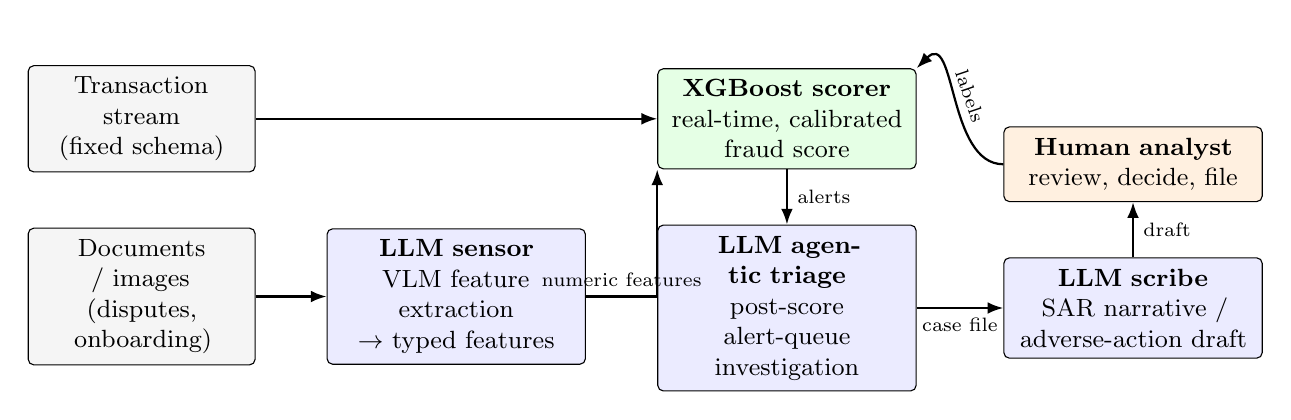
\begin{tikzpicture}[
  font=\small,
  node distance=7mm and 9mm,
  box/.style={draw, rounded corners=2pt, align=center, minimum height=9mm,
              inner sep=4pt, text width=30mm},
  llm/.style={box, fill=blue!8},
  tree/.style={box, fill=green!10},
  human/.style={box, fill=orange!12},
  data/.style={box, fill=gray!8, text width=26mm},
  arr/.style={-{Latex[length=2mm]}, thick}
]
\node[data] (txn) {Transaction stream\\(fixed schema)};
\node[data, below=of txn] (docs) {Documents / images\\(disputes, onboarding)};
\node[llm, right=of docs] (sensor) {\textbf{LLM sensor}\\VLM feature extraction\\$\to$ typed features};
\node[tree, right=of txn, xshift=42mm] (scorer) {\textbf{XGBoost scorer}\\real-time, calibrated\\fraud score};
\node[llm, below=of scorer] (triage) {\textbf{LLM agentic triage}\\post-score alert-queue\\investigation};
\node[llm, right=of triage, xshift=2mm] (scribe) {\textbf{LLM scribe}\\SAR narrative /\\adverse-action draft};
\node[human, above=of scribe] (analyst) {\textbf{Human analyst}\\review, decide, file};
\draw[arr] (txn) -- (scorer);
\draw[arr] (docs) -- (sensor);
\draw[arr] (sensor.east) -- node[above, sloped, font=\scriptsize]{numeric features} (scorer.west |- sensor.east) -- (scorer.south west);
\draw[arr] (scorer) -- node[right, font=\scriptsize]{alerts} (triage);
\draw[arr] (triage) -- node[below, font=\scriptsize]{case file} (scribe);
\draw[arr] (scribe) -- node[right, font=\scriptsize]{draft} (analyst);
\draw[arr] (analyst.west) to[out=180, in=45, looseness=1.1]
  node[above, sloped, font=\scriptsize]{labels} (scorer.north east);
\end{tikzpicture}}
\caption{The hybrid architecture. The LLM never sits in the synchronous scoring
path: the \emph{sensor} converts unstructured evidence to typed numeric
features upstream of the tree; the calibrated XGBoost \emph{scorer} owns the
real-time decision; the \emph{agentic triage} loop and the \emph{scribe}
operate post-score on the alert queue; the human analyst reviews drafts,
decides, files, and returns confirmed labels to retrain the scorer.}
\label{fig:p8-architecture}
\end{figure}

\paragraph{LLM as sensor.} Upstream of the tree, a vision--language model
consumes the unstructured evidence of \secref{sec:p8-gap-docs} and emits
\emph{typed features}: document-consistency scores, extracted field values,
tamper-likelihood indicators, mismatch flags. The interface is a fixed numeric
schema, so from the tree's perspective the VLM is just another feature source.
This placement has two consequences. First, the tree's accuracy and
calibration properties are preserved: the score is still produced by the model
family that wins the scorer seat. Second, the injection surface is contained:
adversarial text inside a document can at worst corrupt that document's
feature values---a bounded, per-case failure the tree averages over---rather
than hijack a decision-making agent, since the sensor has no tools, no memory
across cases, and no authority \citep{greshake2023injection}.

\paragraph{XGBoost as scorer.} The synchronous authorization path is unchanged
from the incumbent design: fixed-schema features (now augmented by sensor
outputs where evidence exists) enter a boosted tree; a calibrated score exits
in milliseconds at near-zero marginal cost. Nothing in the real-time loop
parses natural language. All four operational arguments of
\secref{sec:p8-scorer} are honored by construction.

\paragraph{Post-score agentic triage.} Alerts crossing the threshold enter a
queue where an LLM agent performs the mechanical investigation of
\secref{sec:p8-gap-agentic}: retrieving history, cross-referencing entities,
checking narrative consistency, and ranking the queue by investigative
priority with a written rationale per case. The agent is asynchronous
(seconds-to-minutes latency is acceptable), budget-capped (the token spend
lands only on the $\sim$1\% of traffic that alerts), and advisory (it cannot
close a case or file a report). Its cold-start mode (\secref{sec:p8-gap-coldstart})
runs the same loop seeded by typology bulletins instead of scorer alerts,
covering the label vacuum until confirmed cases retrain the tree.

\paragraph{LLM as scribe.} At the end of the queue, the scribe drafts the two
regulated documents of \secref{sec:p8-gap-narration}: the SAR narrative,
conditioned on the case file and structured to FinCEN's
who/what/when/where/why guidance \citep{fincen2003sarnarrative}; and, in
credit-decision contexts, the adverse-action statement of specific reasons,
conditioned on the tree's feature attributions so that the stated reasons are
the model's actual principal reasons as ECOA/Regulation~B demands
\citep{cfr1002_9, cfpb2022circular}. Every draft carries provenance links from
each claim to its evidence, and a human analyst signs before anything is
filed. The scribe is the highest-value, lowest-risk seat: pure text
generation, fully reviewable, in a category with no non-LLM competitor.

\paragraph{The label loop.} Analyst dispositions flow back as confirmed
labels, retraining the scorer and grading the sensor and triage components.
The architecture is thus not a static ensemble but a division of labor with a
single supervised spine: the tree learns from every closed case, and the LLM
seats are evaluated by how much they improve the tree's inputs, the queue's
ordering, and the filing's speed---each independently measurable, which is the
program discipline (``measure capability, don't trust the label'') applied to
the system's own components.
 \section{Compliance Grounding for the Scribe}
\label{sec:p8-compliance}

The scribe role rests on two bodies of U.S. regulation that oblige financial
institutions to produce specific prose. We cite the primary sources because
the paper's most durable claim---that narration is a task category no tree can
enter---is a legal fact before it is a modeling fact.

\subsection{SAR Narratives (Bank Secrecy Act / FinCEN)}
\label{sec:p8-sar}

Banks must report suspicious transactions to the Financial Crimes Enforcement
Network (FinCEN): under 31~C.F.R.~\S~1020.320, a bank must file a Suspicious
Activity Report for transactions of at least \$5{,}000 conducted at or through
the bank that it ``knows, suspects, or has reason to suspect'' involve illicit
funds, are designed to evade Bank Secrecy Act requirements, or have no
apparent lawful purpose, generally within 30 days of detection
\citep{cfr1020_320}. The report's decisive free-text component is the
narrative. FinCEN's guidance on preparing SAR narratives instructs filers to
identify the essential elements of the suspicious activity---who, what, when,
where, and why, along with the method of operation---in a complete,
self-contained account, and emphasizes that the narrative is where the filing
institution explains why the activity is suspicious
\citep{fincen2003sarnarrative}. This is precisely a conditional
text-generation task: given a case file, produce a complete, accurate,
element-covering narrative. Analyst backlogs make it a bottleneck; its
element-coverage structure makes it checkable; and emerging agentic systems
target exactly this drafting task \citep{naik2025coinvestigator}. Our
architecture keeps the human filer's judgment and signature---the LLM drafts,
the analyst verifies against the evidence links, and the institution files.

\subsection{Adverse-Action Notices (ECOA / Regulation B)}
\label{sec:p8-adverse}

When a creditor takes adverse action on a credit application, the Equal Credit
Opportunity Act as implemented by Regulation~B requires notification including
a statement of specific reasons (or disclosure of the right to obtain one):
under 12~C.F.R.~\S~1002.9, the statement of reasons ``must be specific and
indicate the principal reason(s) for the adverse action,'' and generic appeals
to internal standards or a failing score, without more, do not suffice
\citep{cfr1002_9}. The Consumer Financial Protection Bureau's Circular
2022-03 addresses the machine-learning case directly: the adverse-action
requirements apply regardless of the technology used, creditors may not rely
on ``black-box'' complexity as a defense, and a creditor that cannot state the
specific principal reasons behind its own model's decision is not excused but
non-compliant \citep{cfpb2022circular}.

Two design consequences follow for fraud-adjacent credit decisions. First, the
\emph{scorer} must remain a model whose principal reasons are extractable---a
gradient-boosted tree with feature attributions satisfies this far more
directly than an end-to-end LLM judgment whose verbalized rationale need not
correspond to its computation. Keeping XGBoost in the scorer seat is thus a
compliance posture, not only a performance one. Second, the \emph{scribe} must
be constrained to narrate the scorer's actual attributions: the LLM formats
and phrases the principal reasons; it must not invent them. The draft is
generated from the attribution vector, carries the attribution as provenance,
and is reviewed by a human before issuance. An LLM that freely composed
plausible-sounding reasons would be a Regulation~B violation generator; an LLM
that renders the tree's true top attributions into the required specific
statement is a compliance tool.

\paragraph{Scope note.} We cite U.S. federal requirements because they are the
sharpest published text-generation obligations in fraud and credit workflows;
analogous obligations exist in other jurisdictions but are not analyzed here.
Nothing in this section is legal advice; it establishes only that the
narration category exists, is mandatory, and is textual---hence enterable by
an LLM and not by a tree.
 \section{Related Work}
\label{sec:p8-related}

\paragraph{Gradient boosting on tabular data.} XGBoost
\citep{chen2016xgboost} remains the workhorse of applied tabular
classification. \citet{grinsztajn2022tree} show systematically that tree-based
models still outperform deep learning on medium-sized tabular benchmarks,
attributing the gap to trees' robustness to uninformative features and to the
non-smooth, non-rotation-invariant structure of tabular targets;
\citet{shwartzziv2021tabular} reach the same conclusion across deep tabular
architectures. Our scorer result is a single applied data point consistent
with this literature, with the added operational arguments (latency, cost,
calibration \citep{guo2017calibration}, injection surface
\citep{greshake2023injection}) that the benchmarking papers do not address.

\paragraph{LLMs for tabular data.} TabLLM \citep{hegselmann2023tabllm}
established the serialize-and-prompt recipe and showed it is most competitive
in very-few-shot regimes, degrading relative to boosted trees as labeled data
grows---exactly the pattern our head-to-head reproduces at $40{,}000$ labels,
and exactly why our taxonomy assigns the LLM the cold-start seat
(\secref{sec:p8-gap-coldstart}) rather than the scorer seat.

\paragraph{Fraud detection on transaction data.} \citet{dalpozzolo2018realistic}
give the canonical treatment of realistic credit-card fraud modeling---class
imbalance, verification latency, and concept drift---and motivate the
anonymized-feature, heavily imbalanced regime our synthetic benchmark
imitates. Our contribution is orthogonal to this line: we do not propose a
better detector but a division of labor around an already-strong one.

\paragraph{LLM agents for financial crime.} \citet{pirmorad2025icl_aml} shows
that LLMs prompted with serialized financial-graph neighborhoods can perform
analyst-style money-laundering triage few-shot, with coherent red-flag
justifications; \citet{naik2025coinvestigator} builds an agentic framework
specifically for drafting AML compliance narratives (SARs) with
human-in-the-loop review. These systems instantiate, respectively, our
cold-start and scribe/triage seats; our contribution is to place them in an
explicit architecture where the real-time scorer remains a tree.

\paragraph{VLMs for document and image fraud.} FakeShield
\citep{xu2024fakeshield} demonstrates explainable image-forgery detection and
localization with multimodal LLMs; Forensics-Bench \citep{wang2025forensicsbench}
benchmarks large vision--language models across 112 forgery types and finds
substantial headroom. Together they support both halves of our sensor claim:
VLMs uniquely extend the input space to raw document evidence, and their
current reliability justifies confining them to feature extraction with
downstream tree scoring and human review rather than autonomous verdicts.

\paragraph{Program context.} The parent reproducibility program measures
RL post-training claims capability-by-capability rather than by their labels;
the present side-probe applies the identical discipline to the marketing label
``AI'' in fraud detection. The methodological through-line is decomposition:
a bundled claim is replaced by per-capability measurements, and the deployment
decision is made seat by seat.
 \section{Limitations}
\label{sec:p8-limitations}

\paragraph{Custom synthetic dataset.} Our benchmark is generated by
\texttt{make\_classification} \citep{pedregosa2011sklearn}, not drawn from
production transactions. It reproduces the class imbalance and anonymized
feature shape of single-institution card-fraud data but none of its temporal
drift, verification latency, seasonality, or adversarial adaptation
\citep{dalpozzolo2018realistic}. The current artifact-backed AUCs
($0.7955$, $0.48268$) are therefore results on a stylized testbed and must not
be quoted as production expectations. The margin is dataset- and
environment-specific.

\paragraph{Historical numbers are records, not reproductions.} We could not
reconstruct the environment of the 21~June~2026 internal run that produced the
older $0.975$/$0.948$ pair, so those numbers are historical records, not
headline evidence. The paper's architectural conclusions are
insulated from this by design: the seat assignment rests on the latency, cost,
calibration, and injection arguments of \secref{sec:p8-scorer}, which apply at
accuracy parity and do not depend on the margin or its direction.

\paragraph{No cross-institution validation.} Everything here is one
configuration of one synthetic generator standing in for one institution's
feature view. Fraud patterns, feature pipelines, and base rates vary sharply
across issuers and geographies; the head-to-head has not been replicated on
any second data distribution, public benchmark, or real institution.

\paragraph{Cost estimates are internal.} The $\sim$$85\times$ agentic-triage
cost advantage (\secref{sec:p8-gap-agentic}) is an internal estimate built
from June-2026 token prices, assumed per-alert investigation times, and loaded
analyst compensation. Each assumption is contestable; none has been validated
in a production deployment; the figure is reported to one significant figure
and should be read as ``one to two orders of magnitude,'' not as a measured
constant. The latency and per-transaction cost contrasts of
\secref{sec:p8-scorer} are likewise operational characterizations, not
benchmarked service-level measurements.

\paragraph{Single LLM family, single recipe.} The $0.48268$ challenger is one
instruction-tuned LLM family under one serialization format and one
fine-tuning budget. We did not sweep model
families, scales, serializations, or prompting strategies, and stronger or
differently trained LLMs could narrow the accuracy gap. We note, however, that
the architecture's assignment of seats does not hinge on the gap: the
latency, cost, calibration, and injection arguments of \secref{sec:p8-scorer}
apply at accuracy parity.

\paragraph{Capability gaps argued, not all measured.} Of the four taxonomy
entries, only the scorer head-to-head carries a number of our own. The sensor,
scribe, and cold-start seats are grounded in external literature and primary
regulatory text rather than in our own end-to-end evaluations; the hybrid
architecture of \secref{sec:p8-architecture} is a design contribution whose
integrated performance is future work, not a deployed and audited system.
Nothing in \secref{sec:p8-compliance} is legal advice.
 \section{Conclusion and Future Work: Building the Hybrid}
\label{sec:p8-future}

The obvious next step is to build and measure the architecture rather than
argue it. Our plan, in the order the seats de-risk each other:

\begin{enumerate}[leftmargin=1.5em, itemsep=1pt, topsep=2pt]
\item \textbf{Sensor first.} Attach a VLM feature extractor to a
document-bearing subset of cases and measure the marginal AUC of
sensor-derived features \emph{inside the existing tree}---the cleanest test,
since the metric is the incumbent's own. This includes adversarial
evaluation: injected instructions inside documents must degrade at worst that
document's features \citep{greshake2023injection}.
\item \textbf{Scribe second.} Evaluate SAR-narrative drafts against FinCEN's
element-coverage structure (who/what/when/where/why/how)
\citep{fincen2003sarnarrative} with analyst-grader rubrics, and
adverse-action drafts for fidelity to the tree's actual attributions
\citep{cfr1002_9, cfpb2022circular}---measuring time-to-file and revision
distance, with a hard human sign-off gate.
\item \textbf{Triage third.} Replace the internal $85\times$ estimate with
measured per-alert token costs and analyst-minutes-saved on a live queue,
including the ordering quality of agent-ranked versus score-ranked queues.
\item \textbf{Cold-start last.} Simulate typology emergence by holding out a
generator cluster as an ``unseen scheme'' and measuring few-shot LLM detection
during the label vacuum, against the retrained tree's catch-up curve.
\end{enumerate}

Each experiment scores one seat with the seat's own metric---capability
measured, label ignored. If the program thesis holds anywhere outside RL
post-training, it should hold here: the pipeline that results is not ``AI
replacing the model'' but a tree that scores, an LLM that sees and writes, and
an analyst who decides. Until those experiments are run, the only artifact-backed
performance result is the synthetic-data scorer comparison; the sensor, scribe,
and triage seats remain design hypotheses rather than demonstrated deployment
gains.
 \bibliographystyle{plainnat}
\bibliography{references}
\end{document}
